\documentclass[twoside]{book}

% Packages required by doxygen
\usepackage{fixltx2e}
\usepackage{calc}
\usepackage{doxygen}
\usepackage[export]{adjustbox} % also loads graphicx
\usepackage{graphicx}
\usepackage[utf8]{inputenc}
\usepackage{makeidx}
\usepackage{multicol}
\usepackage{multirow}
\PassOptionsToPackage{warn}{textcomp}
\usepackage{textcomp}
\usepackage[nointegrals]{wasysym}
\usepackage[table]{xcolor}

% Font selection
\usepackage[T1]{fontenc}
\usepackage[scaled=.90]{helvet}
\usepackage{courier}
\usepackage{amssymb}
\usepackage{sectsty}
\renewcommand{\familydefault}{\sfdefault}
\allsectionsfont{%
  \fontseries{bc}\selectfont%
  \color{darkgray}%
}
\renewcommand{\DoxyLabelFont}{%
  \fontseries{bc}\selectfont%
  \color{darkgray}%
}
\newcommand{\+}{\discretionary{\mbox{\scriptsize$\hookleftarrow$}}{}{}}

% Page & text layout
\usepackage{geometry}
\geometry{%
  a4paper,%
  top=2.5cm,%
  bottom=2.5cm,%
  left=2.5cm,%
  right=2.5cm%
}
\tolerance=750
\hfuzz=15pt
\hbadness=750
\setlength{\emergencystretch}{15pt}
\setlength{\parindent}{0cm}
\setlength{\parskip}{0.2cm}
\makeatletter
\renewcommand{\paragraph}{%
  \@startsection{paragraph}{4}{0ex}{-1.0ex}{1.0ex}{%
    \normalfont\normalsize\bfseries\SS@parafont%
  }%
}
\renewcommand{\subparagraph}{%
  \@startsection{subparagraph}{5}{0ex}{-1.0ex}{1.0ex}{%
    \normalfont\normalsize\bfseries\SS@subparafont%
  }%
}
\makeatother

% Headers & footers
\usepackage{fancyhdr}
\pagestyle{fancyplain}
\fancyhead[LE]{\fancyplain{}{\bfseries\thepage}}
\fancyhead[CE]{\fancyplain{}{}}
\fancyhead[RE]{\fancyplain{}{\bfseries\leftmark}}
\fancyhead[LO]{\fancyplain{}{\bfseries\rightmark}}
\fancyhead[CO]{\fancyplain{}{}}
\fancyhead[RO]{\fancyplain{}{\bfseries\thepage}}
\fancyfoot[LE]{\fancyplain{}{}}
\fancyfoot[CE]{\fancyplain{}{}}
\fancyfoot[RE]{\fancyplain{}{\bfseries\scriptsize Generated on Fri Jan 2 2015 23\+:22\+:04 for My Project by Doxygen }}
\fancyfoot[LO]{\fancyplain{}{\bfseries\scriptsize Generated on Fri Jan 2 2015 23\+:22\+:04 for My Project by Doxygen }}
\fancyfoot[CO]{\fancyplain{}{}}
\fancyfoot[RO]{\fancyplain{}{}}
\renewcommand{\footrulewidth}{0.4pt}
\renewcommand{\chaptermark}[1]{%
  \markboth{#1}{}%
}
\renewcommand{\sectionmark}[1]{%
  \markright{\thesection\ #1}%
}

% Indices & bibliography
\usepackage{natbib}
\usepackage[titles]{tocloft}
\setcounter{tocdepth}{3}
\setcounter{secnumdepth}{5}
\makeindex

% Hyperlinks (required, but should be loaded last)
\usepackage{ifpdf}
\ifpdf
  \usepackage[pdftex,pagebackref=true]{hyperref}
\else
  \usepackage[ps2pdf,pagebackref=true]{hyperref}
\fi
\hypersetup{%
  colorlinks=true,%
  linkcolor=blue,%
  citecolor=blue,%
  unicode%
}

% Custom commands
\newcommand{\clearemptydoublepage}{%
  \newpage{\pagestyle{empty}\cleardoublepage}%
}


%===== C O N T E N T S =====

\begin{document}

% Titlepage & ToC
\hypersetup{pageanchor=false,
             bookmarks=true,
             bookmarksnumbered=true,
             pdfencoding=unicode
            }
\pagenumbering{roman}
\begin{titlepage}
\vspace*{7cm}
\begin{center}%
{\Large My Project }\\
\vspace*{1cm}
{\large Generated by Doxygen 1.8.9}\\
\vspace*{0.5cm}
{\small Fri Jan 2 2015 23:22:04}\\
\end{center}
\end{titlepage}
\clearemptydoublepage
\tableofcontents
\clearemptydoublepage
\pagenumbering{arabic}
\hypersetup{pageanchor=true}

%--- Begin generated contents ---
\chapter{Module Index}
\section{Modules}
Here is a list of all modules\+:\begin{DoxyCompactList}
\item \contentsline{section}{i8254}{\pageref{group__i8254}}{}
\item \contentsline{section}{lmlib}{\pageref{group__lmlib}}{}
\item \contentsline{section}{video\+\_\+gr}{\pageref{group__video__gr}}{}
\item \contentsline{section}{timer}{\pageref{group__timer}}{}
\item \contentsline{section}{vbe}{\pageref{group__vbe}}{}
\end{DoxyCompactList}

\chapter{Class Index}
\section{Class List}
Here are the classes, structs, unions and interfaces with brief descriptions\+:\begin{DoxyCompactList}
\item\contentsline{section}{\hyperlink{struct____attribute____}{\+\_\+\+\_\+attribute\+\_\+\+\_\+} }{\pageref{struct____attribute____}}{}
\item\contentsline{section}{\hyperlink{struct_buttons}{Buttons} }{\pageref{struct_buttons}}{}
\item\contentsline{section}{\hyperlink{struct_directories}{Directories} }{\pageref{struct_directories}}{}
\item\contentsline{section}{\hyperlink{structioboxes}{ioboxes} }{\pageref{structioboxes}}{}
\item\contentsline{section}{\hyperlink{structmmap__t}{mmap\+\_\+t} }{\pageref{structmmap__t}}{}
\item\contentsline{section}{\hyperlink{structmouse__state}{mouse\+\_\+state} }{\pageref{structmouse__state}}{}
\item\contentsline{section}{\hyperlink{structrtc__state}{rtc\+\_\+state} }{\pageref{structrtc__state}}{}
\item\contentsline{section}{\hyperlink{struct_sprite}{Sprite} }{\pageref{struct_sprite}}{}
\end{DoxyCompactList}

\chapter{File Index}
\section{File List}
Here is a list of all files with brief descriptions\+:\begin{DoxyCompactList}
\item\contentsline{section}{\hyperlink{headers_8h}{headers.\+h} }{\pageref{headers_8h}}{}
\item\contentsline{section}{\hyperlink{i8254_8h}{i8254.\+h} }{\pageref{i8254_8h}}{}
\item\contentsline{section}{\hyperlink{interface_8c}{interface.\+c} }{\pageref{interface_8c}}{}
\item\contentsline{section}{\hyperlink{interface_8h}{interface.\+h} }{\pageref{interface_8h}}{}
\item\contentsline{section}{\hyperlink{keyboard_8c}{keyboard.\+c} }{\pageref{keyboard_8c}}{}
\item\contentsline{section}{\hyperlink{keyboard_8h}{keyboard.\+h} }{\pageref{keyboard_8h}}{}
\item\contentsline{section}{\hyperlink{lmlib_8h}{lmlib.\+h} }{\pageref{lmlib_8h}}{}
\item\contentsline{section}{\hyperlink{logic_8c}{logic.\+c} }{\pageref{logic_8c}}{}
\item\contentsline{section}{\hyperlink{logic_8h}{logic.\+h} }{\pageref{logic_8h}}{}
\item\contentsline{section}{\hyperlink{main_8c}{main.\+c} }{\pageref{main_8c}}{}
\item\contentsline{section}{\hyperlink{mouse_8c}{mouse.\+c} }{\pageref{mouse_8c}}{}
\item\contentsline{section}{\hyperlink{mouse_8h}{mouse.\+h} }{\pageref{mouse_8h}}{}
\item\contentsline{section}{\hyperlink{pixmap_8c}{pixmap.\+c} }{\pageref{pixmap_8c}}{}
\item\contentsline{section}{\hyperlink{read__xpm_8c}{read\+\_\+xpm.\+c} }{\pageref{read__xpm_8c}}{}
\item\contentsline{section}{\hyperlink{read__xpm_8h}{read\+\_\+xpm.\+h} }{\pageref{read__xpm_8h}}{}
\item\contentsline{section}{\hyperlink{rtc_8c}{rtc.\+c} }{\pageref{rtc_8c}}{}
\item\contentsline{section}{\hyperlink{rtc_8h}{rtc.\+h} }{\pageref{rtc_8h}}{}
\item\contentsline{section}{\hyperlink{sprite_8c}{sprite.\+c} }{\pageref{sprite_8c}}{}
\item\contentsline{section}{\hyperlink{sprite_8h}{sprite.\+h} }{\pageref{sprite_8h}}{}
\item\contentsline{section}{\hyperlink{state_8c}{state.\+c} }{\pageref{state_8c}}{}
\item\contentsline{section}{\hyperlink{state_8h}{state.\+h} }{\pageref{state_8h}}{}
\item\contentsline{section}{\hyperlink{test5_8c}{test5.\+c} }{\pageref{test5_8c}}{}
\item\contentsline{section}{\hyperlink{test5_8h}{test5.\+h} }{\pageref{test5_8h}}{}
\item\contentsline{section}{\hyperlink{timer_8c}{timer.\+c} }{\pageref{timer_8c}}{}
\item\contentsline{section}{\hyperlink{timer_8h}{timer.\+h} }{\pageref{timer_8h}}{}
\item\contentsline{section}{\hyperlink{vbe_8c}{vbe.\+c} }{\pageref{vbe_8c}}{}
\item\contentsline{section}{\hyperlink{vbe_8h}{vbe.\+h} }{\pageref{vbe_8h}}{}
\item\contentsline{section}{\hyperlink{video__gr_8c}{video\+\_\+gr.\+c} }{\pageref{video__gr_8c}}{}
\item\contentsline{section}{\hyperlink{video__gr_8h}{video\+\_\+gr.\+h} }{\pageref{video__gr_8h}}{}
\end{DoxyCompactList}

\chapter{Module Documentation}
\hypertarget{group__i8254}{}\section{i8254}
\label{group__i8254}\index{i8254@{i8254}}
\subsection*{Macros}
\begin{DoxyCompactItemize}
\item 
\#define \hyperlink{group__i8254_ga8d842ab28d8f573d16da7b28b36e2460}{C\+H\+E\+C\+K\+\_\+\+B\+I\+T}(var,  pos)~((var) \& (1$<$$<$(pos)))
\item 
\#define \hyperlink{group__i8254_gacf926951944b6cf370b7229ebd50dd8b}{T\+I\+M\+E\+R\+\_\+\+F\+R\+E\+Q}~1193182
\begin{DoxyCompactList}\small\item\em clock frequency for timer in P\+C and A\+T \end{DoxyCompactList}\item 
\#define \hyperlink{group__i8254_ga3a8ea58898cb58fc96013383d39f482c}{B\+I\+T}(n)~(0x01$<$$<$(n))
\item 
\#define \hyperlink{group__i8254_ga30bf84c312af248cb81bb224e09f9ba8}{T\+I\+M\+E\+R0\+\_\+\+I\+R\+Q}~0
\begin{DoxyCompactList}\small\item\em Timer 0 I\+R\+Q line. \end{DoxyCompactList}\item 
\#define \hyperlink{group__i8254_gacc9ff9df4a9674a1ce9ba08fc4a4679e}{T\+I\+M\+E\+R\+\_\+0}~0x40
\begin{DoxyCompactList}\small\item\em Timer 0 count register. \end{DoxyCompactList}\item 
\#define \hyperlink{group__i8254_gac62c99c2a9289891c1b83052242cca49}{T\+I\+M\+E\+R\+\_\+1}~0x41
\begin{DoxyCompactList}\small\item\em Timer 1 count register. \end{DoxyCompactList}\item 
\#define \hyperlink{group__i8254_ga1f34f18ad0ab8cace46b615773b48735}{T\+I\+M\+E\+R\+\_\+2}~0x42
\begin{DoxyCompactList}\small\item\em Timer 2 count register. \end{DoxyCompactList}\item 
\#define \hyperlink{group__i8254_ga282832448fb0281ef53d243c1cd48491}{T\+I\+M\+E\+R\+\_\+\+C\+T\+R\+L}~0x43
\begin{DoxyCompactList}\small\item\em Control register. \end{DoxyCompactList}\item 
\#define \hyperlink{group__i8254_ga51b3a5e3d4811ca063fe25e35560ab40}{S\+P\+E\+A\+K\+E\+R\+\_\+\+C\+T\+R\+L}~0x61
\begin{DoxyCompactList}\small\item\em Register for speaker control. \end{DoxyCompactList}\item 
\#define \hyperlink{group__i8254_ga6a4822642d40c248435692324a818010}{T\+I\+M\+E\+R\+\_\+\+S\+E\+L0}~0x00
\begin{DoxyCompactList}\small\item\em Control Word for Timer 0. \end{DoxyCompactList}\item 
\#define \hyperlink{group__i8254_ga8349623fd8d99f9cc5d8ae29d78594fc}{T\+I\+M\+E\+R\+\_\+\+S\+E\+L1}~\hyperlink{group__i8254_ga3a8ea58898cb58fc96013383d39f482c}{B\+I\+T}(6)
\begin{DoxyCompactList}\small\item\em Control Word for Timer 1. \end{DoxyCompactList}\item 
\#define \hyperlink{group__i8254_ga142a255de0dbc48aeabd45fc10c33672}{T\+I\+M\+E\+R\+\_\+\+S\+E\+L2}~\hyperlink{group__i8254_ga3a8ea58898cb58fc96013383d39f482c}{B\+I\+T}(7)
\begin{DoxyCompactList}\small\item\em Control Word for Timer 2. \end{DoxyCompactList}\item 
\#define \hyperlink{group__i8254_ga4c2eecbfb96744a9c2af71dba75ecb18}{T\+I\+M\+E\+R\+\_\+\+R\+B\+\_\+\+C\+M\+D}~(\hyperlink{group__i8254_ga3a8ea58898cb58fc96013383d39f482c}{B\+I\+T}(7)$\vert$\hyperlink{group__i8254_ga3a8ea58898cb58fc96013383d39f482c}{B\+I\+T}(6))
\begin{DoxyCompactList}\small\item\em Read Back Command. \end{DoxyCompactList}\item 
\#define \hyperlink{group__i8254_gac18cb814ebd0d67235392c330e0e3504}{T\+I\+M\+E\+R\+\_\+\+L\+S\+B}~\hyperlink{group__i8254_ga3a8ea58898cb58fc96013383d39f482c}{B\+I\+T}(4)
\begin{DoxyCompactList}\small\item\em Initialize Counter L\+S\+B only. \end{DoxyCompactList}\item 
\#define \hyperlink{group__i8254_ga2a8a6d363c612d756cd8d78480f7cd04}{T\+I\+M\+E\+R\+\_\+\+M\+S\+B}~\hyperlink{group__i8254_ga3a8ea58898cb58fc96013383d39f482c}{B\+I\+T}(5)
\begin{DoxyCompactList}\small\item\em Initialize Counter M\+S\+B only. \end{DoxyCompactList}\item 
\#define \hyperlink{group__i8254_ga8c0f1933323274c765e23837e4fbc8c7}{T\+I\+M\+E\+R\+\_\+\+L\+S\+B\+\_\+\+M\+S\+B}~(\hyperlink{group__i8254_gac18cb814ebd0d67235392c330e0e3504}{T\+I\+M\+E\+R\+\_\+\+L\+S\+B} $\vert$ \hyperlink{group__i8254_ga2a8a6d363c612d756cd8d78480f7cd04}{T\+I\+M\+E\+R\+\_\+\+M\+S\+B})
\begin{DoxyCompactList}\small\item\em Initialize L\+S\+B first and M\+S\+B afterwards. \end{DoxyCompactList}\item 
\#define \hyperlink{group__i8254_ga4745cbf21da3d3fea5dbb080b2b73bac}{T\+I\+M\+E\+R\+\_\+\+S\+Q\+R\+\_\+\+W\+A\+V\+E}~(\hyperlink{group__i8254_ga3a8ea58898cb58fc96013383d39f482c}{B\+I\+T}(2)$\vert$\hyperlink{group__i8254_ga3a8ea58898cb58fc96013383d39f482c}{B\+I\+T}(1))
\begin{DoxyCompactList}\small\item\em Mode 3\+: square wave generator. \end{DoxyCompactList}\item 
\#define \hyperlink{group__i8254_ga5d4449e0fa1cf4a4d107a48a04a1265f}{T\+I\+M\+E\+R\+\_\+\+R\+A\+T\+E\+\_\+\+G\+E\+N}~\hyperlink{group__i8254_ga3a8ea58898cb58fc96013383d39f482c}{B\+I\+T}(2)
\begin{DoxyCompactList}\small\item\em Mode 2\+: rate generator. \end{DoxyCompactList}\item 
\#define \hyperlink{group__i8254_ga325b992a371d5d981c4eceff42fa5956}{T\+I\+M\+E\+R\+\_\+\+B\+C\+D}~0x01
\begin{DoxyCompactList}\small\item\em Count in B\+C\+D. \end{DoxyCompactList}\item 
\#define \hyperlink{group__i8254_gad2913dcf2f91453317bd035589ac0a7d}{T\+I\+M\+E\+R\+\_\+\+B\+I\+N}~0x00
\begin{DoxyCompactList}\small\item\em Count in binary. \end{DoxyCompactList}\item 
\#define \hyperlink{group__i8254_ga6c248216df24b5e9d907d126d80bd195}{T\+I\+M\+E\+R\+\_\+\+R\+B\+\_\+\+C\+O\+U\+N\+T\+\_\+}~\hyperlink{group__i8254_ga3a8ea58898cb58fc96013383d39f482c}{B\+I\+T}(5)
\item 
\#define \hyperlink{group__i8254_ga08b4952bb7058684a3f8f66be04dd45e}{T\+I\+M\+E\+R\+\_\+\+R\+B\+\_\+\+S\+T\+A\+T\+U\+S\+\_\+}~\hyperlink{group__i8254_ga3a8ea58898cb58fc96013383d39f482c}{B\+I\+T}(4)
\item 
\#define \hyperlink{group__i8254_gaf598b17740e07842a0545af512714711}{T\+I\+M\+E\+R\+\_\+\+R\+B\+\_\+\+S\+E\+L}(n)~\hyperlink{group__i8254_ga3a8ea58898cb58fc96013383d39f482c}{B\+I\+T}((n)+1)
\end{DoxyCompactItemize}


\subsection{Detailed Description}
Constants for programming the i8254 Timer. Needs to be completed. 

\subsection{Macro Definition Documentation}
\hypertarget{group__i8254_ga3a8ea58898cb58fc96013383d39f482c}{}\index{i8254@{i8254}!B\+I\+T@{B\+I\+T}}
\index{B\+I\+T@{B\+I\+T}!i8254@{i8254}}
\subsubsection[{B\+I\+T}]{\setlength{\rightskip}{0pt plus 5cm}\#define B\+I\+T(
\begin{DoxyParamCaption}
\item[{}]{n}
\end{DoxyParamCaption}
)~(0x01$<$$<$(n))}\label{group__i8254_ga3a8ea58898cb58fc96013383d39f482c}


Definition at line 19 of file i8254.\+h.

\hypertarget{group__i8254_ga8d842ab28d8f573d16da7b28b36e2460}{}\index{i8254@{i8254}!C\+H\+E\+C\+K\+\_\+\+B\+I\+T@{C\+H\+E\+C\+K\+\_\+\+B\+I\+T}}
\index{C\+H\+E\+C\+K\+\_\+\+B\+I\+T@{C\+H\+E\+C\+K\+\_\+\+B\+I\+T}!i8254@{i8254}}
\subsubsection[{C\+H\+E\+C\+K\+\_\+\+B\+I\+T}]{\setlength{\rightskip}{0pt plus 5cm}\#define C\+H\+E\+C\+K\+\_\+\+B\+I\+T(
\begin{DoxyParamCaption}
\item[{}]{var, }
\item[{}]{pos}
\end{DoxyParamCaption}
)~((var) \& (1$<$$<$(pos)))}\label{group__i8254_ga8d842ab28d8f573d16da7b28b36e2460}


Definition at line 13 of file i8254.\+h.

\hypertarget{group__i8254_ga51b3a5e3d4811ca063fe25e35560ab40}{}\index{i8254@{i8254}!S\+P\+E\+A\+K\+E\+R\+\_\+\+C\+T\+R\+L@{S\+P\+E\+A\+K\+E\+R\+\_\+\+C\+T\+R\+L}}
\index{S\+P\+E\+A\+K\+E\+R\+\_\+\+C\+T\+R\+L@{S\+P\+E\+A\+K\+E\+R\+\_\+\+C\+T\+R\+L}!i8254@{i8254}}
\subsubsection[{S\+P\+E\+A\+K\+E\+R\+\_\+\+C\+T\+R\+L}]{\setlength{\rightskip}{0pt plus 5cm}\#define S\+P\+E\+A\+K\+E\+R\+\_\+\+C\+T\+R\+L~0x61}\label{group__i8254_ga51b3a5e3d4811ca063fe25e35560ab40}


Register for speaker control. 



Definition at line 30 of file i8254.\+h.

\hypertarget{group__i8254_ga30bf84c312af248cb81bb224e09f9ba8}{}\index{i8254@{i8254}!T\+I\+M\+E\+R0\+\_\+\+I\+R\+Q@{T\+I\+M\+E\+R0\+\_\+\+I\+R\+Q}}
\index{T\+I\+M\+E\+R0\+\_\+\+I\+R\+Q@{T\+I\+M\+E\+R0\+\_\+\+I\+R\+Q}!i8254@{i8254}}
\subsubsection[{T\+I\+M\+E\+R0\+\_\+\+I\+R\+Q}]{\setlength{\rightskip}{0pt plus 5cm}\#define T\+I\+M\+E\+R0\+\_\+\+I\+R\+Q~0}\label{group__i8254_ga30bf84c312af248cb81bb224e09f9ba8}


Timer 0 I\+R\+Q line. 



Definition at line 21 of file i8254.\+h.

\hypertarget{group__i8254_gacc9ff9df4a9674a1ce9ba08fc4a4679e}{}\index{i8254@{i8254}!T\+I\+M\+E\+R\+\_\+0@{T\+I\+M\+E\+R\+\_\+0}}
\index{T\+I\+M\+E\+R\+\_\+0@{T\+I\+M\+E\+R\+\_\+0}!i8254@{i8254}}
\subsubsection[{T\+I\+M\+E\+R\+\_\+0}]{\setlength{\rightskip}{0pt plus 5cm}\#define T\+I\+M\+E\+R\+\_\+0~0x40}\label{group__i8254_gacc9ff9df4a9674a1ce9ba08fc4a4679e}


Timer 0 count register. 



Definition at line 25 of file i8254.\+h.

\hypertarget{group__i8254_gac62c99c2a9289891c1b83052242cca49}{}\index{i8254@{i8254}!T\+I\+M\+E\+R\+\_\+1@{T\+I\+M\+E\+R\+\_\+1}}
\index{T\+I\+M\+E\+R\+\_\+1@{T\+I\+M\+E\+R\+\_\+1}!i8254@{i8254}}
\subsubsection[{T\+I\+M\+E\+R\+\_\+1}]{\setlength{\rightskip}{0pt plus 5cm}\#define T\+I\+M\+E\+R\+\_\+1~0x41}\label{group__i8254_gac62c99c2a9289891c1b83052242cca49}


Timer 1 count register. 



Definition at line 26 of file i8254.\+h.

\hypertarget{group__i8254_ga1f34f18ad0ab8cace46b615773b48735}{}\index{i8254@{i8254}!T\+I\+M\+E\+R\+\_\+2@{T\+I\+M\+E\+R\+\_\+2}}
\index{T\+I\+M\+E\+R\+\_\+2@{T\+I\+M\+E\+R\+\_\+2}!i8254@{i8254}}
\subsubsection[{T\+I\+M\+E\+R\+\_\+2}]{\setlength{\rightskip}{0pt plus 5cm}\#define T\+I\+M\+E\+R\+\_\+2~0x42}\label{group__i8254_ga1f34f18ad0ab8cace46b615773b48735}


Timer 2 count register. 



Definition at line 27 of file i8254.\+h.

\hypertarget{group__i8254_ga325b992a371d5d981c4eceff42fa5956}{}\index{i8254@{i8254}!T\+I\+M\+E\+R\+\_\+\+B\+C\+D@{T\+I\+M\+E\+R\+\_\+\+B\+C\+D}}
\index{T\+I\+M\+E\+R\+\_\+\+B\+C\+D@{T\+I\+M\+E\+R\+\_\+\+B\+C\+D}!i8254@{i8254}}
\subsubsection[{T\+I\+M\+E\+R\+\_\+\+B\+C\+D}]{\setlength{\rightskip}{0pt plus 5cm}\#define T\+I\+M\+E\+R\+\_\+\+B\+C\+D~0x01}\label{group__i8254_ga325b992a371d5d981c4eceff42fa5956}


Count in B\+C\+D. 



Definition at line 54 of file i8254.\+h.

\hypertarget{group__i8254_gad2913dcf2f91453317bd035589ac0a7d}{}\index{i8254@{i8254}!T\+I\+M\+E\+R\+\_\+\+B\+I\+N@{T\+I\+M\+E\+R\+\_\+\+B\+I\+N}}
\index{T\+I\+M\+E\+R\+\_\+\+B\+I\+N@{T\+I\+M\+E\+R\+\_\+\+B\+I\+N}!i8254@{i8254}}
\subsubsection[{T\+I\+M\+E\+R\+\_\+\+B\+I\+N}]{\setlength{\rightskip}{0pt plus 5cm}\#define T\+I\+M\+E\+R\+\_\+\+B\+I\+N~0x00}\label{group__i8254_gad2913dcf2f91453317bd035589ac0a7d}


Count in binary. 



Definition at line 55 of file i8254.\+h.

\hypertarget{group__i8254_ga282832448fb0281ef53d243c1cd48491}{}\index{i8254@{i8254}!T\+I\+M\+E\+R\+\_\+\+C\+T\+R\+L@{T\+I\+M\+E\+R\+\_\+\+C\+T\+R\+L}}
\index{T\+I\+M\+E\+R\+\_\+\+C\+T\+R\+L@{T\+I\+M\+E\+R\+\_\+\+C\+T\+R\+L}!i8254@{i8254}}
\subsubsection[{T\+I\+M\+E\+R\+\_\+\+C\+T\+R\+L}]{\setlength{\rightskip}{0pt plus 5cm}\#define T\+I\+M\+E\+R\+\_\+\+C\+T\+R\+L~0x43}\label{group__i8254_ga282832448fb0281ef53d243c1cd48491}


Control register. 



Definition at line 28 of file i8254.\+h.

\hypertarget{group__i8254_gacf926951944b6cf370b7229ebd50dd8b}{}\index{i8254@{i8254}!T\+I\+M\+E\+R\+\_\+\+F\+R\+E\+Q@{T\+I\+M\+E\+R\+\_\+\+F\+R\+E\+Q}}
\index{T\+I\+M\+E\+R\+\_\+\+F\+R\+E\+Q@{T\+I\+M\+E\+R\+\_\+\+F\+R\+E\+Q}!i8254@{i8254}}
\subsubsection[{T\+I\+M\+E\+R\+\_\+\+F\+R\+E\+Q}]{\setlength{\rightskip}{0pt plus 5cm}\#define T\+I\+M\+E\+R\+\_\+\+F\+R\+E\+Q~1193182}\label{group__i8254_gacf926951944b6cf370b7229ebd50dd8b}


clock frequency for timer in P\+C and A\+T 



Definition at line 17 of file i8254.\+h.

\hypertarget{group__i8254_gac18cb814ebd0d67235392c330e0e3504}{}\index{i8254@{i8254}!T\+I\+M\+E\+R\+\_\+\+L\+S\+B@{T\+I\+M\+E\+R\+\_\+\+L\+S\+B}}
\index{T\+I\+M\+E\+R\+\_\+\+L\+S\+B@{T\+I\+M\+E\+R\+\_\+\+L\+S\+B}!i8254@{i8254}}
\subsubsection[{T\+I\+M\+E\+R\+\_\+\+L\+S\+B}]{\setlength{\rightskip}{0pt plus 5cm}\#define T\+I\+M\+E\+R\+\_\+\+L\+S\+B~{\bf B\+I\+T}(4)}\label{group__i8254_gac18cb814ebd0d67235392c330e0e3504}


Initialize Counter L\+S\+B only. 



Definition at line 43 of file i8254.\+h.

\hypertarget{group__i8254_ga8c0f1933323274c765e23837e4fbc8c7}{}\index{i8254@{i8254}!T\+I\+M\+E\+R\+\_\+\+L\+S\+B\+\_\+\+M\+S\+B@{T\+I\+M\+E\+R\+\_\+\+L\+S\+B\+\_\+\+M\+S\+B}}
\index{T\+I\+M\+E\+R\+\_\+\+L\+S\+B\+\_\+\+M\+S\+B@{T\+I\+M\+E\+R\+\_\+\+L\+S\+B\+\_\+\+M\+S\+B}!i8254@{i8254}}
\subsubsection[{T\+I\+M\+E\+R\+\_\+\+L\+S\+B\+\_\+\+M\+S\+B}]{\setlength{\rightskip}{0pt plus 5cm}\#define T\+I\+M\+E\+R\+\_\+\+L\+S\+B\+\_\+\+M\+S\+B~({\bf T\+I\+M\+E\+R\+\_\+\+L\+S\+B} $\vert$ {\bf T\+I\+M\+E\+R\+\_\+\+M\+S\+B})}\label{group__i8254_ga8c0f1933323274c765e23837e4fbc8c7}


Initialize L\+S\+B first and M\+S\+B afterwards. 



Definition at line 45 of file i8254.\+h.

\hypertarget{group__i8254_ga2a8a6d363c612d756cd8d78480f7cd04}{}\index{i8254@{i8254}!T\+I\+M\+E\+R\+\_\+\+M\+S\+B@{T\+I\+M\+E\+R\+\_\+\+M\+S\+B}}
\index{T\+I\+M\+E\+R\+\_\+\+M\+S\+B@{T\+I\+M\+E\+R\+\_\+\+M\+S\+B}!i8254@{i8254}}
\subsubsection[{T\+I\+M\+E\+R\+\_\+\+M\+S\+B}]{\setlength{\rightskip}{0pt plus 5cm}\#define T\+I\+M\+E\+R\+\_\+\+M\+S\+B~{\bf B\+I\+T}(5)}\label{group__i8254_ga2a8a6d363c612d756cd8d78480f7cd04}


Initialize Counter M\+S\+B only. 



Definition at line 44 of file i8254.\+h.

\hypertarget{group__i8254_ga5d4449e0fa1cf4a4d107a48a04a1265f}{}\index{i8254@{i8254}!T\+I\+M\+E\+R\+\_\+\+R\+A\+T\+E\+\_\+\+G\+E\+N@{T\+I\+M\+E\+R\+\_\+\+R\+A\+T\+E\+\_\+\+G\+E\+N}}
\index{T\+I\+M\+E\+R\+\_\+\+R\+A\+T\+E\+\_\+\+G\+E\+N@{T\+I\+M\+E\+R\+\_\+\+R\+A\+T\+E\+\_\+\+G\+E\+N}!i8254@{i8254}}
\subsubsection[{T\+I\+M\+E\+R\+\_\+\+R\+A\+T\+E\+\_\+\+G\+E\+N}]{\setlength{\rightskip}{0pt plus 5cm}\#define T\+I\+M\+E\+R\+\_\+\+R\+A\+T\+E\+\_\+\+G\+E\+N~{\bf B\+I\+T}(2)}\label{group__i8254_ga5d4449e0fa1cf4a4d107a48a04a1265f}


Mode 2\+: rate generator. 



Definition at line 50 of file i8254.\+h.

\hypertarget{group__i8254_ga4c2eecbfb96744a9c2af71dba75ecb18}{}\index{i8254@{i8254}!T\+I\+M\+E\+R\+\_\+\+R\+B\+\_\+\+C\+M\+D@{T\+I\+M\+E\+R\+\_\+\+R\+B\+\_\+\+C\+M\+D}}
\index{T\+I\+M\+E\+R\+\_\+\+R\+B\+\_\+\+C\+M\+D@{T\+I\+M\+E\+R\+\_\+\+R\+B\+\_\+\+C\+M\+D}!i8254@{i8254}}
\subsubsection[{T\+I\+M\+E\+R\+\_\+\+R\+B\+\_\+\+C\+M\+D}]{\setlength{\rightskip}{0pt plus 5cm}\#define T\+I\+M\+E\+R\+\_\+\+R\+B\+\_\+\+C\+M\+D~({\bf B\+I\+T}(7)$\vert${\bf B\+I\+T}(6))}\label{group__i8254_ga4c2eecbfb96744a9c2af71dba75ecb18}


Read Back Command. 



Definition at line 39 of file i8254.\+h.

\hypertarget{group__i8254_ga6c248216df24b5e9d907d126d80bd195}{}\index{i8254@{i8254}!T\+I\+M\+E\+R\+\_\+\+R\+B\+\_\+\+C\+O\+U\+N\+T\+\_\+@{T\+I\+M\+E\+R\+\_\+\+R\+B\+\_\+\+C\+O\+U\+N\+T\+\_\+}}
\index{T\+I\+M\+E\+R\+\_\+\+R\+B\+\_\+\+C\+O\+U\+N\+T\+\_\+@{T\+I\+M\+E\+R\+\_\+\+R\+B\+\_\+\+C\+O\+U\+N\+T\+\_\+}!i8254@{i8254}}
\subsubsection[{T\+I\+M\+E\+R\+\_\+\+R\+B\+\_\+\+C\+O\+U\+N\+T\+\_\+}]{\setlength{\rightskip}{0pt plus 5cm}\#define T\+I\+M\+E\+R\+\_\+\+R\+B\+\_\+\+C\+O\+U\+N\+T\+\_\+~{\bf B\+I\+T}(5)}\label{group__i8254_ga6c248216df24b5e9d907d126d80bd195}


Definition at line 59 of file i8254.\+h.

\hypertarget{group__i8254_gaf598b17740e07842a0545af512714711}{}\index{i8254@{i8254}!T\+I\+M\+E\+R\+\_\+\+R\+B\+\_\+\+S\+E\+L@{T\+I\+M\+E\+R\+\_\+\+R\+B\+\_\+\+S\+E\+L}}
\index{T\+I\+M\+E\+R\+\_\+\+R\+B\+\_\+\+S\+E\+L@{T\+I\+M\+E\+R\+\_\+\+R\+B\+\_\+\+S\+E\+L}!i8254@{i8254}}
\subsubsection[{T\+I\+M\+E\+R\+\_\+\+R\+B\+\_\+\+S\+E\+L}]{\setlength{\rightskip}{0pt plus 5cm}\#define T\+I\+M\+E\+R\+\_\+\+R\+B\+\_\+\+S\+E\+L(
\begin{DoxyParamCaption}
\item[{}]{n}
\end{DoxyParamCaption}
)~{\bf B\+I\+T}((n)+1)}\label{group__i8254_gaf598b17740e07842a0545af512714711}


Definition at line 61 of file i8254.\+h.

\hypertarget{group__i8254_ga08b4952bb7058684a3f8f66be04dd45e}{}\index{i8254@{i8254}!T\+I\+M\+E\+R\+\_\+\+R\+B\+\_\+\+S\+T\+A\+T\+U\+S\+\_\+@{T\+I\+M\+E\+R\+\_\+\+R\+B\+\_\+\+S\+T\+A\+T\+U\+S\+\_\+}}
\index{T\+I\+M\+E\+R\+\_\+\+R\+B\+\_\+\+S\+T\+A\+T\+U\+S\+\_\+@{T\+I\+M\+E\+R\+\_\+\+R\+B\+\_\+\+S\+T\+A\+T\+U\+S\+\_\+}!i8254@{i8254}}
\subsubsection[{T\+I\+M\+E\+R\+\_\+\+R\+B\+\_\+\+S\+T\+A\+T\+U\+S\+\_\+}]{\setlength{\rightskip}{0pt plus 5cm}\#define T\+I\+M\+E\+R\+\_\+\+R\+B\+\_\+\+S\+T\+A\+T\+U\+S\+\_\+~{\bf B\+I\+T}(4)}\label{group__i8254_ga08b4952bb7058684a3f8f66be04dd45e}


Definition at line 60 of file i8254.\+h.

\hypertarget{group__i8254_ga6a4822642d40c248435692324a818010}{}\index{i8254@{i8254}!T\+I\+M\+E\+R\+\_\+\+S\+E\+L0@{T\+I\+M\+E\+R\+\_\+\+S\+E\+L0}}
\index{T\+I\+M\+E\+R\+\_\+\+S\+E\+L0@{T\+I\+M\+E\+R\+\_\+\+S\+E\+L0}!i8254@{i8254}}
\subsubsection[{T\+I\+M\+E\+R\+\_\+\+S\+E\+L0}]{\setlength{\rightskip}{0pt plus 5cm}\#define T\+I\+M\+E\+R\+\_\+\+S\+E\+L0~0x00}\label{group__i8254_ga6a4822642d40c248435692324a818010}


Control Word for Timer 0. 



Definition at line 36 of file i8254.\+h.

\hypertarget{group__i8254_ga8349623fd8d99f9cc5d8ae29d78594fc}{}\index{i8254@{i8254}!T\+I\+M\+E\+R\+\_\+\+S\+E\+L1@{T\+I\+M\+E\+R\+\_\+\+S\+E\+L1}}
\index{T\+I\+M\+E\+R\+\_\+\+S\+E\+L1@{T\+I\+M\+E\+R\+\_\+\+S\+E\+L1}!i8254@{i8254}}
\subsubsection[{T\+I\+M\+E\+R\+\_\+\+S\+E\+L1}]{\setlength{\rightskip}{0pt plus 5cm}\#define T\+I\+M\+E\+R\+\_\+\+S\+E\+L1~{\bf B\+I\+T}(6)}\label{group__i8254_ga8349623fd8d99f9cc5d8ae29d78594fc}


Control Word for Timer 1. 



Definition at line 37 of file i8254.\+h.

\hypertarget{group__i8254_ga142a255de0dbc48aeabd45fc10c33672}{}\index{i8254@{i8254}!T\+I\+M\+E\+R\+\_\+\+S\+E\+L2@{T\+I\+M\+E\+R\+\_\+\+S\+E\+L2}}
\index{T\+I\+M\+E\+R\+\_\+\+S\+E\+L2@{T\+I\+M\+E\+R\+\_\+\+S\+E\+L2}!i8254@{i8254}}
\subsubsection[{T\+I\+M\+E\+R\+\_\+\+S\+E\+L2}]{\setlength{\rightskip}{0pt plus 5cm}\#define T\+I\+M\+E\+R\+\_\+\+S\+E\+L2~{\bf B\+I\+T}(7)}\label{group__i8254_ga142a255de0dbc48aeabd45fc10c33672}


Control Word for Timer 2. 



Definition at line 38 of file i8254.\+h.

\hypertarget{group__i8254_ga4745cbf21da3d3fea5dbb080b2b73bac}{}\index{i8254@{i8254}!T\+I\+M\+E\+R\+\_\+\+S\+Q\+R\+\_\+\+W\+A\+V\+E@{T\+I\+M\+E\+R\+\_\+\+S\+Q\+R\+\_\+\+W\+A\+V\+E}}
\index{T\+I\+M\+E\+R\+\_\+\+S\+Q\+R\+\_\+\+W\+A\+V\+E@{T\+I\+M\+E\+R\+\_\+\+S\+Q\+R\+\_\+\+W\+A\+V\+E}!i8254@{i8254}}
\subsubsection[{T\+I\+M\+E\+R\+\_\+\+S\+Q\+R\+\_\+\+W\+A\+V\+E}]{\setlength{\rightskip}{0pt plus 5cm}\#define T\+I\+M\+E\+R\+\_\+\+S\+Q\+R\+\_\+\+W\+A\+V\+E~({\bf B\+I\+T}(2)$\vert${\bf B\+I\+T}(1))}\label{group__i8254_ga4745cbf21da3d3fea5dbb080b2b73bac}


Mode 3\+: square wave generator. 



Definition at line 49 of file i8254.\+h.


\hypertarget{group__lmlib}{}\section{lmlib}
\label{group__lmlib}\index{lmlib@{lmlib}}
\subsection*{Classes}
\begin{DoxyCompactItemize}
\item 
struct \hyperlink{structmmap__t}{mmap\+\_\+t}
\end{DoxyCompactItemize}
\subsection*{Functions}
\begin{DoxyCompactItemize}
\item 
void $\ast$ \hyperlink{group__lmlib_ga00a9c17c01e794a6bfc80fc5c6ab1ed1}{lm\+\_\+init} (void)
\begin{DoxyCompactList}\small\item\em Initializes the low memory area, the region up to the 1 M\+Byte physical address, by mapping it on the process\textquotesingle{} physical memory address. \end{DoxyCompactList}\item 
void $\ast$ \hyperlink{group__lmlib_gae45d971ce2ffcf4dc2677eba033a92cd}{lm\+\_\+alloc} (unsigned long size, \hyperlink{structmmap__t}{mmap\+\_\+t} $\ast$map)
\begin{DoxyCompactList}\small\item\em Allocates a memory block in low memory area with the specified size. \end{DoxyCompactList}\item 
void \hyperlink{group__lmlib_ga73e89d9c297b7390021fb545513579c6}{lm\+\_\+free} (\hyperlink{structmmap__t}{mmap\+\_\+t} $\ast$map)
\begin{DoxyCompactList}\small\item\em Frees a memory block in the low memory area, previously allocated using \hyperlink{group__lmlib_gae45d971ce2ffcf4dc2677eba033a92cd}{lm\+\_\+alloc()} \end{DoxyCompactList}\end{DoxyCompactItemize}
\subsection*{Variables}
\begin{DoxyCompactItemize}
\item 
phys\+\_\+bytes \hyperlink{group__lmlib_gaa6ac1ee0e0fadea4a4f85b48c8359ae4}{mmap\+\_\+t\+::phys}
\begin{DoxyCompactList}\small\item\em physical address \end{DoxyCompactList}\item 
void $\ast$ \hyperlink{group__lmlib_ga4de93144fb3ffbceb9bd1f3009d6d98c}{mmap\+\_\+t\+::virtual}
\begin{DoxyCompactList}\small\item\em virtual address \end{DoxyCompactList}\item 
unsigned long \hyperlink{group__lmlib_gaf1cdc5384a402fddf33f400a5e1e5e45}{mmap\+\_\+t\+::size}
\begin{DoxyCompactList}\small\item\em size of memory region \end{DoxyCompactList}\end{DoxyCompactItemize}


\subsection{Detailed Description}
Functions related to low memory (first 1 M\+B of physical memory), required for B\+I\+O\+S 

\subsection{Function Documentation}
\hypertarget{group__lmlib_gae45d971ce2ffcf4dc2677eba033a92cd}{}\index{lmlib@{lmlib}!lm\+\_\+alloc@{lm\+\_\+alloc}}
\index{lm\+\_\+alloc@{lm\+\_\+alloc}!lmlib@{lmlib}}
\subsubsection[{lm\+\_\+alloc}]{\setlength{\rightskip}{0pt plus 5cm}void$\ast$ lm\+\_\+alloc (
\begin{DoxyParamCaption}
\item[{unsigned long}]{size, }
\item[{{\bf mmap\+\_\+t} $\ast$}]{map}
\end{DoxyParamCaption}
)}\label{group__lmlib_gae45d971ce2ffcf4dc2677eba033a92cd}


Allocates a memory block in low memory area with the specified size. 

Allocates a memory block in the region up to the 1 M\+Byte physical address with the input size. Initializes the input \hyperlink{structmmap__t}{mmap\+\_\+t} struct with the maping information, which can be read but must not be modified.


\begin{DoxyParams}{Parameters}
{\em size} & size of the memory block to allocate \\
\hline
{\em map} & pointer to \hyperlink{structmmap__t}{mmap\+\_\+t} data structure, which represents the memory map \\
\hline
\end{DoxyParams}
\begin{DoxyReturn}{Returns}
the virtual address of the memory block on success, N\+U\+L\+L otherwise 
\end{DoxyReturn}
\hypertarget{group__lmlib_ga73e89d9c297b7390021fb545513579c6}{}\index{lmlib@{lmlib}!lm\+\_\+free@{lm\+\_\+free}}
\index{lm\+\_\+free@{lm\+\_\+free}!lmlib@{lmlib}}
\subsubsection[{lm\+\_\+free}]{\setlength{\rightskip}{0pt plus 5cm}void lm\+\_\+free (
\begin{DoxyParamCaption}
\item[{{\bf mmap\+\_\+t} $\ast$}]{map}
\end{DoxyParamCaption}
)}\label{group__lmlib_ga73e89d9c297b7390021fb545513579c6}


Frees a memory block in the low memory area, previously allocated using \hyperlink{group__lmlib_gae45d971ce2ffcf4dc2677eba033a92cd}{lm\+\_\+alloc()} 

Frees a memory block in the region up to the 1 M\+Byte physical addess, previously allocated using \hyperlink{group__lmlib_gae45d971ce2ffcf4dc2677eba033a92cd}{lm\+\_\+alloc()}. Takes as input the address of the \hyperlink{structmmap__t}{mmap\+\_\+t} structure that was passed to \hyperlink{group__lmlib_gae45d971ce2ffcf4dc2677eba033a92cd}{lm\+\_\+alloc()}, and that must have not been modified since.


\begin{DoxyParams}{Parameters}
{\em map} & pointer to \hyperlink{structmmap__t}{mmap\+\_\+t} data structure of the block being freed \\
\hline
\end{DoxyParams}
\hypertarget{group__lmlib_ga00a9c17c01e794a6bfc80fc5c6ab1ed1}{}\index{lmlib@{lmlib}!lm\+\_\+init@{lm\+\_\+init}}
\index{lm\+\_\+init@{lm\+\_\+init}!lmlib@{lmlib}}
\subsubsection[{lm\+\_\+init}]{\setlength{\rightskip}{0pt plus 5cm}void$\ast$ lm\+\_\+init (
\begin{DoxyParamCaption}
\item[{void}]{}
\end{DoxyParamCaption}
)}\label{group__lmlib_ga00a9c17c01e794a6bfc80fc5c6ab1ed1}


Initializes the low memory area, the region up to the 1 M\+Byte physical address, by mapping it on the process\textquotesingle{} physical memory address. 

\begin{DoxyReturn}{Returns}
virtual address on which the first 1 Mi\+B was mapped, N\+U\+L\+L upon failure 
\end{DoxyReturn}


\subsection{Variable Documentation}
\hypertarget{group__lmlib_gaa6ac1ee0e0fadea4a4f85b48c8359ae4}{}\index{lmlib@{lmlib}!phys@{phys}}
\index{phys@{phys}!lmlib@{lmlib}}
\subsubsection[{phys}]{\setlength{\rightskip}{0pt plus 5cm}phys\+\_\+bytes mmap\+\_\+t\+::phys}\label{group__lmlib_gaa6ac1ee0e0fadea4a4f85b48c8359ae4}


physical address 



Definition at line 17 of file lmlib.\+h.

\hypertarget{group__lmlib_gaf1cdc5384a402fddf33f400a5e1e5e45}{}\index{lmlib@{lmlib}!size@{size}}
\index{size@{size}!lmlib@{lmlib}}
\subsubsection[{size}]{\setlength{\rightskip}{0pt plus 5cm}unsigned long mmap\+\_\+t\+::size}\label{group__lmlib_gaf1cdc5384a402fddf33f400a5e1e5e45}


size of memory region 



Definition at line 19 of file lmlib.\+h.

\hypertarget{group__lmlib_ga4de93144fb3ffbceb9bd1f3009d6d98c}{}\index{lmlib@{lmlib}!virtual@{virtual}}
\index{virtual@{virtual}!lmlib@{lmlib}}
\subsubsection[{virtual}]{\setlength{\rightskip}{0pt plus 5cm}void$\ast$ mmap\+\_\+t\+::virtual}\label{group__lmlib_ga4de93144fb3ffbceb9bd1f3009d6d98c}


virtual address 



Definition at line 18 of file lmlib.\+h.


\hypertarget{group__video__gr}{}\section{video\+\_\+gr}
\label{group__video__gr}\index{video\+\_\+gr@{video\+\_\+gr}}
\subsection*{Functions}
\begin{DoxyCompactItemize}
\item 
void $\ast$ \hyperlink{group__video__gr_ga6e39c6cb8202eb0246f40572deef605a}{test\+\_\+init} (unsigned short mode, unsigned short delay)
\begin{DoxyCompactList}\small\item\em Tests initialization of video card in graphics mode. \end{DoxyCompactList}\item 
int \hyperlink{group__video__gr_ga41ec579061f8d7e2dc435e94efaac75e}{test\+\_\+square} (unsigned short x, unsigned short y, unsigned short size, unsigned long color)
\begin{DoxyCompactList}\small\item\em Tests drawing a square with a given color. \end{DoxyCompactList}\item 
int \hyperlink{group__video__gr_gaddb118e00aa3152b6b6445f77a95b189}{test\+\_\+line} (unsigned short xi, unsigned short yi, unsigned short xf, unsigned short yf, unsigned long color)
\begin{DoxyCompactList}\small\item\em Tests drawing a line segment with specifed end points and color. \end{DoxyCompactList}\item 
int \hyperlink{group__video__gr_ga4dfc8ee51e363da1ecfe9fba1210bdb2}{test\+\_\+xpm} (unsigned short xi, unsigned short yi, char $\ast$xpm\mbox{[}$\,$\mbox{]})
\begin{DoxyCompactList}\small\item\em Tests drawing X\+P\+M on the screen at specified coordinates. \end{DoxyCompactList}\item 
int \hyperlink{group__video__gr_ga07be3b073d0119c528934e24c0312c87}{test\+\_\+move} (unsigned short xi, unsigned short yi, char $\ast$xpm\mbox{[}$\,$\mbox{]}, unsigned short hor, short delta, unsigned short time)
\begin{DoxyCompactList}\small\item\em Tests moving sprite on the screen along horizontal/vertical axes. \end{DoxyCompactList}\item 
int \hyperlink{group__video__gr_ga8ef5b4814293ba5d60d1d9cfaa648680}{test\+\_\+controller} ()
\item 
void $\ast$ \hyperlink{group__video__gr_gacef21667c79365d57a084bed994c2189}{vg\+\_\+init} (unsigned short mode)
\begin{DoxyCompactList}\small\item\em Initializes the video module in graphics mode. \end{DoxyCompactList}\item 
int \hyperlink{group__video__gr_ga42f593e6656f1a978315aff02b1bcebf}{vg\+\_\+exit} (void)
\begin{DoxyCompactList}\small\item\em Returns to default Minix 3 text mode (0x03\+: 25 x 80, 16 colors) \end{DoxyCompactList}\item 
int \hyperlink{group__video__gr_ga225408a4d744af43112aa410a92d303b}{vg\+\_\+fill} (unsigned long color)
\item 
int \hyperlink{group__video__gr_ga021afd3327df962eafa769b82ed8e9a2}{draw\+\_\+solid\+\_\+rectangle} (unsigned short x, unsigned short y, unsigned short width, unsigned short height, unsigned long color)
\item 
unsigned \hyperlink{group__video__gr_ga62a06f3a0dc2bfe74941b60f3f0e4294}{get\+H\+R\+E\+S} ()
\item 
unsigned \hyperlink{group__video__gr_ga200a747d2cbe6ff688b650fa5972dcec}{get\+V\+R\+E\+S} ()
\end{DoxyCompactItemize}


\subsection{Detailed Description}
Functions for outputing data to screen in graphics mode 

\subsection{Function Documentation}
\hypertarget{group__video__gr_ga021afd3327df962eafa769b82ed8e9a2}{}\index{video\+\_\+gr@{video\+\_\+gr}!draw\+\_\+solid\+\_\+rectangle@{draw\+\_\+solid\+\_\+rectangle}}
\index{draw\+\_\+solid\+\_\+rectangle@{draw\+\_\+solid\+\_\+rectangle}!video\+\_\+gr@{video\+\_\+gr}}
\subsubsection[{draw\+\_\+solid\+\_\+rectangle}]{\setlength{\rightskip}{0pt plus 5cm}int draw\+\_\+solid\+\_\+rectangle (
\begin{DoxyParamCaption}
\item[{unsigned short}]{x, }
\item[{unsigned short}]{y, }
\item[{unsigned short}]{width, }
\item[{unsigned short}]{height, }
\item[{unsigned long}]{color}
\end{DoxyParamCaption}
)}\label{group__video__gr_ga021afd3327df962eafa769b82ed8e9a2}
Draws a rectangle 

Definition at line 152 of file video\+\_\+gr.\+c.



Here is the call graph for this function\+:\nopagebreak
\begin{figure}[H]
\begin{center}
\leavevmode
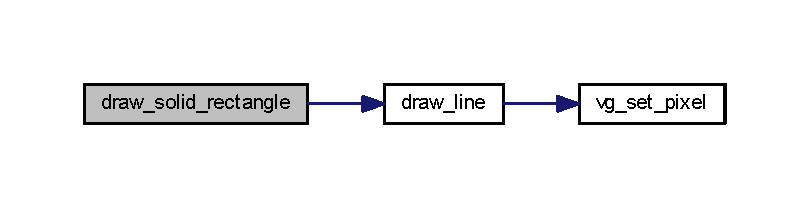
\includegraphics[width=350pt]{group__video__gr_ga021afd3327df962eafa769b82ed8e9a2_cgraph}
\end{center}
\end{figure}


\hypertarget{group__video__gr_ga62a06f3a0dc2bfe74941b60f3f0e4294}{}\index{video\+\_\+gr@{video\+\_\+gr}!get\+H\+R\+E\+S@{get\+H\+R\+E\+S}}
\index{get\+H\+R\+E\+S@{get\+H\+R\+E\+S}!video\+\_\+gr@{video\+\_\+gr}}
\subsubsection[{get\+H\+R\+E\+S}]{\setlength{\rightskip}{0pt plus 5cm}unsigned get\+H\+R\+E\+S (
\begin{DoxyParamCaption}
{}
\end{DoxyParamCaption}
)}\label{group__video__gr_ga62a06f3a0dc2bfe74941b60f3f0e4294}
Returns horizontal resolution of the screen 

Definition at line 38 of file video\+\_\+gr.\+c.

\hypertarget{group__video__gr_ga200a747d2cbe6ff688b650fa5972dcec}{}\index{video\+\_\+gr@{video\+\_\+gr}!get\+V\+R\+E\+S@{get\+V\+R\+E\+S}}
\index{get\+V\+R\+E\+S@{get\+V\+R\+E\+S}!video\+\_\+gr@{video\+\_\+gr}}
\subsubsection[{get\+V\+R\+E\+S}]{\setlength{\rightskip}{0pt plus 5cm}unsigned get\+V\+R\+E\+S (
\begin{DoxyParamCaption}
{}
\end{DoxyParamCaption}
)}\label{group__video__gr_ga200a747d2cbe6ff688b650fa5972dcec}
Returns vertical resolution of the screen 

Definition at line 43 of file video\+\_\+gr.\+c.

\hypertarget{group__video__gr_ga8ef5b4814293ba5d60d1d9cfaa648680}{}\index{video\+\_\+gr@{video\+\_\+gr}!test\+\_\+controller@{test\+\_\+controller}}
\index{test\+\_\+controller@{test\+\_\+controller}!video\+\_\+gr@{video\+\_\+gr}}
\subsubsection[{test\+\_\+controller}]{\setlength{\rightskip}{0pt plus 5cm}int test\+\_\+controller (
\begin{DoxyParamCaption}
{}
\end{DoxyParamCaption}
)}\label{group__video__gr_ga8ef5b4814293ba5d60d1d9cfaa648680}


Definition at line 136 of file test5.\+c.



Here is the call graph for this function\+:\nopagebreak
\begin{figure}[H]
\begin{center}
\leavevmode
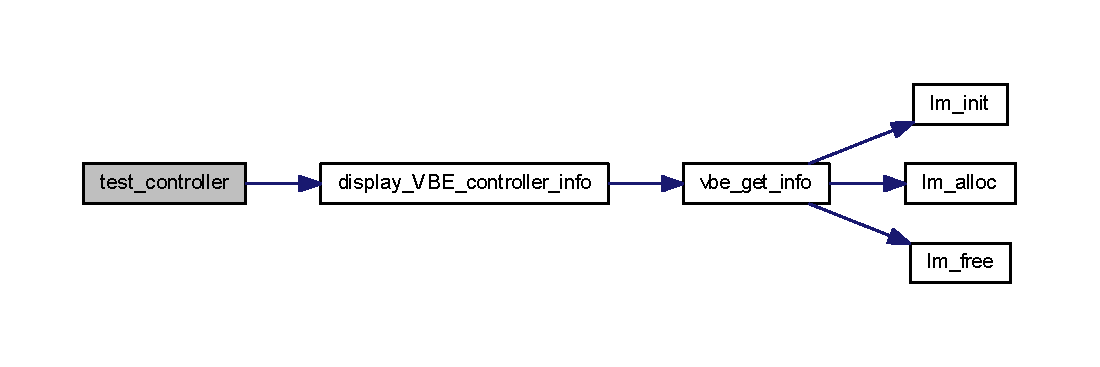
\includegraphics[width=350pt]{group__video__gr_ga8ef5b4814293ba5d60d1d9cfaa648680_cgraph}
\end{center}
\end{figure}


\hypertarget{group__video__gr_ga6e39c6cb8202eb0246f40572deef605a}{}\index{video\+\_\+gr@{video\+\_\+gr}!test\+\_\+init@{test\+\_\+init}}
\index{test\+\_\+init@{test\+\_\+init}!video\+\_\+gr@{video\+\_\+gr}}
\subsubsection[{test\+\_\+init}]{\setlength{\rightskip}{0pt plus 5cm}void$\ast$ test\+\_\+init (
\begin{DoxyParamCaption}
\item[{unsigned short}]{mode, }
\item[{unsigned short}]{delay}
\end{DoxyParamCaption}
)}\label{group__video__gr_ga6e39c6cb8202eb0246f40572deef605a}


Tests initialization of video card in graphics mode. 

Uses the V\+B\+E I\+N\+T 0x10 interface to set the desired graphics mode, and resets Minix\textquotesingle{}s default text mode after a short delay. Before exiting, displays on the console the physical address of V\+R\+A\+M in the input graphics mode.


\begin{DoxyParams}{Parameters}
{\em mode} & 16-\/bit V\+B\+E mode to set \\
\hline
{\em delay} & delay in seconds after which returns to text mode \\
\hline
\end{DoxyParams}
\begin{DoxyReturn}{Returns}
Virtual address V\+R\+A\+M was mapped to. N\+U\+L\+L, upon failure. 
\end{DoxyReturn}


Definition at line 9 of file test5.\+c.



Here is the call graph for this function\+:\nopagebreak
\begin{figure}[H]
\begin{center}
\leavevmode
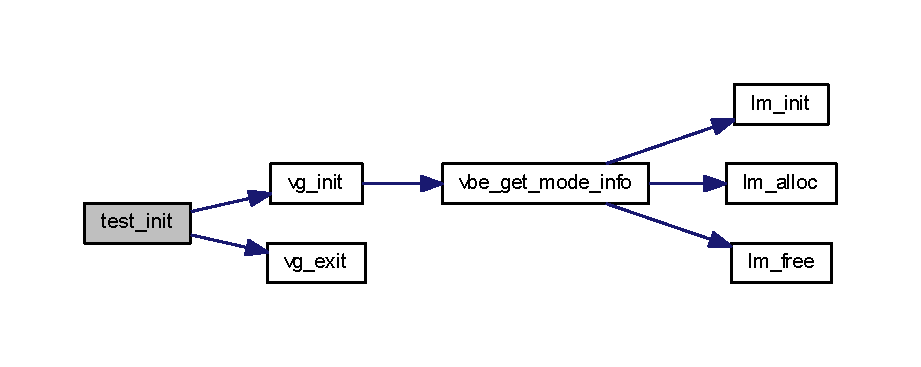
\includegraphics[width=350pt]{group__video__gr_ga6e39c6cb8202eb0246f40572deef605a_cgraph}
\end{center}
\end{figure}


\hypertarget{group__video__gr_gaddb118e00aa3152b6b6445f77a95b189}{}\index{video\+\_\+gr@{video\+\_\+gr}!test\+\_\+line@{test\+\_\+line}}
\index{test\+\_\+line@{test\+\_\+line}!video\+\_\+gr@{video\+\_\+gr}}
\subsubsection[{test\+\_\+line}]{\setlength{\rightskip}{0pt plus 5cm}int test\+\_\+line (
\begin{DoxyParamCaption}
\item[{unsigned short}]{xi, }
\item[{unsigned short}]{yi, }
\item[{unsigned short}]{xf, }
\item[{unsigned short}]{yf, }
\item[{unsigned long}]{color}
\end{DoxyParamCaption}
)}\label{group__video__gr_gaddb118e00aa3152b6b6445f77a95b189}


Tests drawing a line segment with specifed end points and color. 

Tests drawing a line segment with the specified end points and the input color, by writing to V\+R\+A\+M in video mode 0x105


\begin{DoxyParams}{Parameters}
{\em xi} & horizontal coordinate of \char`\"{}first\char`\"{} endpoint, starts at 0 (leftmost pixel) \\
\hline
{\em yi} & vertical coordinate of \char`\"{}first\char`\"{} endpoint, starts at 0 (top pixel) \\
\hline
{\em xf} & horizontal coordinate of \char`\"{}last\char`\"{} endpoint, starts at 0 (leftmost pixel) \\
\hline
{\em yf} & vertical coordinate of \char`\"{}last\char`\"{} endpoint, starts at 0 (top pixel) \\
\hline
{\em color} & color of the line segment to draw \\
\hline
\end{DoxyParams}
\begin{DoxyReturn}{Returns}
0 upon success, non-\/zero upon failure 
\end{DoxyReturn}


Definition at line 31 of file test5.\+c.



Here is the call graph for this function\+:\nopagebreak
\begin{figure}[H]
\begin{center}
\leavevmode
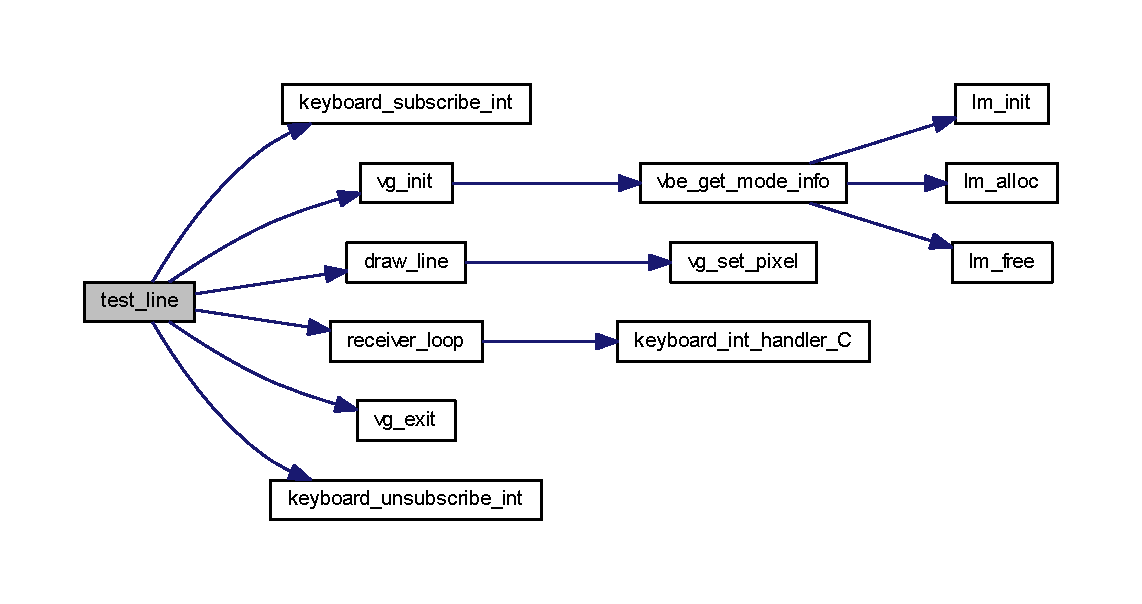
\includegraphics[width=350pt]{group__video__gr_gaddb118e00aa3152b6b6445f77a95b189_cgraph}
\end{center}
\end{figure}


\hypertarget{group__video__gr_ga07be3b073d0119c528934e24c0312c87}{}\index{video\+\_\+gr@{video\+\_\+gr}!test\+\_\+move@{test\+\_\+move}}
\index{test\+\_\+move@{test\+\_\+move}!video\+\_\+gr@{video\+\_\+gr}}
\subsubsection[{test\+\_\+move}]{\setlength{\rightskip}{0pt plus 5cm}int test\+\_\+move (
\begin{DoxyParamCaption}
\item[{unsigned short}]{xi, }
\item[{unsigned short}]{yi, }
\item[{char $\ast$}]{xpm\mbox{[}$\,$\mbox{]}, }
\item[{unsigned short}]{hor, }
\item[{short}]{delta, }
\item[{unsigned short}]{time}
\end{DoxyParamCaption}
)}\label{group__video__gr_ga07be3b073d0119c528934e24c0312c87}


Tests moving sprite on the screen along horizontal/vertical axes. 

Tests moving a X\+P\+M on the screen along horizontal/vertical axes, at the specified speed, in video mode 0x105


\begin{DoxyParams}{Parameters}
{\em xi} & horizontal coordinate of upper-\/left corner, starts at 0 (leftmost pixel) \\
\hline
{\em yi} & vertical coordinate of upper-\/left corner, starts at 0 (top pixel) \\
\hline
{\em xpm} & array with X\+P\+M (assuming indexed color mode) \\
\hline
{\em hor} & whether the movement is in the horizontal direction (!= 0) or in the vertical direction (== 0) \\
\hline
{\em delta} & movement in along specified direction in pixels \\
\hline
{\em time} & duration in seconds of the movement \\
\hline
\end{DoxyParams}
\begin{DoxyReturn}{Returns}
0 upon success, non-\/zero upon failure 
\end{DoxyReturn}


Definition at line 66 of file test5.\+c.



Here is the call graph for this function\+:\nopagebreak
\begin{figure}[H]
\begin{center}
\leavevmode
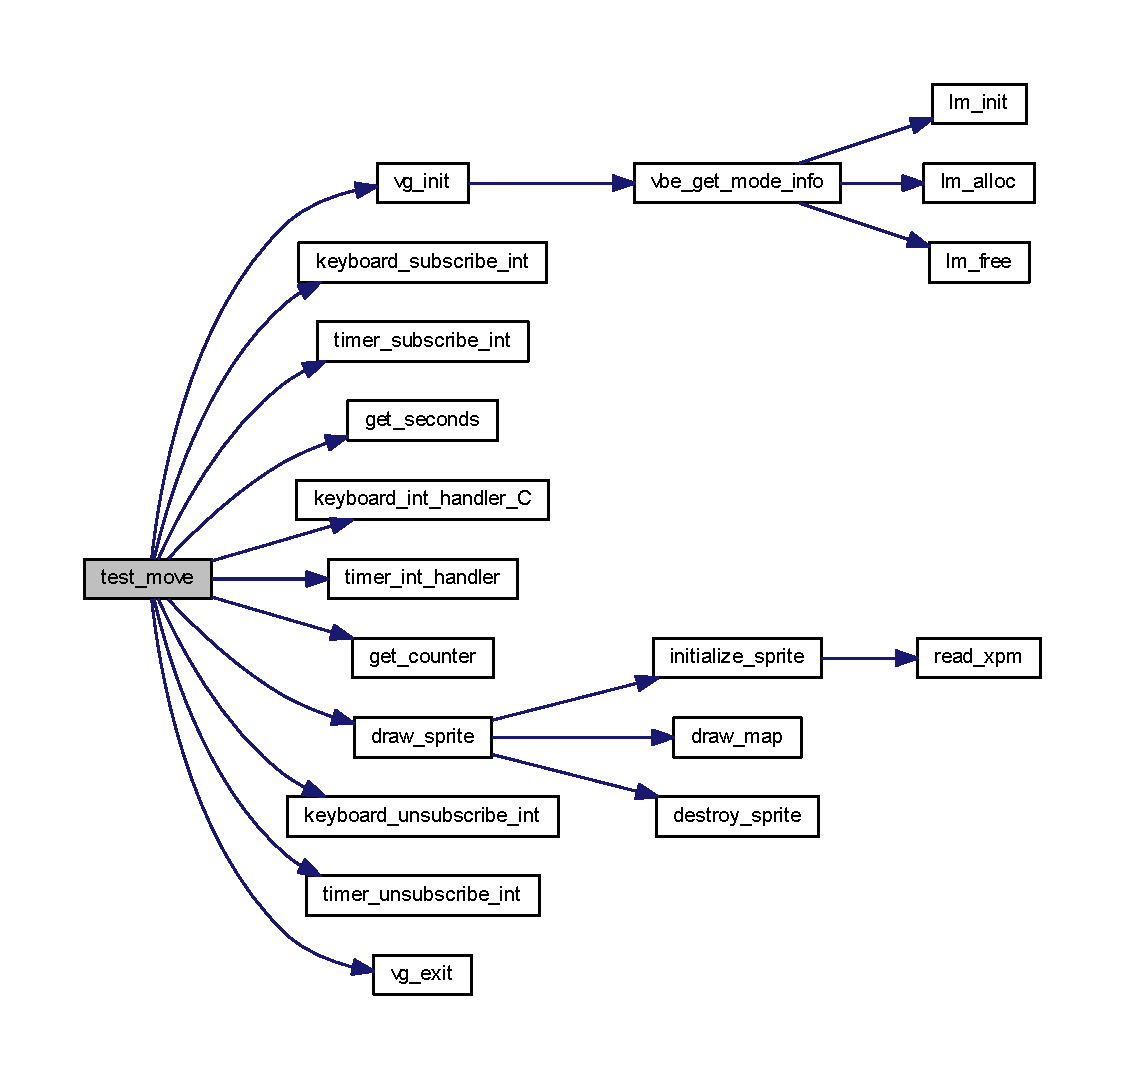
\includegraphics[width=350pt]{group__video__gr_ga07be3b073d0119c528934e24c0312c87_cgraph}
\end{center}
\end{figure}


\hypertarget{group__video__gr_ga41ec579061f8d7e2dc435e94efaac75e}{}\index{video\+\_\+gr@{video\+\_\+gr}!test\+\_\+square@{test\+\_\+square}}
\index{test\+\_\+square@{test\+\_\+square}!video\+\_\+gr@{video\+\_\+gr}}
\subsubsection[{test\+\_\+square}]{\setlength{\rightskip}{0pt plus 5cm}int test\+\_\+square (
\begin{DoxyParamCaption}
\item[{unsigned short}]{x, }
\item[{unsigned short}]{y, }
\item[{unsigned short}]{size, }
\item[{unsigned long}]{color}
\end{DoxyParamCaption}
)}\label{group__video__gr_ga41ec579061f8d7e2dc435e94efaac75e}


Tests drawing a square with a given color. 

Tests drawing a square with the specified size and color, at the specified coordinates (which specify the upper left corner (U\+L\+C)) in video mode 0x105


\begin{DoxyParams}{Parameters}
{\em x} & horizontal coordinate of U\+L\+C, starts at 0 (leftmost pixel) \\
\hline
{\em y} & vertical coordinate of U\+L\+C, starts at 0 (top pixel) \\
\hline
{\em size} & of each side in pixels \\
\hline
{\em color} & color to set the pixel \\
\hline
\end{DoxyParams}
\begin{DoxyReturn}{Returns}
0 on success, non-\/zero otherwise 
\end{DoxyReturn}


Definition at line 17 of file test5.\+c.



Here is the call graph for this function\+:\nopagebreak
\begin{figure}[H]
\begin{center}
\leavevmode
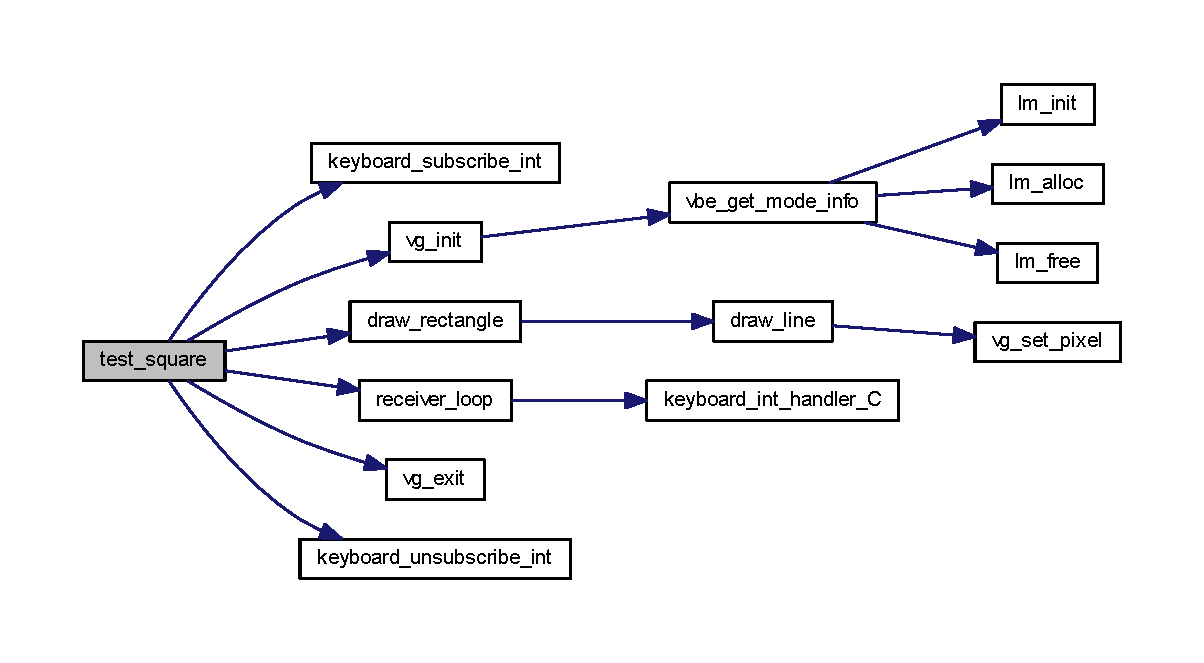
\includegraphics[width=350pt]{group__video__gr_ga41ec579061f8d7e2dc435e94efaac75e_cgraph}
\end{center}
\end{figure}


\hypertarget{group__video__gr_ga4dfc8ee51e363da1ecfe9fba1210bdb2}{}\index{video\+\_\+gr@{video\+\_\+gr}!test\+\_\+xpm@{test\+\_\+xpm}}
\index{test\+\_\+xpm@{test\+\_\+xpm}!video\+\_\+gr@{video\+\_\+gr}}
\subsubsection[{test\+\_\+xpm}]{\setlength{\rightskip}{0pt plus 5cm}int test\+\_\+xpm (
\begin{DoxyParamCaption}
\item[{unsigned short}]{xi, }
\item[{unsigned short}]{yi, }
\item[{char $\ast$}]{xpm\mbox{[}$\,$\mbox{]}}
\end{DoxyParamCaption}
)}\label{group__video__gr_ga4dfc8ee51e363da1ecfe9fba1210bdb2}


Tests drawing X\+P\+M on the screen at specified coordinates. 

Tests drawing a sprite from an X\+P\+M on the screen at specified coordinates by writing to V\+R\+A\+M in video mode 0x105


\begin{DoxyParams}{Parameters}
{\em xi} & horizontal coordinate of upper-\/left corner, starts at 0 (leftmost pixel) \\
\hline
{\em yi} & vertical coordinate of upper-\/left corner, starts at 0 (top pixel) \\
\hline
{\em xpm} & array with X\+P\+M (assuming indexed color mode) \\
\hline
\end{DoxyParams}
\begin{DoxyReturn}{Returns}
0 upon success, non-\/zero upon failure 
\end{DoxyReturn}


Definition at line 48 of file test5.\+c.



Here is the call graph for this function\+:\nopagebreak
\begin{figure}[H]
\begin{center}
\leavevmode
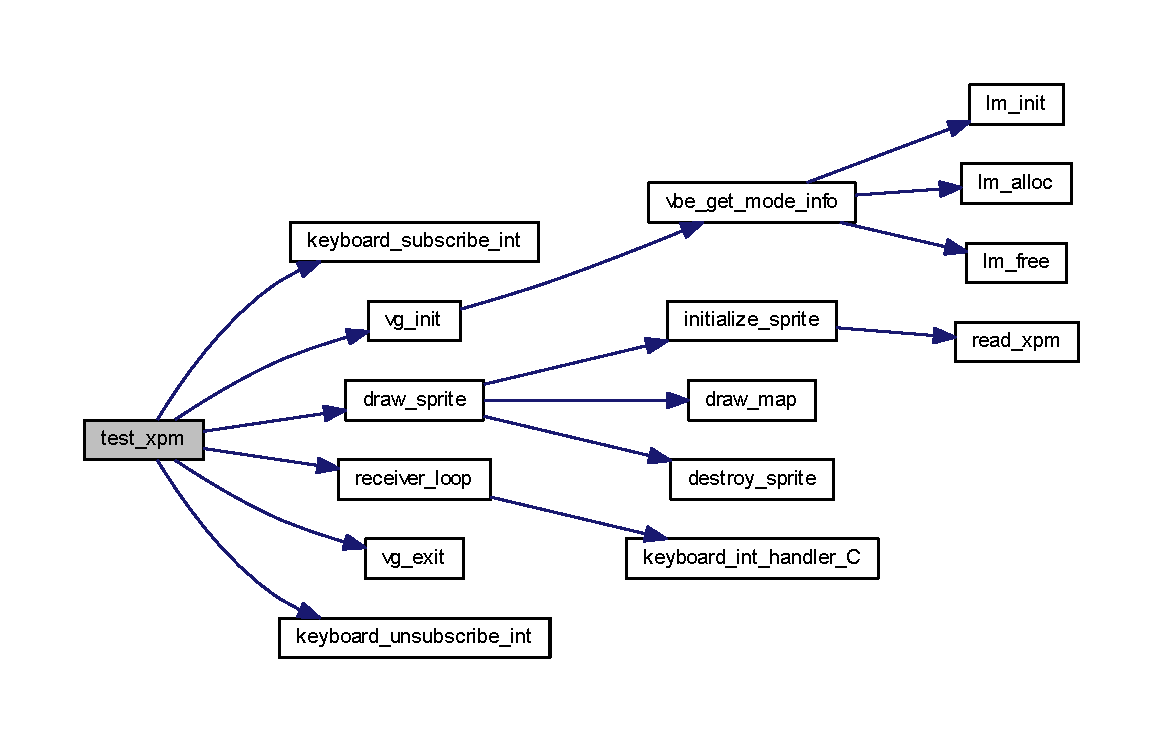
\includegraphics[width=350pt]{group__video__gr_ga4dfc8ee51e363da1ecfe9fba1210bdb2_cgraph}
\end{center}
\end{figure}


\hypertarget{group__video__gr_ga42f593e6656f1a978315aff02b1bcebf}{}\index{video\+\_\+gr@{video\+\_\+gr}!vg\+\_\+exit@{vg\+\_\+exit}}
\index{vg\+\_\+exit@{vg\+\_\+exit}!video\+\_\+gr@{video\+\_\+gr}}
\subsubsection[{vg\+\_\+exit}]{\setlength{\rightskip}{0pt plus 5cm}int vg\+\_\+exit (
\begin{DoxyParamCaption}
\item[{void}]{}
\end{DoxyParamCaption}
)}\label{group__video__gr_ga42f593e6656f1a978315aff02b1bcebf}


Returns to default Minix 3 text mode (0x03\+: 25 x 80, 16 colors) 

\begin{DoxyReturn}{Returns}
0 upon success, non-\/zero upon failure 
\end{DoxyReturn}


Definition at line 291 of file video\+\_\+gr.\+c.

\hypertarget{group__video__gr_ga225408a4d744af43112aa410a92d303b}{}\index{video\+\_\+gr@{video\+\_\+gr}!vg\+\_\+fill@{vg\+\_\+fill}}
\index{vg\+\_\+fill@{vg\+\_\+fill}!video\+\_\+gr@{video\+\_\+gr}}
\subsubsection[{vg\+\_\+fill}]{\setlength{\rightskip}{0pt plus 5cm}int vg\+\_\+fill (
\begin{DoxyParamCaption}
\item[{unsigned long}]{color}
\end{DoxyParamCaption}
)}\label{group__video__gr_ga225408a4d744af43112aa410a92d303b}


Definition at line 107 of file video\+\_\+gr.\+c.

\hypertarget{group__video__gr_gacef21667c79365d57a084bed994c2189}{}\index{video\+\_\+gr@{video\+\_\+gr}!vg\+\_\+init@{vg\+\_\+init}}
\index{vg\+\_\+init@{vg\+\_\+init}!video\+\_\+gr@{video\+\_\+gr}}
\subsubsection[{vg\+\_\+init}]{\setlength{\rightskip}{0pt plus 5cm}void$\ast$ vg\+\_\+init (
\begin{DoxyParamCaption}
\item[{unsigned short}]{mode}
\end{DoxyParamCaption}
)}\label{group__video__gr_gacef21667c79365d57a084bed994c2189}


Initializes the video module in graphics mode. 

Uses the V\+B\+E I\+N\+T 0x10 interface to set the desired graphics mode, maps V\+R\+A\+M to the process\textquotesingle{} address space and initializes static global variables with the resolution of the screen, and the number of colors


\begin{DoxyParams}{Parameters}
{\em mode} & 16-\/bit V\+B\+E mode to set \\
\hline
\end{DoxyParams}
\begin{DoxyReturn}{Returns}
Virtual address V\+R\+A\+M was mapped to. N\+U\+L\+L, upon failure. 
\end{DoxyReturn}


Definition at line 52 of file video\+\_\+gr.\+c.



Here is the call graph for this function\+:\nopagebreak
\begin{figure}[H]
\begin{center}
\leavevmode
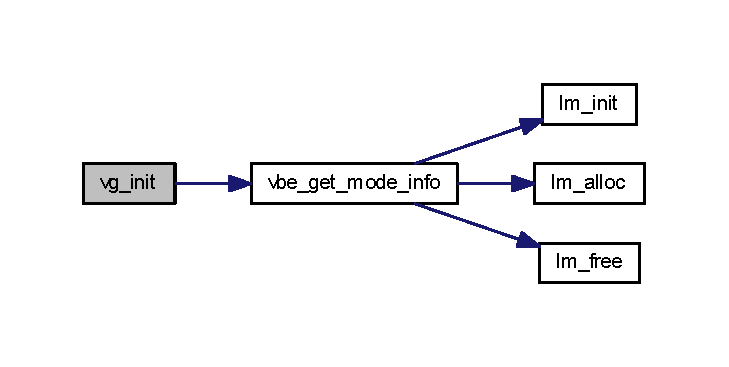
\includegraphics[width=350pt]{group__video__gr_gacef21667c79365d57a084bed994c2189_cgraph}
\end{center}
\end{figure}



\hypertarget{group__timer}{}\section{timer}
\label{group__timer}\index{timer@{timer}}
\subsection*{Functions}
\begin{DoxyCompactItemize}
\item 
int \hyperlink{group__timer_gada4efbb5c88275795526fc45f0814aa3}{timer\+\_\+set\+\_\+square} (unsigned long timer, unsigned long freq)
\begin{DoxyCompactList}\small\item\em Configures a timer to generate a square wave. \end{DoxyCompactList}\item 
int \hyperlink{group__timer_ga4c5d9f47323eda494cfd826f6d62eec9}{timer\+\_\+subscribe\+\_\+int} (void)
\begin{DoxyCompactList}\small\item\em Subscribes and enables Timer 0 interrupts. \end{DoxyCompactList}\item 
int \hyperlink{group__timer_gab9eea51549744bca5c5c923b388bb4ee}{timer\+\_\+unsubscribe\+\_\+int} ()
\begin{DoxyCompactList}\small\item\em Unsubscribes Timer 0 interrupts. \end{DoxyCompactList}\item 
void \hyperlink{group__timer_ga10fc9c867b15c7da6649311c9987cd17}{timer\+\_\+int\+\_\+handler} ()
\begin{DoxyCompactList}\small\item\em Timer 0 interrupt handler. \end{DoxyCompactList}\item 
int \hyperlink{group__timer_ga8eb3357bc05265afc4bea5bbbb480a53}{timer\+\_\+get\+\_\+conf} (unsigned long timer, unsigned char $\ast$st)
\begin{DoxyCompactList}\small\item\em Reads the input timer configuration via read-\/back command. \end{DoxyCompactList}\item 
int \hyperlink{group__timer_ga9ca64a3f3f048936d961d656d6829200}{timer\+\_\+display\+\_\+conf} (unsigned char conf)
\begin{DoxyCompactList}\small\item\em Shows timer configuration. \end{DoxyCompactList}\item 
int \hyperlink{group__timer_ga2e596aede5a7bfc4a6f4382779bf0d7d}{timer\+\_\+test\+\_\+square} (unsigned long freq)
\begin{DoxyCompactList}\small\item\em Tests programming timer in square wave mode. \end{DoxyCompactList}\item 
int \hyperlink{group__timer_ga459859709b7cc1ee37899fa48cce6a6e}{timer\+\_\+test\+\_\+int} (unsigned long time)
\begin{DoxyCompactList}\small\item\em Tests Timer 0 interrupt handling. \end{DoxyCompactList}\item 
int \hyperlink{group__timer_ga363e72d1c055d859746cb3305a68af6d}{timer\+\_\+test\+\_\+config} (unsigned long timer)
\begin{DoxyCompactList}\small\item\em Tests display of timer config. \end{DoxyCompactList}\end{DoxyCompactItemize}


\subsection{Detailed Description}
Functions for using the i8254 timers 

\subsection{Function Documentation}
\hypertarget{group__timer_ga9ca64a3f3f048936d961d656d6829200}{}\index{timer@{timer}!timer\+\_\+display\+\_\+conf@{timer\+\_\+display\+\_\+conf}}
\index{timer\+\_\+display\+\_\+conf@{timer\+\_\+display\+\_\+conf}!timer@{timer}}
\subsubsection[{timer\+\_\+display\+\_\+conf}]{\setlength{\rightskip}{0pt plus 5cm}int timer\+\_\+display\+\_\+conf (
\begin{DoxyParamCaption}
\item[{unsigned char}]{conf}
\end{DoxyParamCaption}
)}\label{group__timer_ga9ca64a3f3f048936d961d656d6829200}


Shows timer configuration. 

Displays in a human friendly way, the configuration of a timer as read via the read-\/back command, by providing the values (and meanings) of the different components of a timer configuration


\begin{DoxyParams}{Parameters}
{\em conf} & configuration to display in human friendly way \\
\hline
\end{DoxyParams}
\begin{DoxyReturn}{Returns}
Return 0 upon success and non-\/zero otherwise 
\end{DoxyReturn}


Definition at line 80 of file timer.\+c.

\hypertarget{group__timer_ga8eb3357bc05265afc4bea5bbbb480a53}{}\index{timer@{timer}!timer\+\_\+get\+\_\+conf@{timer\+\_\+get\+\_\+conf}}
\index{timer\+\_\+get\+\_\+conf@{timer\+\_\+get\+\_\+conf}!timer@{timer}}
\subsubsection[{timer\+\_\+get\+\_\+conf}]{\setlength{\rightskip}{0pt plus 5cm}int timer\+\_\+get\+\_\+conf (
\begin{DoxyParamCaption}
\item[{unsigned long}]{timer, }
\item[{unsigned char $\ast$}]{st}
\end{DoxyParamCaption}
)}\label{group__timer_ga8eb3357bc05265afc4bea5bbbb480a53}


Reads the input timer configuration via read-\/back command. 


\begin{DoxyParams}{Parameters}
{\em timer} & Timer whose config to read (Ranges from 0 to 2) \\
\hline
{\em st} & Address of memory position to be filled with the timer config \\
\hline
\end{DoxyParams}
\begin{DoxyReturn}{Returns}
Return 0 upon success and non-\/zero otherwise 
\end{DoxyReturn}


Definition at line 65 of file timer.\+c.

\hypertarget{group__timer_ga10fc9c867b15c7da6649311c9987cd17}{}\index{timer@{timer}!timer\+\_\+int\+\_\+handler@{timer\+\_\+int\+\_\+handler}}
\index{timer\+\_\+int\+\_\+handler@{timer\+\_\+int\+\_\+handler}!timer@{timer}}
\subsubsection[{timer\+\_\+int\+\_\+handler}]{\setlength{\rightskip}{0pt plus 5cm}void timer\+\_\+int\+\_\+handler (
\begin{DoxyParamCaption}
{}
\end{DoxyParamCaption}
)}\label{group__timer_ga10fc9c867b15c7da6649311c9987cd17}


Timer 0 interrupt handler. 

Increments counter 

Definition at line 39 of file timer.\+c.

\hypertarget{group__timer_gada4efbb5c88275795526fc45f0814aa3}{}\index{timer@{timer}!timer\+\_\+set\+\_\+square@{timer\+\_\+set\+\_\+square}}
\index{timer\+\_\+set\+\_\+square@{timer\+\_\+set\+\_\+square}!timer@{timer}}
\subsubsection[{timer\+\_\+set\+\_\+square}]{\setlength{\rightskip}{0pt plus 5cm}int timer\+\_\+set\+\_\+square (
\begin{DoxyParamCaption}
\item[{unsigned long}]{timer, }
\item[{unsigned long}]{freq}
\end{DoxyParamCaption}
)}\label{group__timer_gada4efbb5c88275795526fc45f0814aa3}


Configures a timer to generate a square wave. 

Does not change the L\+S\+B (B\+C\+D/binary) of the timer\textquotesingle{}s control word.


\begin{DoxyParams}{Parameters}
{\em timer} & Timer to configure. (Ranges from 0 to 2) \\
\hline
{\em freq} & Frequency of the square wave to generate \\
\hline
\end{DoxyParams}
\begin{DoxyReturn}{Returns}
Return 0 upon success and non-\/zero otherwise 
\end{DoxyReturn}


Definition at line 7 of file timer.\+c.



Here is the call graph for this function\+:\nopagebreak
\begin{figure}[H]
\begin{center}
\leavevmode
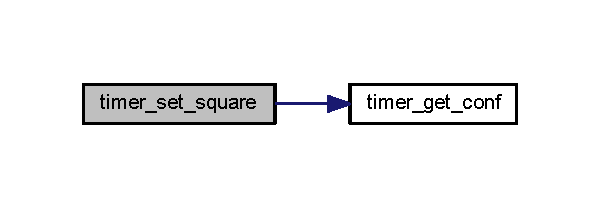
\includegraphics[width=288pt]{group__timer_gada4efbb5c88275795526fc45f0814aa3_cgraph}
\end{center}
\end{figure}


\hypertarget{group__timer_ga4c5d9f47323eda494cfd826f6d62eec9}{}\index{timer@{timer}!timer\+\_\+subscribe\+\_\+int@{timer\+\_\+subscribe\+\_\+int}}
\index{timer\+\_\+subscribe\+\_\+int@{timer\+\_\+subscribe\+\_\+int}!timer@{timer}}
\subsubsection[{timer\+\_\+subscribe\+\_\+int}]{\setlength{\rightskip}{0pt plus 5cm}int timer\+\_\+subscribe\+\_\+int (
\begin{DoxyParamCaption}
\item[{void}]{}
\end{DoxyParamCaption}
)}\label{group__timer_ga4c5d9f47323eda494cfd826f6d62eec9}


Subscribes and enables Timer 0 interrupts. 

\begin{DoxyReturn}{Returns}
Returns bit order in interrupt mask; negative value on failure 
\end{DoxyReturn}


Definition at line 27 of file timer.\+c.

\hypertarget{group__timer_ga363e72d1c055d859746cb3305a68af6d}{}\index{timer@{timer}!timer\+\_\+test\+\_\+config@{timer\+\_\+test\+\_\+config}}
\index{timer\+\_\+test\+\_\+config@{timer\+\_\+test\+\_\+config}!timer@{timer}}
\subsubsection[{timer\+\_\+test\+\_\+config}]{\setlength{\rightskip}{0pt plus 5cm}int timer\+\_\+test\+\_\+config (
\begin{DoxyParamCaption}
\item[{unsigned long}]{timer}
\end{DoxyParamCaption}
)}\label{group__timer_ga363e72d1c055d859746cb3305a68af6d}


Tests display of timer config. 

Just calls \hyperlink{group__timer_ga8eb3357bc05265afc4bea5bbbb480a53}{timer\+\_\+get\+\_\+conf()} followed by \hyperlink{group__timer_ga9ca64a3f3f048936d961d656d6829200}{timer\+\_\+display\+\_\+conf()}


\begin{DoxyParams}{Parameters}
{\em timer} & Timer whose config to read (Ranges from 0 to 2) \\
\hline
\end{DoxyParams}
\begin{DoxyReturn}{Returns}
Return 0 upon success and non-\/zero otherwise 
\end{DoxyReturn}


Definition at line 143 of file timer.\+c.



Here is the call graph for this function\+:\nopagebreak
\begin{figure}[H]
\begin{center}
\leavevmode
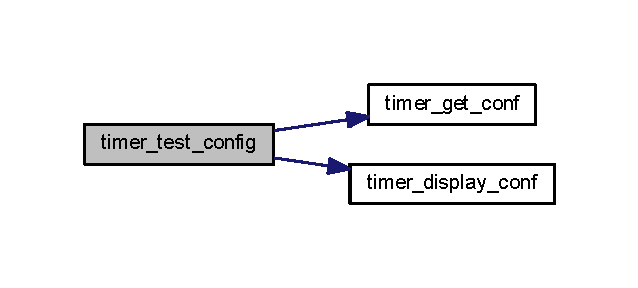
\includegraphics[width=306pt]{group__timer_ga363e72d1c055d859746cb3305a68af6d_cgraph}
\end{center}
\end{figure}


\hypertarget{group__timer_ga459859709b7cc1ee37899fa48cce6a6e}{}\index{timer@{timer}!timer\+\_\+test\+\_\+int@{timer\+\_\+test\+\_\+int}}
\index{timer\+\_\+test\+\_\+int@{timer\+\_\+test\+\_\+int}!timer@{timer}}
\subsubsection[{timer\+\_\+test\+\_\+int}]{\setlength{\rightskip}{0pt plus 5cm}int timer\+\_\+test\+\_\+int (
\begin{DoxyParamCaption}
\item[{unsigned long}]{time}
\end{DoxyParamCaption}
)}\label{group__timer_ga459859709b7cc1ee37899fa48cce6a6e}


Tests Timer 0 interrupt handling. 

Subscribes Timer 0 interrupts and prints a message once per second for the specified time interval


\begin{DoxyParams}{Parameters}
{\em time} & Length of time interval while interrupts are subscribed \\
\hline
\end{DoxyParams}
\begin{DoxyReturn}{Returns}
Return 0 upon success and non-\/zero otherwise 
\end{DoxyReturn}


Definition at line 107 of file timer.\+c.



Here is the call graph for this function\+:\nopagebreak
\begin{figure}[H]
\begin{center}
\leavevmode
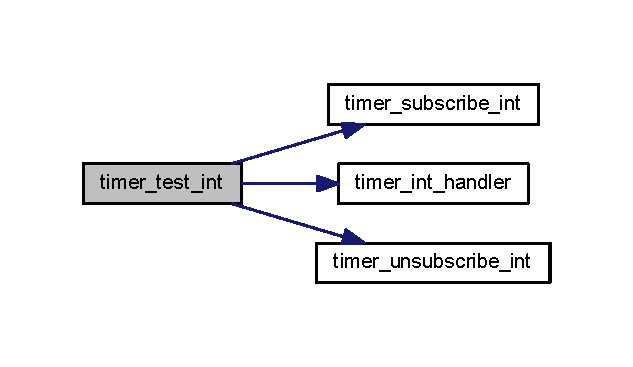
\includegraphics[width=304pt]{group__timer_ga459859709b7cc1ee37899fa48cce6a6e_cgraph}
\end{center}
\end{figure}


\hypertarget{group__timer_ga2e596aede5a7bfc4a6f4382779bf0d7d}{}\index{timer@{timer}!timer\+\_\+test\+\_\+square@{timer\+\_\+test\+\_\+square}}
\index{timer\+\_\+test\+\_\+square@{timer\+\_\+test\+\_\+square}!timer@{timer}}
\subsubsection[{timer\+\_\+test\+\_\+square}]{\setlength{\rightskip}{0pt plus 5cm}int timer\+\_\+test\+\_\+square (
\begin{DoxyParamCaption}
\item[{unsigned long}]{freq}
\end{DoxyParamCaption}
)}\label{group__timer_ga2e596aede5a7bfc4a6f4382779bf0d7d}


Tests programming timer in square wave mode. 

Programs Timer 0 to generate square mode with input frequency


\begin{DoxyParams}{Parameters}
{\em freq} & Frequency of square wave to generate \\
\hline
\end{DoxyParams}
\begin{DoxyReturn}{Returns}
Return 0 upon success and non-\/zero otherwise 
\end{DoxyReturn}


Definition at line 102 of file timer.\+c.



Here is the call graph for this function\+:\nopagebreak
\begin{figure}[H]
\begin{center}
\leavevmode
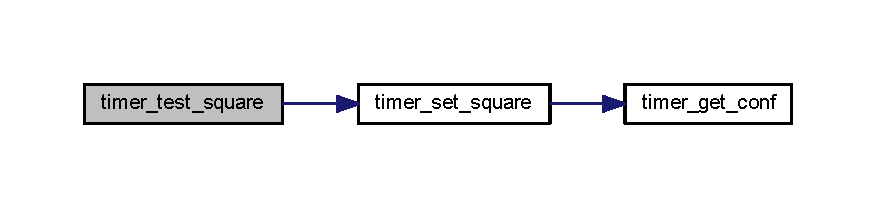
\includegraphics[width=350pt]{group__timer_ga2e596aede5a7bfc4a6f4382779bf0d7d_cgraph}
\end{center}
\end{figure}


\hypertarget{group__timer_gab9eea51549744bca5c5c923b388bb4ee}{}\index{timer@{timer}!timer\+\_\+unsubscribe\+\_\+int@{timer\+\_\+unsubscribe\+\_\+int}}
\index{timer\+\_\+unsubscribe\+\_\+int@{timer\+\_\+unsubscribe\+\_\+int}!timer@{timer}}
\subsubsection[{timer\+\_\+unsubscribe\+\_\+int}]{\setlength{\rightskip}{0pt plus 5cm}int timer\+\_\+unsubscribe\+\_\+int (
\begin{DoxyParamCaption}
{}
\end{DoxyParamCaption}
)}\label{group__timer_gab9eea51549744bca5c5c923b388bb4ee}


Unsubscribes Timer 0 interrupts. 

\begin{DoxyReturn}{Returns}
Return 0 upon success and non-\/zero otherwise 
\end{DoxyReturn}


Definition at line 34 of file timer.\+c.


\hypertarget{group__vbe}{}\section{vbe}
\label{group__vbe}\index{vbe@{vbe}}
\subsection*{Classes}
\begin{DoxyCompactItemize}
\item 
struct \hyperlink{struct____attribute____}{\+\_\+\+\_\+attribute\+\_\+\+\_\+}
\end{DoxyCompactItemize}
\subsection*{Functions}
\begin{DoxyCompactItemize}
\item 
int \hyperlink{group__vbe_ga4ef3234e41f2050bc094a22049b69e45}{vbe\+\_\+get\+\_\+mode\+\_\+info} (unsigned short mode, vbe\+\_\+mode\+\_\+info\+\_\+t $\ast$vmi\+\_\+p)
\begin{DoxyCompactList}\small\item\em Returns information on the input V\+B\+E mode, including screen dimensions, color depth and V\+R\+A\+M physical address. \end{DoxyCompactList}\end{DoxyCompactItemize}


\subsection{Detailed Description}
Functions related to the V\+B\+E standard 

\subsection{Function Documentation}
\hypertarget{group__vbe_ga4ef3234e41f2050bc094a22049b69e45}{}\index{vbe@{vbe}!vbe\+\_\+get\+\_\+mode\+\_\+info@{vbe\+\_\+get\+\_\+mode\+\_\+info}}
\index{vbe\+\_\+get\+\_\+mode\+\_\+info@{vbe\+\_\+get\+\_\+mode\+\_\+info}!vbe@{vbe}}
\subsubsection[{vbe\+\_\+get\+\_\+mode\+\_\+info}]{\setlength{\rightskip}{0pt plus 5cm}int vbe\+\_\+get\+\_\+mode\+\_\+info (
\begin{DoxyParamCaption}
\item[{unsigned short}]{mode, }
\item[{vbe\+\_\+mode\+\_\+info\+\_\+t $\ast$}]{vmi\+\_\+p}
\end{DoxyParamCaption}
)}\label{group__vbe_ga4ef3234e41f2050bc094a22049b69e45}


Returns information on the input V\+B\+E mode, including screen dimensions, color depth and V\+R\+A\+M physical address. 

Initializes unpacked vbe\+\_\+mode\+\_\+\+\_\+info\+\_\+t structure passed as an address with the information of the input mode, by calling V\+B\+E function 0x01 Return V\+B\+E Mode Information and unpacking the Mode\+Info\+Block struct returned by that function.


\begin{DoxyParams}{Parameters}
{\em mode} & mode whose information should be returned \\
\hline
{\em vmi\+\_\+p} & address of vbe\+\_\+mode\+\_\+info\+\_\+t structure to be initialized \\
\hline
\end{DoxyParams}
\begin{DoxyReturn}{Returns}
0 on success, non-\/zero otherwise 
\end{DoxyReturn}


Definition at line 15 of file vbe.\+c.



Here is the call graph for this function\+:\nopagebreak
\begin{figure}[H]
\begin{center}
\leavevmode
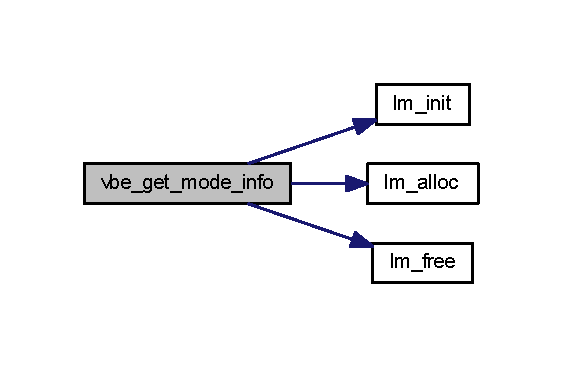
\includegraphics[width=270pt]{group__vbe_ga4ef3234e41f2050bc094a22049b69e45_cgraph}
\end{center}
\end{figure}



\chapter{Class Documentation}
\hypertarget{struct____attribute____}{}\section{\+\_\+\+\_\+attribute\+\_\+\+\_\+ Struct Reference}
\label{struct____attribute____}\index{\+\_\+\+\_\+attribute\+\_\+\+\_\+@{\+\_\+\+\_\+attribute\+\_\+\+\_\+}}


{\ttfamily \#include $<$vbe.\+h$>$}

\subsection*{Public Attributes}
\begin{DoxyCompactItemize}
\item 
uint32\+\_\+t \hyperlink{struct____attribute_____aae97bc03200134a557339f79aeeea94e}{Vbe\+Signature}
\item 
uint16\+\_\+t \hyperlink{struct____attribute_____ab50a7a6ed578c30d9411db043c0b34c9}{Vbe\+Version}
\item 
uint32\+\_\+t \hyperlink{struct____attribute_____acc74a7d7f3d3d90bc058f13f4d30a61c}{Oem\+String\+Ptr}
\item 
u8\+\_\+t \hyperlink{struct____attribute_____a22a17ae44df67e1ebae6eb2721b64279}{Capabilities} \mbox{[}4\mbox{]}
\item 
uint16\+\_\+t \hyperlink{struct____attribute_____a135a4de316befee6c1415c22e5636f15}{Video\+Mode\+Ptr} \mbox{[}2\mbox{]}
\item 
uint16\+\_\+t \hyperlink{struct____attribute_____a5659e88b961bf423d6385f315264e005}{Total\+Memory}
\item 
uint16\+\_\+t \hyperlink{struct____attribute_____abd3b5364844ce7019b91c129b5535f42}{Oem\+Software\+Rev}
\item 
uint32\+\_\+t \hyperlink{struct____attribute_____ad8741201b5c9013911dd092185d780b6}{Oem\+Vendor\+Name\+Ptr}
\item 
uint32\+\_\+t \hyperlink{struct____attribute_____a79d41d28ea7c0aa5c8f36e46c92ee2d0}{Oem\+Product\+Name\+Ptr}
\item 
uint32\+\_\+t \hyperlink{struct____attribute_____aa746b73bc137e19abbbac805a97594b9}{Oem\+Product\+Rev\+Ptr}
\item 
u8\+\_\+t \hyperlink{struct____attribute_____a7d9d8bf3e618f409748302e3d2484fe6}{Reserved} \mbox{[}222\mbox{]}
\item 
u8\+\_\+t \hyperlink{struct____attribute_____ac3f69bedeb0dc55c1ee1bd481a74b08e}{Oem\+Data} \mbox{[}256\mbox{]}
\item 
uint16\+\_\+t \hyperlink{struct____attribute_____a68ea99ad36679e583fa9674016e30903}{Mode\+Attributes}
\begin{DoxyCompactList}\small\item\em mode attributes \end{DoxyCompactList}\item 
uint8\+\_\+t \hyperlink{struct____attribute_____aeffe4dec59c5a757f65a97a66c812d3b}{Win\+A\+Attributes}
\begin{DoxyCompactList}\small\item\em window A attributes \end{DoxyCompactList}\item 
uint8\+\_\+t \hyperlink{struct____attribute_____ac9e21a3d7d22b24ed82be39f790b1408}{Win\+B\+Attributes}
\begin{DoxyCompactList}\small\item\em window B attributes \end{DoxyCompactList}\item 
uint16\+\_\+t \hyperlink{struct____attribute_____acc2114dbf039909e55cc3966abd3358d}{Win\+Granularity}
\begin{DoxyCompactList}\small\item\em window granularity \end{DoxyCompactList}\item 
uint16\+\_\+t \hyperlink{struct____attribute_____ad26e754fe362f3085c7ec4c0e5e75a6f}{Win\+Size}
\begin{DoxyCompactList}\small\item\em window size \end{DoxyCompactList}\item 
uint16\+\_\+t \hyperlink{struct____attribute_____a7cde26f911e3df97b7498ee139d8de12}{Win\+A\+Segment}
\begin{DoxyCompactList}\small\item\em window A start segment \end{DoxyCompactList}\item 
uint16\+\_\+t \hyperlink{struct____attribute_____a6dbaac9ee1cae36ca0c7b46559264b69}{Win\+B\+Segment}
\begin{DoxyCompactList}\small\item\em window B start segment \end{DoxyCompactList}\item 
phys\+\_\+bytes \hyperlink{struct____attribute_____aa211c2411f48f899b0bb0739ecef0b37}{Win\+Func\+Ptr}
\begin{DoxyCompactList}\small\item\em real mode/far pointer to window function \end{DoxyCompactList}\item 
uint16\+\_\+t \hyperlink{struct____attribute_____a3c9eb4b107ecee102c6e63f9054ede06}{Bytes\+Per\+Scan\+Line}
\begin{DoxyCompactList}\small\item\em bytes per scan line \end{DoxyCompactList}\item 
uint16\+\_\+t \hyperlink{struct____attribute_____abe48e2b29aa99e813a1447d22711f4f4}{X\+Resolution}
\begin{DoxyCompactList}\small\item\em horizontal resolution in pixels/characters \end{DoxyCompactList}\item 
uint16\+\_\+t \hyperlink{struct____attribute_____aa91385451d974d9c33978062e22d39e2}{Y\+Resolution}
\begin{DoxyCompactList}\small\item\em vertical resolution in pixels/characters \end{DoxyCompactList}\item 
uint8\+\_\+t \hyperlink{struct____attribute_____acac41a300563737d7849a92cd1d5c10b}{X\+Char\+Size}
\begin{DoxyCompactList}\small\item\em character cell width in pixels \end{DoxyCompactList}\item 
uint8\+\_\+t \hyperlink{struct____attribute_____acb93d86860efea5c87e3c2950f39123e}{Y\+Char\+Size}
\begin{DoxyCompactList}\small\item\em character cell height in pixels \end{DoxyCompactList}\item 
uint8\+\_\+t \hyperlink{struct____attribute_____ab1471d2f75e61117d65290da9070cf89}{Number\+Of\+Planes}
\begin{DoxyCompactList}\small\item\em number of memory planes \end{DoxyCompactList}\item 
uint8\+\_\+t \hyperlink{struct____attribute_____abd9c59af53589a54188bb57ada5c5f26}{Bits\+Per\+Pixel}
\begin{DoxyCompactList}\small\item\em bits per pixel \end{DoxyCompactList}\item 
uint8\+\_\+t \hyperlink{struct____attribute_____a59483378dd87414afcde6cb3ca93c2d8}{Number\+Of\+Banks}
\begin{DoxyCompactList}\small\item\em number of banks \end{DoxyCompactList}\item 
uint8\+\_\+t \hyperlink{struct____attribute_____a0fe34321b6dfba9e784fbbc649aa193a}{Memory\+Model}
\begin{DoxyCompactList}\small\item\em memory model type \end{DoxyCompactList}\item 
uint8\+\_\+t \hyperlink{struct____attribute_____aa1307567cbc12f9c5c724b7457be14ad}{Bank\+Size}
\begin{DoxyCompactList}\small\item\em bank size in K\+B \end{DoxyCompactList}\item 
uint8\+\_\+t \hyperlink{struct____attribute_____a988714bc16626547fbdc31f25dfa6470}{Number\+Of\+Image\+Pages}
\begin{DoxyCompactList}\small\item\em number of images \end{DoxyCompactList}\item 
uint8\+\_\+t \hyperlink{struct____attribute_____a8ace2dfe4814abc401442986ac8a5356}{Reserved1}
\begin{DoxyCompactList}\small\item\em reserved for page function \end{DoxyCompactList}\item 
uint8\+\_\+t \hyperlink{struct____attribute_____a9ffc14e11d6b1c80b63aba344292849e}{Red\+Mask\+Size}
\item 
uint8\+\_\+t \hyperlink{struct____attribute_____a8b5b2e458757061bce7e056f7f910dae}{Red\+Field\+Position}
\item 
uint8\+\_\+t \hyperlink{struct____attribute_____af69ef188a0f5d526ecd5f25a8d6336e3}{Green\+Mask\+Size}
\item 
uint8\+\_\+t \hyperlink{struct____attribute_____a44aab7c8026a131654e079837a95ba2b}{Green\+Field\+Position}
\item 
uint8\+\_\+t \hyperlink{struct____attribute_____ab5967602a79dcb7f0061195ffdaaa47a}{Blue\+Mask\+Size}
\item 
uint8\+\_\+t \hyperlink{struct____attribute_____ada852d5ed926757d24b5038a38e6292c}{Blue\+Field\+Position}
\item 
uint8\+\_\+t \hyperlink{struct____attribute_____a73862db83bdb9b6d31356af3cec7a5be}{Rsvd\+Mask\+Size}
\item 
uint8\+\_\+t \hyperlink{struct____attribute_____a61fb6dc07b7edbd8a3a94745336f256c}{Rsvd\+Field\+Position}
\item 
uint8\+\_\+t \hyperlink{struct____attribute_____a35fb3e1fc0dc9924bc52977b3a234f9f}{Direct\+Color\+Mode\+Info}
\item 
phys\+\_\+bytes \hyperlink{struct____attribute_____a852a4f68cfbabf08df197128e137bde6}{Phys\+Base\+Ptr}
\begin{DoxyCompactList}\small\item\em physical address for flat memory frame buffer \end{DoxyCompactList}\item 
uint8\+\_\+t \hyperlink{struct____attribute_____a534ebf7a2bdad17747cfc9cb6cc50c5c}{Reserved2} \mbox{[}4\mbox{]}
\begin{DoxyCompactList}\small\item\em Reserved -\/ always set to 0. \end{DoxyCompactList}\item 
uint8\+\_\+t \hyperlink{struct____attribute_____a9336499af9094522dbe1bfd4d43934a1}{Reserved3} \mbox{[}2\mbox{]}
\begin{DoxyCompactList}\small\item\em Reserved -\/ always set to 0. \end{DoxyCompactList}\item 
uint16\+\_\+t \hyperlink{struct____attribute_____af7036270c257deabc1ebd111faf3e3a5}{Lin\+Bytes\+Per\+Scan\+Line}
\item 
uint8\+\_\+t \hyperlink{struct____attribute_____ad5820084f2b821b85a635df8394f0d9e}{Bnk\+Number\+Of\+Image\+Pages}
\item 
uint8\+\_\+t \hyperlink{struct____attribute_____af9ba0d9902f5336bd9d044a9dee2ba42}{Lin\+Number\+Of\+Image\+Pages}
\item 
uint8\+\_\+t \hyperlink{struct____attribute_____a88a5ced225c9ef7ed6ffe33e5a39edc6}{Lin\+Red\+Mask\+Size}
\item 
uint8\+\_\+t \hyperlink{struct____attribute_____aec8d45f188ac9210b88216af83de847d}{Lin\+Red\+Field\+Position}
\item 
uint8\+\_\+t \hyperlink{struct____attribute_____a5768a84391f8a26d8a9bfd6a22d5e49d}{Lin\+Green\+Mask\+Size}
\item 
uint8\+\_\+t \hyperlink{struct____attribute_____a5571b1959950d520f2b45bb5549994e3}{Lin\+Green\+Field\+Position}
\item 
uint8\+\_\+t \hyperlink{struct____attribute_____aa2b79b8eed8d842e0db481fb1fbb9a06}{Lin\+Blue\+Mask\+Size}
\item 
uint8\+\_\+t \hyperlink{struct____attribute_____a99e6b6bdbda9f98f2823429dfd5b5685}{Lin\+Blue\+Field\+Position}
\item 
uint8\+\_\+t \hyperlink{struct____attribute_____a577b5892a22d06e230f528a62a472d1d}{Lin\+Rsvd\+Mask\+Size}
\item 
uint8\+\_\+t \hyperlink{struct____attribute_____a012126db503ad1281ae53aa41f4c96a7}{Lin\+Rsvd\+Field\+Position}
\item 
uint32\+\_\+t \hyperlink{struct____attribute_____afd81a69353c35e8b1fb9b696931f79a5}{Max\+Pixel\+Clock}
\item 
uint8\+\_\+t \hyperlink{struct____attribute_____ab859fb715f83f005dfa2f13d8b0e4ff0}{Reserved4} \mbox{[}190\mbox{]}
\end{DoxyCompactItemize}


\subsection{Detailed Description}
Packed V\+B\+E Info Block

Packed V\+B\+E Mode Info Block 

Definition at line 19 of file vbe.\+h.



\subsection{Member Data Documentation}
\hypertarget{struct____attribute_____aa1307567cbc12f9c5c724b7457be14ad}{}\index{\+\_\+\+\_\+attribute\+\_\+\+\_\+@{\+\_\+\+\_\+attribute\+\_\+\+\_\+}!Bank\+Size@{Bank\+Size}}
\index{Bank\+Size@{Bank\+Size}!\+\_\+\+\_\+attribute\+\_\+\+\_\+@{\+\_\+\+\_\+attribute\+\_\+\+\_\+}}
\subsubsection[{Bank\+Size}]{\setlength{\rightskip}{0pt plus 5cm}uint8\+\_\+t \+\_\+\+\_\+attribute\+\_\+\+\_\+\+::\+Bank\+Size}\label{struct____attribute_____aa1307567cbc12f9c5c724b7457be14ad}


bank size in K\+B 



Definition at line 67 of file vbe.\+h.

\hypertarget{struct____attribute_____abd9c59af53589a54188bb57ada5c5f26}{}\index{\+\_\+\+\_\+attribute\+\_\+\+\_\+@{\+\_\+\+\_\+attribute\+\_\+\+\_\+}!Bits\+Per\+Pixel@{Bits\+Per\+Pixel}}
\index{Bits\+Per\+Pixel@{Bits\+Per\+Pixel}!\+\_\+\+\_\+attribute\+\_\+\+\_\+@{\+\_\+\+\_\+attribute\+\_\+\+\_\+}}
\subsubsection[{Bits\+Per\+Pixel}]{\setlength{\rightskip}{0pt plus 5cm}uint8\+\_\+t \+\_\+\+\_\+attribute\+\_\+\+\_\+\+::\+Bits\+Per\+Pixel}\label{struct____attribute_____abd9c59af53589a54188bb57ada5c5f26}


bits per pixel 



Definition at line 64 of file vbe.\+h.

\hypertarget{struct____attribute_____ada852d5ed926757d24b5038a38e6292c}{}\index{\+\_\+\+\_\+attribute\+\_\+\+\_\+@{\+\_\+\+\_\+attribute\+\_\+\+\_\+}!Blue\+Field\+Position@{Blue\+Field\+Position}}
\index{Blue\+Field\+Position@{Blue\+Field\+Position}!\+\_\+\+\_\+attribute\+\_\+\+\_\+@{\+\_\+\+\_\+attribute\+\_\+\+\_\+}}
\subsubsection[{Blue\+Field\+Position}]{\setlength{\rightskip}{0pt plus 5cm}uint8\+\_\+t \+\_\+\+\_\+attribute\+\_\+\+\_\+\+::\+Blue\+Field\+Position}\label{struct____attribute_____ada852d5ed926757d24b5038a38e6292c}


Definition at line 78 of file vbe.\+h.

\hypertarget{struct____attribute_____ab5967602a79dcb7f0061195ffdaaa47a}{}\index{\+\_\+\+\_\+attribute\+\_\+\+\_\+@{\+\_\+\+\_\+attribute\+\_\+\+\_\+}!Blue\+Mask\+Size@{Blue\+Mask\+Size}}
\index{Blue\+Mask\+Size@{Blue\+Mask\+Size}!\+\_\+\+\_\+attribute\+\_\+\+\_\+@{\+\_\+\+\_\+attribute\+\_\+\+\_\+}}
\subsubsection[{Blue\+Mask\+Size}]{\setlength{\rightskip}{0pt plus 5cm}uint8\+\_\+t \+\_\+\+\_\+attribute\+\_\+\+\_\+\+::\+Blue\+Mask\+Size}\label{struct____attribute_____ab5967602a79dcb7f0061195ffdaaa47a}


Definition at line 77 of file vbe.\+h.

\hypertarget{struct____attribute_____ad5820084f2b821b85a635df8394f0d9e}{}\index{\+\_\+\+\_\+attribute\+\_\+\+\_\+@{\+\_\+\+\_\+attribute\+\_\+\+\_\+}!Bnk\+Number\+Of\+Image\+Pages@{Bnk\+Number\+Of\+Image\+Pages}}
\index{Bnk\+Number\+Of\+Image\+Pages@{Bnk\+Number\+Of\+Image\+Pages}!\+\_\+\+\_\+attribute\+\_\+\+\_\+@{\+\_\+\+\_\+attribute\+\_\+\+\_\+}}
\subsubsection[{Bnk\+Number\+Of\+Image\+Pages}]{\setlength{\rightskip}{0pt plus 5cm}uint8\+\_\+t \+\_\+\+\_\+attribute\+\_\+\+\_\+\+::\+Bnk\+Number\+Of\+Image\+Pages}\label{struct____attribute_____ad5820084f2b821b85a635df8394f0d9e}


Definition at line 90 of file vbe.\+h.

\hypertarget{struct____attribute_____a3c9eb4b107ecee102c6e63f9054ede06}{}\index{\+\_\+\+\_\+attribute\+\_\+\+\_\+@{\+\_\+\+\_\+attribute\+\_\+\+\_\+}!Bytes\+Per\+Scan\+Line@{Bytes\+Per\+Scan\+Line}}
\index{Bytes\+Per\+Scan\+Line@{Bytes\+Per\+Scan\+Line}!\+\_\+\+\_\+attribute\+\_\+\+\_\+@{\+\_\+\+\_\+attribute\+\_\+\+\_\+}}
\subsubsection[{Bytes\+Per\+Scan\+Line}]{\setlength{\rightskip}{0pt plus 5cm}uint16\+\_\+t \+\_\+\+\_\+attribute\+\_\+\+\_\+\+::\+Bytes\+Per\+Scan\+Line}\label{struct____attribute_____a3c9eb4b107ecee102c6e63f9054ede06}


bytes per scan line 



Definition at line 55 of file vbe.\+h.

\hypertarget{struct____attribute_____a22a17ae44df67e1ebae6eb2721b64279}{}\index{\+\_\+\+\_\+attribute\+\_\+\+\_\+@{\+\_\+\+\_\+attribute\+\_\+\+\_\+}!Capabilities@{Capabilities}}
\index{Capabilities@{Capabilities}!\+\_\+\+\_\+attribute\+\_\+\+\_\+@{\+\_\+\+\_\+attribute\+\_\+\+\_\+}}
\subsubsection[{Capabilities}]{\setlength{\rightskip}{0pt plus 5cm}u8\+\_\+t \+\_\+\+\_\+attribute\+\_\+\+\_\+\+::\+Capabilities\mbox{[}4\mbox{]}}\label{struct____attribute_____a22a17ae44df67e1ebae6eb2721b64279}


Definition at line 24 of file vbe.\+h.

\hypertarget{struct____attribute_____a35fb3e1fc0dc9924bc52977b3a234f9f}{}\index{\+\_\+\+\_\+attribute\+\_\+\+\_\+@{\+\_\+\+\_\+attribute\+\_\+\+\_\+}!Direct\+Color\+Mode\+Info@{Direct\+Color\+Mode\+Info}}
\index{Direct\+Color\+Mode\+Info@{Direct\+Color\+Mode\+Info}!\+\_\+\+\_\+attribute\+\_\+\+\_\+@{\+\_\+\+\_\+attribute\+\_\+\+\_\+}}
\subsubsection[{Direct\+Color\+Mode\+Info}]{\setlength{\rightskip}{0pt plus 5cm}uint8\+\_\+t \+\_\+\+\_\+attribute\+\_\+\+\_\+\+::\+Direct\+Color\+Mode\+Info}\label{struct____attribute_____a35fb3e1fc0dc9924bc52977b3a234f9f}


Definition at line 81 of file vbe.\+h.

\hypertarget{struct____attribute_____a44aab7c8026a131654e079837a95ba2b}{}\index{\+\_\+\+\_\+attribute\+\_\+\+\_\+@{\+\_\+\+\_\+attribute\+\_\+\+\_\+}!Green\+Field\+Position@{Green\+Field\+Position}}
\index{Green\+Field\+Position@{Green\+Field\+Position}!\+\_\+\+\_\+attribute\+\_\+\+\_\+@{\+\_\+\+\_\+attribute\+\_\+\+\_\+}}
\subsubsection[{Green\+Field\+Position}]{\setlength{\rightskip}{0pt plus 5cm}uint8\+\_\+t \+\_\+\+\_\+attribute\+\_\+\+\_\+\+::\+Green\+Field\+Position}\label{struct____attribute_____a44aab7c8026a131654e079837a95ba2b}


Definition at line 76 of file vbe.\+h.

\hypertarget{struct____attribute_____af69ef188a0f5d526ecd5f25a8d6336e3}{}\index{\+\_\+\+\_\+attribute\+\_\+\+\_\+@{\+\_\+\+\_\+attribute\+\_\+\+\_\+}!Green\+Mask\+Size@{Green\+Mask\+Size}}
\index{Green\+Mask\+Size@{Green\+Mask\+Size}!\+\_\+\+\_\+attribute\+\_\+\+\_\+@{\+\_\+\+\_\+attribute\+\_\+\+\_\+}}
\subsubsection[{Green\+Mask\+Size}]{\setlength{\rightskip}{0pt plus 5cm}uint8\+\_\+t \+\_\+\+\_\+attribute\+\_\+\+\_\+\+::\+Green\+Mask\+Size}\label{struct____attribute_____af69ef188a0f5d526ecd5f25a8d6336e3}


Definition at line 75 of file vbe.\+h.

\hypertarget{struct____attribute_____a99e6b6bdbda9f98f2823429dfd5b5685}{}\index{\+\_\+\+\_\+attribute\+\_\+\+\_\+@{\+\_\+\+\_\+attribute\+\_\+\+\_\+}!Lin\+Blue\+Field\+Position@{Lin\+Blue\+Field\+Position}}
\index{Lin\+Blue\+Field\+Position@{Lin\+Blue\+Field\+Position}!\+\_\+\+\_\+attribute\+\_\+\+\_\+@{\+\_\+\+\_\+attribute\+\_\+\+\_\+}}
\subsubsection[{Lin\+Blue\+Field\+Position}]{\setlength{\rightskip}{0pt plus 5cm}uint8\+\_\+t \+\_\+\+\_\+attribute\+\_\+\+\_\+\+::\+Lin\+Blue\+Field\+Position}\label{struct____attribute_____a99e6b6bdbda9f98f2823429dfd5b5685}


Definition at line 97 of file vbe.\+h.

\hypertarget{struct____attribute_____aa2b79b8eed8d842e0db481fb1fbb9a06}{}\index{\+\_\+\+\_\+attribute\+\_\+\+\_\+@{\+\_\+\+\_\+attribute\+\_\+\+\_\+}!Lin\+Blue\+Mask\+Size@{Lin\+Blue\+Mask\+Size}}
\index{Lin\+Blue\+Mask\+Size@{Lin\+Blue\+Mask\+Size}!\+\_\+\+\_\+attribute\+\_\+\+\_\+@{\+\_\+\+\_\+attribute\+\_\+\+\_\+}}
\subsubsection[{Lin\+Blue\+Mask\+Size}]{\setlength{\rightskip}{0pt plus 5cm}uint8\+\_\+t \+\_\+\+\_\+attribute\+\_\+\+\_\+\+::\+Lin\+Blue\+Mask\+Size}\label{struct____attribute_____aa2b79b8eed8d842e0db481fb1fbb9a06}


Definition at line 96 of file vbe.\+h.

\hypertarget{struct____attribute_____af7036270c257deabc1ebd111faf3e3a5}{}\index{\+\_\+\+\_\+attribute\+\_\+\+\_\+@{\+\_\+\+\_\+attribute\+\_\+\+\_\+}!Lin\+Bytes\+Per\+Scan\+Line@{Lin\+Bytes\+Per\+Scan\+Line}}
\index{Lin\+Bytes\+Per\+Scan\+Line@{Lin\+Bytes\+Per\+Scan\+Line}!\+\_\+\+\_\+attribute\+\_\+\+\_\+@{\+\_\+\+\_\+attribute\+\_\+\+\_\+}}
\subsubsection[{Lin\+Bytes\+Per\+Scan\+Line}]{\setlength{\rightskip}{0pt plus 5cm}uint16\+\_\+t \+\_\+\+\_\+attribute\+\_\+\+\_\+\+::\+Lin\+Bytes\+Per\+Scan\+Line}\label{struct____attribute_____af7036270c257deabc1ebd111faf3e3a5}


Definition at line 89 of file vbe.\+h.

\hypertarget{struct____attribute_____a5571b1959950d520f2b45bb5549994e3}{}\index{\+\_\+\+\_\+attribute\+\_\+\+\_\+@{\+\_\+\+\_\+attribute\+\_\+\+\_\+}!Lin\+Green\+Field\+Position@{Lin\+Green\+Field\+Position}}
\index{Lin\+Green\+Field\+Position@{Lin\+Green\+Field\+Position}!\+\_\+\+\_\+attribute\+\_\+\+\_\+@{\+\_\+\+\_\+attribute\+\_\+\+\_\+}}
\subsubsection[{Lin\+Green\+Field\+Position}]{\setlength{\rightskip}{0pt plus 5cm}uint8\+\_\+t \+\_\+\+\_\+attribute\+\_\+\+\_\+\+::\+Lin\+Green\+Field\+Position}\label{struct____attribute_____a5571b1959950d520f2b45bb5549994e3}


Definition at line 95 of file vbe.\+h.

\hypertarget{struct____attribute_____a5768a84391f8a26d8a9bfd6a22d5e49d}{}\index{\+\_\+\+\_\+attribute\+\_\+\+\_\+@{\+\_\+\+\_\+attribute\+\_\+\+\_\+}!Lin\+Green\+Mask\+Size@{Lin\+Green\+Mask\+Size}}
\index{Lin\+Green\+Mask\+Size@{Lin\+Green\+Mask\+Size}!\+\_\+\+\_\+attribute\+\_\+\+\_\+@{\+\_\+\+\_\+attribute\+\_\+\+\_\+}}
\subsubsection[{Lin\+Green\+Mask\+Size}]{\setlength{\rightskip}{0pt plus 5cm}uint8\+\_\+t \+\_\+\+\_\+attribute\+\_\+\+\_\+\+::\+Lin\+Green\+Mask\+Size}\label{struct____attribute_____a5768a84391f8a26d8a9bfd6a22d5e49d}


Definition at line 94 of file vbe.\+h.

\hypertarget{struct____attribute_____af9ba0d9902f5336bd9d044a9dee2ba42}{}\index{\+\_\+\+\_\+attribute\+\_\+\+\_\+@{\+\_\+\+\_\+attribute\+\_\+\+\_\+}!Lin\+Number\+Of\+Image\+Pages@{Lin\+Number\+Of\+Image\+Pages}}
\index{Lin\+Number\+Of\+Image\+Pages@{Lin\+Number\+Of\+Image\+Pages}!\+\_\+\+\_\+attribute\+\_\+\+\_\+@{\+\_\+\+\_\+attribute\+\_\+\+\_\+}}
\subsubsection[{Lin\+Number\+Of\+Image\+Pages}]{\setlength{\rightskip}{0pt plus 5cm}uint8\+\_\+t \+\_\+\+\_\+attribute\+\_\+\+\_\+\+::\+Lin\+Number\+Of\+Image\+Pages}\label{struct____attribute_____af9ba0d9902f5336bd9d044a9dee2ba42}


Definition at line 91 of file vbe.\+h.

\hypertarget{struct____attribute_____aec8d45f188ac9210b88216af83de847d}{}\index{\+\_\+\+\_\+attribute\+\_\+\+\_\+@{\+\_\+\+\_\+attribute\+\_\+\+\_\+}!Lin\+Red\+Field\+Position@{Lin\+Red\+Field\+Position}}
\index{Lin\+Red\+Field\+Position@{Lin\+Red\+Field\+Position}!\+\_\+\+\_\+attribute\+\_\+\+\_\+@{\+\_\+\+\_\+attribute\+\_\+\+\_\+}}
\subsubsection[{Lin\+Red\+Field\+Position}]{\setlength{\rightskip}{0pt plus 5cm}uint8\+\_\+t \+\_\+\+\_\+attribute\+\_\+\+\_\+\+::\+Lin\+Red\+Field\+Position}\label{struct____attribute_____aec8d45f188ac9210b88216af83de847d}


Definition at line 93 of file vbe.\+h.

\hypertarget{struct____attribute_____a88a5ced225c9ef7ed6ffe33e5a39edc6}{}\index{\+\_\+\+\_\+attribute\+\_\+\+\_\+@{\+\_\+\+\_\+attribute\+\_\+\+\_\+}!Lin\+Red\+Mask\+Size@{Lin\+Red\+Mask\+Size}}
\index{Lin\+Red\+Mask\+Size@{Lin\+Red\+Mask\+Size}!\+\_\+\+\_\+attribute\+\_\+\+\_\+@{\+\_\+\+\_\+attribute\+\_\+\+\_\+}}
\subsubsection[{Lin\+Red\+Mask\+Size}]{\setlength{\rightskip}{0pt plus 5cm}uint8\+\_\+t \+\_\+\+\_\+attribute\+\_\+\+\_\+\+::\+Lin\+Red\+Mask\+Size}\label{struct____attribute_____a88a5ced225c9ef7ed6ffe33e5a39edc6}


Definition at line 92 of file vbe.\+h.

\hypertarget{struct____attribute_____a012126db503ad1281ae53aa41f4c96a7}{}\index{\+\_\+\+\_\+attribute\+\_\+\+\_\+@{\+\_\+\+\_\+attribute\+\_\+\+\_\+}!Lin\+Rsvd\+Field\+Position@{Lin\+Rsvd\+Field\+Position}}
\index{Lin\+Rsvd\+Field\+Position@{Lin\+Rsvd\+Field\+Position}!\+\_\+\+\_\+attribute\+\_\+\+\_\+@{\+\_\+\+\_\+attribute\+\_\+\+\_\+}}
\subsubsection[{Lin\+Rsvd\+Field\+Position}]{\setlength{\rightskip}{0pt plus 5cm}uint8\+\_\+t \+\_\+\+\_\+attribute\+\_\+\+\_\+\+::\+Lin\+Rsvd\+Field\+Position}\label{struct____attribute_____a012126db503ad1281ae53aa41f4c96a7}


Definition at line 99 of file vbe.\+h.

\hypertarget{struct____attribute_____a577b5892a22d06e230f528a62a472d1d}{}\index{\+\_\+\+\_\+attribute\+\_\+\+\_\+@{\+\_\+\+\_\+attribute\+\_\+\+\_\+}!Lin\+Rsvd\+Mask\+Size@{Lin\+Rsvd\+Mask\+Size}}
\index{Lin\+Rsvd\+Mask\+Size@{Lin\+Rsvd\+Mask\+Size}!\+\_\+\+\_\+attribute\+\_\+\+\_\+@{\+\_\+\+\_\+attribute\+\_\+\+\_\+}}
\subsubsection[{Lin\+Rsvd\+Mask\+Size}]{\setlength{\rightskip}{0pt plus 5cm}uint8\+\_\+t \+\_\+\+\_\+attribute\+\_\+\+\_\+\+::\+Lin\+Rsvd\+Mask\+Size}\label{struct____attribute_____a577b5892a22d06e230f528a62a472d1d}


Definition at line 98 of file vbe.\+h.

\hypertarget{struct____attribute_____afd81a69353c35e8b1fb9b696931f79a5}{}\index{\+\_\+\+\_\+attribute\+\_\+\+\_\+@{\+\_\+\+\_\+attribute\+\_\+\+\_\+}!Max\+Pixel\+Clock@{Max\+Pixel\+Clock}}
\index{Max\+Pixel\+Clock@{Max\+Pixel\+Clock}!\+\_\+\+\_\+attribute\+\_\+\+\_\+@{\+\_\+\+\_\+attribute\+\_\+\+\_\+}}
\subsubsection[{Max\+Pixel\+Clock}]{\setlength{\rightskip}{0pt plus 5cm}uint32\+\_\+t \+\_\+\+\_\+attribute\+\_\+\+\_\+\+::\+Max\+Pixel\+Clock}\label{struct____attribute_____afd81a69353c35e8b1fb9b696931f79a5}


Definition at line 100 of file vbe.\+h.

\hypertarget{struct____attribute_____a0fe34321b6dfba9e784fbbc649aa193a}{}\index{\+\_\+\+\_\+attribute\+\_\+\+\_\+@{\+\_\+\+\_\+attribute\+\_\+\+\_\+}!Memory\+Model@{Memory\+Model}}
\index{Memory\+Model@{Memory\+Model}!\+\_\+\+\_\+attribute\+\_\+\+\_\+@{\+\_\+\+\_\+attribute\+\_\+\+\_\+}}
\subsubsection[{Memory\+Model}]{\setlength{\rightskip}{0pt plus 5cm}uint8\+\_\+t \+\_\+\+\_\+attribute\+\_\+\+\_\+\+::\+Memory\+Model}\label{struct____attribute_____a0fe34321b6dfba9e784fbbc649aa193a}


memory model type 



Definition at line 66 of file vbe.\+h.

\hypertarget{struct____attribute_____a68ea99ad36679e583fa9674016e30903}{}\index{\+\_\+\+\_\+attribute\+\_\+\+\_\+@{\+\_\+\+\_\+attribute\+\_\+\+\_\+}!Mode\+Attributes@{Mode\+Attributes}}
\index{Mode\+Attributes@{Mode\+Attributes}!\+\_\+\+\_\+attribute\+\_\+\+\_\+@{\+\_\+\+\_\+attribute\+\_\+\+\_\+}}
\subsubsection[{Mode\+Attributes}]{\setlength{\rightskip}{0pt plus 5cm}uint16\+\_\+t \+\_\+\+\_\+attribute\+\_\+\+\_\+\+::\+Mode\+Attributes}\label{struct____attribute_____a68ea99ad36679e583fa9674016e30903}


mode attributes 



Definition at line 47 of file vbe.\+h.

\hypertarget{struct____attribute_____a59483378dd87414afcde6cb3ca93c2d8}{}\index{\+\_\+\+\_\+attribute\+\_\+\+\_\+@{\+\_\+\+\_\+attribute\+\_\+\+\_\+}!Number\+Of\+Banks@{Number\+Of\+Banks}}
\index{Number\+Of\+Banks@{Number\+Of\+Banks}!\+\_\+\+\_\+attribute\+\_\+\+\_\+@{\+\_\+\+\_\+attribute\+\_\+\+\_\+}}
\subsubsection[{Number\+Of\+Banks}]{\setlength{\rightskip}{0pt plus 5cm}uint8\+\_\+t \+\_\+\+\_\+attribute\+\_\+\+\_\+\+::\+Number\+Of\+Banks}\label{struct____attribute_____a59483378dd87414afcde6cb3ca93c2d8}


number of banks 



Definition at line 65 of file vbe.\+h.

\hypertarget{struct____attribute_____a988714bc16626547fbdc31f25dfa6470}{}\index{\+\_\+\+\_\+attribute\+\_\+\+\_\+@{\+\_\+\+\_\+attribute\+\_\+\+\_\+}!Number\+Of\+Image\+Pages@{Number\+Of\+Image\+Pages}}
\index{Number\+Of\+Image\+Pages@{Number\+Of\+Image\+Pages}!\+\_\+\+\_\+attribute\+\_\+\+\_\+@{\+\_\+\+\_\+attribute\+\_\+\+\_\+}}
\subsubsection[{Number\+Of\+Image\+Pages}]{\setlength{\rightskip}{0pt plus 5cm}uint8\+\_\+t \+\_\+\+\_\+attribute\+\_\+\+\_\+\+::\+Number\+Of\+Image\+Pages}\label{struct____attribute_____a988714bc16626547fbdc31f25dfa6470}


number of images 



Definition at line 68 of file vbe.\+h.

\hypertarget{struct____attribute_____ab1471d2f75e61117d65290da9070cf89}{}\index{\+\_\+\+\_\+attribute\+\_\+\+\_\+@{\+\_\+\+\_\+attribute\+\_\+\+\_\+}!Number\+Of\+Planes@{Number\+Of\+Planes}}
\index{Number\+Of\+Planes@{Number\+Of\+Planes}!\+\_\+\+\_\+attribute\+\_\+\+\_\+@{\+\_\+\+\_\+attribute\+\_\+\+\_\+}}
\subsubsection[{Number\+Of\+Planes}]{\setlength{\rightskip}{0pt plus 5cm}uint8\+\_\+t \+\_\+\+\_\+attribute\+\_\+\+\_\+\+::\+Number\+Of\+Planes}\label{struct____attribute_____ab1471d2f75e61117d65290da9070cf89}


number of memory planes 



Definition at line 63 of file vbe.\+h.

\hypertarget{struct____attribute_____ac3f69bedeb0dc55c1ee1bd481a74b08e}{}\index{\+\_\+\+\_\+attribute\+\_\+\+\_\+@{\+\_\+\+\_\+attribute\+\_\+\+\_\+}!Oem\+Data@{Oem\+Data}}
\index{Oem\+Data@{Oem\+Data}!\+\_\+\+\_\+attribute\+\_\+\+\_\+@{\+\_\+\+\_\+attribute\+\_\+\+\_\+}}
\subsubsection[{Oem\+Data}]{\setlength{\rightskip}{0pt plus 5cm}u8\+\_\+t \+\_\+\+\_\+attribute\+\_\+\+\_\+\+::\+Oem\+Data\mbox{[}256\mbox{]}}\label{struct____attribute_____ac3f69bedeb0dc55c1ee1bd481a74b08e}


Definition at line 32 of file vbe.\+h.

\hypertarget{struct____attribute_____a79d41d28ea7c0aa5c8f36e46c92ee2d0}{}\index{\+\_\+\+\_\+attribute\+\_\+\+\_\+@{\+\_\+\+\_\+attribute\+\_\+\+\_\+}!Oem\+Product\+Name\+Ptr@{Oem\+Product\+Name\+Ptr}}
\index{Oem\+Product\+Name\+Ptr@{Oem\+Product\+Name\+Ptr}!\+\_\+\+\_\+attribute\+\_\+\+\_\+@{\+\_\+\+\_\+attribute\+\_\+\+\_\+}}
\subsubsection[{Oem\+Product\+Name\+Ptr}]{\setlength{\rightskip}{0pt plus 5cm}uint32\+\_\+t \+\_\+\+\_\+attribute\+\_\+\+\_\+\+::\+Oem\+Product\+Name\+Ptr}\label{struct____attribute_____a79d41d28ea7c0aa5c8f36e46c92ee2d0}


Definition at line 29 of file vbe.\+h.

\hypertarget{struct____attribute_____aa746b73bc137e19abbbac805a97594b9}{}\index{\+\_\+\+\_\+attribute\+\_\+\+\_\+@{\+\_\+\+\_\+attribute\+\_\+\+\_\+}!Oem\+Product\+Rev\+Ptr@{Oem\+Product\+Rev\+Ptr}}
\index{Oem\+Product\+Rev\+Ptr@{Oem\+Product\+Rev\+Ptr}!\+\_\+\+\_\+attribute\+\_\+\+\_\+@{\+\_\+\+\_\+attribute\+\_\+\+\_\+}}
\subsubsection[{Oem\+Product\+Rev\+Ptr}]{\setlength{\rightskip}{0pt plus 5cm}uint32\+\_\+t \+\_\+\+\_\+attribute\+\_\+\+\_\+\+::\+Oem\+Product\+Rev\+Ptr}\label{struct____attribute_____aa746b73bc137e19abbbac805a97594b9}


Definition at line 30 of file vbe.\+h.

\hypertarget{struct____attribute_____abd3b5364844ce7019b91c129b5535f42}{}\index{\+\_\+\+\_\+attribute\+\_\+\+\_\+@{\+\_\+\+\_\+attribute\+\_\+\+\_\+}!Oem\+Software\+Rev@{Oem\+Software\+Rev}}
\index{Oem\+Software\+Rev@{Oem\+Software\+Rev}!\+\_\+\+\_\+attribute\+\_\+\+\_\+@{\+\_\+\+\_\+attribute\+\_\+\+\_\+}}
\subsubsection[{Oem\+Software\+Rev}]{\setlength{\rightskip}{0pt plus 5cm}uint16\+\_\+t \+\_\+\+\_\+attribute\+\_\+\+\_\+\+::\+Oem\+Software\+Rev}\label{struct____attribute_____abd3b5364844ce7019b91c129b5535f42}


Definition at line 27 of file vbe.\+h.

\hypertarget{struct____attribute_____acc74a7d7f3d3d90bc058f13f4d30a61c}{}\index{\+\_\+\+\_\+attribute\+\_\+\+\_\+@{\+\_\+\+\_\+attribute\+\_\+\+\_\+}!Oem\+String\+Ptr@{Oem\+String\+Ptr}}
\index{Oem\+String\+Ptr@{Oem\+String\+Ptr}!\+\_\+\+\_\+attribute\+\_\+\+\_\+@{\+\_\+\+\_\+attribute\+\_\+\+\_\+}}
\subsubsection[{Oem\+String\+Ptr}]{\setlength{\rightskip}{0pt plus 5cm}uint32\+\_\+t \+\_\+\+\_\+attribute\+\_\+\+\_\+\+::\+Oem\+String\+Ptr}\label{struct____attribute_____acc74a7d7f3d3d90bc058f13f4d30a61c}


Definition at line 23 of file vbe.\+h.

\hypertarget{struct____attribute_____ad8741201b5c9013911dd092185d780b6}{}\index{\+\_\+\+\_\+attribute\+\_\+\+\_\+@{\+\_\+\+\_\+attribute\+\_\+\+\_\+}!Oem\+Vendor\+Name\+Ptr@{Oem\+Vendor\+Name\+Ptr}}
\index{Oem\+Vendor\+Name\+Ptr@{Oem\+Vendor\+Name\+Ptr}!\+\_\+\+\_\+attribute\+\_\+\+\_\+@{\+\_\+\+\_\+attribute\+\_\+\+\_\+}}
\subsubsection[{Oem\+Vendor\+Name\+Ptr}]{\setlength{\rightskip}{0pt plus 5cm}uint32\+\_\+t \+\_\+\+\_\+attribute\+\_\+\+\_\+\+::\+Oem\+Vendor\+Name\+Ptr}\label{struct____attribute_____ad8741201b5c9013911dd092185d780b6}


Definition at line 28 of file vbe.\+h.

\hypertarget{struct____attribute_____a852a4f68cfbabf08df197128e137bde6}{}\index{\+\_\+\+\_\+attribute\+\_\+\+\_\+@{\+\_\+\+\_\+attribute\+\_\+\+\_\+}!Phys\+Base\+Ptr@{Phys\+Base\+Ptr}}
\index{Phys\+Base\+Ptr@{Phys\+Base\+Ptr}!\+\_\+\+\_\+attribute\+\_\+\+\_\+@{\+\_\+\+\_\+attribute\+\_\+\+\_\+}}
\subsubsection[{Phys\+Base\+Ptr}]{\setlength{\rightskip}{0pt plus 5cm}phys\+\_\+bytes \+\_\+\+\_\+attribute\+\_\+\+\_\+\+::\+Phys\+Base\+Ptr}\label{struct____attribute_____a852a4f68cfbabf08df197128e137bde6}


physical address for flat memory frame buffer 



Definition at line 84 of file vbe.\+h.

\hypertarget{struct____attribute_____a8b5b2e458757061bce7e056f7f910dae}{}\index{\+\_\+\+\_\+attribute\+\_\+\+\_\+@{\+\_\+\+\_\+attribute\+\_\+\+\_\+}!Red\+Field\+Position@{Red\+Field\+Position}}
\index{Red\+Field\+Position@{Red\+Field\+Position}!\+\_\+\+\_\+attribute\+\_\+\+\_\+@{\+\_\+\+\_\+attribute\+\_\+\+\_\+}}
\subsubsection[{Red\+Field\+Position}]{\setlength{\rightskip}{0pt plus 5cm}uint8\+\_\+t \+\_\+\+\_\+attribute\+\_\+\+\_\+\+::\+Red\+Field\+Position}\label{struct____attribute_____a8b5b2e458757061bce7e056f7f910dae}


Definition at line 74 of file vbe.\+h.

\hypertarget{struct____attribute_____a9ffc14e11d6b1c80b63aba344292849e}{}\index{\+\_\+\+\_\+attribute\+\_\+\+\_\+@{\+\_\+\+\_\+attribute\+\_\+\+\_\+}!Red\+Mask\+Size@{Red\+Mask\+Size}}
\index{Red\+Mask\+Size@{Red\+Mask\+Size}!\+\_\+\+\_\+attribute\+\_\+\+\_\+@{\+\_\+\+\_\+attribute\+\_\+\+\_\+}}
\subsubsection[{Red\+Mask\+Size}]{\setlength{\rightskip}{0pt plus 5cm}uint8\+\_\+t \+\_\+\+\_\+attribute\+\_\+\+\_\+\+::\+Red\+Mask\+Size}\label{struct____attribute_____a9ffc14e11d6b1c80b63aba344292849e}


Definition at line 73 of file vbe.\+h.

\hypertarget{struct____attribute_____a7d9d8bf3e618f409748302e3d2484fe6}{}\index{\+\_\+\+\_\+attribute\+\_\+\+\_\+@{\+\_\+\+\_\+attribute\+\_\+\+\_\+}!Reserved@{Reserved}}
\index{Reserved@{Reserved}!\+\_\+\+\_\+attribute\+\_\+\+\_\+@{\+\_\+\+\_\+attribute\+\_\+\+\_\+}}
\subsubsection[{Reserved}]{\setlength{\rightskip}{0pt plus 5cm}u8\+\_\+t \+\_\+\+\_\+attribute\+\_\+\+\_\+\+::\+Reserved\mbox{[}222\mbox{]}}\label{struct____attribute_____a7d9d8bf3e618f409748302e3d2484fe6}


Definition at line 31 of file vbe.\+h.

\hypertarget{struct____attribute_____a8ace2dfe4814abc401442986ac8a5356}{}\index{\+\_\+\+\_\+attribute\+\_\+\+\_\+@{\+\_\+\+\_\+attribute\+\_\+\+\_\+}!Reserved1@{Reserved1}}
\index{Reserved1@{Reserved1}!\+\_\+\+\_\+attribute\+\_\+\+\_\+@{\+\_\+\+\_\+attribute\+\_\+\+\_\+}}
\subsubsection[{Reserved1}]{\setlength{\rightskip}{0pt plus 5cm}uint8\+\_\+t \+\_\+\+\_\+attribute\+\_\+\+\_\+\+::\+Reserved1}\label{struct____attribute_____a8ace2dfe4814abc401442986ac8a5356}


reserved for page function 



Definition at line 69 of file vbe.\+h.

\hypertarget{struct____attribute_____a534ebf7a2bdad17747cfc9cb6cc50c5c}{}\index{\+\_\+\+\_\+attribute\+\_\+\+\_\+@{\+\_\+\+\_\+attribute\+\_\+\+\_\+}!Reserved2@{Reserved2}}
\index{Reserved2@{Reserved2}!\+\_\+\+\_\+attribute\+\_\+\+\_\+@{\+\_\+\+\_\+attribute\+\_\+\+\_\+}}
\subsubsection[{Reserved2}]{\setlength{\rightskip}{0pt plus 5cm}uint8\+\_\+t \+\_\+\+\_\+attribute\+\_\+\+\_\+\+::\+Reserved2\mbox{[}4\mbox{]}}\label{struct____attribute_____a534ebf7a2bdad17747cfc9cb6cc50c5c}


Reserved -\/ always set to 0. 



Definition at line 85 of file vbe.\+h.

\hypertarget{struct____attribute_____a9336499af9094522dbe1bfd4d43934a1}{}\index{\+\_\+\+\_\+attribute\+\_\+\+\_\+@{\+\_\+\+\_\+attribute\+\_\+\+\_\+}!Reserved3@{Reserved3}}
\index{Reserved3@{Reserved3}!\+\_\+\+\_\+attribute\+\_\+\+\_\+@{\+\_\+\+\_\+attribute\+\_\+\+\_\+}}
\subsubsection[{Reserved3}]{\setlength{\rightskip}{0pt plus 5cm}uint8\+\_\+t \+\_\+\+\_\+attribute\+\_\+\+\_\+\+::\+Reserved3\mbox{[}2\mbox{]}}\label{struct____attribute_____a9336499af9094522dbe1bfd4d43934a1}


Reserved -\/ always set to 0. 



Definition at line 86 of file vbe.\+h.

\hypertarget{struct____attribute_____ab859fb715f83f005dfa2f13d8b0e4ff0}{}\index{\+\_\+\+\_\+attribute\+\_\+\+\_\+@{\+\_\+\+\_\+attribute\+\_\+\+\_\+}!Reserved4@{Reserved4}}
\index{Reserved4@{Reserved4}!\+\_\+\+\_\+attribute\+\_\+\+\_\+@{\+\_\+\+\_\+attribute\+\_\+\+\_\+}}
\subsubsection[{Reserved4}]{\setlength{\rightskip}{0pt plus 5cm}uint8\+\_\+t \+\_\+\+\_\+attribute\+\_\+\+\_\+\+::\+Reserved4\mbox{[}190\mbox{]}}\label{struct____attribute_____ab859fb715f83f005dfa2f13d8b0e4ff0}


Definition at line 101 of file vbe.\+h.

\hypertarget{struct____attribute_____a61fb6dc07b7edbd8a3a94745336f256c}{}\index{\+\_\+\+\_\+attribute\+\_\+\+\_\+@{\+\_\+\+\_\+attribute\+\_\+\+\_\+}!Rsvd\+Field\+Position@{Rsvd\+Field\+Position}}
\index{Rsvd\+Field\+Position@{Rsvd\+Field\+Position}!\+\_\+\+\_\+attribute\+\_\+\+\_\+@{\+\_\+\+\_\+attribute\+\_\+\+\_\+}}
\subsubsection[{Rsvd\+Field\+Position}]{\setlength{\rightskip}{0pt plus 5cm}uint8\+\_\+t \+\_\+\+\_\+attribute\+\_\+\+\_\+\+::\+Rsvd\+Field\+Position}\label{struct____attribute_____a61fb6dc07b7edbd8a3a94745336f256c}


Definition at line 80 of file vbe.\+h.

\hypertarget{struct____attribute_____a73862db83bdb9b6d31356af3cec7a5be}{}\index{\+\_\+\+\_\+attribute\+\_\+\+\_\+@{\+\_\+\+\_\+attribute\+\_\+\+\_\+}!Rsvd\+Mask\+Size@{Rsvd\+Mask\+Size}}
\index{Rsvd\+Mask\+Size@{Rsvd\+Mask\+Size}!\+\_\+\+\_\+attribute\+\_\+\+\_\+@{\+\_\+\+\_\+attribute\+\_\+\+\_\+}}
\subsubsection[{Rsvd\+Mask\+Size}]{\setlength{\rightskip}{0pt plus 5cm}uint8\+\_\+t \+\_\+\+\_\+attribute\+\_\+\+\_\+\+::\+Rsvd\+Mask\+Size}\label{struct____attribute_____a73862db83bdb9b6d31356af3cec7a5be}


Definition at line 79 of file vbe.\+h.

\hypertarget{struct____attribute_____a5659e88b961bf423d6385f315264e005}{}\index{\+\_\+\+\_\+attribute\+\_\+\+\_\+@{\+\_\+\+\_\+attribute\+\_\+\+\_\+}!Total\+Memory@{Total\+Memory}}
\index{Total\+Memory@{Total\+Memory}!\+\_\+\+\_\+attribute\+\_\+\+\_\+@{\+\_\+\+\_\+attribute\+\_\+\+\_\+}}
\subsubsection[{Total\+Memory}]{\setlength{\rightskip}{0pt plus 5cm}uint16\+\_\+t \+\_\+\+\_\+attribute\+\_\+\+\_\+\+::\+Total\+Memory}\label{struct____attribute_____a5659e88b961bf423d6385f315264e005}


Definition at line 26 of file vbe.\+h.

\hypertarget{struct____attribute_____aae97bc03200134a557339f79aeeea94e}{}\index{\+\_\+\+\_\+attribute\+\_\+\+\_\+@{\+\_\+\+\_\+attribute\+\_\+\+\_\+}!Vbe\+Signature@{Vbe\+Signature}}
\index{Vbe\+Signature@{Vbe\+Signature}!\+\_\+\+\_\+attribute\+\_\+\+\_\+@{\+\_\+\+\_\+attribute\+\_\+\+\_\+}}
\subsubsection[{Vbe\+Signature}]{\setlength{\rightskip}{0pt plus 5cm}uint32\+\_\+t \+\_\+\+\_\+attribute\+\_\+\+\_\+\+::\+Vbe\+Signature}\label{struct____attribute_____aae97bc03200134a557339f79aeeea94e}


Definition at line 21 of file vbe.\+h.

\hypertarget{struct____attribute_____ab50a7a6ed578c30d9411db043c0b34c9}{}\index{\+\_\+\+\_\+attribute\+\_\+\+\_\+@{\+\_\+\+\_\+attribute\+\_\+\+\_\+}!Vbe\+Version@{Vbe\+Version}}
\index{Vbe\+Version@{Vbe\+Version}!\+\_\+\+\_\+attribute\+\_\+\+\_\+@{\+\_\+\+\_\+attribute\+\_\+\+\_\+}}
\subsubsection[{Vbe\+Version}]{\setlength{\rightskip}{0pt plus 5cm}uint16\+\_\+t \+\_\+\+\_\+attribute\+\_\+\+\_\+\+::\+Vbe\+Version}\label{struct____attribute_____ab50a7a6ed578c30d9411db043c0b34c9}


Definition at line 22 of file vbe.\+h.

\hypertarget{struct____attribute_____a135a4de316befee6c1415c22e5636f15}{}\index{\+\_\+\+\_\+attribute\+\_\+\+\_\+@{\+\_\+\+\_\+attribute\+\_\+\+\_\+}!Video\+Mode\+Ptr@{Video\+Mode\+Ptr}}
\index{Video\+Mode\+Ptr@{Video\+Mode\+Ptr}!\+\_\+\+\_\+attribute\+\_\+\+\_\+@{\+\_\+\+\_\+attribute\+\_\+\+\_\+}}
\subsubsection[{Video\+Mode\+Ptr}]{\setlength{\rightskip}{0pt plus 5cm}uint16\+\_\+t \+\_\+\+\_\+attribute\+\_\+\+\_\+\+::\+Video\+Mode\+Ptr\mbox{[}2\mbox{]}}\label{struct____attribute_____a135a4de316befee6c1415c22e5636f15}


Definition at line 25 of file vbe.\+h.

\hypertarget{struct____attribute_____aeffe4dec59c5a757f65a97a66c812d3b}{}\index{\+\_\+\+\_\+attribute\+\_\+\+\_\+@{\+\_\+\+\_\+attribute\+\_\+\+\_\+}!Win\+A\+Attributes@{Win\+A\+Attributes}}
\index{Win\+A\+Attributes@{Win\+A\+Attributes}!\+\_\+\+\_\+attribute\+\_\+\+\_\+@{\+\_\+\+\_\+attribute\+\_\+\+\_\+}}
\subsubsection[{Win\+A\+Attributes}]{\setlength{\rightskip}{0pt plus 5cm}uint8\+\_\+t \+\_\+\+\_\+attribute\+\_\+\+\_\+\+::\+Win\+A\+Attributes}\label{struct____attribute_____aeffe4dec59c5a757f65a97a66c812d3b}


window A attributes 



Definition at line 48 of file vbe.\+h.

\hypertarget{struct____attribute_____a7cde26f911e3df97b7498ee139d8de12}{}\index{\+\_\+\+\_\+attribute\+\_\+\+\_\+@{\+\_\+\+\_\+attribute\+\_\+\+\_\+}!Win\+A\+Segment@{Win\+A\+Segment}}
\index{Win\+A\+Segment@{Win\+A\+Segment}!\+\_\+\+\_\+attribute\+\_\+\+\_\+@{\+\_\+\+\_\+attribute\+\_\+\+\_\+}}
\subsubsection[{Win\+A\+Segment}]{\setlength{\rightskip}{0pt plus 5cm}uint16\+\_\+t \+\_\+\+\_\+attribute\+\_\+\+\_\+\+::\+Win\+A\+Segment}\label{struct____attribute_____a7cde26f911e3df97b7498ee139d8de12}


window A start segment 



Definition at line 52 of file vbe.\+h.

\hypertarget{struct____attribute_____ac9e21a3d7d22b24ed82be39f790b1408}{}\index{\+\_\+\+\_\+attribute\+\_\+\+\_\+@{\+\_\+\+\_\+attribute\+\_\+\+\_\+}!Win\+B\+Attributes@{Win\+B\+Attributes}}
\index{Win\+B\+Attributes@{Win\+B\+Attributes}!\+\_\+\+\_\+attribute\+\_\+\+\_\+@{\+\_\+\+\_\+attribute\+\_\+\+\_\+}}
\subsubsection[{Win\+B\+Attributes}]{\setlength{\rightskip}{0pt plus 5cm}uint8\+\_\+t \+\_\+\+\_\+attribute\+\_\+\+\_\+\+::\+Win\+B\+Attributes}\label{struct____attribute_____ac9e21a3d7d22b24ed82be39f790b1408}


window B attributes 



Definition at line 49 of file vbe.\+h.

\hypertarget{struct____attribute_____a6dbaac9ee1cae36ca0c7b46559264b69}{}\index{\+\_\+\+\_\+attribute\+\_\+\+\_\+@{\+\_\+\+\_\+attribute\+\_\+\+\_\+}!Win\+B\+Segment@{Win\+B\+Segment}}
\index{Win\+B\+Segment@{Win\+B\+Segment}!\+\_\+\+\_\+attribute\+\_\+\+\_\+@{\+\_\+\+\_\+attribute\+\_\+\+\_\+}}
\subsubsection[{Win\+B\+Segment}]{\setlength{\rightskip}{0pt plus 5cm}uint16\+\_\+t \+\_\+\+\_\+attribute\+\_\+\+\_\+\+::\+Win\+B\+Segment}\label{struct____attribute_____a6dbaac9ee1cae36ca0c7b46559264b69}


window B start segment 



Definition at line 53 of file vbe.\+h.

\hypertarget{struct____attribute_____aa211c2411f48f899b0bb0739ecef0b37}{}\index{\+\_\+\+\_\+attribute\+\_\+\+\_\+@{\+\_\+\+\_\+attribute\+\_\+\+\_\+}!Win\+Func\+Ptr@{Win\+Func\+Ptr}}
\index{Win\+Func\+Ptr@{Win\+Func\+Ptr}!\+\_\+\+\_\+attribute\+\_\+\+\_\+@{\+\_\+\+\_\+attribute\+\_\+\+\_\+}}
\subsubsection[{Win\+Func\+Ptr}]{\setlength{\rightskip}{0pt plus 5cm}phys\+\_\+bytes \+\_\+\+\_\+attribute\+\_\+\+\_\+\+::\+Win\+Func\+Ptr}\label{struct____attribute_____aa211c2411f48f899b0bb0739ecef0b37}


real mode/far pointer to window function 



Definition at line 54 of file vbe.\+h.

\hypertarget{struct____attribute_____acc2114dbf039909e55cc3966abd3358d}{}\index{\+\_\+\+\_\+attribute\+\_\+\+\_\+@{\+\_\+\+\_\+attribute\+\_\+\+\_\+}!Win\+Granularity@{Win\+Granularity}}
\index{Win\+Granularity@{Win\+Granularity}!\+\_\+\+\_\+attribute\+\_\+\+\_\+@{\+\_\+\+\_\+attribute\+\_\+\+\_\+}}
\subsubsection[{Win\+Granularity}]{\setlength{\rightskip}{0pt plus 5cm}uint16\+\_\+t \+\_\+\+\_\+attribute\+\_\+\+\_\+\+::\+Win\+Granularity}\label{struct____attribute_____acc2114dbf039909e55cc3966abd3358d}


window granularity 



Definition at line 50 of file vbe.\+h.

\hypertarget{struct____attribute_____ad26e754fe362f3085c7ec4c0e5e75a6f}{}\index{\+\_\+\+\_\+attribute\+\_\+\+\_\+@{\+\_\+\+\_\+attribute\+\_\+\+\_\+}!Win\+Size@{Win\+Size}}
\index{Win\+Size@{Win\+Size}!\+\_\+\+\_\+attribute\+\_\+\+\_\+@{\+\_\+\+\_\+attribute\+\_\+\+\_\+}}
\subsubsection[{Win\+Size}]{\setlength{\rightskip}{0pt plus 5cm}uint16\+\_\+t \+\_\+\+\_\+attribute\+\_\+\+\_\+\+::\+Win\+Size}\label{struct____attribute_____ad26e754fe362f3085c7ec4c0e5e75a6f}


window size 



Definition at line 51 of file vbe.\+h.

\hypertarget{struct____attribute_____acac41a300563737d7849a92cd1d5c10b}{}\index{\+\_\+\+\_\+attribute\+\_\+\+\_\+@{\+\_\+\+\_\+attribute\+\_\+\+\_\+}!X\+Char\+Size@{X\+Char\+Size}}
\index{X\+Char\+Size@{X\+Char\+Size}!\+\_\+\+\_\+attribute\+\_\+\+\_\+@{\+\_\+\+\_\+attribute\+\_\+\+\_\+}}
\subsubsection[{X\+Char\+Size}]{\setlength{\rightskip}{0pt plus 5cm}uint8\+\_\+t \+\_\+\+\_\+attribute\+\_\+\+\_\+\+::\+X\+Char\+Size}\label{struct____attribute_____acac41a300563737d7849a92cd1d5c10b}


character cell width in pixels 



Definition at line 61 of file vbe.\+h.

\hypertarget{struct____attribute_____abe48e2b29aa99e813a1447d22711f4f4}{}\index{\+\_\+\+\_\+attribute\+\_\+\+\_\+@{\+\_\+\+\_\+attribute\+\_\+\+\_\+}!X\+Resolution@{X\+Resolution}}
\index{X\+Resolution@{X\+Resolution}!\+\_\+\+\_\+attribute\+\_\+\+\_\+@{\+\_\+\+\_\+attribute\+\_\+\+\_\+}}
\subsubsection[{X\+Resolution}]{\setlength{\rightskip}{0pt plus 5cm}uint16\+\_\+t \+\_\+\+\_\+attribute\+\_\+\+\_\+\+::\+X\+Resolution}\label{struct____attribute_____abe48e2b29aa99e813a1447d22711f4f4}


horizontal resolution in pixels/characters 



Definition at line 59 of file vbe.\+h.

\hypertarget{struct____attribute_____acb93d86860efea5c87e3c2950f39123e}{}\index{\+\_\+\+\_\+attribute\+\_\+\+\_\+@{\+\_\+\+\_\+attribute\+\_\+\+\_\+}!Y\+Char\+Size@{Y\+Char\+Size}}
\index{Y\+Char\+Size@{Y\+Char\+Size}!\+\_\+\+\_\+attribute\+\_\+\+\_\+@{\+\_\+\+\_\+attribute\+\_\+\+\_\+}}
\subsubsection[{Y\+Char\+Size}]{\setlength{\rightskip}{0pt plus 5cm}uint8\+\_\+t \+\_\+\+\_\+attribute\+\_\+\+\_\+\+::\+Y\+Char\+Size}\label{struct____attribute_____acb93d86860efea5c87e3c2950f39123e}


character cell height in pixels 



Definition at line 62 of file vbe.\+h.

\hypertarget{struct____attribute_____aa91385451d974d9c33978062e22d39e2}{}\index{\+\_\+\+\_\+attribute\+\_\+\+\_\+@{\+\_\+\+\_\+attribute\+\_\+\+\_\+}!Y\+Resolution@{Y\+Resolution}}
\index{Y\+Resolution@{Y\+Resolution}!\+\_\+\+\_\+attribute\+\_\+\+\_\+@{\+\_\+\+\_\+attribute\+\_\+\+\_\+}}
\subsubsection[{Y\+Resolution}]{\setlength{\rightskip}{0pt plus 5cm}uint16\+\_\+t \+\_\+\+\_\+attribute\+\_\+\+\_\+\+::\+Y\+Resolution}\label{struct____attribute_____aa91385451d974d9c33978062e22d39e2}


vertical resolution in pixels/characters 



Definition at line 60 of file vbe.\+h.



The documentation for this struct was generated from the following file\+:\begin{DoxyCompactItemize}
\item 
\hyperlink{vbe_8h}{vbe.\+h}\end{DoxyCompactItemize}

\hypertarget{struct_buttons}{}\section{Buttons Struct Reference}
\label{struct_buttons}\index{Buttons@{Buttons}}


{\ttfamily \#include $<$logic.\+h$>$}

\subsection*{Public Attributes}
\begin{DoxyCompactItemize}
\item 
int \hyperlink{struct_buttons_ac368fa1c9455110f49759eebaa304684}{button\+\_\+id}
\item 
int \hyperlink{struct_buttons_a2ecf7ff3728004e014316b1abf219616}{xi}
\item 
int \hyperlink{struct_buttons_a9eca94a4f9d872c5c24c1224e7d4282a}{xf}
\item 
int \hyperlink{struct_buttons_a36cc9f309e255a9d7d4a1f65f9179877}{yi}
\item 
int \hyperlink{struct_buttons_a5b83d4b03c97b941d117a7792858c376}{yf}
\end{DoxyCompactItemize}


\subsection{Detailed Description}
Struct to handle buttons of the interface 

Definition at line 26 of file logic.\+h.



\subsection{Member Data Documentation}
\hypertarget{struct_buttons_ac368fa1c9455110f49759eebaa304684}{}\index{Buttons@{Buttons}!button\+\_\+id@{button\+\_\+id}}
\index{button\+\_\+id@{button\+\_\+id}!Buttons@{Buttons}}
\subsubsection[{button\+\_\+id}]{\setlength{\rightskip}{0pt plus 5cm}int Buttons\+::button\+\_\+id}\label{struct_buttons_ac368fa1c9455110f49759eebaa304684}


Definition at line 27 of file logic.\+h.

\hypertarget{struct_buttons_a9eca94a4f9d872c5c24c1224e7d4282a}{}\index{Buttons@{Buttons}!xf@{xf}}
\index{xf@{xf}!Buttons@{Buttons}}
\subsubsection[{xf}]{\setlength{\rightskip}{0pt plus 5cm}int Buttons\+::xf}\label{struct_buttons_a9eca94a4f9d872c5c24c1224e7d4282a}


Definition at line 29 of file logic.\+h.

\hypertarget{struct_buttons_a2ecf7ff3728004e014316b1abf219616}{}\index{Buttons@{Buttons}!xi@{xi}}
\index{xi@{xi}!Buttons@{Buttons}}
\subsubsection[{xi}]{\setlength{\rightskip}{0pt plus 5cm}int Buttons\+::xi}\label{struct_buttons_a2ecf7ff3728004e014316b1abf219616}


Definition at line 28 of file logic.\+h.

\hypertarget{struct_buttons_a5b83d4b03c97b941d117a7792858c376}{}\index{Buttons@{Buttons}!yf@{yf}}
\index{yf@{yf}!Buttons@{Buttons}}
\subsubsection[{yf}]{\setlength{\rightskip}{0pt plus 5cm}int Buttons\+::yf}\label{struct_buttons_a5b83d4b03c97b941d117a7792858c376}


Definition at line 31 of file logic.\+h.

\hypertarget{struct_buttons_a36cc9f309e255a9d7d4a1f65f9179877}{}\index{Buttons@{Buttons}!yi@{yi}}
\index{yi@{yi}!Buttons@{Buttons}}
\subsubsection[{yi}]{\setlength{\rightskip}{0pt plus 5cm}int Buttons\+::yi}\label{struct_buttons_a36cc9f309e255a9d7d4a1f65f9179877}


Definition at line 30 of file logic.\+h.



The documentation for this struct was generated from the following file\+:\begin{DoxyCompactItemize}
\item 
\hyperlink{logic_8h}{logic.\+h}\end{DoxyCompactItemize}

\hypertarget{struct_directories}{}\section{Directories Struct Reference}
\label{struct_directories}\index{Directories@{Directories}}


{\ttfamily \#include $<$logic.\+h$>$}

\subsection*{Public Attributes}
\begin{DoxyCompactItemize}
\item 
char \hyperlink{struct_directories_aae723f6aa314a2df92c9ea19c28301a1}{name} \mbox{[}50\mbox{]}
\item 
int \hyperlink{struct_directories_a529919d407f91236d922e90fb7b32075}{file}
\item 
int \hyperlink{struct_directories_aabdf5f705ba6376e41ba31e2592085bd}{active}
\item 
int \hyperlink{struct_directories_af134855edabe4e235ed3d9795ed9d782}{selected}
\item 
int \hyperlink{struct_directories_a1ffa14b21b6ef553947c36a4a2984ff8}{x}
\item 
int \hyperlink{struct_directories_a6e528ed9c4b7a2411a925b83b37185cd}{y}
\end{DoxyCompactItemize}


\subsection{Detailed Description}
Struct to handle directories 

Definition at line 38 of file logic.\+h.



\subsection{Member Data Documentation}
\hypertarget{struct_directories_aabdf5f705ba6376e41ba31e2592085bd}{}\index{Directories@{Directories}!active@{active}}
\index{active@{active}!Directories@{Directories}}
\subsubsection[{active}]{\setlength{\rightskip}{0pt plus 5cm}int Directories\+::active}\label{struct_directories_aabdf5f705ba6376e41ba31e2592085bd}


Definition at line 41 of file logic.\+h.

\hypertarget{struct_directories_a529919d407f91236d922e90fb7b32075}{}\index{Directories@{Directories}!file@{file}}
\index{file@{file}!Directories@{Directories}}
\subsubsection[{file}]{\setlength{\rightskip}{0pt plus 5cm}int Directories\+::file}\label{struct_directories_a529919d407f91236d922e90fb7b32075}


Definition at line 40 of file logic.\+h.

\hypertarget{struct_directories_aae723f6aa314a2df92c9ea19c28301a1}{}\index{Directories@{Directories}!name@{name}}
\index{name@{name}!Directories@{Directories}}
\subsubsection[{name}]{\setlength{\rightskip}{0pt plus 5cm}char Directories\+::name\mbox{[}50\mbox{]}}\label{struct_directories_aae723f6aa314a2df92c9ea19c28301a1}


Definition at line 39 of file logic.\+h.

\hypertarget{struct_directories_af134855edabe4e235ed3d9795ed9d782}{}\index{Directories@{Directories}!selected@{selected}}
\index{selected@{selected}!Directories@{Directories}}
\subsubsection[{selected}]{\setlength{\rightskip}{0pt plus 5cm}int Directories\+::selected}\label{struct_directories_af134855edabe4e235ed3d9795ed9d782}


Definition at line 42 of file logic.\+h.

\hypertarget{struct_directories_a1ffa14b21b6ef553947c36a4a2984ff8}{}\index{Directories@{Directories}!x@{x}}
\index{x@{x}!Directories@{Directories}}
\subsubsection[{x}]{\setlength{\rightskip}{0pt plus 5cm}int Directories\+::x}\label{struct_directories_a1ffa14b21b6ef553947c36a4a2984ff8}


Definition at line 43 of file logic.\+h.

\hypertarget{struct_directories_a6e528ed9c4b7a2411a925b83b37185cd}{}\index{Directories@{Directories}!y@{y}}
\index{y@{y}!Directories@{Directories}}
\subsubsection[{y}]{\setlength{\rightskip}{0pt plus 5cm}int Directories\+::y}\label{struct_directories_a6e528ed9c4b7a2411a925b83b37185cd}


Definition at line 44 of file logic.\+h.



The documentation for this struct was generated from the following file\+:\begin{DoxyCompactItemize}
\item 
\hyperlink{logic_8h}{logic.\+h}\end{DoxyCompactItemize}

\hypertarget{structioboxes}{}\section{ioboxes Struct Reference}
\label{structioboxes}\index{ioboxes@{ioboxes}}


{\ttfamily \#include $<$logic.\+h$>$}

\subsection*{Public Attributes}
\begin{DoxyCompactItemize}
\item 
char \hyperlink{structioboxes_a7200fd3d80c895bea1490cd072e0eaf4}{title} \mbox{[}50\mbox{]}
\item 
char \hyperlink{structioboxes_aedeafb3de01e9468572e7bf9d3f55c5e}{text} \mbox{[}50\mbox{]}
\item 
int \hyperlink{structioboxes_aa9f8e1e6ba24677cb35583e4b49ea9f1}{output}
\item 
int \hyperlink{structioboxes_a8deb44c1b202d889014ffa8d0b24ac78}{active}
\item 
int \hyperlink{structioboxes_a7f44b3d4da57b13490433734630c2a22}{confirmed}
\end{DoxyCompactItemize}


\subsection{Detailed Description}
Struct to handle I/\+O boxes 

Definition at line 51 of file logic.\+h.



\subsection{Member Data Documentation}
\hypertarget{structioboxes_a8deb44c1b202d889014ffa8d0b24ac78}{}\index{ioboxes@{ioboxes}!active@{active}}
\index{active@{active}!ioboxes@{ioboxes}}
\subsubsection[{active}]{\setlength{\rightskip}{0pt plus 5cm}int ioboxes\+::active}\label{structioboxes_a8deb44c1b202d889014ffa8d0b24ac78}


Definition at line 55 of file logic.\+h.

\hypertarget{structioboxes_a7f44b3d4da57b13490433734630c2a22}{}\index{ioboxes@{ioboxes}!confirmed@{confirmed}}
\index{confirmed@{confirmed}!ioboxes@{ioboxes}}
\subsubsection[{confirmed}]{\setlength{\rightskip}{0pt plus 5cm}int ioboxes\+::confirmed}\label{structioboxes_a7f44b3d4da57b13490433734630c2a22}


Definition at line 56 of file logic.\+h.

\hypertarget{structioboxes_aa9f8e1e6ba24677cb35583e4b49ea9f1}{}\index{ioboxes@{ioboxes}!output@{output}}
\index{output@{output}!ioboxes@{ioboxes}}
\subsubsection[{output}]{\setlength{\rightskip}{0pt plus 5cm}int ioboxes\+::output}\label{structioboxes_aa9f8e1e6ba24677cb35583e4b49ea9f1}


Definition at line 54 of file logic.\+h.

\hypertarget{structioboxes_aedeafb3de01e9468572e7bf9d3f55c5e}{}\index{ioboxes@{ioboxes}!text@{text}}
\index{text@{text}!ioboxes@{ioboxes}}
\subsubsection[{text}]{\setlength{\rightskip}{0pt plus 5cm}char ioboxes\+::text\mbox{[}50\mbox{]}}\label{structioboxes_aedeafb3de01e9468572e7bf9d3f55c5e}


Definition at line 53 of file logic.\+h.

\hypertarget{structioboxes_a7200fd3d80c895bea1490cd072e0eaf4}{}\index{ioboxes@{ioboxes}!title@{title}}
\index{title@{title}!ioboxes@{ioboxes}}
\subsubsection[{title}]{\setlength{\rightskip}{0pt plus 5cm}char ioboxes\+::title\mbox{[}50\mbox{]}}\label{structioboxes_a7200fd3d80c895bea1490cd072e0eaf4}


Definition at line 52 of file logic.\+h.



The documentation for this struct was generated from the following file\+:\begin{DoxyCompactItemize}
\item 
\hyperlink{logic_8h}{logic.\+h}\end{DoxyCompactItemize}

\hypertarget{structmmap__t}{}\section{mmap\+\_\+t Struct Reference}
\label{structmmap__t}\index{mmap\+\_\+t@{mmap\+\_\+t}}


{\ttfamily \#include $<$lmlib.\+h$>$}

\subsection*{Public Attributes}
\begin{DoxyCompactItemize}
\item 
phys\+\_\+bytes \hyperlink{group__lmlib_gaa6ac1ee0e0fadea4a4f85b48c8359ae4}{phys}
\begin{DoxyCompactList}\small\item\em physical address \end{DoxyCompactList}\item 
void $\ast$ \hyperlink{group__lmlib_ga4de93144fb3ffbceb9bd1f3009d6d98c}{virtual}
\begin{DoxyCompactList}\small\item\em virtual address \end{DoxyCompactList}\item 
unsigned long \hyperlink{group__lmlib_gaf1cdc5384a402fddf33f400a5e1e5e45}{size}
\begin{DoxyCompactList}\small\item\em size of memory region \end{DoxyCompactList}\end{DoxyCompactItemize}


\subsection{Detailed Description}
Struct that keeps info regarding the mapping of physical memory to virtual memory 

Definition at line 16 of file lmlib.\+h.



The documentation for this struct was generated from the following file\+:\begin{DoxyCompactItemize}
\item 
\hyperlink{lmlib_8h}{lmlib.\+h}\end{DoxyCompactItemize}

\hypertarget{structmouse__state}{}\section{mouse\+\_\+state Struct Reference}
\label{structmouse__state}\index{mouse\+\_\+state@{mouse\+\_\+state}}


{\ttfamily \#include $<$mouse.\+h$>$}

\subsection*{Public Attributes}
\begin{DoxyCompactItemize}
\item 
int \hyperlink{structmouse__state_aa964e4da16544052d8ba173fd4a9ca5b}{x}
\item 
int \hyperlink{structmouse__state_a10f99b74dfdd2c8d919f3f4810b4dc68}{y}
\item 
int \hyperlink{structmouse__state_af728099558724d8f6a1518f4be3aacc2}{lb}
\item 
int \hyperlink{structmouse__state_aa857cd8e3060ae6155a4bbae6d01373e}{rb}
\item 
int \hyperlink{structmouse__state_af932ead4d69854660dbc4b63917458ee}{mb}
\end{DoxyCompactItemize}


\subsection{Detailed Description}


Definition at line 14 of file mouse.\+h.



\subsection{Member Data Documentation}
\hypertarget{structmouse__state_af728099558724d8f6a1518f4be3aacc2}{}\index{mouse\+\_\+state@{mouse\+\_\+state}!lb@{lb}}
\index{lb@{lb}!mouse\+\_\+state@{mouse\+\_\+state}}
\subsubsection[{lb}]{\setlength{\rightskip}{0pt plus 5cm}int mouse\+\_\+state\+::lb}\label{structmouse__state_af728099558724d8f6a1518f4be3aacc2}


Definition at line 17 of file mouse.\+h.

\hypertarget{structmouse__state_af932ead4d69854660dbc4b63917458ee}{}\index{mouse\+\_\+state@{mouse\+\_\+state}!mb@{mb}}
\index{mb@{mb}!mouse\+\_\+state@{mouse\+\_\+state}}
\subsubsection[{mb}]{\setlength{\rightskip}{0pt plus 5cm}int mouse\+\_\+state\+::mb}\label{structmouse__state_af932ead4d69854660dbc4b63917458ee}


Definition at line 19 of file mouse.\+h.

\hypertarget{structmouse__state_aa857cd8e3060ae6155a4bbae6d01373e}{}\index{mouse\+\_\+state@{mouse\+\_\+state}!rb@{rb}}
\index{rb@{rb}!mouse\+\_\+state@{mouse\+\_\+state}}
\subsubsection[{rb}]{\setlength{\rightskip}{0pt plus 5cm}int mouse\+\_\+state\+::rb}\label{structmouse__state_aa857cd8e3060ae6155a4bbae6d01373e}


Definition at line 18 of file mouse.\+h.

\hypertarget{structmouse__state_aa964e4da16544052d8ba173fd4a9ca5b}{}\index{mouse\+\_\+state@{mouse\+\_\+state}!x@{x}}
\index{x@{x}!mouse\+\_\+state@{mouse\+\_\+state}}
\subsubsection[{x}]{\setlength{\rightskip}{0pt plus 5cm}int mouse\+\_\+state\+::x}\label{structmouse__state_aa964e4da16544052d8ba173fd4a9ca5b}


Definition at line 15 of file mouse.\+h.

\hypertarget{structmouse__state_a10f99b74dfdd2c8d919f3f4810b4dc68}{}\index{mouse\+\_\+state@{mouse\+\_\+state}!y@{y}}
\index{y@{y}!mouse\+\_\+state@{mouse\+\_\+state}}
\subsubsection[{y}]{\setlength{\rightskip}{0pt plus 5cm}int mouse\+\_\+state\+::y}\label{structmouse__state_a10f99b74dfdd2c8d919f3f4810b4dc68}


Definition at line 16 of file mouse.\+h.



The documentation for this struct was generated from the following file\+:\begin{DoxyCompactItemize}
\item 
\hyperlink{mouse_8h}{mouse.\+h}\end{DoxyCompactItemize}

\hypertarget{structrtc__state}{}\section{rtc\+\_\+state Struct Reference}
\label{structrtc__state}\index{rtc\+\_\+state@{rtc\+\_\+state}}


{\ttfamily \#include $<$rtc.\+h$>$}

\subsection*{Public Attributes}
\begin{DoxyCompactItemize}
\item 
int \hyperlink{structrtc__state_a429a4929b1a83c2960e6d02a16797c92}{seconds}
\item 
int \hyperlink{structrtc__state_a50140b905b14f13910e0338c2089e27d}{minutes}
\item 
int \hyperlink{structrtc__state_ac27e4d929d9cd2f5fcbc91a4312d9dfb}{hours}
\item 
int \hyperlink{structrtc__state_aab92f65ce82f17796deb745ad41c0af1}{day}
\item 
int \hyperlink{structrtc__state_aa9466434d16fd3a921c8e8cf852724fd}{month}
\item 
int \hyperlink{structrtc__state_a7b86720de6b1d03a768409a4f13b96c4}{year}
\end{DoxyCompactItemize}


\subsection{Detailed Description}
Struct to handle date and time 

Definition at line 15 of file rtc.\+h.



\subsection{Member Data Documentation}
\hypertarget{structrtc__state_aab92f65ce82f17796deb745ad41c0af1}{}\index{rtc\+\_\+state@{rtc\+\_\+state}!day@{day}}
\index{day@{day}!rtc\+\_\+state@{rtc\+\_\+state}}
\subsubsection[{day}]{\setlength{\rightskip}{0pt plus 5cm}int rtc\+\_\+state\+::day}\label{structrtc__state_aab92f65ce82f17796deb745ad41c0af1}


Definition at line 19 of file rtc.\+h.

\hypertarget{structrtc__state_ac27e4d929d9cd2f5fcbc91a4312d9dfb}{}\index{rtc\+\_\+state@{rtc\+\_\+state}!hours@{hours}}
\index{hours@{hours}!rtc\+\_\+state@{rtc\+\_\+state}}
\subsubsection[{hours}]{\setlength{\rightskip}{0pt plus 5cm}int rtc\+\_\+state\+::hours}\label{structrtc__state_ac27e4d929d9cd2f5fcbc91a4312d9dfb}


Definition at line 18 of file rtc.\+h.

\hypertarget{structrtc__state_a50140b905b14f13910e0338c2089e27d}{}\index{rtc\+\_\+state@{rtc\+\_\+state}!minutes@{minutes}}
\index{minutes@{minutes}!rtc\+\_\+state@{rtc\+\_\+state}}
\subsubsection[{minutes}]{\setlength{\rightskip}{0pt plus 5cm}int rtc\+\_\+state\+::minutes}\label{structrtc__state_a50140b905b14f13910e0338c2089e27d}


Definition at line 17 of file rtc.\+h.

\hypertarget{structrtc__state_aa9466434d16fd3a921c8e8cf852724fd}{}\index{rtc\+\_\+state@{rtc\+\_\+state}!month@{month}}
\index{month@{month}!rtc\+\_\+state@{rtc\+\_\+state}}
\subsubsection[{month}]{\setlength{\rightskip}{0pt plus 5cm}int rtc\+\_\+state\+::month}\label{structrtc__state_aa9466434d16fd3a921c8e8cf852724fd}


Definition at line 20 of file rtc.\+h.

\hypertarget{structrtc__state_a429a4929b1a83c2960e6d02a16797c92}{}\index{rtc\+\_\+state@{rtc\+\_\+state}!seconds@{seconds}}
\index{seconds@{seconds}!rtc\+\_\+state@{rtc\+\_\+state}}
\subsubsection[{seconds}]{\setlength{\rightskip}{0pt plus 5cm}int rtc\+\_\+state\+::seconds}\label{structrtc__state_a429a4929b1a83c2960e6d02a16797c92}


Definition at line 16 of file rtc.\+h.

\hypertarget{structrtc__state_a7b86720de6b1d03a768409a4f13b96c4}{}\index{rtc\+\_\+state@{rtc\+\_\+state}!year@{year}}
\index{year@{year}!rtc\+\_\+state@{rtc\+\_\+state}}
\subsubsection[{year}]{\setlength{\rightskip}{0pt plus 5cm}int rtc\+\_\+state\+::year}\label{structrtc__state_a7b86720de6b1d03a768409a4f13b96c4}


Definition at line 21 of file rtc.\+h.



The documentation for this struct was generated from the following file\+:\begin{DoxyCompactItemize}
\item 
\hyperlink{rtc_8h}{rtc.\+h}\end{DoxyCompactItemize}

\hypertarget{struct_sprite}{}\section{Sprite Struct Reference}
\label{struct_sprite}\index{Sprite@{Sprite}}


{\ttfamily \#include $<$sprite.\+h$>$}

\subsection*{Public Attributes}
\begin{DoxyCompactItemize}
\item 
int \hyperlink{struct_sprite_ab36028dcefdd4bf024c52c8d9519a283}{x}
\item 
int \hyperlink{struct_sprite_a363e26017ee2aaed8636f7dab92af2cd}{y}
\item 
int \hyperlink{struct_sprite_a0a3364944c5e361fc9e7ae406224d682}{width}
\item 
int \hyperlink{struct_sprite_a1f07c8f2080c193759aec0e13503d7ab}{height}
\item 
char $\ast$ \hyperlink{struct_sprite_a1660748aff8d6d05bfe2cffe81034dee}{map}
\end{DoxyCompactItemize}


\subsection{Detailed Description}


Definition at line 1 of file sprite.\+h.



\subsection{Member Data Documentation}
\hypertarget{struct_sprite_a1f07c8f2080c193759aec0e13503d7ab}{}\index{Sprite@{Sprite}!height@{height}}
\index{height@{height}!Sprite@{Sprite}}
\subsubsection[{height}]{\setlength{\rightskip}{0pt plus 5cm}int Sprite\+::height}\label{struct_sprite_a1f07c8f2080c193759aec0e13503d7ab}


Definition at line 4 of file sprite.\+h.

\hypertarget{struct_sprite_a1660748aff8d6d05bfe2cffe81034dee}{}\index{Sprite@{Sprite}!map@{map}}
\index{map@{map}!Sprite@{Sprite}}
\subsubsection[{map}]{\setlength{\rightskip}{0pt plus 5cm}char$\ast$ Sprite\+::map}\label{struct_sprite_a1660748aff8d6d05bfe2cffe81034dee}


Definition at line 5 of file sprite.\+h.

\hypertarget{struct_sprite_a0a3364944c5e361fc9e7ae406224d682}{}\index{Sprite@{Sprite}!width@{width}}
\index{width@{width}!Sprite@{Sprite}}
\subsubsection[{width}]{\setlength{\rightskip}{0pt plus 5cm}int Sprite\+::width}\label{struct_sprite_a0a3364944c5e361fc9e7ae406224d682}


Definition at line 4 of file sprite.\+h.

\hypertarget{struct_sprite_ab36028dcefdd4bf024c52c8d9519a283}{}\index{Sprite@{Sprite}!x@{x}}
\index{x@{x}!Sprite@{Sprite}}
\subsubsection[{x}]{\setlength{\rightskip}{0pt plus 5cm}int Sprite\+::x}\label{struct_sprite_ab36028dcefdd4bf024c52c8d9519a283}


Definition at line 3 of file sprite.\+h.

\hypertarget{struct_sprite_a363e26017ee2aaed8636f7dab92af2cd}{}\index{Sprite@{Sprite}!y@{y}}
\index{y@{y}!Sprite@{Sprite}}
\subsubsection[{y}]{\setlength{\rightskip}{0pt plus 5cm}int Sprite\+::y}\label{struct_sprite_a363e26017ee2aaed8636f7dab92af2cd}


Definition at line 3 of file sprite.\+h.



The documentation for this struct was generated from the following file\+:\begin{DoxyCompactItemize}
\item 
\hyperlink{sprite_8h}{sprite.\+h}\end{DoxyCompactItemize}

\chapter{File Documentation}
\hypertarget{headers_8h}{}\section{headers.\+h File Reference}
\label{headers_8h}\index{headers.\+h@{headers.\+h}}
\subsection*{Macros}
\begin{DoxyCompactItemize}
\item 
\#define \hyperlink{headers_8h_a3a8ea58898cb58fc96013383d39f482c}{B\+I\+T}(n)~(0x01$<$$<$(n))
\item 
\#define \hyperlink{headers_8h_a1a522aa19bcb695a9df30032a893bee3}{D\+E\+L\+A\+Y\+\_\+\+U\+S}~20000
\item 
\#define \hyperlink{headers_8h_a45967c9e25447ba853cf6fb4ac545fe6}{O\+B\+F}~\hyperlink{group__i8254_ga3a8ea58898cb58fc96013383d39f482c}{B\+I\+T}(0)
\item 
\#define \hyperlink{headers_8h_a3c48b10907056351582baf9f6478598e}{I\+B\+F}~\hyperlink{group__i8254_ga3a8ea58898cb58fc96013383d39f482c}{B\+I\+T}(1)
\item 
\#define \hyperlink{headers_8h_a307ab71673e26ec42b28a3bca05d4cb5}{P\+A\+R\+\_\+\+E\+R\+R}~\hyperlink{group__i8254_ga3a8ea58898cb58fc96013383d39f482c}{B\+I\+T}(7)
\item 
\#define \hyperlink{headers_8h_ad16f61e2bf70f6c7685e826224ed177f}{T\+O\+\_\+\+E\+R\+R}~\hyperlink{group__i8254_ga3a8ea58898cb58fc96013383d39f482c}{B\+I\+T}(6)
\item 
\#define \hyperlink{headers_8h_a16c5827f043d82f87c726c2d4369c11d}{K\+B\+C\+\_\+\+I\+R\+Q}~1
\item 
\#define \hyperlink{headers_8h_acfb42dde389e8ca36ab267002fbf5c6a}{O\+U\+T\+\_\+\+B\+U\+F}~0x60
\item 
\#define \hyperlink{headers_8h_a783be5698cf07b1daaf126ef89c19063}{I\+N\+\_\+\+B\+U\+F}~0x64
\item 
\#define \hyperlink{headers_8h_a8e5b4d30f6334268a53277421fe03af1}{I\+O\+\_\+\+B\+U\+F\+\_\+\+P\+O\+R\+T}~0x60
\item 
\#define \hyperlink{headers_8h_a89c4d098b53809674457b1660b1af780}{S\+T\+A\+T\+\_\+\+R\+E\+G}~0x64
\item 
\#define \hyperlink{headers_8h_a6d57c7927a10f638c83046b52c8caac9}{K\+B\+C\+\_\+\+C\+M\+D\+\_\+\+R\+E\+G}~0x64
\item 
\#define \hyperlink{headers_8h_a85964cb90343bb1a029b1d1b4229f910}{M\+O\+U\+S\+E\+\_\+\+I\+R\+Q}~12
\item 
\#define \hyperlink{headers_8h_ae03631675a412b3649ef9bf512d7b02e}{K\+B\+C\+\_\+\+W\+R\+I\+T\+E\+\_\+\+C\+O\+M\+M\+A\+N\+D}~0x\+D4
\item 
\#define \hyperlink{headers_8h_a273372321eef8063b96317d47a3853cc}{E\+N\+A\+B\+L\+E\+\_\+\+S\+T\+R\+E\+A\+M\+\_\+\+M\+O\+D\+E}~0x\+E\+A
\item 
\#define \hyperlink{headers_8h_a98745113b8a2d615857b184e0b59691b}{E\+N\+A\+B\+L\+E\+\_\+\+D\+A\+T\+A\+\_\+\+P\+A\+C\+K\+E\+T\+S}~0x\+F4
\item 
\#define \hyperlink{headers_8h_ab74d8cf9ec50650fee5058cb33a9160e}{S\+T\+A\+T\+U\+S\+\_\+\+R\+E\+Q\+U\+E\+S\+T}~0x\+E9
\item 
\#define \hyperlink{headers_8h_a4e22feb6ffbc1cda32fadff5c740dc51}{R\+T\+C\+\_\+\+I\+R\+Q}~8
\item 
\#define \hyperlink{headers_8h_a710b98232df2c563009e6f8a6cd18220}{R\+T\+C\+\_\+\+A\+D\+D\+R\+\_\+\+R\+E\+G}~0x70
\item 
\#define \hyperlink{headers_8h_a2f258a00c59c3f347c8d2d4a75471ce0}{R\+T\+C\+\_\+\+D\+A\+T\+A\+\_\+\+R\+E\+G}~0x71
\item 
\#define \hyperlink{headers_8h_a19457bcfc53e0dbfce56a2473793fda8}{S\+E\+C\+O\+N\+D\+S\+\_\+\+A\+D\+D\+R}~0
\item 
\#define \hyperlink{headers_8h_a79f2d19d07f864ebc46c4914fbd158de}{M\+I\+N\+U\+T\+E\+S\+\_\+\+A\+D\+D\+R}~2
\item 
\#define \hyperlink{headers_8h_a9397a8a942f648404f12d1f362ea20f7}{H\+O\+U\+R\+S\+\_\+\+A\+D\+D\+R}~4
\item 
\#define \hyperlink{headers_8h_a059a7ffd66c8cef5421397925e6d8230}{D\+A\+Y\+\_\+\+A\+D\+D\+R}~7
\item 
\#define \hyperlink{headers_8h_ae615679819fcbd214d60f9104bdb8bf9}{M\+O\+N\+T\+H\+\_\+\+A\+D\+D\+R}~8
\item 
\#define \hyperlink{headers_8h_ac6365d7f429ac4e05ecb88880d32a551}{Y\+E\+A\+R\+\_\+\+A\+D\+D\+R}~9
\item 
\#define \hyperlink{headers_8h_a63ed47086acc2db9b91d2a489a9df0c4}{R\+E\+G\+\_\+\+B\+\_\+\+P\+I\+E}~6
\item 
\#define \hyperlink{headers_8h_af810ee6a33771674b2ff5d886145787f}{R\+E\+G\+\_\+\+B\+\_\+\+A\+I\+E}~5
\item 
\#define \hyperlink{headers_8h_ae1b06b4eb9ba5b220d483dcbc60f36c1}{R\+E\+G\+\_\+\+B\+\_\+\+U\+I\+E}~4
\item 
\#define \hyperlink{headers_8h_abf750280c8f263587fd8830fe0f85866}{R\+E\+G\+\_\+\+A\+\_\+\+U\+I\+P}~7
\item 
\#define \hyperlink{headers_8h_ae5ffad506b363f28bed1bb5e5926bd2d}{R\+T\+C\+\_\+\+R\+E\+G\+\_\+\+A}~10
\item 
\#define \hyperlink{headers_8h_a03954a63ead3f02b7790ce79e9877eea}{R\+T\+C\+\_\+\+R\+E\+G\+\_\+\+B}~11
\item 
\#define \hyperlink{headers_8h_a1bd6f771dc313129723812fe7ac52d9e}{R\+T\+C\+\_\+\+R\+E\+G\+\_\+\+C}~12
\item 
\#define \hyperlink{headers_8h_a34c8604ade07f4f7ff7e919f2d4c56b4}{R\+T\+C\+\_\+\+R\+E\+G\+\_\+\+D}~13
\item 
\#define \hyperlink{headers_8h_a592dfdf397b21913348b4dd6b7759b2d}{E\+S\+C\+\_\+\+B\+R\+E\+A\+K\+\_\+\+C\+O\+D\+E}~0x81
\item 
\#define \hyperlink{headers_8h_ae2326ef6adfa52b808ff427fac5c7edf}{E\+S\+C\+\_\+\+M\+A\+K\+E\+\_\+\+C\+O\+D\+E}~0x01
\item 
\#define \hyperlink{headers_8h_a1f054c69fc3bc455d8458582c5a8b715}{D\+E\+L\+E\+T\+E\+\_\+\+M\+A\+K\+E\+\_\+\+C\+O\+D\+E}~0x53
\item 
\#define \hyperlink{headers_8h_ad7e318af05b90ab67821d521b916fe72}{L\+E\+F\+T\+\_\+\+A\+R\+R\+O\+W\+\_\+\+B\+R\+E\+A\+K\+\_\+\+C\+O\+D\+E}~0x\+C\+B
\item 
\#define \hyperlink{headers_8h_a9b5c2e5a8f5495e736c3ff9cf6945ce6}{R\+I\+G\+H\+T\+\_\+\+A\+R\+R\+O\+W\+\_\+\+B\+R\+E\+A\+K\+\_\+\+C\+O\+D\+E}~0x\+C\+D
\item 
\#define \hyperlink{headers_8h_ae410129395469097a6c9a9b701b225e3}{U\+P\+\_\+\+A\+R\+R\+O\+W\+\_\+\+B\+R\+E\+A\+K\+\_\+\+C\+O\+D\+E}~0x\+C8
\item 
\#define \hyperlink{headers_8h_a28ae637a074bf7dc010560be7cef0106}{D\+O\+W\+N\+\_\+\+A\+R\+R\+O\+W\+\_\+\+B\+R\+E\+A\+K\+\_\+\+C\+O\+D\+E}~0x\+D0
\item 
\#define \hyperlink{headers_8h_adcfcf0c1423d68343801fcc959c86b17}{E\+N\+T\+E\+R\+\_\+\+M\+A\+K\+E\+\_\+\+C\+O\+D\+E}~0x1\+C
\item 
\#define \hyperlink{headers_8h_a610946b208f80103ffdc12ef03e2a94a}{B\+A\+C\+K\+S\+P\+A\+C\+E\+\_\+\+M\+A\+K\+E\+\_\+\+C\+O\+D\+E}~0x0\+E
\item 
\#define \hyperlink{headers_8h_a201284fc5d50eea7e2db09fb5495bceb}{K\+E\+Y\+\_\+\+Q}~0x10
\item 
\#define \hyperlink{headers_8h_afdebd5d771ee260c703a74f459767c09}{K\+E\+Y\+\_\+\+W}~0x11
\item 
\#define \hyperlink{headers_8h_a76fcab7ae716facf6eefcee03457fe7d}{K\+E\+Y\+\_\+\+E}~0x12
\item 
\#define \hyperlink{headers_8h_aa020da9e48a194889ac72f94408b3c25}{K\+E\+Y\+\_\+\+R}~0x13
\item 
\#define \hyperlink{headers_8h_adb39050b8845e8b16f503a747e196749}{K\+E\+Y\+\_\+\+T}~0x14
\item 
\#define \hyperlink{headers_8h_ad9db04899df9fe71bb221c02721e28ac}{K\+E\+Y\+\_\+\+Y}~0x15
\item 
\#define \hyperlink{headers_8h_a050a6de4c5edb8eb9582c3eb80fed07f}{K\+E\+Y\+\_\+\+U}~0x16
\item 
\#define \hyperlink{headers_8h_a31ae832a3de882f92710ed9cb0b46e0a}{K\+E\+Y\+\_\+\+I}~0x17
\item 
\#define \hyperlink{headers_8h_adc0df72b7f6cbb006adeabff653ebeac}{K\+E\+Y\+\_\+\+O}~0x18
\item 
\#define \hyperlink{headers_8h_a0d7cb02ca48dc1dc020e54d104fb9915}{K\+E\+Y\+\_\+\+P}~0x19
\item 
\#define \hyperlink{headers_8h_a024e62650f02bfd64a4ce2b158ec2dd7}{K\+E\+Y\+\_\+\+A}~0x1\+E
\item 
\#define \hyperlink{headers_8h_a6f09e2899747f5db41369ce1dae11ebd}{K\+E\+Y\+\_\+\+S}~0x1\+F
\item 
\#define \hyperlink{headers_8h_ad2017b35fcff527a10050ab7c9af2d5c}{K\+E\+Y\+\_\+\+D}~0x20
\item 
\#define \hyperlink{headers_8h_acc696937f28ef5bdd90eeb8addd0ef82}{K\+E\+Y\+\_\+\+F}~0x21
\item 
\#define \hyperlink{headers_8h_ac38f385af8c9c0b21678f07b55f28edf}{K\+E\+Y\+\_\+\+G}~0x22
\item 
\#define \hyperlink{headers_8h_ac7cfd77bb9d2d498bbf591be4420f7a8}{K\+E\+Y\+\_\+\+H}~0x23
\item 
\#define \hyperlink{headers_8h_a5e90bac1d19a8a6b8bc79be340470271}{K\+E\+Y\+\_\+\+J}~0x24
\item 
\#define \hyperlink{headers_8h_a98a32c947983c2266dfc309eb7f3fc5c}{K\+E\+Y\+\_\+\+K}~0x25
\item 
\#define \hyperlink{headers_8h_a600bb1ce7eb7b6ca4dcbb41546c32ec5}{K\+E\+Y\+\_\+\+L}~0x26
\item 
\#define \hyperlink{headers_8h_a7c655f9f55336c6db42503e356028f4d}{K\+E\+Y\+\_\+\+Z}~0x2\+C
\item 
\#define \hyperlink{headers_8h_a832280ef5a7afeda19f32939951e8b10}{K\+E\+Y\+\_\+\+X}~0x2\+D
\item 
\#define \hyperlink{headers_8h_a21db833332c950e74a8d5cd79ebffc8d}{K\+E\+Y\+\_\+\+C}~0x2\+E
\item 
\#define \hyperlink{headers_8h_a1b4a450ef7e51ae0b691dd5489f74535}{K\+E\+Y\+\_\+\+V}~0x2\+F
\item 
\#define \hyperlink{headers_8h_ad2ae94d1ffed5c399aa6f8c40c0fc3c7}{K\+E\+Y\+\_\+\+B}~0x30
\item 
\#define \hyperlink{headers_8h_a2e446da6a7d4ff47e81f5318a40e53ea}{K\+E\+Y\+\_\+\+N}~0x31
\item 
\#define \hyperlink{headers_8h_ae2552d156f2ef6dff240456f7c648beb}{K\+E\+Y\+\_\+\+M}~0x32
\item 
\#define \hyperlink{headers_8h_a8a5ff83d21dfa704c1c3eff56d5b3a4b}{K\+E\+Y\+\_\+\+S\+P\+A\+C\+E}~39
\item 
\#define \hyperlink{headers_8h_a06195e921c7aecefb8346e09aba5cd81}{K\+E\+Y\+\_\+\+R\+\_\+\+S\+H\+I\+F\+T}~0x36
\item 
\#define \hyperlink{headers_8h_aba209728590d097395cf004cb397e160}{V\+B\+E\+\_\+\+G\+E\+T\+\_\+\+M\+O\+D\+E}~0x4\+F01
\end{DoxyCompactItemize}


\subsection{Macro Definition Documentation}
\hypertarget{headers_8h_a610946b208f80103ffdc12ef03e2a94a}{}\index{headers.\+h@{headers.\+h}!B\+A\+C\+K\+S\+P\+A\+C\+E\+\_\+\+M\+A\+K\+E\+\_\+\+C\+O\+D\+E@{B\+A\+C\+K\+S\+P\+A\+C\+E\+\_\+\+M\+A\+K\+E\+\_\+\+C\+O\+D\+E}}
\index{B\+A\+C\+K\+S\+P\+A\+C\+E\+\_\+\+M\+A\+K\+E\+\_\+\+C\+O\+D\+E@{B\+A\+C\+K\+S\+P\+A\+C\+E\+\_\+\+M\+A\+K\+E\+\_\+\+C\+O\+D\+E}!headers.\+h@{headers.\+h}}
\subsubsection[{B\+A\+C\+K\+S\+P\+A\+C\+E\+\_\+\+M\+A\+K\+E\+\_\+\+C\+O\+D\+E}]{\setlength{\rightskip}{0pt plus 5cm}\#define B\+A\+C\+K\+S\+P\+A\+C\+E\+\_\+\+M\+A\+K\+E\+\_\+\+C\+O\+D\+E~0x0\+E}\label{headers_8h_a610946b208f80103ffdc12ef03e2a94a}


Definition at line 68 of file headers.\+h.

\hypertarget{headers_8h_a3a8ea58898cb58fc96013383d39f482c}{}\index{headers.\+h@{headers.\+h}!B\+I\+T@{B\+I\+T}}
\index{B\+I\+T@{B\+I\+T}!headers.\+h@{headers.\+h}}
\subsubsection[{B\+I\+T}]{\setlength{\rightskip}{0pt plus 5cm}\#define B\+I\+T(
\begin{DoxyParamCaption}
\item[{}]{n}
\end{DoxyParamCaption}
)~(0x01$<$$<$(n))}\label{headers_8h_a3a8ea58898cb58fc96013383d39f482c}


Definition at line 4 of file headers.\+h.

\hypertarget{headers_8h_a059a7ffd66c8cef5421397925e6d8230}{}\index{headers.\+h@{headers.\+h}!D\+A\+Y\+\_\+\+A\+D\+D\+R@{D\+A\+Y\+\_\+\+A\+D\+D\+R}}
\index{D\+A\+Y\+\_\+\+A\+D\+D\+R@{D\+A\+Y\+\_\+\+A\+D\+D\+R}!headers.\+h@{headers.\+h}}
\subsubsection[{D\+A\+Y\+\_\+\+A\+D\+D\+R}]{\setlength{\rightskip}{0pt plus 5cm}\#define D\+A\+Y\+\_\+\+A\+D\+D\+R~7}\label{headers_8h_a059a7ffd66c8cef5421397925e6d8230}


Definition at line 42 of file headers.\+h.

\hypertarget{headers_8h_a1a522aa19bcb695a9df30032a893bee3}{}\index{headers.\+h@{headers.\+h}!D\+E\+L\+A\+Y\+\_\+\+U\+S@{D\+E\+L\+A\+Y\+\_\+\+U\+S}}
\index{D\+E\+L\+A\+Y\+\_\+\+U\+S@{D\+E\+L\+A\+Y\+\_\+\+U\+S}!headers.\+h@{headers.\+h}}
\subsubsection[{D\+E\+L\+A\+Y\+\_\+\+U\+S}]{\setlength{\rightskip}{0pt plus 5cm}\#define D\+E\+L\+A\+Y\+\_\+\+U\+S~20000}\label{headers_8h_a1a522aa19bcb695a9df30032a893bee3}


Definition at line 6 of file headers.\+h.

\hypertarget{headers_8h_a1f054c69fc3bc455d8458582c5a8b715}{}\index{headers.\+h@{headers.\+h}!D\+E\+L\+E\+T\+E\+\_\+\+M\+A\+K\+E\+\_\+\+C\+O\+D\+E@{D\+E\+L\+E\+T\+E\+\_\+\+M\+A\+K\+E\+\_\+\+C\+O\+D\+E}}
\index{D\+E\+L\+E\+T\+E\+\_\+\+M\+A\+K\+E\+\_\+\+C\+O\+D\+E@{D\+E\+L\+E\+T\+E\+\_\+\+M\+A\+K\+E\+\_\+\+C\+O\+D\+E}!headers.\+h@{headers.\+h}}
\subsubsection[{D\+E\+L\+E\+T\+E\+\_\+\+M\+A\+K\+E\+\_\+\+C\+O\+D\+E}]{\setlength{\rightskip}{0pt plus 5cm}\#define D\+E\+L\+E\+T\+E\+\_\+\+M\+A\+K\+E\+\_\+\+C\+O\+D\+E~0x53}\label{headers_8h_a1f054c69fc3bc455d8458582c5a8b715}


Definition at line 61 of file headers.\+h.

\hypertarget{headers_8h_a28ae637a074bf7dc010560be7cef0106}{}\index{headers.\+h@{headers.\+h}!D\+O\+W\+N\+\_\+\+A\+R\+R\+O\+W\+\_\+\+B\+R\+E\+A\+K\+\_\+\+C\+O\+D\+E@{D\+O\+W\+N\+\_\+\+A\+R\+R\+O\+W\+\_\+\+B\+R\+E\+A\+K\+\_\+\+C\+O\+D\+E}}
\index{D\+O\+W\+N\+\_\+\+A\+R\+R\+O\+W\+\_\+\+B\+R\+E\+A\+K\+\_\+\+C\+O\+D\+E@{D\+O\+W\+N\+\_\+\+A\+R\+R\+O\+W\+\_\+\+B\+R\+E\+A\+K\+\_\+\+C\+O\+D\+E}!headers.\+h@{headers.\+h}}
\subsubsection[{D\+O\+W\+N\+\_\+\+A\+R\+R\+O\+W\+\_\+\+B\+R\+E\+A\+K\+\_\+\+C\+O\+D\+E}]{\setlength{\rightskip}{0pt plus 5cm}\#define D\+O\+W\+N\+\_\+\+A\+R\+R\+O\+W\+\_\+\+B\+R\+E\+A\+K\+\_\+\+C\+O\+D\+E~0x\+D0}\label{headers_8h_a28ae637a074bf7dc010560be7cef0106}


Definition at line 66 of file headers.\+h.

\hypertarget{headers_8h_a98745113b8a2d615857b184e0b59691b}{}\index{headers.\+h@{headers.\+h}!E\+N\+A\+B\+L\+E\+\_\+\+D\+A\+T\+A\+\_\+\+P\+A\+C\+K\+E\+T\+S@{E\+N\+A\+B\+L\+E\+\_\+\+D\+A\+T\+A\+\_\+\+P\+A\+C\+K\+E\+T\+S}}
\index{E\+N\+A\+B\+L\+E\+\_\+\+D\+A\+T\+A\+\_\+\+P\+A\+C\+K\+E\+T\+S@{E\+N\+A\+B\+L\+E\+\_\+\+D\+A\+T\+A\+\_\+\+P\+A\+C\+K\+E\+T\+S}!headers.\+h@{headers.\+h}}
\subsubsection[{E\+N\+A\+B\+L\+E\+\_\+\+D\+A\+T\+A\+\_\+\+P\+A\+C\+K\+E\+T\+S}]{\setlength{\rightskip}{0pt plus 5cm}\#define E\+N\+A\+B\+L\+E\+\_\+\+D\+A\+T\+A\+\_\+\+P\+A\+C\+K\+E\+T\+S~0x\+F4}\label{headers_8h_a98745113b8a2d615857b184e0b59691b}


Definition at line 30 of file headers.\+h.

\hypertarget{headers_8h_a273372321eef8063b96317d47a3853cc}{}\index{headers.\+h@{headers.\+h}!E\+N\+A\+B\+L\+E\+\_\+\+S\+T\+R\+E\+A\+M\+\_\+\+M\+O\+D\+E@{E\+N\+A\+B\+L\+E\+\_\+\+S\+T\+R\+E\+A\+M\+\_\+\+M\+O\+D\+E}}
\index{E\+N\+A\+B\+L\+E\+\_\+\+S\+T\+R\+E\+A\+M\+\_\+\+M\+O\+D\+E@{E\+N\+A\+B\+L\+E\+\_\+\+S\+T\+R\+E\+A\+M\+\_\+\+M\+O\+D\+E}!headers.\+h@{headers.\+h}}
\subsubsection[{E\+N\+A\+B\+L\+E\+\_\+\+S\+T\+R\+E\+A\+M\+\_\+\+M\+O\+D\+E}]{\setlength{\rightskip}{0pt plus 5cm}\#define E\+N\+A\+B\+L\+E\+\_\+\+S\+T\+R\+E\+A\+M\+\_\+\+M\+O\+D\+E~0x\+E\+A}\label{headers_8h_a273372321eef8063b96317d47a3853cc}


Definition at line 29 of file headers.\+h.

\hypertarget{headers_8h_adcfcf0c1423d68343801fcc959c86b17}{}\index{headers.\+h@{headers.\+h}!E\+N\+T\+E\+R\+\_\+\+M\+A\+K\+E\+\_\+\+C\+O\+D\+E@{E\+N\+T\+E\+R\+\_\+\+M\+A\+K\+E\+\_\+\+C\+O\+D\+E}}
\index{E\+N\+T\+E\+R\+\_\+\+M\+A\+K\+E\+\_\+\+C\+O\+D\+E@{E\+N\+T\+E\+R\+\_\+\+M\+A\+K\+E\+\_\+\+C\+O\+D\+E}!headers.\+h@{headers.\+h}}
\subsubsection[{E\+N\+T\+E\+R\+\_\+\+M\+A\+K\+E\+\_\+\+C\+O\+D\+E}]{\setlength{\rightskip}{0pt plus 5cm}\#define E\+N\+T\+E\+R\+\_\+\+M\+A\+K\+E\+\_\+\+C\+O\+D\+E~0x1\+C}\label{headers_8h_adcfcf0c1423d68343801fcc959c86b17}


Definition at line 67 of file headers.\+h.

\hypertarget{headers_8h_a592dfdf397b21913348b4dd6b7759b2d}{}\index{headers.\+h@{headers.\+h}!E\+S\+C\+\_\+\+B\+R\+E\+A\+K\+\_\+\+C\+O\+D\+E@{E\+S\+C\+\_\+\+B\+R\+E\+A\+K\+\_\+\+C\+O\+D\+E}}
\index{E\+S\+C\+\_\+\+B\+R\+E\+A\+K\+\_\+\+C\+O\+D\+E@{E\+S\+C\+\_\+\+B\+R\+E\+A\+K\+\_\+\+C\+O\+D\+E}!headers.\+h@{headers.\+h}}
\subsubsection[{E\+S\+C\+\_\+\+B\+R\+E\+A\+K\+\_\+\+C\+O\+D\+E}]{\setlength{\rightskip}{0pt plus 5cm}\#define E\+S\+C\+\_\+\+B\+R\+E\+A\+K\+\_\+\+C\+O\+D\+E~0x81}\label{headers_8h_a592dfdf397b21913348b4dd6b7759b2d}


Definition at line 59 of file headers.\+h.

\hypertarget{headers_8h_ae2326ef6adfa52b808ff427fac5c7edf}{}\index{headers.\+h@{headers.\+h}!E\+S\+C\+\_\+\+M\+A\+K\+E\+\_\+\+C\+O\+D\+E@{E\+S\+C\+\_\+\+M\+A\+K\+E\+\_\+\+C\+O\+D\+E}}
\index{E\+S\+C\+\_\+\+M\+A\+K\+E\+\_\+\+C\+O\+D\+E@{E\+S\+C\+\_\+\+M\+A\+K\+E\+\_\+\+C\+O\+D\+E}!headers.\+h@{headers.\+h}}
\subsubsection[{E\+S\+C\+\_\+\+M\+A\+K\+E\+\_\+\+C\+O\+D\+E}]{\setlength{\rightskip}{0pt plus 5cm}\#define E\+S\+C\+\_\+\+M\+A\+K\+E\+\_\+\+C\+O\+D\+E~0x01}\label{headers_8h_ae2326ef6adfa52b808ff427fac5c7edf}


Definition at line 60 of file headers.\+h.

\hypertarget{headers_8h_a9397a8a942f648404f12d1f362ea20f7}{}\index{headers.\+h@{headers.\+h}!H\+O\+U\+R\+S\+\_\+\+A\+D\+D\+R@{H\+O\+U\+R\+S\+\_\+\+A\+D\+D\+R}}
\index{H\+O\+U\+R\+S\+\_\+\+A\+D\+D\+R@{H\+O\+U\+R\+S\+\_\+\+A\+D\+D\+R}!headers.\+h@{headers.\+h}}
\subsubsection[{H\+O\+U\+R\+S\+\_\+\+A\+D\+D\+R}]{\setlength{\rightskip}{0pt plus 5cm}\#define H\+O\+U\+R\+S\+\_\+\+A\+D\+D\+R~4}\label{headers_8h_a9397a8a942f648404f12d1f362ea20f7}


Definition at line 41 of file headers.\+h.

\hypertarget{headers_8h_a3c48b10907056351582baf9f6478598e}{}\index{headers.\+h@{headers.\+h}!I\+B\+F@{I\+B\+F}}
\index{I\+B\+F@{I\+B\+F}!headers.\+h@{headers.\+h}}
\subsubsection[{I\+B\+F}]{\setlength{\rightskip}{0pt plus 5cm}\#define I\+B\+F~{\bf B\+I\+T}(1)}\label{headers_8h_a3c48b10907056351582baf9f6478598e}


Definition at line 10 of file headers.\+h.

\hypertarget{headers_8h_a783be5698cf07b1daaf126ef89c19063}{}\index{headers.\+h@{headers.\+h}!I\+N\+\_\+\+B\+U\+F@{I\+N\+\_\+\+B\+U\+F}}
\index{I\+N\+\_\+\+B\+U\+F@{I\+N\+\_\+\+B\+U\+F}!headers.\+h@{headers.\+h}}
\subsubsection[{I\+N\+\_\+\+B\+U\+F}]{\setlength{\rightskip}{0pt plus 5cm}\#define I\+N\+\_\+\+B\+U\+F~0x64}\label{headers_8h_a783be5698cf07b1daaf126ef89c19063}


Definition at line 17 of file headers.\+h.

\hypertarget{headers_8h_a8e5b4d30f6334268a53277421fe03af1}{}\index{headers.\+h@{headers.\+h}!I\+O\+\_\+\+B\+U\+F\+\_\+\+P\+O\+R\+T@{I\+O\+\_\+\+B\+U\+F\+\_\+\+P\+O\+R\+T}}
\index{I\+O\+\_\+\+B\+U\+F\+\_\+\+P\+O\+R\+T@{I\+O\+\_\+\+B\+U\+F\+\_\+\+P\+O\+R\+T}!headers.\+h@{headers.\+h}}
\subsubsection[{I\+O\+\_\+\+B\+U\+F\+\_\+\+P\+O\+R\+T}]{\setlength{\rightskip}{0pt plus 5cm}\#define I\+O\+\_\+\+B\+U\+F\+\_\+\+P\+O\+R\+T~0x60}\label{headers_8h_a8e5b4d30f6334268a53277421fe03af1}


Definition at line 18 of file headers.\+h.

\hypertarget{headers_8h_a6d57c7927a10f638c83046b52c8caac9}{}\index{headers.\+h@{headers.\+h}!K\+B\+C\+\_\+\+C\+M\+D\+\_\+\+R\+E\+G@{K\+B\+C\+\_\+\+C\+M\+D\+\_\+\+R\+E\+G}}
\index{K\+B\+C\+\_\+\+C\+M\+D\+\_\+\+R\+E\+G@{K\+B\+C\+\_\+\+C\+M\+D\+\_\+\+R\+E\+G}!headers.\+h@{headers.\+h}}
\subsubsection[{K\+B\+C\+\_\+\+C\+M\+D\+\_\+\+R\+E\+G}]{\setlength{\rightskip}{0pt plus 5cm}\#define K\+B\+C\+\_\+\+C\+M\+D\+\_\+\+R\+E\+G~0x64}\label{headers_8h_a6d57c7927a10f638c83046b52c8caac9}


Definition at line 23 of file headers.\+h.

\hypertarget{headers_8h_a16c5827f043d82f87c726c2d4369c11d}{}\index{headers.\+h@{headers.\+h}!K\+B\+C\+\_\+\+I\+R\+Q@{K\+B\+C\+\_\+\+I\+R\+Q}}
\index{K\+B\+C\+\_\+\+I\+R\+Q@{K\+B\+C\+\_\+\+I\+R\+Q}!headers.\+h@{headers.\+h}}
\subsubsection[{K\+B\+C\+\_\+\+I\+R\+Q}]{\setlength{\rightskip}{0pt plus 5cm}\#define K\+B\+C\+\_\+\+I\+R\+Q~1}\label{headers_8h_a16c5827f043d82f87c726c2d4369c11d}


Definition at line 15 of file headers.\+h.

\hypertarget{headers_8h_ae03631675a412b3649ef9bf512d7b02e}{}\index{headers.\+h@{headers.\+h}!K\+B\+C\+\_\+\+W\+R\+I\+T\+E\+\_\+\+C\+O\+M\+M\+A\+N\+D@{K\+B\+C\+\_\+\+W\+R\+I\+T\+E\+\_\+\+C\+O\+M\+M\+A\+N\+D}}
\index{K\+B\+C\+\_\+\+W\+R\+I\+T\+E\+\_\+\+C\+O\+M\+M\+A\+N\+D@{K\+B\+C\+\_\+\+W\+R\+I\+T\+E\+\_\+\+C\+O\+M\+M\+A\+N\+D}!headers.\+h@{headers.\+h}}
\subsubsection[{K\+B\+C\+\_\+\+W\+R\+I\+T\+E\+\_\+\+C\+O\+M\+M\+A\+N\+D}]{\setlength{\rightskip}{0pt plus 5cm}\#define K\+B\+C\+\_\+\+W\+R\+I\+T\+E\+\_\+\+C\+O\+M\+M\+A\+N\+D~0x\+D4}\label{headers_8h_ae03631675a412b3649ef9bf512d7b02e}


Definition at line 28 of file headers.\+h.

\hypertarget{headers_8h_a024e62650f02bfd64a4ce2b158ec2dd7}{}\index{headers.\+h@{headers.\+h}!K\+E\+Y\+\_\+\+A@{K\+E\+Y\+\_\+\+A}}
\index{K\+E\+Y\+\_\+\+A@{K\+E\+Y\+\_\+\+A}!headers.\+h@{headers.\+h}}
\subsubsection[{K\+E\+Y\+\_\+\+A}]{\setlength{\rightskip}{0pt plus 5cm}\#define K\+E\+Y\+\_\+\+A~0x1\+E}\label{headers_8h_a024e62650f02bfd64a4ce2b158ec2dd7}


Definition at line 80 of file headers.\+h.

\hypertarget{headers_8h_ad2ae94d1ffed5c399aa6f8c40c0fc3c7}{}\index{headers.\+h@{headers.\+h}!K\+E\+Y\+\_\+\+B@{K\+E\+Y\+\_\+\+B}}
\index{K\+E\+Y\+\_\+\+B@{K\+E\+Y\+\_\+\+B}!headers.\+h@{headers.\+h}}
\subsubsection[{K\+E\+Y\+\_\+\+B}]{\setlength{\rightskip}{0pt plus 5cm}\#define K\+E\+Y\+\_\+\+B~0x30}\label{headers_8h_ad2ae94d1ffed5c399aa6f8c40c0fc3c7}


Definition at line 93 of file headers.\+h.

\hypertarget{headers_8h_a21db833332c950e74a8d5cd79ebffc8d}{}\index{headers.\+h@{headers.\+h}!K\+E\+Y\+\_\+\+C@{K\+E\+Y\+\_\+\+C}}
\index{K\+E\+Y\+\_\+\+C@{K\+E\+Y\+\_\+\+C}!headers.\+h@{headers.\+h}}
\subsubsection[{K\+E\+Y\+\_\+\+C}]{\setlength{\rightskip}{0pt plus 5cm}\#define K\+E\+Y\+\_\+\+C~0x2\+E}\label{headers_8h_a21db833332c950e74a8d5cd79ebffc8d}


Definition at line 91 of file headers.\+h.

\hypertarget{headers_8h_ad2017b35fcff527a10050ab7c9af2d5c}{}\index{headers.\+h@{headers.\+h}!K\+E\+Y\+\_\+\+D@{K\+E\+Y\+\_\+\+D}}
\index{K\+E\+Y\+\_\+\+D@{K\+E\+Y\+\_\+\+D}!headers.\+h@{headers.\+h}}
\subsubsection[{K\+E\+Y\+\_\+\+D}]{\setlength{\rightskip}{0pt plus 5cm}\#define K\+E\+Y\+\_\+\+D~0x20}\label{headers_8h_ad2017b35fcff527a10050ab7c9af2d5c}


Definition at line 82 of file headers.\+h.

\hypertarget{headers_8h_a76fcab7ae716facf6eefcee03457fe7d}{}\index{headers.\+h@{headers.\+h}!K\+E\+Y\+\_\+\+E@{K\+E\+Y\+\_\+\+E}}
\index{K\+E\+Y\+\_\+\+E@{K\+E\+Y\+\_\+\+E}!headers.\+h@{headers.\+h}}
\subsubsection[{K\+E\+Y\+\_\+\+E}]{\setlength{\rightskip}{0pt plus 5cm}\#define K\+E\+Y\+\_\+\+E~0x12}\label{headers_8h_a76fcab7ae716facf6eefcee03457fe7d}


Definition at line 72 of file headers.\+h.

\hypertarget{headers_8h_acc696937f28ef5bdd90eeb8addd0ef82}{}\index{headers.\+h@{headers.\+h}!K\+E\+Y\+\_\+\+F@{K\+E\+Y\+\_\+\+F}}
\index{K\+E\+Y\+\_\+\+F@{K\+E\+Y\+\_\+\+F}!headers.\+h@{headers.\+h}}
\subsubsection[{K\+E\+Y\+\_\+\+F}]{\setlength{\rightskip}{0pt plus 5cm}\#define K\+E\+Y\+\_\+\+F~0x21}\label{headers_8h_acc696937f28ef5bdd90eeb8addd0ef82}


Definition at line 83 of file headers.\+h.

\hypertarget{headers_8h_ac38f385af8c9c0b21678f07b55f28edf}{}\index{headers.\+h@{headers.\+h}!K\+E\+Y\+\_\+\+G@{K\+E\+Y\+\_\+\+G}}
\index{K\+E\+Y\+\_\+\+G@{K\+E\+Y\+\_\+\+G}!headers.\+h@{headers.\+h}}
\subsubsection[{K\+E\+Y\+\_\+\+G}]{\setlength{\rightskip}{0pt plus 5cm}\#define K\+E\+Y\+\_\+\+G~0x22}\label{headers_8h_ac38f385af8c9c0b21678f07b55f28edf}


Definition at line 84 of file headers.\+h.

\hypertarget{headers_8h_ac7cfd77bb9d2d498bbf591be4420f7a8}{}\index{headers.\+h@{headers.\+h}!K\+E\+Y\+\_\+\+H@{K\+E\+Y\+\_\+\+H}}
\index{K\+E\+Y\+\_\+\+H@{K\+E\+Y\+\_\+\+H}!headers.\+h@{headers.\+h}}
\subsubsection[{K\+E\+Y\+\_\+\+H}]{\setlength{\rightskip}{0pt plus 5cm}\#define K\+E\+Y\+\_\+\+H~0x23}\label{headers_8h_ac7cfd77bb9d2d498bbf591be4420f7a8}


Definition at line 85 of file headers.\+h.

\hypertarget{headers_8h_a31ae832a3de882f92710ed9cb0b46e0a}{}\index{headers.\+h@{headers.\+h}!K\+E\+Y\+\_\+\+I@{K\+E\+Y\+\_\+\+I}}
\index{K\+E\+Y\+\_\+\+I@{K\+E\+Y\+\_\+\+I}!headers.\+h@{headers.\+h}}
\subsubsection[{K\+E\+Y\+\_\+\+I}]{\setlength{\rightskip}{0pt plus 5cm}\#define K\+E\+Y\+\_\+\+I~0x17}\label{headers_8h_a31ae832a3de882f92710ed9cb0b46e0a}


Definition at line 77 of file headers.\+h.

\hypertarget{headers_8h_a5e90bac1d19a8a6b8bc79be340470271}{}\index{headers.\+h@{headers.\+h}!K\+E\+Y\+\_\+\+J@{K\+E\+Y\+\_\+\+J}}
\index{K\+E\+Y\+\_\+\+J@{K\+E\+Y\+\_\+\+J}!headers.\+h@{headers.\+h}}
\subsubsection[{K\+E\+Y\+\_\+\+J}]{\setlength{\rightskip}{0pt plus 5cm}\#define K\+E\+Y\+\_\+\+J~0x24}\label{headers_8h_a5e90bac1d19a8a6b8bc79be340470271}


Definition at line 86 of file headers.\+h.

\hypertarget{headers_8h_a98a32c947983c2266dfc309eb7f3fc5c}{}\index{headers.\+h@{headers.\+h}!K\+E\+Y\+\_\+\+K@{K\+E\+Y\+\_\+\+K}}
\index{K\+E\+Y\+\_\+\+K@{K\+E\+Y\+\_\+\+K}!headers.\+h@{headers.\+h}}
\subsubsection[{K\+E\+Y\+\_\+\+K}]{\setlength{\rightskip}{0pt plus 5cm}\#define K\+E\+Y\+\_\+\+K~0x25}\label{headers_8h_a98a32c947983c2266dfc309eb7f3fc5c}


Definition at line 87 of file headers.\+h.

\hypertarget{headers_8h_a600bb1ce7eb7b6ca4dcbb41546c32ec5}{}\index{headers.\+h@{headers.\+h}!K\+E\+Y\+\_\+\+L@{K\+E\+Y\+\_\+\+L}}
\index{K\+E\+Y\+\_\+\+L@{K\+E\+Y\+\_\+\+L}!headers.\+h@{headers.\+h}}
\subsubsection[{K\+E\+Y\+\_\+\+L}]{\setlength{\rightskip}{0pt plus 5cm}\#define K\+E\+Y\+\_\+\+L~0x26}\label{headers_8h_a600bb1ce7eb7b6ca4dcbb41546c32ec5}


Definition at line 88 of file headers.\+h.

\hypertarget{headers_8h_ae2552d156f2ef6dff240456f7c648beb}{}\index{headers.\+h@{headers.\+h}!K\+E\+Y\+\_\+\+M@{K\+E\+Y\+\_\+\+M}}
\index{K\+E\+Y\+\_\+\+M@{K\+E\+Y\+\_\+\+M}!headers.\+h@{headers.\+h}}
\subsubsection[{K\+E\+Y\+\_\+\+M}]{\setlength{\rightskip}{0pt plus 5cm}\#define K\+E\+Y\+\_\+\+M~0x32}\label{headers_8h_ae2552d156f2ef6dff240456f7c648beb}


Definition at line 95 of file headers.\+h.

\hypertarget{headers_8h_a2e446da6a7d4ff47e81f5318a40e53ea}{}\index{headers.\+h@{headers.\+h}!K\+E\+Y\+\_\+\+N@{K\+E\+Y\+\_\+\+N}}
\index{K\+E\+Y\+\_\+\+N@{K\+E\+Y\+\_\+\+N}!headers.\+h@{headers.\+h}}
\subsubsection[{K\+E\+Y\+\_\+\+N}]{\setlength{\rightskip}{0pt plus 5cm}\#define K\+E\+Y\+\_\+\+N~0x31}\label{headers_8h_a2e446da6a7d4ff47e81f5318a40e53ea}


Definition at line 94 of file headers.\+h.

\hypertarget{headers_8h_adc0df72b7f6cbb006adeabff653ebeac}{}\index{headers.\+h@{headers.\+h}!K\+E\+Y\+\_\+\+O@{K\+E\+Y\+\_\+\+O}}
\index{K\+E\+Y\+\_\+\+O@{K\+E\+Y\+\_\+\+O}!headers.\+h@{headers.\+h}}
\subsubsection[{K\+E\+Y\+\_\+\+O}]{\setlength{\rightskip}{0pt plus 5cm}\#define K\+E\+Y\+\_\+\+O~0x18}\label{headers_8h_adc0df72b7f6cbb006adeabff653ebeac}


Definition at line 78 of file headers.\+h.

\hypertarget{headers_8h_a0d7cb02ca48dc1dc020e54d104fb9915}{}\index{headers.\+h@{headers.\+h}!K\+E\+Y\+\_\+\+P@{K\+E\+Y\+\_\+\+P}}
\index{K\+E\+Y\+\_\+\+P@{K\+E\+Y\+\_\+\+P}!headers.\+h@{headers.\+h}}
\subsubsection[{K\+E\+Y\+\_\+\+P}]{\setlength{\rightskip}{0pt plus 5cm}\#define K\+E\+Y\+\_\+\+P~0x19}\label{headers_8h_a0d7cb02ca48dc1dc020e54d104fb9915}


Definition at line 79 of file headers.\+h.

\hypertarget{headers_8h_a201284fc5d50eea7e2db09fb5495bceb}{}\index{headers.\+h@{headers.\+h}!K\+E\+Y\+\_\+\+Q@{K\+E\+Y\+\_\+\+Q}}
\index{K\+E\+Y\+\_\+\+Q@{K\+E\+Y\+\_\+\+Q}!headers.\+h@{headers.\+h}}
\subsubsection[{K\+E\+Y\+\_\+\+Q}]{\setlength{\rightskip}{0pt plus 5cm}\#define K\+E\+Y\+\_\+\+Q~0x10}\label{headers_8h_a201284fc5d50eea7e2db09fb5495bceb}


Definition at line 70 of file headers.\+h.

\hypertarget{headers_8h_aa020da9e48a194889ac72f94408b3c25}{}\index{headers.\+h@{headers.\+h}!K\+E\+Y\+\_\+\+R@{K\+E\+Y\+\_\+\+R}}
\index{K\+E\+Y\+\_\+\+R@{K\+E\+Y\+\_\+\+R}!headers.\+h@{headers.\+h}}
\subsubsection[{K\+E\+Y\+\_\+\+R}]{\setlength{\rightskip}{0pt plus 5cm}\#define K\+E\+Y\+\_\+\+R~0x13}\label{headers_8h_aa020da9e48a194889ac72f94408b3c25}


Definition at line 73 of file headers.\+h.

\hypertarget{headers_8h_a06195e921c7aecefb8346e09aba5cd81}{}\index{headers.\+h@{headers.\+h}!K\+E\+Y\+\_\+\+R\+\_\+\+S\+H\+I\+F\+T@{K\+E\+Y\+\_\+\+R\+\_\+\+S\+H\+I\+F\+T}}
\index{K\+E\+Y\+\_\+\+R\+\_\+\+S\+H\+I\+F\+T@{K\+E\+Y\+\_\+\+R\+\_\+\+S\+H\+I\+F\+T}!headers.\+h@{headers.\+h}}
\subsubsection[{K\+E\+Y\+\_\+\+R\+\_\+\+S\+H\+I\+F\+T}]{\setlength{\rightskip}{0pt plus 5cm}\#define K\+E\+Y\+\_\+\+R\+\_\+\+S\+H\+I\+F\+T~0x36}\label{headers_8h_a06195e921c7aecefb8346e09aba5cd81}


Definition at line 97 of file headers.\+h.

\hypertarget{headers_8h_a6f09e2899747f5db41369ce1dae11ebd}{}\index{headers.\+h@{headers.\+h}!K\+E\+Y\+\_\+\+S@{K\+E\+Y\+\_\+\+S}}
\index{K\+E\+Y\+\_\+\+S@{K\+E\+Y\+\_\+\+S}!headers.\+h@{headers.\+h}}
\subsubsection[{K\+E\+Y\+\_\+\+S}]{\setlength{\rightskip}{0pt plus 5cm}\#define K\+E\+Y\+\_\+\+S~0x1\+F}\label{headers_8h_a6f09e2899747f5db41369ce1dae11ebd}


Definition at line 81 of file headers.\+h.

\hypertarget{headers_8h_a8a5ff83d21dfa704c1c3eff56d5b3a4b}{}\index{headers.\+h@{headers.\+h}!K\+E\+Y\+\_\+\+S\+P\+A\+C\+E@{K\+E\+Y\+\_\+\+S\+P\+A\+C\+E}}
\index{K\+E\+Y\+\_\+\+S\+P\+A\+C\+E@{K\+E\+Y\+\_\+\+S\+P\+A\+C\+E}!headers.\+h@{headers.\+h}}
\subsubsection[{K\+E\+Y\+\_\+\+S\+P\+A\+C\+E}]{\setlength{\rightskip}{0pt plus 5cm}\#define K\+E\+Y\+\_\+\+S\+P\+A\+C\+E~39}\label{headers_8h_a8a5ff83d21dfa704c1c3eff56d5b3a4b}


Definition at line 96 of file headers.\+h.

\hypertarget{headers_8h_adb39050b8845e8b16f503a747e196749}{}\index{headers.\+h@{headers.\+h}!K\+E\+Y\+\_\+\+T@{K\+E\+Y\+\_\+\+T}}
\index{K\+E\+Y\+\_\+\+T@{K\+E\+Y\+\_\+\+T}!headers.\+h@{headers.\+h}}
\subsubsection[{K\+E\+Y\+\_\+\+T}]{\setlength{\rightskip}{0pt plus 5cm}\#define K\+E\+Y\+\_\+\+T~0x14}\label{headers_8h_adb39050b8845e8b16f503a747e196749}


Definition at line 74 of file headers.\+h.

\hypertarget{headers_8h_a050a6de4c5edb8eb9582c3eb80fed07f}{}\index{headers.\+h@{headers.\+h}!K\+E\+Y\+\_\+\+U@{K\+E\+Y\+\_\+\+U}}
\index{K\+E\+Y\+\_\+\+U@{K\+E\+Y\+\_\+\+U}!headers.\+h@{headers.\+h}}
\subsubsection[{K\+E\+Y\+\_\+\+U}]{\setlength{\rightskip}{0pt plus 5cm}\#define K\+E\+Y\+\_\+\+U~0x16}\label{headers_8h_a050a6de4c5edb8eb9582c3eb80fed07f}


Definition at line 76 of file headers.\+h.

\hypertarget{headers_8h_a1b4a450ef7e51ae0b691dd5489f74535}{}\index{headers.\+h@{headers.\+h}!K\+E\+Y\+\_\+\+V@{K\+E\+Y\+\_\+\+V}}
\index{K\+E\+Y\+\_\+\+V@{K\+E\+Y\+\_\+\+V}!headers.\+h@{headers.\+h}}
\subsubsection[{K\+E\+Y\+\_\+\+V}]{\setlength{\rightskip}{0pt plus 5cm}\#define K\+E\+Y\+\_\+\+V~0x2\+F}\label{headers_8h_a1b4a450ef7e51ae0b691dd5489f74535}


Definition at line 92 of file headers.\+h.

\hypertarget{headers_8h_afdebd5d771ee260c703a74f459767c09}{}\index{headers.\+h@{headers.\+h}!K\+E\+Y\+\_\+\+W@{K\+E\+Y\+\_\+\+W}}
\index{K\+E\+Y\+\_\+\+W@{K\+E\+Y\+\_\+\+W}!headers.\+h@{headers.\+h}}
\subsubsection[{K\+E\+Y\+\_\+\+W}]{\setlength{\rightskip}{0pt plus 5cm}\#define K\+E\+Y\+\_\+\+W~0x11}\label{headers_8h_afdebd5d771ee260c703a74f459767c09}


Definition at line 71 of file headers.\+h.

\hypertarget{headers_8h_a832280ef5a7afeda19f32939951e8b10}{}\index{headers.\+h@{headers.\+h}!K\+E\+Y\+\_\+\+X@{K\+E\+Y\+\_\+\+X}}
\index{K\+E\+Y\+\_\+\+X@{K\+E\+Y\+\_\+\+X}!headers.\+h@{headers.\+h}}
\subsubsection[{K\+E\+Y\+\_\+\+X}]{\setlength{\rightskip}{0pt plus 5cm}\#define K\+E\+Y\+\_\+\+X~0x2\+D}\label{headers_8h_a832280ef5a7afeda19f32939951e8b10}


Definition at line 90 of file headers.\+h.

\hypertarget{headers_8h_ad9db04899df9fe71bb221c02721e28ac}{}\index{headers.\+h@{headers.\+h}!K\+E\+Y\+\_\+\+Y@{K\+E\+Y\+\_\+\+Y}}
\index{K\+E\+Y\+\_\+\+Y@{K\+E\+Y\+\_\+\+Y}!headers.\+h@{headers.\+h}}
\subsubsection[{K\+E\+Y\+\_\+\+Y}]{\setlength{\rightskip}{0pt plus 5cm}\#define K\+E\+Y\+\_\+\+Y~0x15}\label{headers_8h_ad9db04899df9fe71bb221c02721e28ac}


Definition at line 75 of file headers.\+h.

\hypertarget{headers_8h_a7c655f9f55336c6db42503e356028f4d}{}\index{headers.\+h@{headers.\+h}!K\+E\+Y\+\_\+\+Z@{K\+E\+Y\+\_\+\+Z}}
\index{K\+E\+Y\+\_\+\+Z@{K\+E\+Y\+\_\+\+Z}!headers.\+h@{headers.\+h}}
\subsubsection[{K\+E\+Y\+\_\+\+Z}]{\setlength{\rightskip}{0pt plus 5cm}\#define K\+E\+Y\+\_\+\+Z~0x2\+C}\label{headers_8h_a7c655f9f55336c6db42503e356028f4d}


Definition at line 89 of file headers.\+h.

\hypertarget{headers_8h_ad7e318af05b90ab67821d521b916fe72}{}\index{headers.\+h@{headers.\+h}!L\+E\+F\+T\+\_\+\+A\+R\+R\+O\+W\+\_\+\+B\+R\+E\+A\+K\+\_\+\+C\+O\+D\+E@{L\+E\+F\+T\+\_\+\+A\+R\+R\+O\+W\+\_\+\+B\+R\+E\+A\+K\+\_\+\+C\+O\+D\+E}}
\index{L\+E\+F\+T\+\_\+\+A\+R\+R\+O\+W\+\_\+\+B\+R\+E\+A\+K\+\_\+\+C\+O\+D\+E@{L\+E\+F\+T\+\_\+\+A\+R\+R\+O\+W\+\_\+\+B\+R\+E\+A\+K\+\_\+\+C\+O\+D\+E}!headers.\+h@{headers.\+h}}
\subsubsection[{L\+E\+F\+T\+\_\+\+A\+R\+R\+O\+W\+\_\+\+B\+R\+E\+A\+K\+\_\+\+C\+O\+D\+E}]{\setlength{\rightskip}{0pt plus 5cm}\#define L\+E\+F\+T\+\_\+\+A\+R\+R\+O\+W\+\_\+\+B\+R\+E\+A\+K\+\_\+\+C\+O\+D\+E~0x\+C\+B}\label{headers_8h_ad7e318af05b90ab67821d521b916fe72}


Definition at line 63 of file headers.\+h.

\hypertarget{headers_8h_a79f2d19d07f864ebc46c4914fbd158de}{}\index{headers.\+h@{headers.\+h}!M\+I\+N\+U\+T\+E\+S\+\_\+\+A\+D\+D\+R@{M\+I\+N\+U\+T\+E\+S\+\_\+\+A\+D\+D\+R}}
\index{M\+I\+N\+U\+T\+E\+S\+\_\+\+A\+D\+D\+R@{M\+I\+N\+U\+T\+E\+S\+\_\+\+A\+D\+D\+R}!headers.\+h@{headers.\+h}}
\subsubsection[{M\+I\+N\+U\+T\+E\+S\+\_\+\+A\+D\+D\+R}]{\setlength{\rightskip}{0pt plus 5cm}\#define M\+I\+N\+U\+T\+E\+S\+\_\+\+A\+D\+D\+R~2}\label{headers_8h_a79f2d19d07f864ebc46c4914fbd158de}


Definition at line 40 of file headers.\+h.

\hypertarget{headers_8h_ae615679819fcbd214d60f9104bdb8bf9}{}\index{headers.\+h@{headers.\+h}!M\+O\+N\+T\+H\+\_\+\+A\+D\+D\+R@{M\+O\+N\+T\+H\+\_\+\+A\+D\+D\+R}}
\index{M\+O\+N\+T\+H\+\_\+\+A\+D\+D\+R@{M\+O\+N\+T\+H\+\_\+\+A\+D\+D\+R}!headers.\+h@{headers.\+h}}
\subsubsection[{M\+O\+N\+T\+H\+\_\+\+A\+D\+D\+R}]{\setlength{\rightskip}{0pt plus 5cm}\#define M\+O\+N\+T\+H\+\_\+\+A\+D\+D\+R~8}\label{headers_8h_ae615679819fcbd214d60f9104bdb8bf9}


Definition at line 43 of file headers.\+h.

\hypertarget{headers_8h_a85964cb90343bb1a029b1d1b4229f910}{}\index{headers.\+h@{headers.\+h}!M\+O\+U\+S\+E\+\_\+\+I\+R\+Q@{M\+O\+U\+S\+E\+\_\+\+I\+R\+Q}}
\index{M\+O\+U\+S\+E\+\_\+\+I\+R\+Q@{M\+O\+U\+S\+E\+\_\+\+I\+R\+Q}!headers.\+h@{headers.\+h}}
\subsubsection[{M\+O\+U\+S\+E\+\_\+\+I\+R\+Q}]{\setlength{\rightskip}{0pt plus 5cm}\#define M\+O\+U\+S\+E\+\_\+\+I\+R\+Q~12}\label{headers_8h_a85964cb90343bb1a029b1d1b4229f910}


Definition at line 27 of file headers.\+h.

\hypertarget{headers_8h_a45967c9e25447ba853cf6fb4ac545fe6}{}\index{headers.\+h@{headers.\+h}!O\+B\+F@{O\+B\+F}}
\index{O\+B\+F@{O\+B\+F}!headers.\+h@{headers.\+h}}
\subsubsection[{O\+B\+F}]{\setlength{\rightskip}{0pt plus 5cm}\#define O\+B\+F~{\bf B\+I\+T}(0)}\label{headers_8h_a45967c9e25447ba853cf6fb4ac545fe6}


Definition at line 9 of file headers.\+h.

\hypertarget{headers_8h_acfb42dde389e8ca36ab267002fbf5c6a}{}\index{headers.\+h@{headers.\+h}!O\+U\+T\+\_\+\+B\+U\+F@{O\+U\+T\+\_\+\+B\+U\+F}}
\index{O\+U\+T\+\_\+\+B\+U\+F@{O\+U\+T\+\_\+\+B\+U\+F}!headers.\+h@{headers.\+h}}
\subsubsection[{O\+U\+T\+\_\+\+B\+U\+F}]{\setlength{\rightskip}{0pt plus 5cm}\#define O\+U\+T\+\_\+\+B\+U\+F~0x60}\label{headers_8h_acfb42dde389e8ca36ab267002fbf5c6a}


Definition at line 16 of file headers.\+h.

\hypertarget{headers_8h_a307ab71673e26ec42b28a3bca05d4cb5}{}\index{headers.\+h@{headers.\+h}!P\+A\+R\+\_\+\+E\+R\+R@{P\+A\+R\+\_\+\+E\+R\+R}}
\index{P\+A\+R\+\_\+\+E\+R\+R@{P\+A\+R\+\_\+\+E\+R\+R}!headers.\+h@{headers.\+h}}
\subsubsection[{P\+A\+R\+\_\+\+E\+R\+R}]{\setlength{\rightskip}{0pt plus 5cm}\#define P\+A\+R\+\_\+\+E\+R\+R~{\bf B\+I\+T}(7)}\label{headers_8h_a307ab71673e26ec42b28a3bca05d4cb5}


Definition at line 11 of file headers.\+h.

\hypertarget{headers_8h_abf750280c8f263587fd8830fe0f85866}{}\index{headers.\+h@{headers.\+h}!R\+E\+G\+\_\+\+A\+\_\+\+U\+I\+P@{R\+E\+G\+\_\+\+A\+\_\+\+U\+I\+P}}
\index{R\+E\+G\+\_\+\+A\+\_\+\+U\+I\+P@{R\+E\+G\+\_\+\+A\+\_\+\+U\+I\+P}!headers.\+h@{headers.\+h}}
\subsubsection[{R\+E\+G\+\_\+\+A\+\_\+\+U\+I\+P}]{\setlength{\rightskip}{0pt plus 5cm}\#define R\+E\+G\+\_\+\+A\+\_\+\+U\+I\+P~7}\label{headers_8h_abf750280c8f263587fd8830fe0f85866}


Definition at line 50 of file headers.\+h.

\hypertarget{headers_8h_af810ee6a33771674b2ff5d886145787f}{}\index{headers.\+h@{headers.\+h}!R\+E\+G\+\_\+\+B\+\_\+\+A\+I\+E@{R\+E\+G\+\_\+\+B\+\_\+\+A\+I\+E}}
\index{R\+E\+G\+\_\+\+B\+\_\+\+A\+I\+E@{R\+E\+G\+\_\+\+B\+\_\+\+A\+I\+E}!headers.\+h@{headers.\+h}}
\subsubsection[{R\+E\+G\+\_\+\+B\+\_\+\+A\+I\+E}]{\setlength{\rightskip}{0pt plus 5cm}\#define R\+E\+G\+\_\+\+B\+\_\+\+A\+I\+E~5}\label{headers_8h_af810ee6a33771674b2ff5d886145787f}


Definition at line 47 of file headers.\+h.

\hypertarget{headers_8h_a63ed47086acc2db9b91d2a489a9df0c4}{}\index{headers.\+h@{headers.\+h}!R\+E\+G\+\_\+\+B\+\_\+\+P\+I\+E@{R\+E\+G\+\_\+\+B\+\_\+\+P\+I\+E}}
\index{R\+E\+G\+\_\+\+B\+\_\+\+P\+I\+E@{R\+E\+G\+\_\+\+B\+\_\+\+P\+I\+E}!headers.\+h@{headers.\+h}}
\subsubsection[{R\+E\+G\+\_\+\+B\+\_\+\+P\+I\+E}]{\setlength{\rightskip}{0pt plus 5cm}\#define R\+E\+G\+\_\+\+B\+\_\+\+P\+I\+E~6}\label{headers_8h_a63ed47086acc2db9b91d2a489a9df0c4}


Definition at line 46 of file headers.\+h.

\hypertarget{headers_8h_ae1b06b4eb9ba5b220d483dcbc60f36c1}{}\index{headers.\+h@{headers.\+h}!R\+E\+G\+\_\+\+B\+\_\+\+U\+I\+E@{R\+E\+G\+\_\+\+B\+\_\+\+U\+I\+E}}
\index{R\+E\+G\+\_\+\+B\+\_\+\+U\+I\+E@{R\+E\+G\+\_\+\+B\+\_\+\+U\+I\+E}!headers.\+h@{headers.\+h}}
\subsubsection[{R\+E\+G\+\_\+\+B\+\_\+\+U\+I\+E}]{\setlength{\rightskip}{0pt plus 5cm}\#define R\+E\+G\+\_\+\+B\+\_\+\+U\+I\+E~4}\label{headers_8h_ae1b06b4eb9ba5b220d483dcbc60f36c1}


Definition at line 48 of file headers.\+h.

\hypertarget{headers_8h_a9b5c2e5a8f5495e736c3ff9cf6945ce6}{}\index{headers.\+h@{headers.\+h}!R\+I\+G\+H\+T\+\_\+\+A\+R\+R\+O\+W\+\_\+\+B\+R\+E\+A\+K\+\_\+\+C\+O\+D\+E@{R\+I\+G\+H\+T\+\_\+\+A\+R\+R\+O\+W\+\_\+\+B\+R\+E\+A\+K\+\_\+\+C\+O\+D\+E}}
\index{R\+I\+G\+H\+T\+\_\+\+A\+R\+R\+O\+W\+\_\+\+B\+R\+E\+A\+K\+\_\+\+C\+O\+D\+E@{R\+I\+G\+H\+T\+\_\+\+A\+R\+R\+O\+W\+\_\+\+B\+R\+E\+A\+K\+\_\+\+C\+O\+D\+E}!headers.\+h@{headers.\+h}}
\subsubsection[{R\+I\+G\+H\+T\+\_\+\+A\+R\+R\+O\+W\+\_\+\+B\+R\+E\+A\+K\+\_\+\+C\+O\+D\+E}]{\setlength{\rightskip}{0pt plus 5cm}\#define R\+I\+G\+H\+T\+\_\+\+A\+R\+R\+O\+W\+\_\+\+B\+R\+E\+A\+K\+\_\+\+C\+O\+D\+E~0x\+C\+D}\label{headers_8h_a9b5c2e5a8f5495e736c3ff9cf6945ce6}


Definition at line 64 of file headers.\+h.

\hypertarget{headers_8h_a710b98232df2c563009e6f8a6cd18220}{}\index{headers.\+h@{headers.\+h}!R\+T\+C\+\_\+\+A\+D\+D\+R\+\_\+\+R\+E\+G@{R\+T\+C\+\_\+\+A\+D\+D\+R\+\_\+\+R\+E\+G}}
\index{R\+T\+C\+\_\+\+A\+D\+D\+R\+\_\+\+R\+E\+G@{R\+T\+C\+\_\+\+A\+D\+D\+R\+\_\+\+R\+E\+G}!headers.\+h@{headers.\+h}}
\subsubsection[{R\+T\+C\+\_\+\+A\+D\+D\+R\+\_\+\+R\+E\+G}]{\setlength{\rightskip}{0pt plus 5cm}\#define R\+T\+C\+\_\+\+A\+D\+D\+R\+\_\+\+R\+E\+G~0x70}\label{headers_8h_a710b98232df2c563009e6f8a6cd18220}


Definition at line 37 of file headers.\+h.

\hypertarget{headers_8h_a2f258a00c59c3f347c8d2d4a75471ce0}{}\index{headers.\+h@{headers.\+h}!R\+T\+C\+\_\+\+D\+A\+T\+A\+\_\+\+R\+E\+G@{R\+T\+C\+\_\+\+D\+A\+T\+A\+\_\+\+R\+E\+G}}
\index{R\+T\+C\+\_\+\+D\+A\+T\+A\+\_\+\+R\+E\+G@{R\+T\+C\+\_\+\+D\+A\+T\+A\+\_\+\+R\+E\+G}!headers.\+h@{headers.\+h}}
\subsubsection[{R\+T\+C\+\_\+\+D\+A\+T\+A\+\_\+\+R\+E\+G}]{\setlength{\rightskip}{0pt plus 5cm}\#define R\+T\+C\+\_\+\+D\+A\+T\+A\+\_\+\+R\+E\+G~0x71}\label{headers_8h_a2f258a00c59c3f347c8d2d4a75471ce0}


Definition at line 38 of file headers.\+h.

\hypertarget{headers_8h_a4e22feb6ffbc1cda32fadff5c740dc51}{}\index{headers.\+h@{headers.\+h}!R\+T\+C\+\_\+\+I\+R\+Q@{R\+T\+C\+\_\+\+I\+R\+Q}}
\index{R\+T\+C\+\_\+\+I\+R\+Q@{R\+T\+C\+\_\+\+I\+R\+Q}!headers.\+h@{headers.\+h}}
\subsubsection[{R\+T\+C\+\_\+\+I\+R\+Q}]{\setlength{\rightskip}{0pt plus 5cm}\#define R\+T\+C\+\_\+\+I\+R\+Q~8}\label{headers_8h_a4e22feb6ffbc1cda32fadff5c740dc51}


Definition at line 35 of file headers.\+h.

\hypertarget{headers_8h_ae5ffad506b363f28bed1bb5e5926bd2d}{}\index{headers.\+h@{headers.\+h}!R\+T\+C\+\_\+\+R\+E\+G\+\_\+\+A@{R\+T\+C\+\_\+\+R\+E\+G\+\_\+\+A}}
\index{R\+T\+C\+\_\+\+R\+E\+G\+\_\+\+A@{R\+T\+C\+\_\+\+R\+E\+G\+\_\+\+A}!headers.\+h@{headers.\+h}}
\subsubsection[{R\+T\+C\+\_\+\+R\+E\+G\+\_\+\+A}]{\setlength{\rightskip}{0pt plus 5cm}\#define R\+T\+C\+\_\+\+R\+E\+G\+\_\+\+A~10}\label{headers_8h_ae5ffad506b363f28bed1bb5e5926bd2d}


Definition at line 52 of file headers.\+h.

\hypertarget{headers_8h_a03954a63ead3f02b7790ce79e9877eea}{}\index{headers.\+h@{headers.\+h}!R\+T\+C\+\_\+\+R\+E\+G\+\_\+\+B@{R\+T\+C\+\_\+\+R\+E\+G\+\_\+\+B}}
\index{R\+T\+C\+\_\+\+R\+E\+G\+\_\+\+B@{R\+T\+C\+\_\+\+R\+E\+G\+\_\+\+B}!headers.\+h@{headers.\+h}}
\subsubsection[{R\+T\+C\+\_\+\+R\+E\+G\+\_\+\+B}]{\setlength{\rightskip}{0pt plus 5cm}\#define R\+T\+C\+\_\+\+R\+E\+G\+\_\+\+B~11}\label{headers_8h_a03954a63ead3f02b7790ce79e9877eea}


Definition at line 53 of file headers.\+h.

\hypertarget{headers_8h_a1bd6f771dc313129723812fe7ac52d9e}{}\index{headers.\+h@{headers.\+h}!R\+T\+C\+\_\+\+R\+E\+G\+\_\+\+C@{R\+T\+C\+\_\+\+R\+E\+G\+\_\+\+C}}
\index{R\+T\+C\+\_\+\+R\+E\+G\+\_\+\+C@{R\+T\+C\+\_\+\+R\+E\+G\+\_\+\+C}!headers.\+h@{headers.\+h}}
\subsubsection[{R\+T\+C\+\_\+\+R\+E\+G\+\_\+\+C}]{\setlength{\rightskip}{0pt plus 5cm}\#define R\+T\+C\+\_\+\+R\+E\+G\+\_\+\+C~12}\label{headers_8h_a1bd6f771dc313129723812fe7ac52d9e}


Definition at line 54 of file headers.\+h.

\hypertarget{headers_8h_a34c8604ade07f4f7ff7e919f2d4c56b4}{}\index{headers.\+h@{headers.\+h}!R\+T\+C\+\_\+\+R\+E\+G\+\_\+\+D@{R\+T\+C\+\_\+\+R\+E\+G\+\_\+\+D}}
\index{R\+T\+C\+\_\+\+R\+E\+G\+\_\+\+D@{R\+T\+C\+\_\+\+R\+E\+G\+\_\+\+D}!headers.\+h@{headers.\+h}}
\subsubsection[{R\+T\+C\+\_\+\+R\+E\+G\+\_\+\+D}]{\setlength{\rightskip}{0pt plus 5cm}\#define R\+T\+C\+\_\+\+R\+E\+G\+\_\+\+D~13}\label{headers_8h_a34c8604ade07f4f7ff7e919f2d4c56b4}


Definition at line 55 of file headers.\+h.

\hypertarget{headers_8h_a19457bcfc53e0dbfce56a2473793fda8}{}\index{headers.\+h@{headers.\+h}!S\+E\+C\+O\+N\+D\+S\+\_\+\+A\+D\+D\+R@{S\+E\+C\+O\+N\+D\+S\+\_\+\+A\+D\+D\+R}}
\index{S\+E\+C\+O\+N\+D\+S\+\_\+\+A\+D\+D\+R@{S\+E\+C\+O\+N\+D\+S\+\_\+\+A\+D\+D\+R}!headers.\+h@{headers.\+h}}
\subsubsection[{S\+E\+C\+O\+N\+D\+S\+\_\+\+A\+D\+D\+R}]{\setlength{\rightskip}{0pt plus 5cm}\#define S\+E\+C\+O\+N\+D\+S\+\_\+\+A\+D\+D\+R~0}\label{headers_8h_a19457bcfc53e0dbfce56a2473793fda8}


Definition at line 39 of file headers.\+h.

\hypertarget{headers_8h_a89c4d098b53809674457b1660b1af780}{}\index{headers.\+h@{headers.\+h}!S\+T\+A\+T\+\_\+\+R\+E\+G@{S\+T\+A\+T\+\_\+\+R\+E\+G}}
\index{S\+T\+A\+T\+\_\+\+R\+E\+G@{S\+T\+A\+T\+\_\+\+R\+E\+G}!headers.\+h@{headers.\+h}}
\subsubsection[{S\+T\+A\+T\+\_\+\+R\+E\+G}]{\setlength{\rightskip}{0pt plus 5cm}\#define S\+T\+A\+T\+\_\+\+R\+E\+G~0x64}\label{headers_8h_a89c4d098b53809674457b1660b1af780}


Definition at line 22 of file headers.\+h.

\hypertarget{headers_8h_ab74d8cf9ec50650fee5058cb33a9160e}{}\index{headers.\+h@{headers.\+h}!S\+T\+A\+T\+U\+S\+\_\+\+R\+E\+Q\+U\+E\+S\+T@{S\+T\+A\+T\+U\+S\+\_\+\+R\+E\+Q\+U\+E\+S\+T}}
\index{S\+T\+A\+T\+U\+S\+\_\+\+R\+E\+Q\+U\+E\+S\+T@{S\+T\+A\+T\+U\+S\+\_\+\+R\+E\+Q\+U\+E\+S\+T}!headers.\+h@{headers.\+h}}
\subsubsection[{S\+T\+A\+T\+U\+S\+\_\+\+R\+E\+Q\+U\+E\+S\+T}]{\setlength{\rightskip}{0pt plus 5cm}\#define S\+T\+A\+T\+U\+S\+\_\+\+R\+E\+Q\+U\+E\+S\+T~0x\+E9}\label{headers_8h_ab74d8cf9ec50650fee5058cb33a9160e}


Definition at line 31 of file headers.\+h.

\hypertarget{headers_8h_ad16f61e2bf70f6c7685e826224ed177f}{}\index{headers.\+h@{headers.\+h}!T\+O\+\_\+\+E\+R\+R@{T\+O\+\_\+\+E\+R\+R}}
\index{T\+O\+\_\+\+E\+R\+R@{T\+O\+\_\+\+E\+R\+R}!headers.\+h@{headers.\+h}}
\subsubsection[{T\+O\+\_\+\+E\+R\+R}]{\setlength{\rightskip}{0pt plus 5cm}\#define T\+O\+\_\+\+E\+R\+R~{\bf B\+I\+T}(6)}\label{headers_8h_ad16f61e2bf70f6c7685e826224ed177f}


Definition at line 12 of file headers.\+h.

\hypertarget{headers_8h_ae410129395469097a6c9a9b701b225e3}{}\index{headers.\+h@{headers.\+h}!U\+P\+\_\+\+A\+R\+R\+O\+W\+\_\+\+B\+R\+E\+A\+K\+\_\+\+C\+O\+D\+E@{U\+P\+\_\+\+A\+R\+R\+O\+W\+\_\+\+B\+R\+E\+A\+K\+\_\+\+C\+O\+D\+E}}
\index{U\+P\+\_\+\+A\+R\+R\+O\+W\+\_\+\+B\+R\+E\+A\+K\+\_\+\+C\+O\+D\+E@{U\+P\+\_\+\+A\+R\+R\+O\+W\+\_\+\+B\+R\+E\+A\+K\+\_\+\+C\+O\+D\+E}!headers.\+h@{headers.\+h}}
\subsubsection[{U\+P\+\_\+\+A\+R\+R\+O\+W\+\_\+\+B\+R\+E\+A\+K\+\_\+\+C\+O\+D\+E}]{\setlength{\rightskip}{0pt plus 5cm}\#define U\+P\+\_\+\+A\+R\+R\+O\+W\+\_\+\+B\+R\+E\+A\+K\+\_\+\+C\+O\+D\+E~0x\+C8}\label{headers_8h_ae410129395469097a6c9a9b701b225e3}


Definition at line 65 of file headers.\+h.

\hypertarget{headers_8h_aba209728590d097395cf004cb397e160}{}\index{headers.\+h@{headers.\+h}!V\+B\+E\+\_\+\+G\+E\+T\+\_\+\+M\+O\+D\+E@{V\+B\+E\+\_\+\+G\+E\+T\+\_\+\+M\+O\+D\+E}}
\index{V\+B\+E\+\_\+\+G\+E\+T\+\_\+\+M\+O\+D\+E@{V\+B\+E\+\_\+\+G\+E\+T\+\_\+\+M\+O\+D\+E}!headers.\+h@{headers.\+h}}
\subsubsection[{V\+B\+E\+\_\+\+G\+E\+T\+\_\+\+M\+O\+D\+E}]{\setlength{\rightskip}{0pt plus 5cm}\#define V\+B\+E\+\_\+\+G\+E\+T\+\_\+\+M\+O\+D\+E~0x4\+F01}\label{headers_8h_aba209728590d097395cf004cb397e160}


Definition at line 102 of file headers.\+h.

\hypertarget{headers_8h_ac6365d7f429ac4e05ecb88880d32a551}{}\index{headers.\+h@{headers.\+h}!Y\+E\+A\+R\+\_\+\+A\+D\+D\+R@{Y\+E\+A\+R\+\_\+\+A\+D\+D\+R}}
\index{Y\+E\+A\+R\+\_\+\+A\+D\+D\+R@{Y\+E\+A\+R\+\_\+\+A\+D\+D\+R}!headers.\+h@{headers.\+h}}
\subsubsection[{Y\+E\+A\+R\+\_\+\+A\+D\+D\+R}]{\setlength{\rightskip}{0pt plus 5cm}\#define Y\+E\+A\+R\+\_\+\+A\+D\+D\+R~9}\label{headers_8h_ac6365d7f429ac4e05ecb88880d32a551}


Definition at line 44 of file headers.\+h.


\hypertarget{i8254_8h}{}\section{i8254.\+h File Reference}
\label{i8254_8h}\index{i8254.\+h@{i8254.\+h}}
\subsection*{Macros}
\begin{DoxyCompactItemize}
\item 
\#define \hyperlink{group__i8254_ga8d842ab28d8f573d16da7b28b36e2460}{C\+H\+E\+C\+K\+\_\+\+B\+I\+T}(var,  pos)~((var) \& (1$<$$<$(pos)))
\item 
\#define \hyperlink{group__i8254_gacf926951944b6cf370b7229ebd50dd8b}{T\+I\+M\+E\+R\+\_\+\+F\+R\+E\+Q}~1193182
\begin{DoxyCompactList}\small\item\em clock frequency for timer in P\+C and A\+T \end{DoxyCompactList}\item 
\#define \hyperlink{group__i8254_ga3a8ea58898cb58fc96013383d39f482c}{B\+I\+T}(n)~(0x01$<$$<$(n))
\item 
\#define \hyperlink{group__i8254_ga30bf84c312af248cb81bb224e09f9ba8}{T\+I\+M\+E\+R0\+\_\+\+I\+R\+Q}~0
\begin{DoxyCompactList}\small\item\em Timer 0 I\+R\+Q line. \end{DoxyCompactList}\item 
\#define \hyperlink{group__i8254_gacc9ff9df4a9674a1ce9ba08fc4a4679e}{T\+I\+M\+E\+R\+\_\+0}~0x40
\begin{DoxyCompactList}\small\item\em Timer 0 count register. \end{DoxyCompactList}\item 
\#define \hyperlink{group__i8254_gac62c99c2a9289891c1b83052242cca49}{T\+I\+M\+E\+R\+\_\+1}~0x41
\begin{DoxyCompactList}\small\item\em Timer 1 count register. \end{DoxyCompactList}\item 
\#define \hyperlink{group__i8254_ga1f34f18ad0ab8cace46b615773b48735}{T\+I\+M\+E\+R\+\_\+2}~0x42
\begin{DoxyCompactList}\small\item\em Timer 2 count register. \end{DoxyCompactList}\item 
\#define \hyperlink{group__i8254_ga282832448fb0281ef53d243c1cd48491}{T\+I\+M\+E\+R\+\_\+\+C\+T\+R\+L}~0x43
\begin{DoxyCompactList}\small\item\em Control register. \end{DoxyCompactList}\item 
\#define \hyperlink{group__i8254_ga51b3a5e3d4811ca063fe25e35560ab40}{S\+P\+E\+A\+K\+E\+R\+\_\+\+C\+T\+R\+L}~0x61
\begin{DoxyCompactList}\small\item\em Register for speaker control. \end{DoxyCompactList}\item 
\#define \hyperlink{group__i8254_ga6a4822642d40c248435692324a818010}{T\+I\+M\+E\+R\+\_\+\+S\+E\+L0}~0x00
\begin{DoxyCompactList}\small\item\em Control Word for Timer 0. \end{DoxyCompactList}\item 
\#define \hyperlink{group__i8254_ga8349623fd8d99f9cc5d8ae29d78594fc}{T\+I\+M\+E\+R\+\_\+\+S\+E\+L1}~\hyperlink{group__i8254_ga3a8ea58898cb58fc96013383d39f482c}{B\+I\+T}(6)
\begin{DoxyCompactList}\small\item\em Control Word for Timer 1. \end{DoxyCompactList}\item 
\#define \hyperlink{group__i8254_ga142a255de0dbc48aeabd45fc10c33672}{T\+I\+M\+E\+R\+\_\+\+S\+E\+L2}~\hyperlink{group__i8254_ga3a8ea58898cb58fc96013383d39f482c}{B\+I\+T}(7)
\begin{DoxyCompactList}\small\item\em Control Word for Timer 2. \end{DoxyCompactList}\item 
\#define \hyperlink{group__i8254_ga4c2eecbfb96744a9c2af71dba75ecb18}{T\+I\+M\+E\+R\+\_\+\+R\+B\+\_\+\+C\+M\+D}~(\hyperlink{group__i8254_ga3a8ea58898cb58fc96013383d39f482c}{B\+I\+T}(7)$\vert$\hyperlink{group__i8254_ga3a8ea58898cb58fc96013383d39f482c}{B\+I\+T}(6))
\begin{DoxyCompactList}\small\item\em Read Back Command. \end{DoxyCompactList}\item 
\#define \hyperlink{group__i8254_gac18cb814ebd0d67235392c330e0e3504}{T\+I\+M\+E\+R\+\_\+\+L\+S\+B}~\hyperlink{group__i8254_ga3a8ea58898cb58fc96013383d39f482c}{B\+I\+T}(4)
\begin{DoxyCompactList}\small\item\em Initialize Counter L\+S\+B only. \end{DoxyCompactList}\item 
\#define \hyperlink{group__i8254_ga2a8a6d363c612d756cd8d78480f7cd04}{T\+I\+M\+E\+R\+\_\+\+M\+S\+B}~\hyperlink{group__i8254_ga3a8ea58898cb58fc96013383d39f482c}{B\+I\+T}(5)
\begin{DoxyCompactList}\small\item\em Initialize Counter M\+S\+B only. \end{DoxyCompactList}\item 
\#define \hyperlink{group__i8254_ga8c0f1933323274c765e23837e4fbc8c7}{T\+I\+M\+E\+R\+\_\+\+L\+S\+B\+\_\+\+M\+S\+B}~(\hyperlink{group__i8254_gac18cb814ebd0d67235392c330e0e3504}{T\+I\+M\+E\+R\+\_\+\+L\+S\+B} $\vert$ \hyperlink{group__i8254_ga2a8a6d363c612d756cd8d78480f7cd04}{T\+I\+M\+E\+R\+\_\+\+M\+S\+B})
\begin{DoxyCompactList}\small\item\em Initialize L\+S\+B first and M\+S\+B afterwards. \end{DoxyCompactList}\item 
\#define \hyperlink{group__i8254_ga4745cbf21da3d3fea5dbb080b2b73bac}{T\+I\+M\+E\+R\+\_\+\+S\+Q\+R\+\_\+\+W\+A\+V\+E}~(\hyperlink{group__i8254_ga3a8ea58898cb58fc96013383d39f482c}{B\+I\+T}(2)$\vert$\hyperlink{group__i8254_ga3a8ea58898cb58fc96013383d39f482c}{B\+I\+T}(1))
\begin{DoxyCompactList}\small\item\em Mode 3\+: square wave generator. \end{DoxyCompactList}\item 
\#define \hyperlink{group__i8254_ga5d4449e0fa1cf4a4d107a48a04a1265f}{T\+I\+M\+E\+R\+\_\+\+R\+A\+T\+E\+\_\+\+G\+E\+N}~\hyperlink{group__i8254_ga3a8ea58898cb58fc96013383d39f482c}{B\+I\+T}(2)
\begin{DoxyCompactList}\small\item\em Mode 2\+: rate generator. \end{DoxyCompactList}\item 
\#define \hyperlink{group__i8254_ga325b992a371d5d981c4eceff42fa5956}{T\+I\+M\+E\+R\+\_\+\+B\+C\+D}~0x01
\begin{DoxyCompactList}\small\item\em Count in B\+C\+D. \end{DoxyCompactList}\item 
\#define \hyperlink{group__i8254_gad2913dcf2f91453317bd035589ac0a7d}{T\+I\+M\+E\+R\+\_\+\+B\+I\+N}~0x00
\begin{DoxyCompactList}\small\item\em Count in binary. \end{DoxyCompactList}\item 
\#define \hyperlink{group__i8254_ga6c248216df24b5e9d907d126d80bd195}{T\+I\+M\+E\+R\+\_\+\+R\+B\+\_\+\+C\+O\+U\+N\+T\+\_\+}~\hyperlink{group__i8254_ga3a8ea58898cb58fc96013383d39f482c}{B\+I\+T}(5)
\item 
\#define \hyperlink{group__i8254_ga08b4952bb7058684a3f8f66be04dd45e}{T\+I\+M\+E\+R\+\_\+\+R\+B\+\_\+\+S\+T\+A\+T\+U\+S\+\_\+}~\hyperlink{group__i8254_ga3a8ea58898cb58fc96013383d39f482c}{B\+I\+T}(4)
\item 
\#define \hyperlink{group__i8254_gaf598b17740e07842a0545af512714711}{T\+I\+M\+E\+R\+\_\+\+R\+B\+\_\+\+S\+E\+L}(n)~\hyperlink{group__i8254_ga3a8ea58898cb58fc96013383d39f482c}{B\+I\+T}((n)+1)
\end{DoxyCompactItemize}

\hypertarget{interface_8c}{}\section{interface.\+c File Reference}
\label{interface_8c}\index{interface.\+c@{interface.\+c}}
{\ttfamily \#include \char`\"{}interface.\+h\char`\"{}}\\*
\subsection*{Functions}
\begin{DoxyCompactItemize}
\item 
int \hyperlink{interface_8c_a2d06ffd4626bb0d6bb6b6bccb7feb3c3}{center\+Image\+X} (int image\+Width)
\item 
void \hyperlink{interface_8c_aaee65a42f436525f7b9887fbe4f3663d}{main\+Draw} ()
\item 
void \hyperlink{interface_8c_ad3f8d3bb7fc973176fd1a4d2de147beb}{draw\+Cursor} (\hyperlink{structmouse__state}{mouse\+\_\+state} \hyperlink{state_8h_a39d9a371f9aef2042923a96e2f855d5e}{current\+\_\+mouse\+\_\+state})
\item 
void \hyperlink{interface_8c_acbd5457c126570af763ea24dc41da830}{draw\+Background} ()
\item 
void \hyperlink{interface_8c_a97f9bd0d20e1e9481357a22084763da7}{clean\+Cursor} (\hyperlink{structmouse__state}{mouse\+\_\+state} \hyperlink{state_8h_a39d9a371f9aef2042923a96e2f855d5e}{current\+\_\+mouse\+\_\+state})
\item 
void \hyperlink{interface_8c_a06326bc3ce2fdfe90cb6eb3172159fd0}{draw\+Main\+Menu} ()
\item 
void \hyperlink{interface_8c_a79fd6c1e1239d1f44ed8cc6a3f9bbbe1}{clean\+Screen} ()
\item 
void \hyperlink{interface_8c_a374a1af3e9988185e4bcb999ec29ccd7}{draw\+Input\+Box} (char $\ast$title, char $\ast$text)
\item 
void \hyperlink{interface_8c_a04b43cf8b4fbf16e17cea07e7daf8bf9}{draw\+Output\+Box} (char $\ast$title, char $\ast$message)
\item 
void \hyperlink{interface_8c_adab943f9f51fa4b94caccb44bb578ea0}{draw\+\_\+letter} (char letter, int x\+In, int y\+In)
\item 
char $\ast$ \hyperlink{interface_8c_a1416e34c293ab47d9ba58c0c3326605a}{load\+\_\+file} (char $\ast$file\+Path)
\item 
void \hyperlink{interface_8c_a26626ea6081aecf9fbce1d504567749d}{draw\+File} (char $\ast$file\+Path)
\item 
void \hyperlink{interface_8c_a53105180167cdfba24a8c9f7ac6f0c2b}{draw\+\_\+string} (char $\ast$string, int position\+X, int position\+Y)
\item 
void \hyperlink{interface_8c_a7191ba49f3495cfb9304adc2a6661d7e}{draw\+Right\+Click\+Menu} (\hyperlink{structmouse__state}{mouse\+\_\+state} \hyperlink{state_8h_a39d9a371f9aef2042923a96e2f855d5e}{current\+\_\+mouse\+\_\+state})
\item 
void \hyperlink{interface_8c_a53b9d58cdef13b9d6394064ff6f9174e}{draw\+Clock} (\hyperlink{structrtc__state}{rtc\+\_\+state} \hyperlink{state_8h_aab5669abb2a76b898c30b667998b6f1e}{current\+\_\+rtc\+\_\+state})
\item 
void \hyperlink{interface_8c_a05505f25859a670bb3d5eb8df6fd5f23}{draw\+Folders} ()
\end{DoxyCompactItemize}


\subsection{Function Documentation}
\hypertarget{interface_8c_a2d06ffd4626bb0d6bb6b6bccb7feb3c3}{}\index{interface.\+c@{interface.\+c}!center\+Image\+X@{center\+Image\+X}}
\index{center\+Image\+X@{center\+Image\+X}!interface.\+c@{interface.\+c}}
\subsubsection[{center\+Image\+X}]{\setlength{\rightskip}{0pt plus 5cm}int center\+Image\+X (
\begin{DoxyParamCaption}
\item[{int}]{image\+Width}
\end{DoxyParamCaption}
)}\label{interface_8c_a2d06ffd4626bb0d6bb6b6bccb7feb3c3}
Centers an image on the screen


\begin{DoxyParams}{Parameters}
{\em image\+Width} & \\
\hline
\end{DoxyParams}
\begin{DoxyReturn}{Returns}

\end{DoxyReturn}


Definition at line 3 of file interface.\+c.



Here is the call graph for this function\+:\nopagebreak
\begin{figure}[H]
\begin{center}
\leavevmode
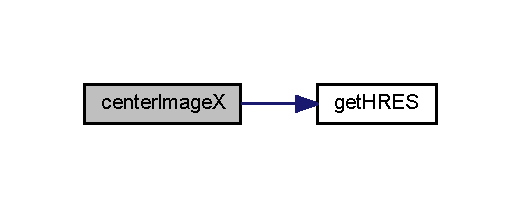
\includegraphics[width=250pt]{interface_8c_a2d06ffd4626bb0d6bb6b6bccb7feb3c3_cgraph}
\end{center}
\end{figure}


\hypertarget{interface_8c_a97f9bd0d20e1e9481357a22084763da7}{}\index{interface.\+c@{interface.\+c}!clean\+Cursor@{clean\+Cursor}}
\index{clean\+Cursor@{clean\+Cursor}!interface.\+c@{interface.\+c}}
\subsubsection[{clean\+Cursor}]{\setlength{\rightskip}{0pt plus 5cm}void clean\+Cursor (
\begin{DoxyParamCaption}
\item[{{\bf mouse\+\_\+state}}]{current\+\_\+mouse\+\_\+state}
\end{DoxyParamCaption}
)}\label{interface_8c_a97f9bd0d20e1e9481357a22084763da7}
Erases the cursor from the screen according to \hyperlink{structmouse__state}{mouse\+\_\+state} coordinates 
\begin{DoxyParams}{Parameters}
{\em current\+\_\+mouse\+\_\+state} & \\
\hline
\end{DoxyParams}


Definition at line 42 of file interface.\+c.



Here is the call graph for this function\+:\nopagebreak
\begin{figure}[H]
\begin{center}
\leavevmode
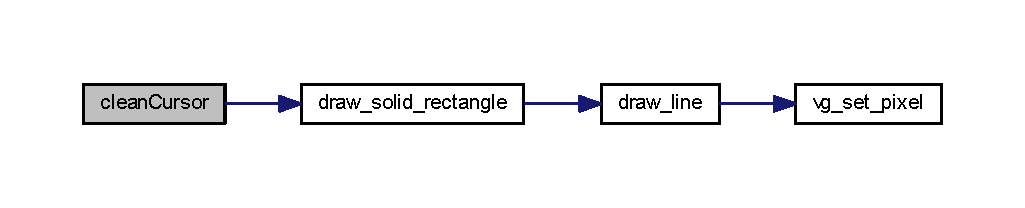
\includegraphics[width=350pt]{interface_8c_a97f9bd0d20e1e9481357a22084763da7_cgraph}
\end{center}
\end{figure}


\hypertarget{interface_8c_a79fd6c1e1239d1f44ed8cc6a3f9bbbe1}{}\index{interface.\+c@{interface.\+c}!clean\+Screen@{clean\+Screen}}
\index{clean\+Screen@{clean\+Screen}!interface.\+c@{interface.\+c}}
\subsubsection[{clean\+Screen}]{\setlength{\rightskip}{0pt plus 5cm}void clean\+Screen (
\begin{DoxyParamCaption}
{}
\end{DoxyParamCaption}
)}\label{interface_8c_a79fd6c1e1239d1f44ed8cc6a3f9bbbe1}
Cleans the screen 

Definition at line 59 of file interface.\+c.



Here is the call graph for this function\+:\nopagebreak
\begin{figure}[H]
\begin{center}
\leavevmode
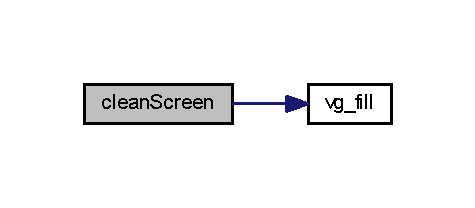
\includegraphics[width=228pt]{interface_8c_a79fd6c1e1239d1f44ed8cc6a3f9bbbe1_cgraph}
\end{center}
\end{figure}


\hypertarget{interface_8c_adab943f9f51fa4b94caccb44bb578ea0}{}\index{interface.\+c@{interface.\+c}!draw\+\_\+letter@{draw\+\_\+letter}}
\index{draw\+\_\+letter@{draw\+\_\+letter}!interface.\+c@{interface.\+c}}
\subsubsection[{draw\+\_\+letter}]{\setlength{\rightskip}{0pt plus 5cm}void draw\+\_\+letter (
\begin{DoxyParamCaption}
\item[{char}]{letter, }
\item[{int}]{x\+In, }
\item[{int}]{y\+In}
\end{DoxyParamCaption}
)}\label{interface_8c_adab943f9f51fa4b94caccb44bb578ea0}
Draws letters 

Definition at line 101 of file interface.\+c.



Here is the call graph for this function\+:\nopagebreak
\begin{figure}[H]
\begin{center}
\leavevmode
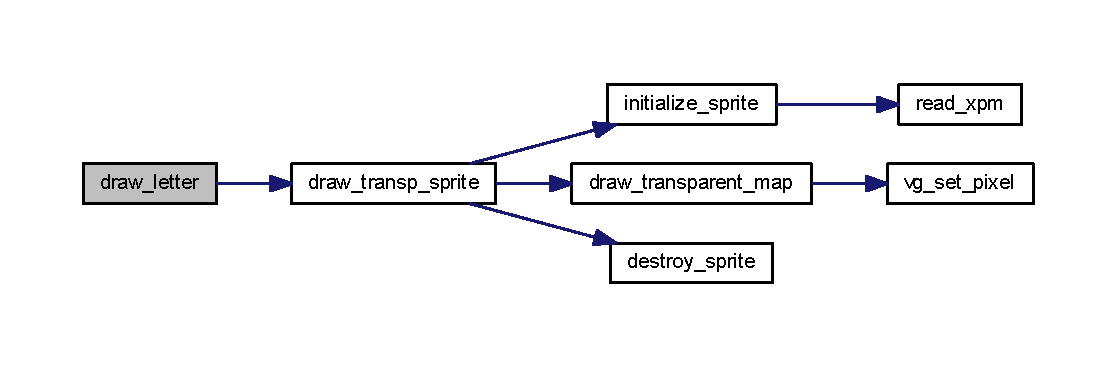
\includegraphics[width=350pt]{interface_8c_adab943f9f51fa4b94caccb44bb578ea0_cgraph}
\end{center}
\end{figure}


\hypertarget{interface_8c_a53105180167cdfba24a8c9f7ac6f0c2b}{}\index{interface.\+c@{interface.\+c}!draw\+\_\+string@{draw\+\_\+string}}
\index{draw\+\_\+string@{draw\+\_\+string}!interface.\+c@{interface.\+c}}
\subsubsection[{draw\+\_\+string}]{\setlength{\rightskip}{0pt plus 5cm}void draw\+\_\+string (
\begin{DoxyParamCaption}
\item[{char $\ast$}]{string, }
\item[{int}]{position\+X, }
\item[{int}]{position\+Y}
\end{DoxyParamCaption}
)}\label{interface_8c_a53105180167cdfba24a8c9f7ac6f0c2b}
Receives a string and draws it starting from position\+X and position\+Y coordinates 
\begin{DoxyParams}{Parameters}
{\em string} & \\
\hline
{\em position\+X} & \\
\hline
{\em position\+Y} & \\
\hline
\end{DoxyParams}


Definition at line 230 of file interface.\+c.



Here is the call graph for this function\+:\nopagebreak
\begin{figure}[H]
\begin{center}
\leavevmode
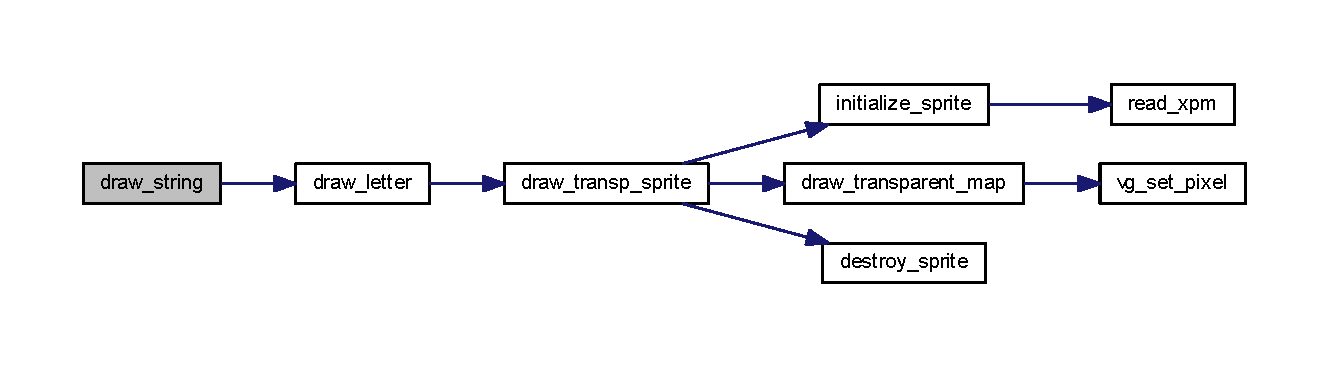
\includegraphics[width=350pt]{interface_8c_a53105180167cdfba24a8c9f7ac6f0c2b_cgraph}
\end{center}
\end{figure}


\hypertarget{interface_8c_acbd5457c126570af763ea24dc41da830}{}\index{interface.\+c@{interface.\+c}!draw\+Background@{draw\+Background}}
\index{draw\+Background@{draw\+Background}!interface.\+c@{interface.\+c}}
\subsubsection[{draw\+Background}]{\setlength{\rightskip}{0pt plus 5cm}void draw\+Background (
\begin{DoxyParamCaption}
{}
\end{DoxyParamCaption}
)}\label{interface_8c_acbd5457c126570af763ea24dc41da830}
Draws the background 

Definition at line 37 of file interface.\+c.



Here is the call graph for this function\+:\nopagebreak
\begin{figure}[H]
\begin{center}
\leavevmode
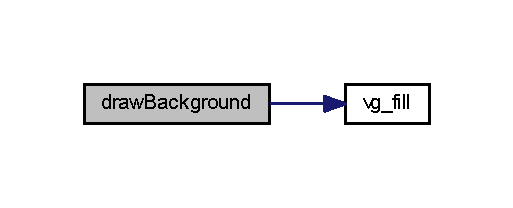
\includegraphics[width=246pt]{interface_8c_acbd5457c126570af763ea24dc41da830_cgraph}
\end{center}
\end{figure}


\hypertarget{interface_8c_a53b9d58cdef13b9d6394064ff6f9174e}{}\index{interface.\+c@{interface.\+c}!draw\+Clock@{draw\+Clock}}
\index{draw\+Clock@{draw\+Clock}!interface.\+c@{interface.\+c}}
\subsubsection[{draw\+Clock}]{\setlength{\rightskip}{0pt plus 5cm}void draw\+Clock (
\begin{DoxyParamCaption}
\item[{{\bf rtc\+\_\+state}}]{current\+\_\+rtc\+\_\+state}
\end{DoxyParamCaption}
)}\label{interface_8c_a53b9d58cdef13b9d6394064ff6f9174e}
Draws Clock according to its current state 
\begin{DoxyParams}{Parameters}
{\em current\+\_\+rtc\+\_\+state} & \\
\hline
\end{DoxyParams}


Definition at line 266 of file interface.\+c.



Here is the call graph for this function\+:\nopagebreak
\begin{figure}[H]
\begin{center}
\leavevmode
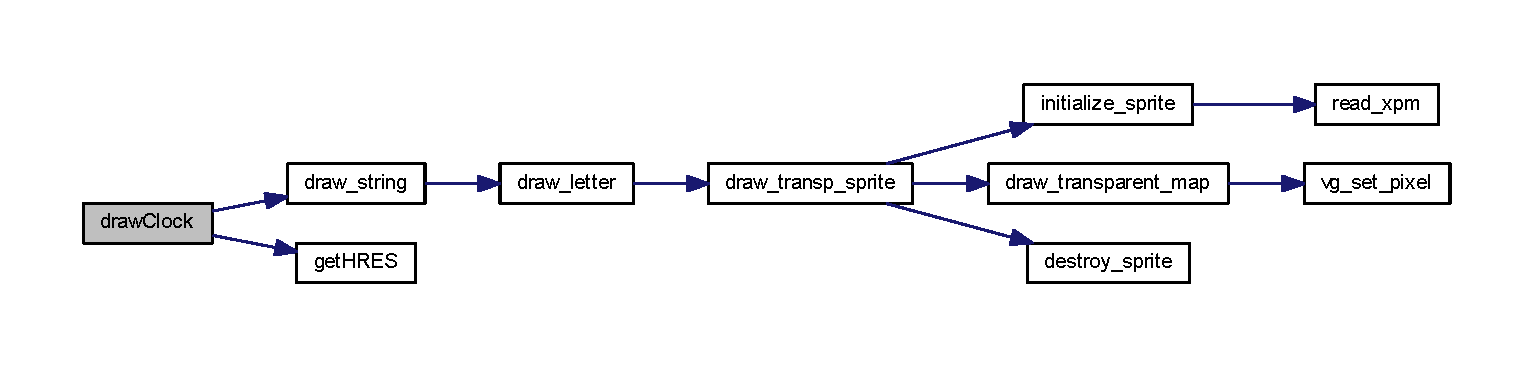
\includegraphics[width=350pt]{interface_8c_a53b9d58cdef13b9d6394064ff6f9174e_cgraph}
\end{center}
\end{figure}


\hypertarget{interface_8c_ad3f8d3bb7fc973176fd1a4d2de147beb}{}\index{interface.\+c@{interface.\+c}!draw\+Cursor@{draw\+Cursor}}
\index{draw\+Cursor@{draw\+Cursor}!interface.\+c@{interface.\+c}}
\subsubsection[{draw\+Cursor}]{\setlength{\rightskip}{0pt plus 5cm}void draw\+Cursor (
\begin{DoxyParamCaption}
\item[{{\bf mouse\+\_\+state}}]{current\+\_\+mouse\+\_\+state}
\end{DoxyParamCaption}
)}\label{interface_8c_ad3f8d3bb7fc973176fd1a4d2de147beb}
Draws the cursor on the screen according to \hyperlink{structmouse__state}{mouse\+\_\+state} coordinates 
\begin{DoxyParams}{Parameters}
{\em current\+\_\+mouse\+\_\+state} & \\
\hline
\end{DoxyParams}


Definition at line 29 of file interface.\+c.



Here is the call graph for this function\+:\nopagebreak
\begin{figure}[H]
\begin{center}
\leavevmode
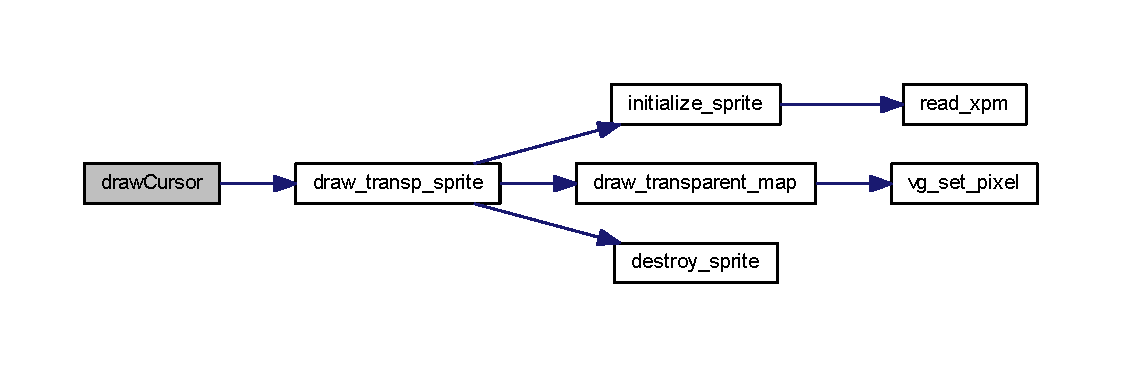
\includegraphics[width=350pt]{interface_8c_ad3f8d3bb7fc973176fd1a4d2de147beb_cgraph}
\end{center}
\end{figure}


\hypertarget{interface_8c_a26626ea6081aecf9fbce1d504567749d}{}\index{interface.\+c@{interface.\+c}!draw\+File@{draw\+File}}
\index{draw\+File@{draw\+File}!interface.\+c@{interface.\+c}}
\subsubsection[{draw\+File}]{\setlength{\rightskip}{0pt plus 5cm}void draw\+File (
\begin{DoxyParamCaption}
\item[{char $\ast$}]{file\+Path}
\end{DoxyParamCaption}
)}\label{interface_8c_a26626ea6081aecf9fbce1d504567749d}
Draws file to the screen (not fully working) 

Definition at line 214 of file interface.\+c.



Here is the call graph for this function\+:\nopagebreak
\begin{figure}[H]
\begin{center}
\leavevmode
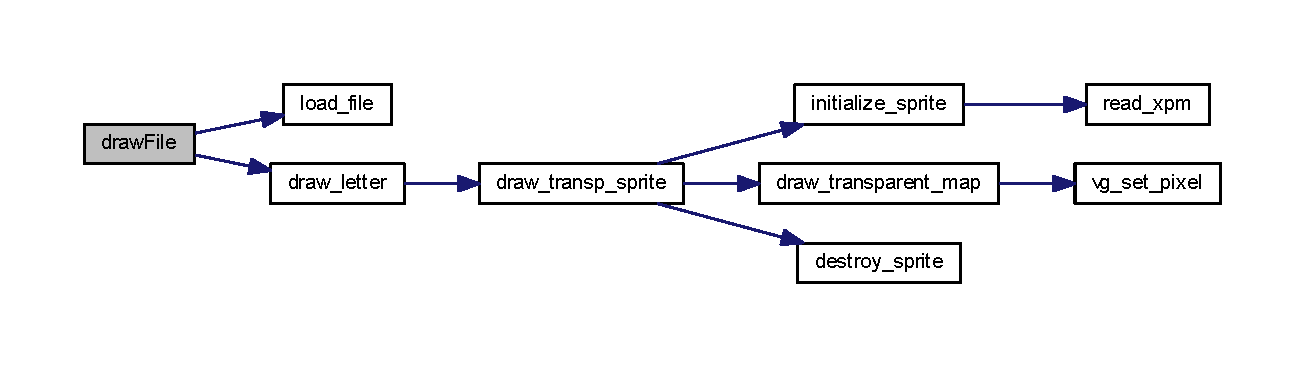
\includegraphics[width=350pt]{interface_8c_a26626ea6081aecf9fbce1d504567749d_cgraph}
\end{center}
\end{figure}


\hypertarget{interface_8c_a05505f25859a670bb3d5eb8df6fd5f23}{}\index{interface.\+c@{interface.\+c}!draw\+Folders@{draw\+Folders}}
\index{draw\+Folders@{draw\+Folders}!interface.\+c@{interface.\+c}}
\subsubsection[{draw\+Folders}]{\setlength{\rightskip}{0pt plus 5cm}void draw\+Folders (
\begin{DoxyParamCaption}
{}
\end{DoxyParamCaption}
)}\label{interface_8c_a05505f25859a670bb3d5eb8df6fd5f23}
Draws the folders and files on the screen 

Definition at line 314 of file interface.\+c.



Here is the call graph for this function\+:\nopagebreak
\begin{figure}[H]
\begin{center}
\leavevmode
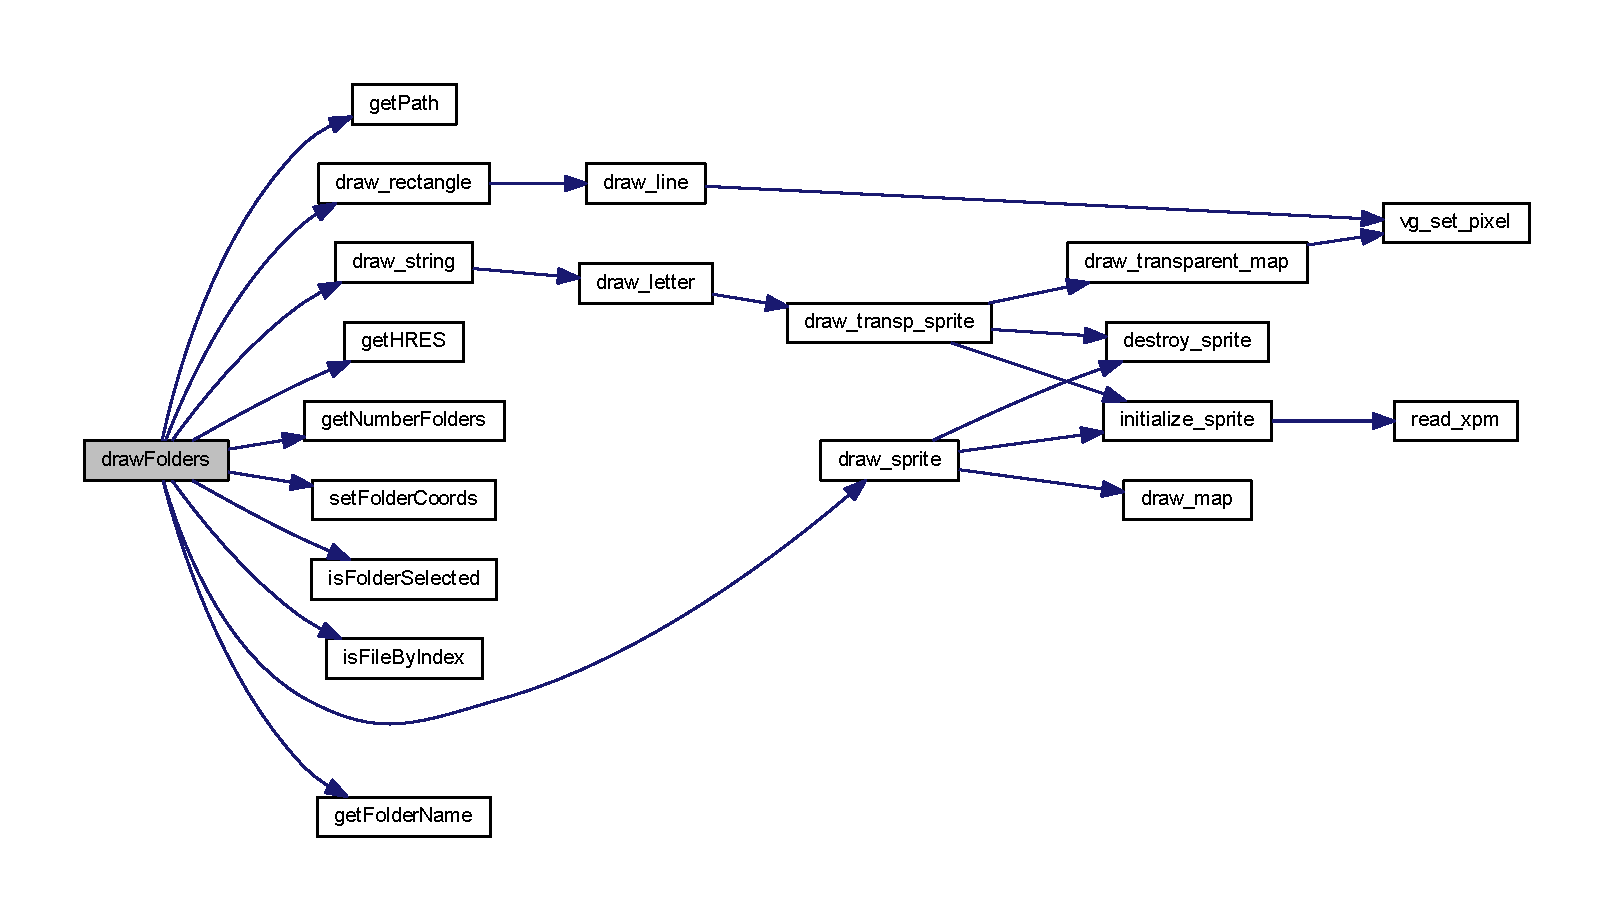
\includegraphics[width=350pt]{interface_8c_a05505f25859a670bb3d5eb8df6fd5f23_cgraph}
\end{center}
\end{figure}


\hypertarget{interface_8c_a374a1af3e9988185e4bcb999ec29ccd7}{}\index{interface.\+c@{interface.\+c}!draw\+Input\+Box@{draw\+Input\+Box}}
\index{draw\+Input\+Box@{draw\+Input\+Box}!interface.\+c@{interface.\+c}}
\subsubsection[{draw\+Input\+Box}]{\setlength{\rightskip}{0pt plus 5cm}void draw\+Input\+Box (
\begin{DoxyParamCaption}
\item[{char $\ast$}]{title, }
\item[{char $\ast$}]{message}
\end{DoxyParamCaption}
)}\label{interface_8c_a374a1af3e9988185e4bcb999ec29ccd7}
Draws input box for rename purposes 
\begin{DoxyParams}{Parameters}
{\em title} & \\
\hline
{\em message} & \\
\hline
\end{DoxyParams}


Definition at line 64 of file interface.\+c.



Here is the call graph for this function\+:\nopagebreak
\begin{figure}[H]
\begin{center}
\leavevmode
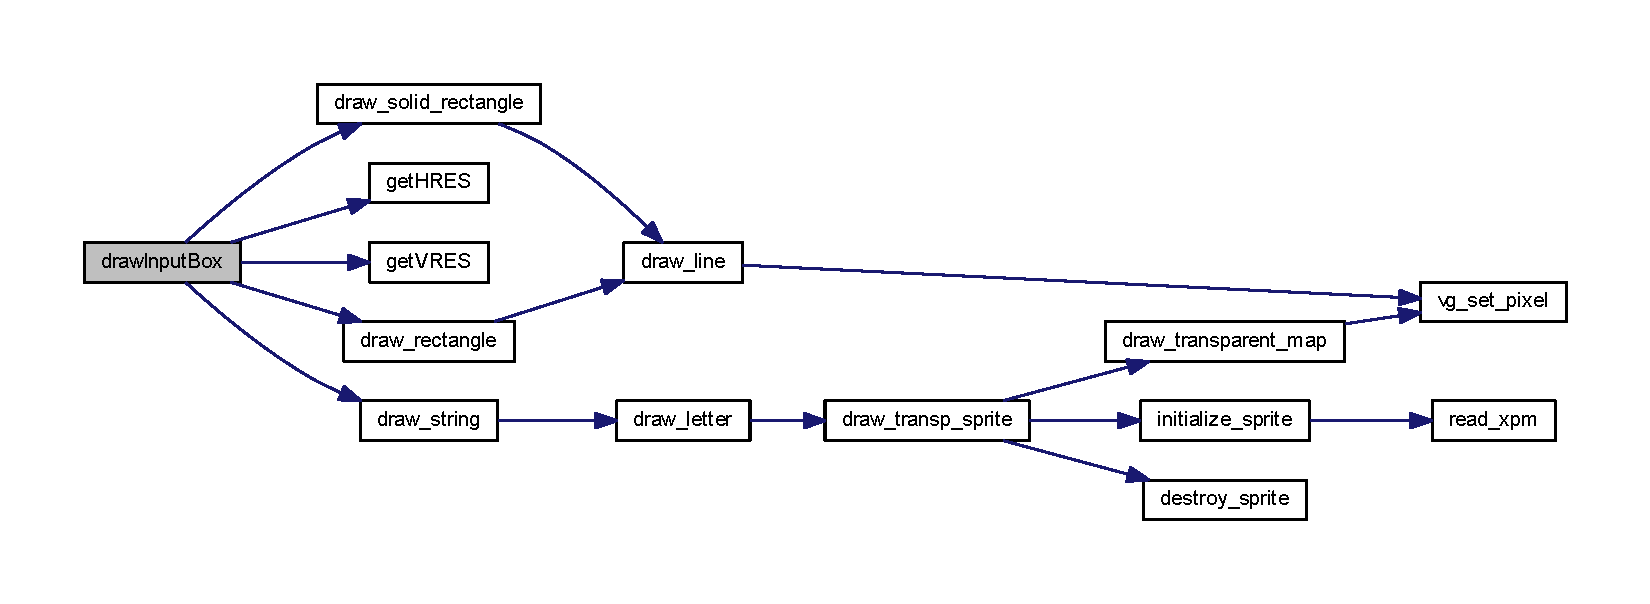
\includegraphics[width=350pt]{interface_8c_a374a1af3e9988185e4bcb999ec29ccd7_cgraph}
\end{center}
\end{figure}


\hypertarget{interface_8c_a06326bc3ce2fdfe90cb6eb3172159fd0}{}\index{interface.\+c@{interface.\+c}!draw\+Main\+Menu@{draw\+Main\+Menu}}
\index{draw\+Main\+Menu@{draw\+Main\+Menu}!interface.\+c@{interface.\+c}}
\subsubsection[{draw\+Main\+Menu}]{\setlength{\rightskip}{0pt plus 5cm}void draw\+Main\+Menu (
\begin{DoxyParamCaption}
{}
\end{DoxyParamCaption}
)}\label{interface_8c_a06326bc3ce2fdfe90cb6eb3172159fd0}
Draws main menu 

Definition at line 46 of file interface.\+c.



Here is the call graph for this function\+:\nopagebreak
\begin{figure}[H]
\begin{center}
\leavevmode
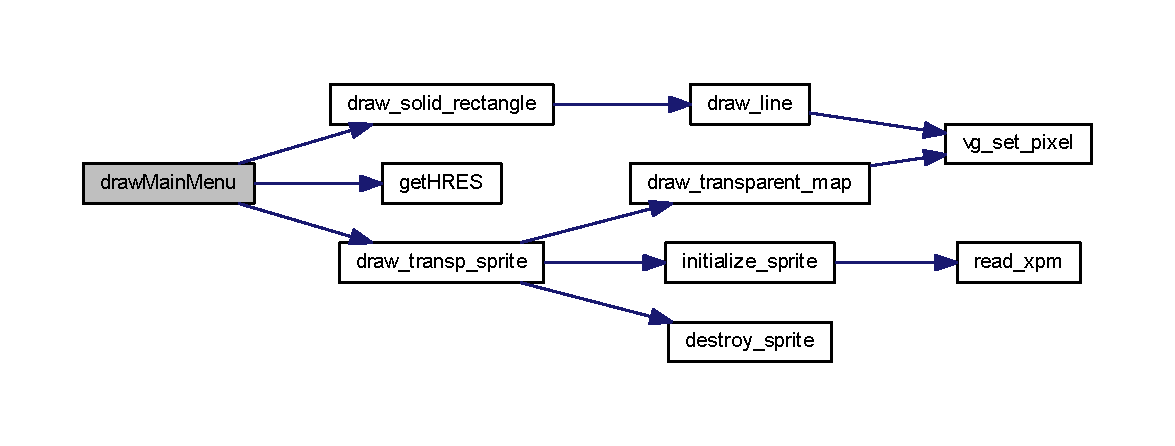
\includegraphics[width=350pt]{interface_8c_a06326bc3ce2fdfe90cb6eb3172159fd0_cgraph}
\end{center}
\end{figure}


\hypertarget{interface_8c_a04b43cf8b4fbf16e17cea07e7daf8bf9}{}\index{interface.\+c@{interface.\+c}!draw\+Output\+Box@{draw\+Output\+Box}}
\index{draw\+Output\+Box@{draw\+Output\+Box}!interface.\+c@{interface.\+c}}
\subsubsection[{draw\+Output\+Box}]{\setlength{\rightskip}{0pt plus 5cm}void draw\+Output\+Box (
\begin{DoxyParamCaption}
\item[{char $\ast$}]{title, }
\item[{char $\ast$}]{message}
\end{DoxyParamCaption}
)}\label{interface_8c_a04b43cf8b4fbf16e17cea07e7daf8bf9}
Draws a pop-\/up box with title and message 
\begin{DoxyParams}{Parameters}
{\em title} & \\
\hline
{\em message} & \\
\hline
\end{DoxyParams}


Definition at line 84 of file interface.\+c.



Here is the call graph for this function\+:\nopagebreak
\begin{figure}[H]
\begin{center}
\leavevmode
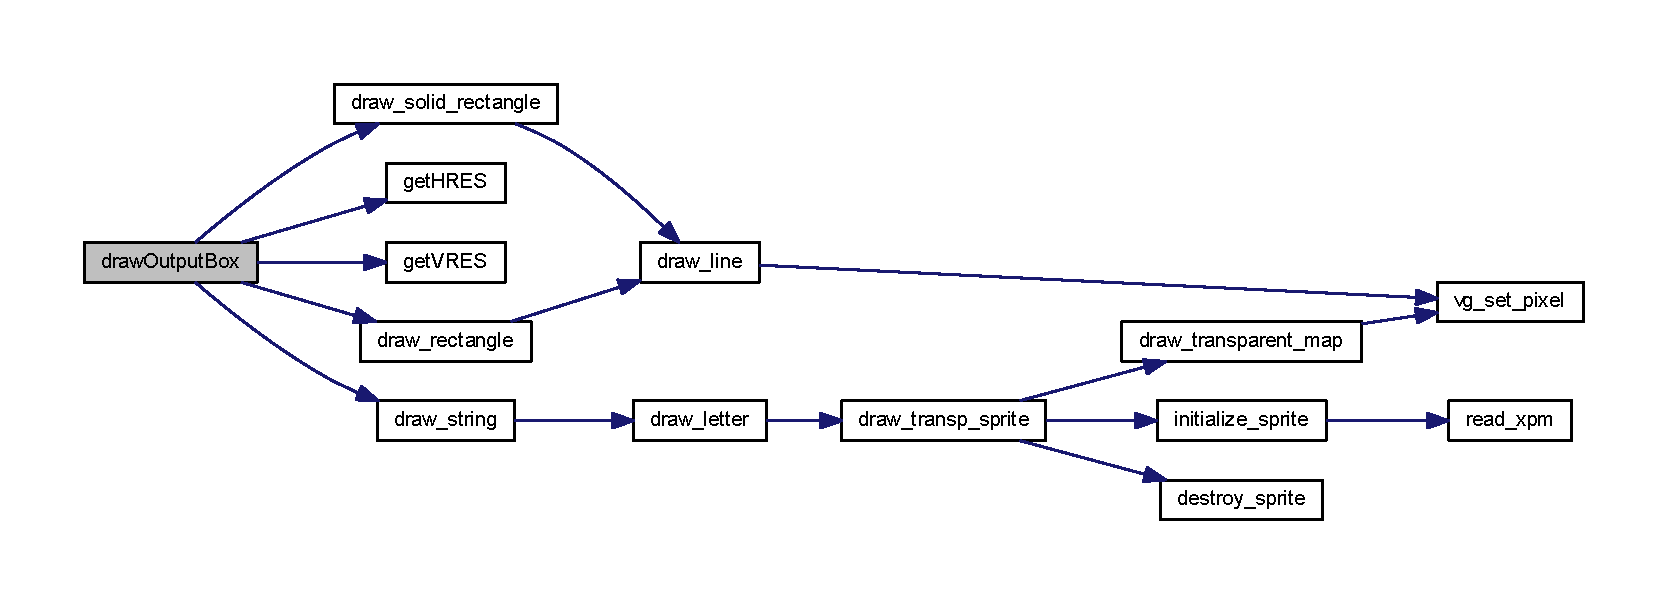
\includegraphics[width=350pt]{interface_8c_a04b43cf8b4fbf16e17cea07e7daf8bf9_cgraph}
\end{center}
\end{figure}


\hypertarget{interface_8c_a7191ba49f3495cfb9304adc2a6661d7e}{}\index{interface.\+c@{interface.\+c}!draw\+Right\+Click\+Menu@{draw\+Right\+Click\+Menu}}
\index{draw\+Right\+Click\+Menu@{draw\+Right\+Click\+Menu}!interface.\+c@{interface.\+c}}
\subsubsection[{draw\+Right\+Click\+Menu}]{\setlength{\rightskip}{0pt plus 5cm}void draw\+Right\+Click\+Menu (
\begin{DoxyParamCaption}
\item[{{\bf mouse\+\_\+state}}]{current\+\_\+mouse\+\_\+state}
\end{DoxyParamCaption}
)}\label{interface_8c_a7191ba49f3495cfb9304adc2a6661d7e}
Draws right click menu according to \hyperlink{structmouse__state}{mouse\+\_\+state} coordinates 
\begin{DoxyParams}{Parameters}
{\em current\+\_\+mouse\+\_\+state} & \\
\hline
\end{DoxyParams}


Definition at line 247 of file interface.\+c.



Here is the call graph for this function\+:\nopagebreak
\begin{figure}[H]
\begin{center}
\leavevmode
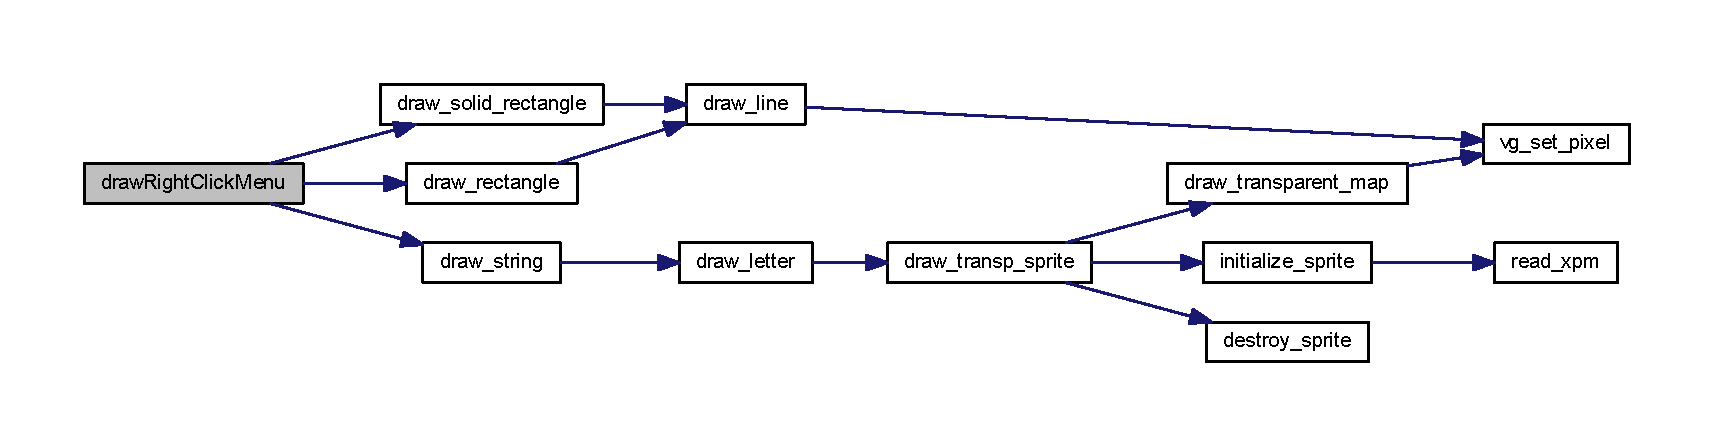
\includegraphics[width=350pt]{interface_8c_a7191ba49f3495cfb9304adc2a6661d7e_cgraph}
\end{center}
\end{figure}


\hypertarget{interface_8c_a1416e34c293ab47d9ba58c0c3326605a}{}\index{interface.\+c@{interface.\+c}!load\+\_\+file@{load\+\_\+file}}
\index{load\+\_\+file@{load\+\_\+file}!interface.\+c@{interface.\+c}}
\subsubsection[{load\+\_\+file}]{\setlength{\rightskip}{0pt plus 5cm}char$\ast$ load\+\_\+file (
\begin{DoxyParamCaption}
\item[{char $\ast$}]{file\+Path}
\end{DoxyParamCaption}
)}\label{interface_8c_a1416e34c293ab47d9ba58c0c3326605a}


Definition at line 182 of file interface.\+c.

\hypertarget{interface_8c_aaee65a42f436525f7b9887fbe4f3663d}{}\index{interface.\+c@{interface.\+c}!main\+Draw@{main\+Draw}}
\index{main\+Draw@{main\+Draw}!interface.\+c@{interface.\+c}}
\subsubsection[{main\+Draw}]{\setlength{\rightskip}{0pt plus 5cm}void main\+Draw (
\begin{DoxyParamCaption}
{}
\end{DoxyParamCaption}
)}\label{interface_8c_aaee65a42f436525f7b9887fbe4f3663d}
Draws the initial interface (Penguin, logo and developers) 

Definition at line 7 of file interface.\+c.



Here is the call graph for this function\+:\nopagebreak
\begin{figure}[H]
\begin{center}
\leavevmode
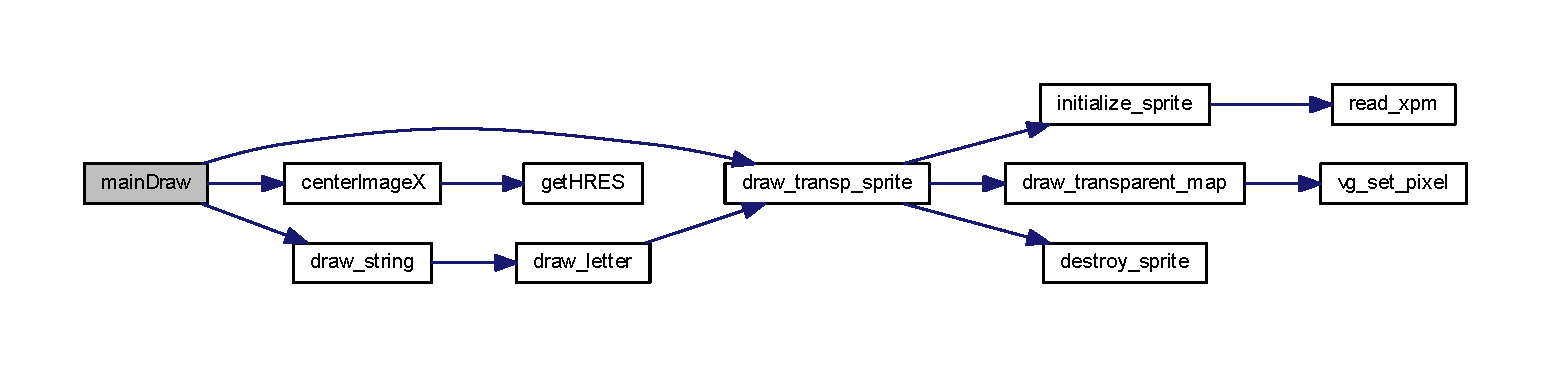
\includegraphics[width=350pt]{interface_8c_aaee65a42f436525f7b9887fbe4f3663d_cgraph}
\end{center}
\end{figure}



\hypertarget{interface_8h}{}\section{interface.\+h File Reference}
\label{interface_8h}\index{interface.\+h@{interface.\+h}}
{\ttfamily \#include \char`\"{}pixmap.\+c\char`\"{}}\\*
{\ttfamily \#include \char`\"{}video\+\_\+gr.\+h\char`\"{}}\\*
{\ttfamily \#include \char`\"{}mouse.\+h\char`\"{}}\\*
{\ttfamily \#include \char`\"{}logic.\+h\char`\"{}}\\*
{\ttfamily \#include \char`\"{}rtc.\+h\char`\"{}}\\*
\subsection*{Functions}
\begin{DoxyCompactItemize}
\item 
int \hyperlink{interface_8h_a2d06ffd4626bb0d6bb6b6bccb7feb3c3}{center\+Image\+X} (int image\+Width)
\item 
void \hyperlink{interface_8h_aaee65a42f436525f7b9887fbe4f3663d}{main\+Draw} ()
\item 
void \hyperlink{interface_8h_ad3f8d3bb7fc973176fd1a4d2de147beb}{draw\+Cursor} (\hyperlink{structmouse__state}{mouse\+\_\+state} \hyperlink{state_8h_a39d9a371f9aef2042923a96e2f855d5e}{current\+\_\+mouse\+\_\+state})
\item 
void \hyperlink{interface_8h_acbd5457c126570af763ea24dc41da830}{draw\+Background} ()
\item 
void \hyperlink{interface_8h_a97f9bd0d20e1e9481357a22084763da7}{clean\+Cursor} (\hyperlink{structmouse__state}{mouse\+\_\+state} \hyperlink{state_8h_a39d9a371f9aef2042923a96e2f855d5e}{current\+\_\+mouse\+\_\+state})
\item 
void \hyperlink{interface_8h_a06326bc3ce2fdfe90cb6eb3172159fd0}{draw\+Main\+Menu} ()
\item 
void \hyperlink{interface_8h_a79fd6c1e1239d1f44ed8cc6a3f9bbbe1}{clean\+Screen} ()
\item 
void \hyperlink{interface_8h_a6f3710a0deef4dec8c40e1387f00b2cf}{draw\+Input\+Box} (char $\ast$title, char $\ast$message)
\item 
void \hyperlink{interface_8h_a04b43cf8b4fbf16e17cea07e7daf8bf9}{draw\+Output\+Box} (char $\ast$title, char $\ast$message)
\item 
void \hyperlink{interface_8h_adab943f9f51fa4b94caccb44bb578ea0}{draw\+\_\+letter} (char letter, int x\+In, int y\+In)
\item 
void \hyperlink{interface_8h_a26626ea6081aecf9fbce1d504567749d}{draw\+File} (char $\ast$file\+Path)
\item 
void \hyperlink{interface_8h_a53105180167cdfba24a8c9f7ac6f0c2b}{draw\+\_\+string} (char $\ast$string, int position\+X, int position\+Y)
\item 
void \hyperlink{interface_8h_a7191ba49f3495cfb9304adc2a6661d7e}{draw\+Right\+Click\+Menu} (\hyperlink{structmouse__state}{mouse\+\_\+state} \hyperlink{state_8h_a39d9a371f9aef2042923a96e2f855d5e}{current\+\_\+mouse\+\_\+state})
\item 
void \hyperlink{interface_8h_a53b9d58cdef13b9d6394064ff6f9174e}{draw\+Clock} (\hyperlink{structrtc__state}{rtc\+\_\+state} \hyperlink{state_8h_aab5669abb2a76b898c30b667998b6f1e}{current\+\_\+rtc\+\_\+state})
\item 
void \hyperlink{interface_8h_a05505f25859a670bb3d5eb8df6fd5f23}{draw\+Folders} ()
\end{DoxyCompactItemize}


\subsection{Function Documentation}
\hypertarget{interface_8h_a2d06ffd4626bb0d6bb6b6bccb7feb3c3}{}\index{interface.\+h@{interface.\+h}!center\+Image\+X@{center\+Image\+X}}
\index{center\+Image\+X@{center\+Image\+X}!interface.\+h@{interface.\+h}}
\subsubsection[{center\+Image\+X}]{\setlength{\rightskip}{0pt plus 5cm}int center\+Image\+X (
\begin{DoxyParamCaption}
\item[{int}]{image\+Width}
\end{DoxyParamCaption}
)}\label{interface_8h_a2d06ffd4626bb0d6bb6b6bccb7feb3c3}
Centers an image on the screen


\begin{DoxyParams}{Parameters}
{\em image\+Width} & \\
\hline
\end{DoxyParams}
\begin{DoxyReturn}{Returns}

\end{DoxyReturn}


Definition at line 3 of file interface.\+c.



Here is the call graph for this function\+:\nopagebreak
\begin{figure}[H]
\begin{center}
\leavevmode
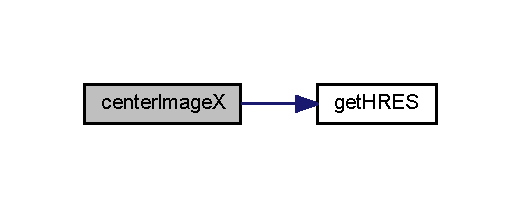
\includegraphics[width=250pt]{interface_8h_a2d06ffd4626bb0d6bb6b6bccb7feb3c3_cgraph}
\end{center}
\end{figure}


\hypertarget{interface_8h_a97f9bd0d20e1e9481357a22084763da7}{}\index{interface.\+h@{interface.\+h}!clean\+Cursor@{clean\+Cursor}}
\index{clean\+Cursor@{clean\+Cursor}!interface.\+h@{interface.\+h}}
\subsubsection[{clean\+Cursor}]{\setlength{\rightskip}{0pt plus 5cm}void clean\+Cursor (
\begin{DoxyParamCaption}
\item[{{\bf mouse\+\_\+state}}]{current\+\_\+mouse\+\_\+state}
\end{DoxyParamCaption}
)}\label{interface_8h_a97f9bd0d20e1e9481357a22084763da7}
Erases the cursor from the screen according to \hyperlink{structmouse__state}{mouse\+\_\+state} coordinates 
\begin{DoxyParams}{Parameters}
{\em current\+\_\+mouse\+\_\+state} & \\
\hline
\end{DoxyParams}


Definition at line 42 of file interface.\+c.



Here is the call graph for this function\+:\nopagebreak
\begin{figure}[H]
\begin{center}
\leavevmode
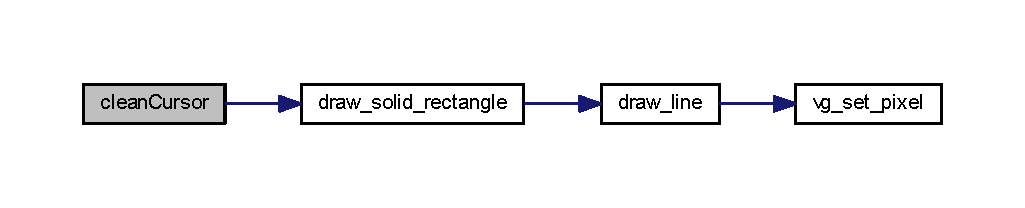
\includegraphics[width=350pt]{interface_8h_a97f9bd0d20e1e9481357a22084763da7_cgraph}
\end{center}
\end{figure}


\hypertarget{interface_8h_a79fd6c1e1239d1f44ed8cc6a3f9bbbe1}{}\index{interface.\+h@{interface.\+h}!clean\+Screen@{clean\+Screen}}
\index{clean\+Screen@{clean\+Screen}!interface.\+h@{interface.\+h}}
\subsubsection[{clean\+Screen}]{\setlength{\rightskip}{0pt plus 5cm}void clean\+Screen (
\begin{DoxyParamCaption}
{}
\end{DoxyParamCaption}
)}\label{interface_8h_a79fd6c1e1239d1f44ed8cc6a3f9bbbe1}
Cleans the screen 

Definition at line 59 of file interface.\+c.



Here is the call graph for this function\+:\nopagebreak
\begin{figure}[H]
\begin{center}
\leavevmode
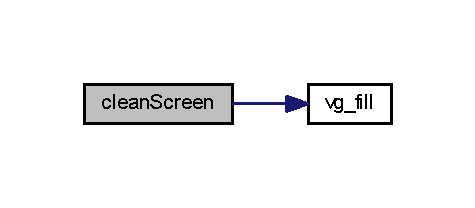
\includegraphics[width=228pt]{interface_8h_a79fd6c1e1239d1f44ed8cc6a3f9bbbe1_cgraph}
\end{center}
\end{figure}


\hypertarget{interface_8h_adab943f9f51fa4b94caccb44bb578ea0}{}\index{interface.\+h@{interface.\+h}!draw\+\_\+letter@{draw\+\_\+letter}}
\index{draw\+\_\+letter@{draw\+\_\+letter}!interface.\+h@{interface.\+h}}
\subsubsection[{draw\+\_\+letter}]{\setlength{\rightskip}{0pt plus 5cm}void draw\+\_\+letter (
\begin{DoxyParamCaption}
\item[{char}]{letter, }
\item[{int}]{x\+In, }
\item[{int}]{y\+In}
\end{DoxyParamCaption}
)}\label{interface_8h_adab943f9f51fa4b94caccb44bb578ea0}
Draws letters 

Definition at line 101 of file interface.\+c.



Here is the call graph for this function\+:\nopagebreak
\begin{figure}[H]
\begin{center}
\leavevmode
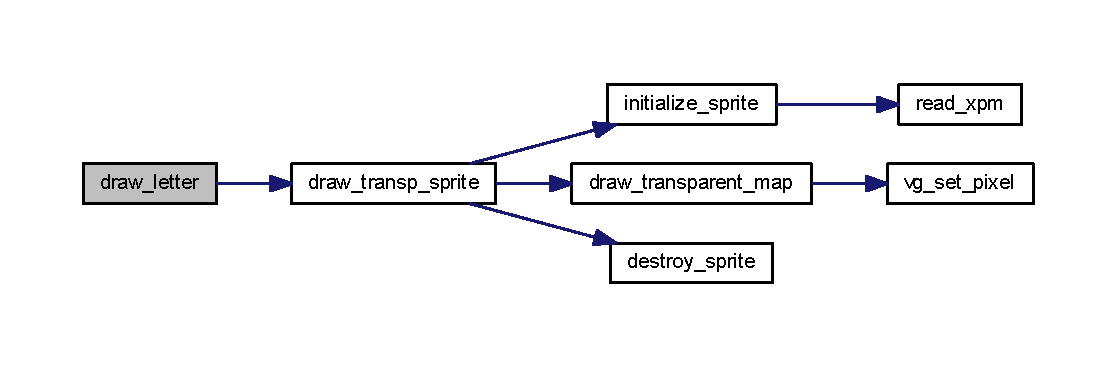
\includegraphics[width=350pt]{interface_8h_adab943f9f51fa4b94caccb44bb578ea0_cgraph}
\end{center}
\end{figure}


\hypertarget{interface_8h_a53105180167cdfba24a8c9f7ac6f0c2b}{}\index{interface.\+h@{interface.\+h}!draw\+\_\+string@{draw\+\_\+string}}
\index{draw\+\_\+string@{draw\+\_\+string}!interface.\+h@{interface.\+h}}
\subsubsection[{draw\+\_\+string}]{\setlength{\rightskip}{0pt plus 5cm}void draw\+\_\+string (
\begin{DoxyParamCaption}
\item[{char $\ast$}]{string, }
\item[{int}]{position\+X, }
\item[{int}]{position\+Y}
\end{DoxyParamCaption}
)}\label{interface_8h_a53105180167cdfba24a8c9f7ac6f0c2b}
Receives a string and draws it starting from position\+X and position\+Y coordinates 
\begin{DoxyParams}{Parameters}
{\em string} & \\
\hline
{\em position\+X} & \\
\hline
{\em position\+Y} & \\
\hline
\end{DoxyParams}


Definition at line 230 of file interface.\+c.



Here is the call graph for this function\+:\nopagebreak
\begin{figure}[H]
\begin{center}
\leavevmode
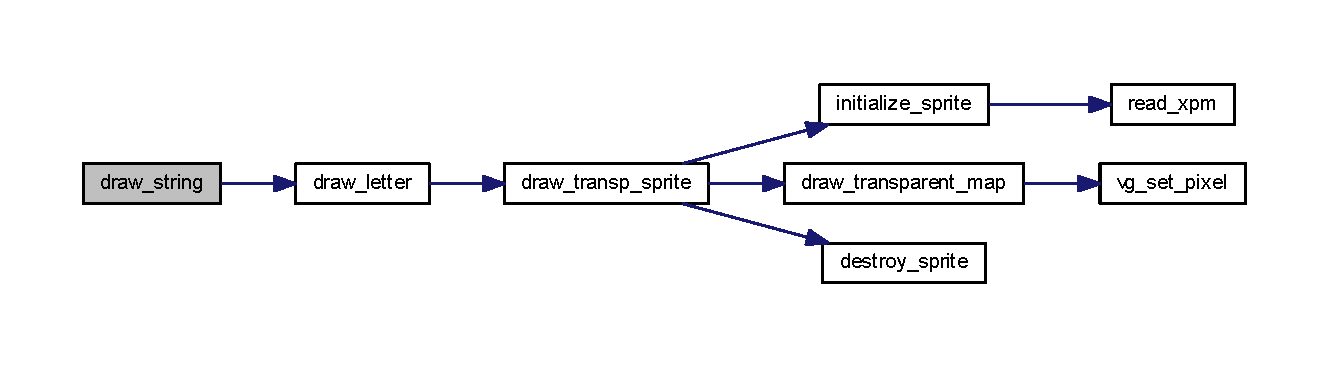
\includegraphics[width=350pt]{interface_8h_a53105180167cdfba24a8c9f7ac6f0c2b_cgraph}
\end{center}
\end{figure}


\hypertarget{interface_8h_acbd5457c126570af763ea24dc41da830}{}\index{interface.\+h@{interface.\+h}!draw\+Background@{draw\+Background}}
\index{draw\+Background@{draw\+Background}!interface.\+h@{interface.\+h}}
\subsubsection[{draw\+Background}]{\setlength{\rightskip}{0pt plus 5cm}void draw\+Background (
\begin{DoxyParamCaption}
{}
\end{DoxyParamCaption}
)}\label{interface_8h_acbd5457c126570af763ea24dc41da830}
Draws the background 

Definition at line 37 of file interface.\+c.



Here is the call graph for this function\+:\nopagebreak
\begin{figure}[H]
\begin{center}
\leavevmode
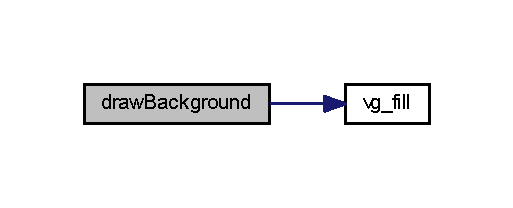
\includegraphics[width=246pt]{interface_8h_acbd5457c126570af763ea24dc41da830_cgraph}
\end{center}
\end{figure}


\hypertarget{interface_8h_a53b9d58cdef13b9d6394064ff6f9174e}{}\index{interface.\+h@{interface.\+h}!draw\+Clock@{draw\+Clock}}
\index{draw\+Clock@{draw\+Clock}!interface.\+h@{interface.\+h}}
\subsubsection[{draw\+Clock}]{\setlength{\rightskip}{0pt plus 5cm}void draw\+Clock (
\begin{DoxyParamCaption}
\item[{{\bf rtc\+\_\+state}}]{current\+\_\+rtc\+\_\+state}
\end{DoxyParamCaption}
)}\label{interface_8h_a53b9d58cdef13b9d6394064ff6f9174e}
Draws Clock according to its current state 
\begin{DoxyParams}{Parameters}
{\em current\+\_\+rtc\+\_\+state} & \\
\hline
\end{DoxyParams}


Definition at line 266 of file interface.\+c.



Here is the call graph for this function\+:\nopagebreak
\begin{figure}[H]
\begin{center}
\leavevmode
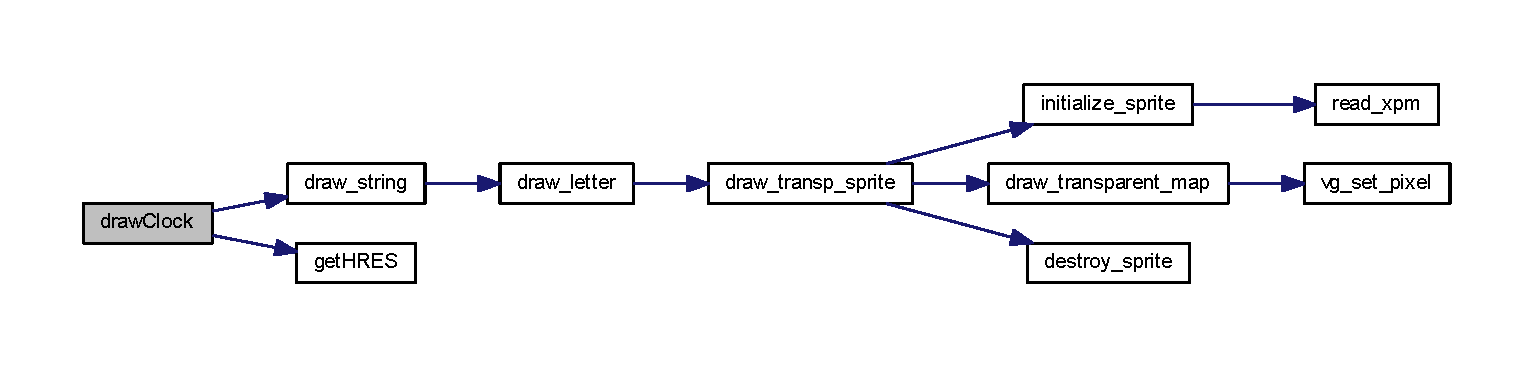
\includegraphics[width=350pt]{interface_8h_a53b9d58cdef13b9d6394064ff6f9174e_cgraph}
\end{center}
\end{figure}


\hypertarget{interface_8h_ad3f8d3bb7fc973176fd1a4d2de147beb}{}\index{interface.\+h@{interface.\+h}!draw\+Cursor@{draw\+Cursor}}
\index{draw\+Cursor@{draw\+Cursor}!interface.\+h@{interface.\+h}}
\subsubsection[{draw\+Cursor}]{\setlength{\rightskip}{0pt plus 5cm}void draw\+Cursor (
\begin{DoxyParamCaption}
\item[{{\bf mouse\+\_\+state}}]{current\+\_\+mouse\+\_\+state}
\end{DoxyParamCaption}
)}\label{interface_8h_ad3f8d3bb7fc973176fd1a4d2de147beb}
Draws the cursor on the screen according to \hyperlink{structmouse__state}{mouse\+\_\+state} coordinates 
\begin{DoxyParams}{Parameters}
{\em current\+\_\+mouse\+\_\+state} & \\
\hline
\end{DoxyParams}


Definition at line 29 of file interface.\+c.



Here is the call graph for this function\+:\nopagebreak
\begin{figure}[H]
\begin{center}
\leavevmode
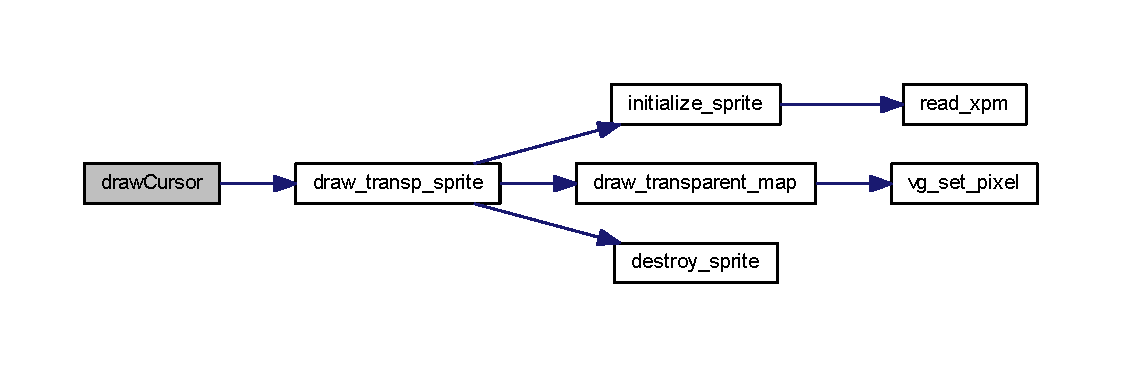
\includegraphics[width=350pt]{interface_8h_ad3f8d3bb7fc973176fd1a4d2de147beb_cgraph}
\end{center}
\end{figure}


\hypertarget{interface_8h_a26626ea6081aecf9fbce1d504567749d}{}\index{interface.\+h@{interface.\+h}!draw\+File@{draw\+File}}
\index{draw\+File@{draw\+File}!interface.\+h@{interface.\+h}}
\subsubsection[{draw\+File}]{\setlength{\rightskip}{0pt plus 5cm}void draw\+File (
\begin{DoxyParamCaption}
\item[{char $\ast$}]{file\+Path}
\end{DoxyParamCaption}
)}\label{interface_8h_a26626ea6081aecf9fbce1d504567749d}
Draws file to the screen (not fully working) 

Definition at line 214 of file interface.\+c.



Here is the call graph for this function\+:\nopagebreak
\begin{figure}[H]
\begin{center}
\leavevmode
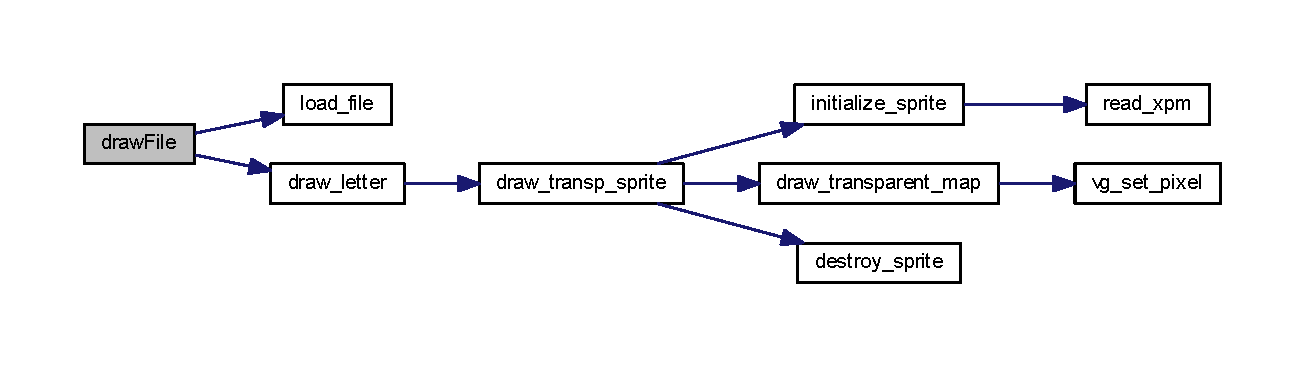
\includegraphics[width=350pt]{interface_8h_a26626ea6081aecf9fbce1d504567749d_cgraph}
\end{center}
\end{figure}


\hypertarget{interface_8h_a05505f25859a670bb3d5eb8df6fd5f23}{}\index{interface.\+h@{interface.\+h}!draw\+Folders@{draw\+Folders}}
\index{draw\+Folders@{draw\+Folders}!interface.\+h@{interface.\+h}}
\subsubsection[{draw\+Folders}]{\setlength{\rightskip}{0pt plus 5cm}void draw\+Folders (
\begin{DoxyParamCaption}
{}
\end{DoxyParamCaption}
)}\label{interface_8h_a05505f25859a670bb3d5eb8df6fd5f23}
Draws the folders and files on the screen 

Definition at line 314 of file interface.\+c.



Here is the call graph for this function\+:\nopagebreak
\begin{figure}[H]
\begin{center}
\leavevmode
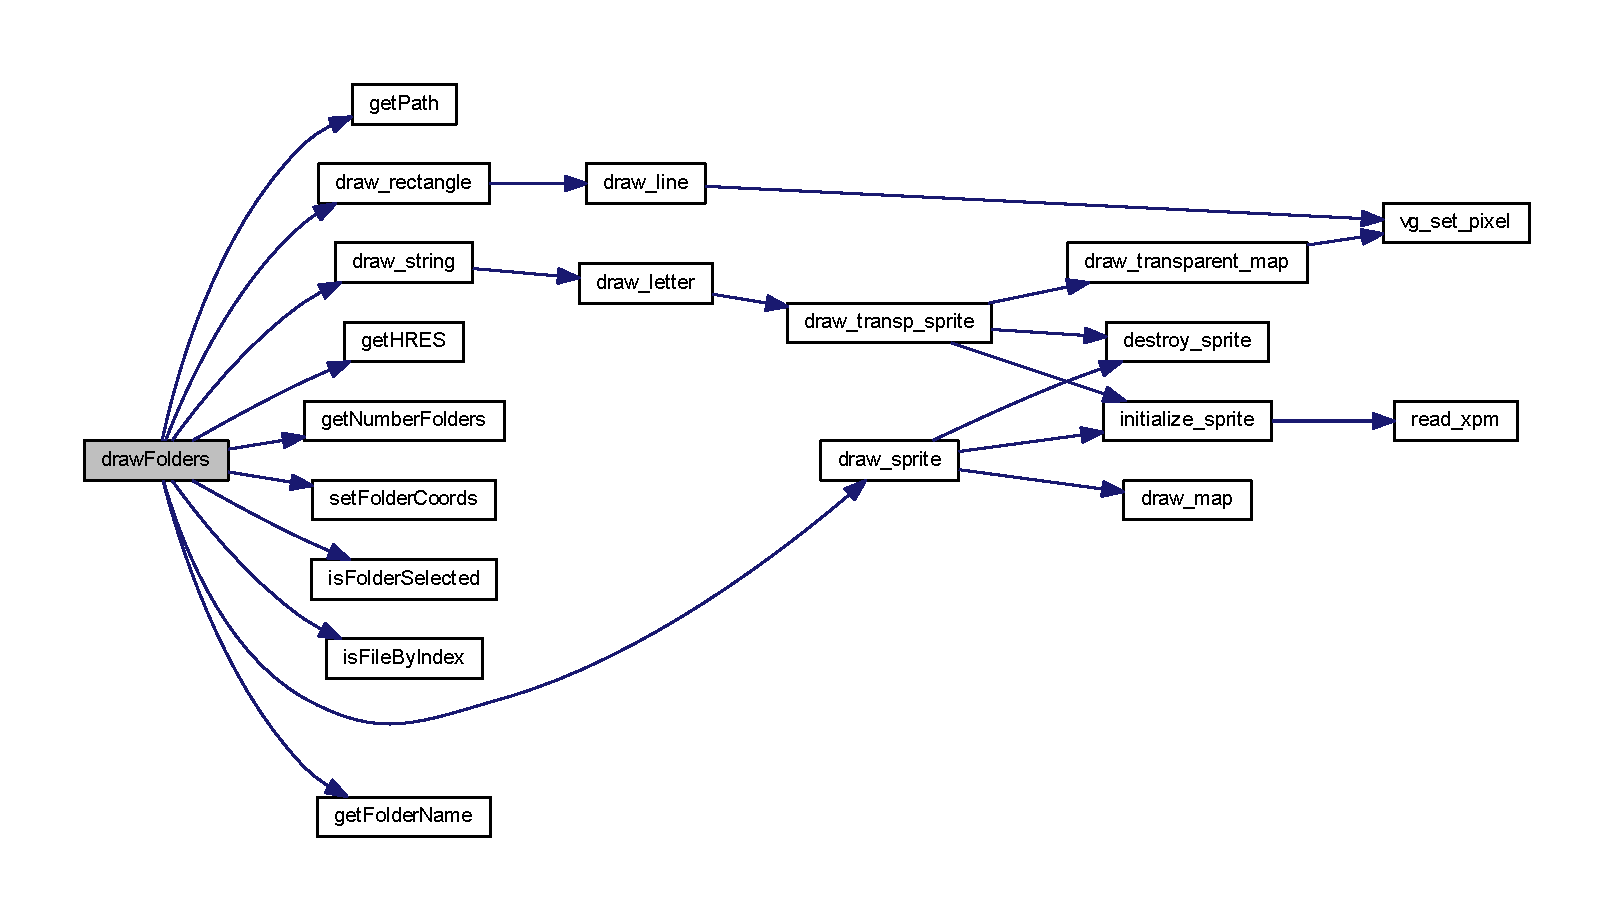
\includegraphics[width=350pt]{interface_8h_a05505f25859a670bb3d5eb8df6fd5f23_cgraph}
\end{center}
\end{figure}


\hypertarget{interface_8h_a6f3710a0deef4dec8c40e1387f00b2cf}{}\index{interface.\+h@{interface.\+h}!draw\+Input\+Box@{draw\+Input\+Box}}
\index{draw\+Input\+Box@{draw\+Input\+Box}!interface.\+h@{interface.\+h}}
\subsubsection[{draw\+Input\+Box}]{\setlength{\rightskip}{0pt plus 5cm}void draw\+Input\+Box (
\begin{DoxyParamCaption}
\item[{char $\ast$}]{title, }
\item[{char $\ast$}]{message}
\end{DoxyParamCaption}
)}\label{interface_8h_a6f3710a0deef4dec8c40e1387f00b2cf}
Draws input box for rename purposes 
\begin{DoxyParams}{Parameters}
{\em title} & \\
\hline
{\em message} & \\
\hline
\end{DoxyParams}


Definition at line 64 of file interface.\+c.



Here is the call graph for this function\+:\nopagebreak
\begin{figure}[H]
\begin{center}
\leavevmode
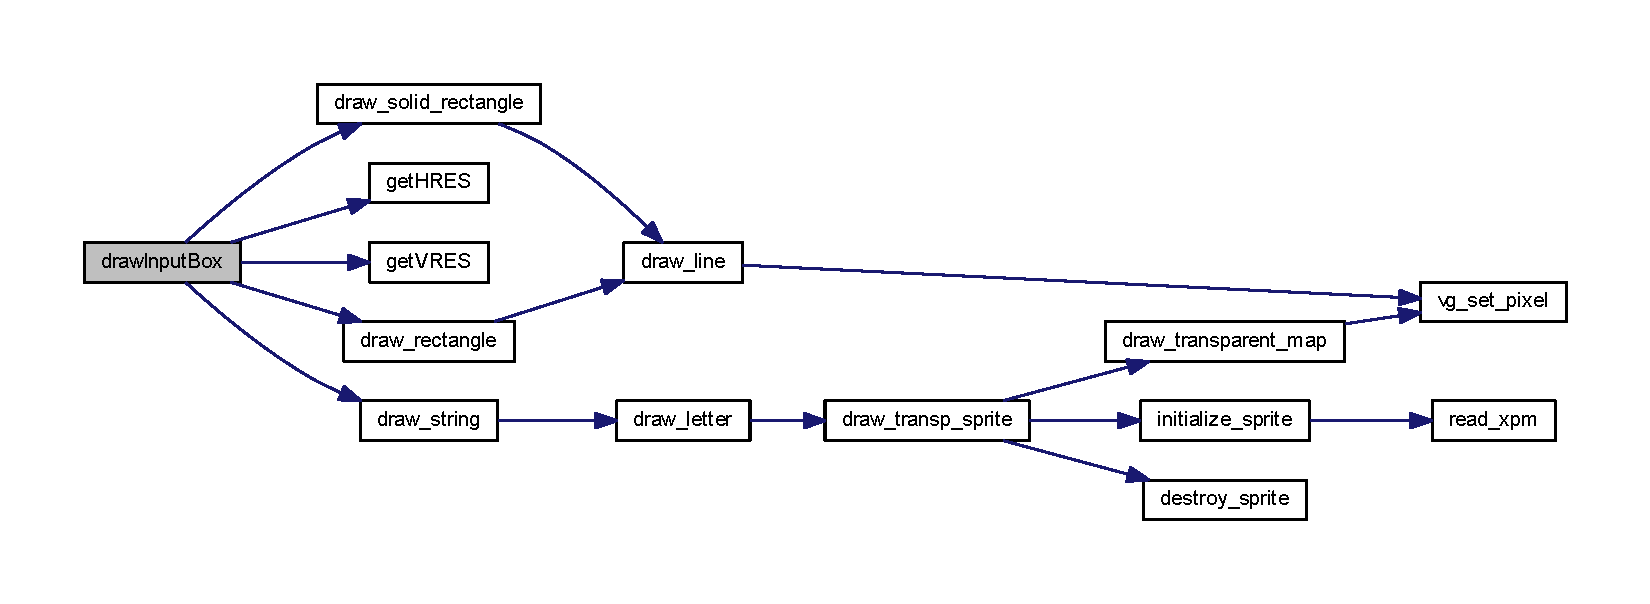
\includegraphics[width=350pt]{interface_8h_a6f3710a0deef4dec8c40e1387f00b2cf_cgraph}
\end{center}
\end{figure}


\hypertarget{interface_8h_a06326bc3ce2fdfe90cb6eb3172159fd0}{}\index{interface.\+h@{interface.\+h}!draw\+Main\+Menu@{draw\+Main\+Menu}}
\index{draw\+Main\+Menu@{draw\+Main\+Menu}!interface.\+h@{interface.\+h}}
\subsubsection[{draw\+Main\+Menu}]{\setlength{\rightskip}{0pt plus 5cm}void draw\+Main\+Menu (
\begin{DoxyParamCaption}
{}
\end{DoxyParamCaption}
)}\label{interface_8h_a06326bc3ce2fdfe90cb6eb3172159fd0}
Draws main menu 

Definition at line 46 of file interface.\+c.



Here is the call graph for this function\+:\nopagebreak
\begin{figure}[H]
\begin{center}
\leavevmode
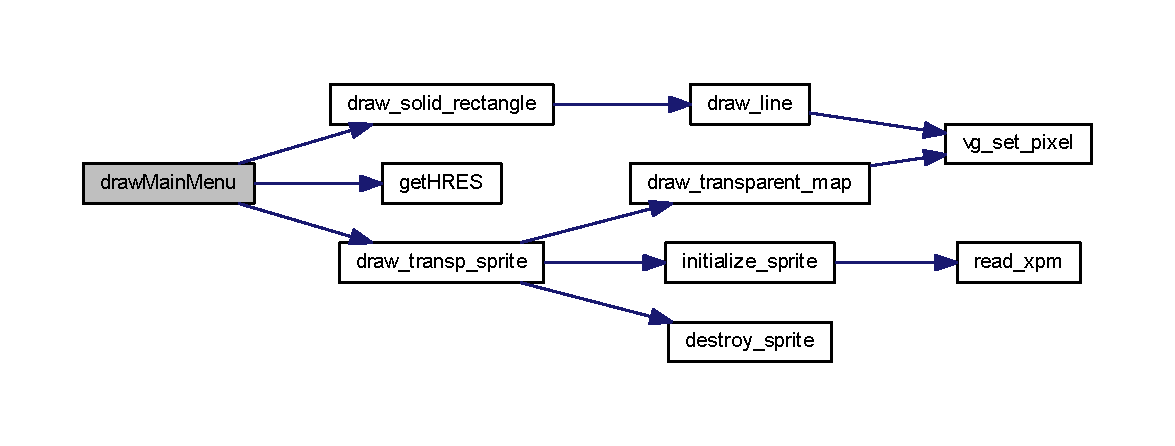
\includegraphics[width=350pt]{interface_8h_a06326bc3ce2fdfe90cb6eb3172159fd0_cgraph}
\end{center}
\end{figure}


\hypertarget{interface_8h_a04b43cf8b4fbf16e17cea07e7daf8bf9}{}\index{interface.\+h@{interface.\+h}!draw\+Output\+Box@{draw\+Output\+Box}}
\index{draw\+Output\+Box@{draw\+Output\+Box}!interface.\+h@{interface.\+h}}
\subsubsection[{draw\+Output\+Box}]{\setlength{\rightskip}{0pt plus 5cm}void draw\+Output\+Box (
\begin{DoxyParamCaption}
\item[{char $\ast$}]{title, }
\item[{char $\ast$}]{message}
\end{DoxyParamCaption}
)}\label{interface_8h_a04b43cf8b4fbf16e17cea07e7daf8bf9}
Draws a pop-\/up box with title and message 
\begin{DoxyParams}{Parameters}
{\em title} & \\
\hline
{\em message} & \\
\hline
\end{DoxyParams}


Definition at line 84 of file interface.\+c.



Here is the call graph for this function\+:\nopagebreak
\begin{figure}[H]
\begin{center}
\leavevmode
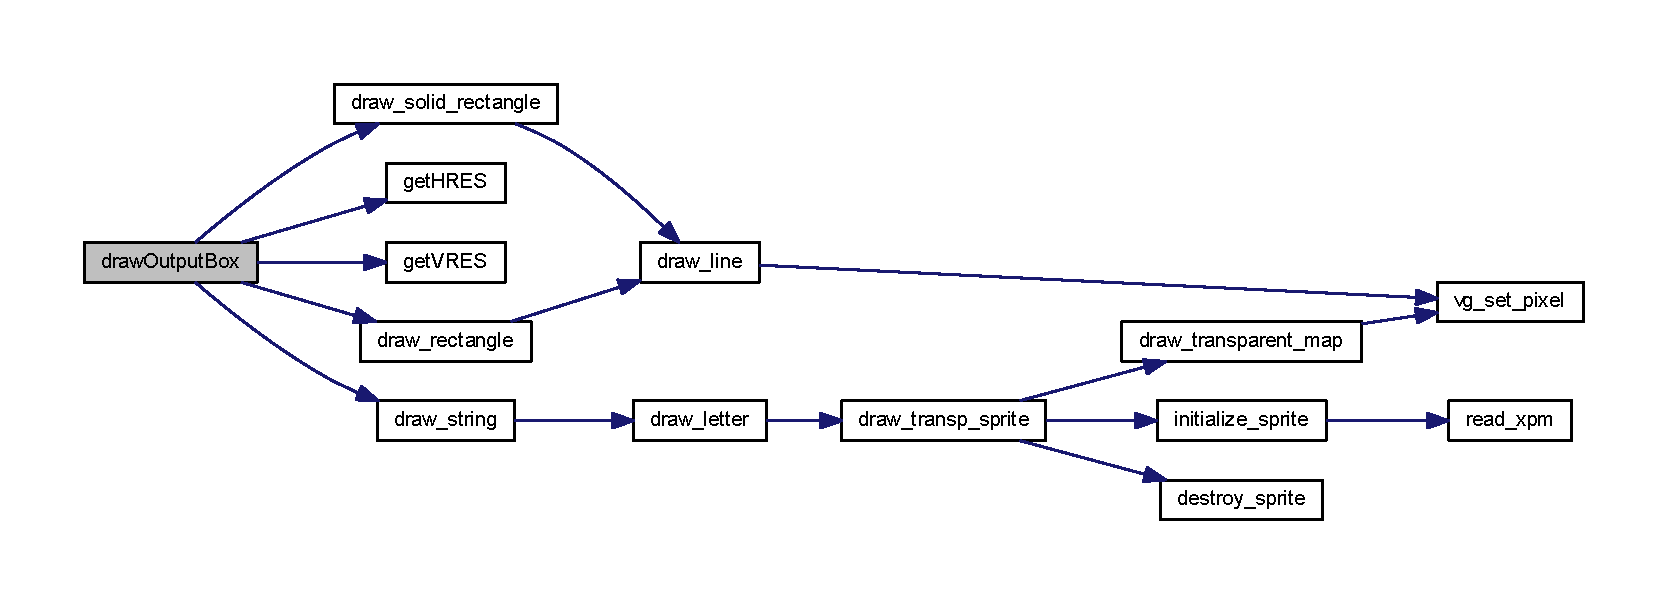
\includegraphics[width=350pt]{interface_8h_a04b43cf8b4fbf16e17cea07e7daf8bf9_cgraph}
\end{center}
\end{figure}


\hypertarget{interface_8h_a7191ba49f3495cfb9304adc2a6661d7e}{}\index{interface.\+h@{interface.\+h}!draw\+Right\+Click\+Menu@{draw\+Right\+Click\+Menu}}
\index{draw\+Right\+Click\+Menu@{draw\+Right\+Click\+Menu}!interface.\+h@{interface.\+h}}
\subsubsection[{draw\+Right\+Click\+Menu}]{\setlength{\rightskip}{0pt plus 5cm}void draw\+Right\+Click\+Menu (
\begin{DoxyParamCaption}
\item[{{\bf mouse\+\_\+state}}]{current\+\_\+mouse\+\_\+state}
\end{DoxyParamCaption}
)}\label{interface_8h_a7191ba49f3495cfb9304adc2a6661d7e}
Draws right click menu according to \hyperlink{structmouse__state}{mouse\+\_\+state} coordinates 
\begin{DoxyParams}{Parameters}
{\em current\+\_\+mouse\+\_\+state} & \\
\hline
\end{DoxyParams}


Definition at line 247 of file interface.\+c.



Here is the call graph for this function\+:\nopagebreak
\begin{figure}[H]
\begin{center}
\leavevmode
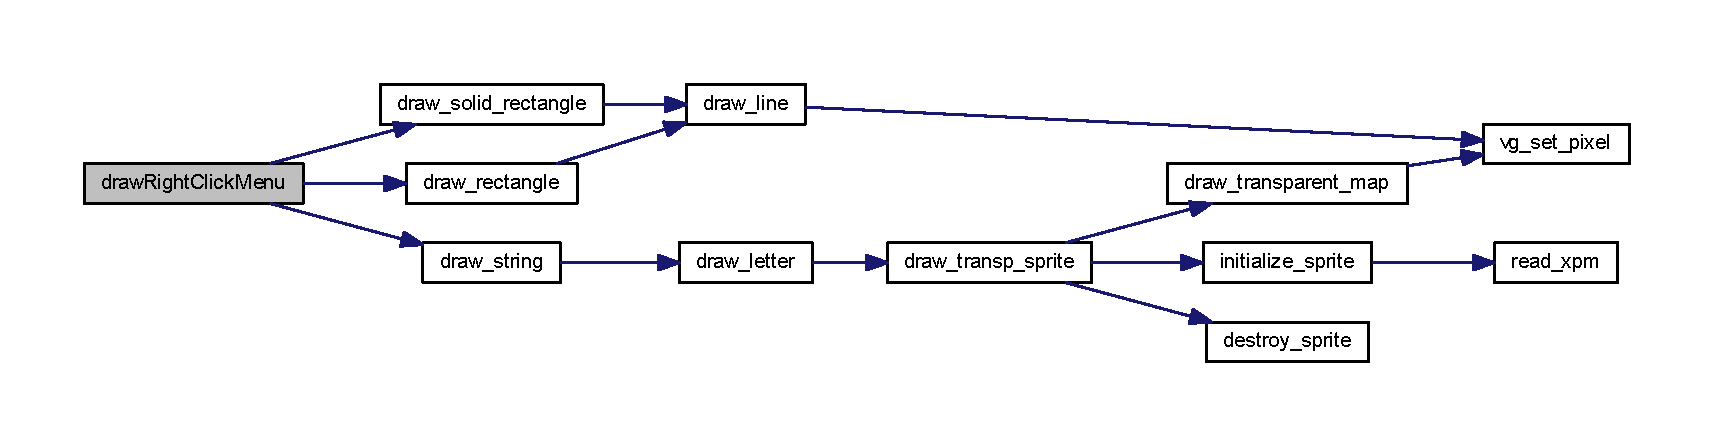
\includegraphics[width=350pt]{interface_8h_a7191ba49f3495cfb9304adc2a6661d7e_cgraph}
\end{center}
\end{figure}


\hypertarget{interface_8h_aaee65a42f436525f7b9887fbe4f3663d}{}\index{interface.\+h@{interface.\+h}!main\+Draw@{main\+Draw}}
\index{main\+Draw@{main\+Draw}!interface.\+h@{interface.\+h}}
\subsubsection[{main\+Draw}]{\setlength{\rightskip}{0pt plus 5cm}void main\+Draw (
\begin{DoxyParamCaption}
{}
\end{DoxyParamCaption}
)}\label{interface_8h_aaee65a42f436525f7b9887fbe4f3663d}
Draws the initial interface (Penguin, logo and developers) 

Definition at line 7 of file interface.\+c.



Here is the call graph for this function\+:\nopagebreak
\begin{figure}[H]
\begin{center}
\leavevmode
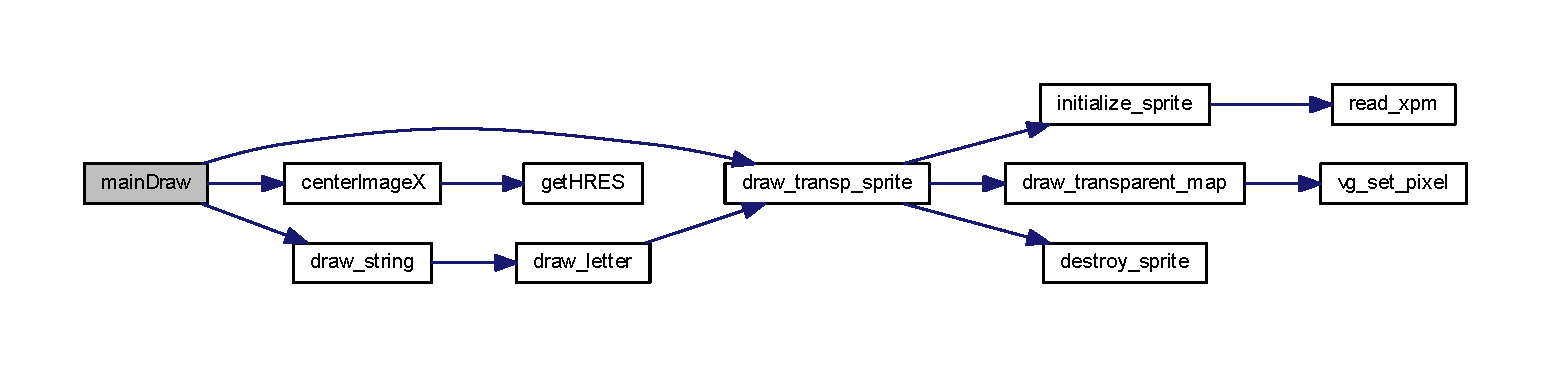
\includegraphics[width=350pt]{interface_8h_aaee65a42f436525f7b9887fbe4f3663d_cgraph}
\end{center}
\end{figure}



\hypertarget{keyboard_8c}{}\section{keyboard.\+c File Reference}
\label{keyboard_8c}\index{keyboard.\+c@{keyboard.\+c}}
{\ttfamily \#include \char`\"{}keyboard.\+h\char`\"{}}\\*
\subsection*{Functions}
\begin{DoxyCompactItemize}
\item 
void \hyperlink{keyboard_8c_af9d4827856b96cc09dc19308771fcd24}{set\+Timer\+Flag} ()
\item 
void \hyperlink{keyboard_8c_aa022a30b37ac135bdebcf64b6787e621}{set\+Assembly\+Flag} ()
\item 
void \hyperlink{keyboard_8c_a538a48fcda412eebfedbf8e5b45397a9}{set\+Time} (int seconds)
\item 
int \hyperlink{keyboard_8c_aa6ca41cf20ce933ec9bbd56b193278cc}{keyboard\+\_\+subscribe\+\_\+int} (void)
\item 
int \hyperlink{keyboard_8c_ac95aea27a5e91b363b876fed881f368f}{keyboard\+\_\+unsubscribe\+\_\+int} ()
\item 
int \hyperlink{keyboard_8c_ab07cf29ed086faf6d5a30e0c7cd443e2}{keyboard\+\_\+int\+\_\+handler\+\_\+\+C} (unsigned long $\ast$code)
\item 
void \hyperlink{keyboard_8c_a4c24e4a8939cfda0f96ebafcf0d8b0a6}{print\+\_\+codes} (unsigned long code)
\item 
int \hyperlink{keyboard_8c_a8c04882e56f7ceb7257ba13e0652b188}{receiver\+\_\+loop} (int shiftkeyboard)
\item 
int \hyperlink{keyboard_8c_a16755b6adaea6823bf15eb00344deb08}{issue\+\_\+command} (unsigned long command, unsigned long argument)
\end{DoxyCompactItemize}


\subsection{Function Documentation}
\hypertarget{keyboard_8c_a16755b6adaea6823bf15eb00344deb08}{}\index{keyboard.\+c@{keyboard.\+c}!issue\+\_\+command@{issue\+\_\+command}}
\index{issue\+\_\+command@{issue\+\_\+command}!keyboard.\+c@{keyboard.\+c}}
\subsubsection[{issue\+\_\+command}]{\setlength{\rightskip}{0pt plus 5cm}int issue\+\_\+command (
\begin{DoxyParamCaption}
\item[{unsigned long}]{command, }
\item[{unsigned long}]{argument}
\end{DoxyParamCaption}
)}\label{keyboard_8c_a16755b6adaea6823bf15eb00344deb08}


Definition at line 127 of file keyboard.\+c.

\hypertarget{keyboard_8c_ab07cf29ed086faf6d5a30e0c7cd443e2}{}\index{keyboard.\+c@{keyboard.\+c}!keyboard\+\_\+int\+\_\+handler\+\_\+\+C@{keyboard\+\_\+int\+\_\+handler\+\_\+\+C}}
\index{keyboard\+\_\+int\+\_\+handler\+\_\+\+C@{keyboard\+\_\+int\+\_\+handler\+\_\+\+C}!keyboard.\+c@{keyboard.\+c}}
\subsubsection[{keyboard\+\_\+int\+\_\+handler\+\_\+\+C}]{\setlength{\rightskip}{0pt plus 5cm}int keyboard\+\_\+int\+\_\+handler\+\_\+\+C (
\begin{DoxyParamCaption}
\item[{unsigned long $\ast$}]{code}
\end{DoxyParamCaption}
)}\label{keyboard_8c_ab07cf29ed086faf6d5a30e0c7cd443e2}
Handles interrupts for the keyboard 

Definition at line 29 of file keyboard.\+c.

\hypertarget{keyboard_8c_aa6ca41cf20ce933ec9bbd56b193278cc}{}\index{keyboard.\+c@{keyboard.\+c}!keyboard\+\_\+subscribe\+\_\+int@{keyboard\+\_\+subscribe\+\_\+int}}
\index{keyboard\+\_\+subscribe\+\_\+int@{keyboard\+\_\+subscribe\+\_\+int}!keyboard.\+c@{keyboard.\+c}}
\subsubsection[{keyboard\+\_\+subscribe\+\_\+int}]{\setlength{\rightskip}{0pt plus 5cm}int keyboard\+\_\+subscribe\+\_\+int (
\begin{DoxyParamCaption}
{}
\end{DoxyParamCaption}
)}\label{keyboard_8c_aa6ca41cf20ce933ec9bbd56b193278cc}
Subscribes keyboard interrupts 

Definition at line 15 of file keyboard.\+c.

\hypertarget{keyboard_8c_ac95aea27a5e91b363b876fed881f368f}{}\index{keyboard.\+c@{keyboard.\+c}!keyboard\+\_\+unsubscribe\+\_\+int@{keyboard\+\_\+unsubscribe\+\_\+int}}
\index{keyboard\+\_\+unsubscribe\+\_\+int@{keyboard\+\_\+unsubscribe\+\_\+int}!keyboard.\+c@{keyboard.\+c}}
\subsubsection[{keyboard\+\_\+unsubscribe\+\_\+int}]{\setlength{\rightskip}{0pt plus 5cm}int keyboard\+\_\+unsubscribe\+\_\+int (
\begin{DoxyParamCaption}
{}
\end{DoxyParamCaption}
)}\label{keyboard_8c_ac95aea27a5e91b363b876fed881f368f}
Unsubscribes keyboard interrupts 

Definition at line 22 of file keyboard.\+c.

\hypertarget{keyboard_8c_a4c24e4a8939cfda0f96ebafcf0d8b0a6}{}\index{keyboard.\+c@{keyboard.\+c}!print\+\_\+codes@{print\+\_\+codes}}
\index{print\+\_\+codes@{print\+\_\+codes}!keyboard.\+c@{keyboard.\+c}}
\subsubsection[{print\+\_\+codes}]{\setlength{\rightskip}{0pt plus 5cm}void print\+\_\+codes (
\begin{DoxyParamCaption}
\item[{unsigned long}]{code}
\end{DoxyParamCaption}
)}\label{keyboard_8c_a4c24e4a8939cfda0f96ebafcf0d8b0a6}
Prints keyboard input codes 

Definition at line 79 of file keyboard.\+c.

\hypertarget{keyboard_8c_a8c04882e56f7ceb7257ba13e0652b188}{}\index{keyboard.\+c@{keyboard.\+c}!receiver\+\_\+loop@{receiver\+\_\+loop}}
\index{receiver\+\_\+loop@{receiver\+\_\+loop}!keyboard.\+c@{keyboard.\+c}}
\subsubsection[{receiver\+\_\+loop}]{\setlength{\rightskip}{0pt plus 5cm}int receiver\+\_\+loop (
\begin{DoxyParamCaption}
\item[{int}]{shiftkeyboard}
\end{DoxyParamCaption}
)}\label{keyboard_8c_a8c04882e56f7ceb7257ba13e0652b188}


Definition at line 91 of file keyboard.\+c.



Here is the call graph for this function\+:\nopagebreak
\begin{figure}[H]
\begin{center}
\leavevmode
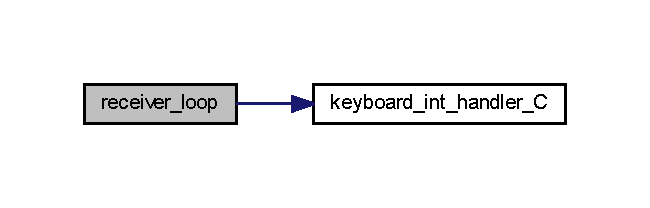
\includegraphics[width=312pt]{keyboard_8c_a8c04882e56f7ceb7257ba13e0652b188_cgraph}
\end{center}
\end{figure}


\hypertarget{keyboard_8c_aa022a30b37ac135bdebcf64b6787e621}{}\index{keyboard.\+c@{keyboard.\+c}!set\+Assembly\+Flag@{set\+Assembly\+Flag}}
\index{set\+Assembly\+Flag@{set\+Assembly\+Flag}!keyboard.\+c@{keyboard.\+c}}
\subsubsection[{set\+Assembly\+Flag}]{\setlength{\rightskip}{0pt plus 5cm}void set\+Assembly\+Flag (
\begin{DoxyParamCaption}
{}
\end{DoxyParamCaption}
)}\label{keyboard_8c_aa022a30b37ac135bdebcf64b6787e621}


Definition at line 7 of file keyboard.\+c.

\hypertarget{keyboard_8c_a538a48fcda412eebfedbf8e5b45397a9}{}\index{keyboard.\+c@{keyboard.\+c}!set\+Time@{set\+Time}}
\index{set\+Time@{set\+Time}!keyboard.\+c@{keyboard.\+c}}
\subsubsection[{set\+Time}]{\setlength{\rightskip}{0pt plus 5cm}void set\+Time (
\begin{DoxyParamCaption}
\item[{int}]{seconds}
\end{DoxyParamCaption}
)}\label{keyboard_8c_a538a48fcda412eebfedbf8e5b45397a9}
Set seconds 

Definition at line 11 of file keyboard.\+c.

\hypertarget{keyboard_8c_af9d4827856b96cc09dc19308771fcd24}{}\index{keyboard.\+c@{keyboard.\+c}!set\+Timer\+Flag@{set\+Timer\+Flag}}
\index{set\+Timer\+Flag@{set\+Timer\+Flag}!keyboard.\+c@{keyboard.\+c}}
\subsubsection[{set\+Timer\+Flag}]{\setlength{\rightskip}{0pt plus 5cm}void set\+Timer\+Flag (
\begin{DoxyParamCaption}
{}
\end{DoxyParamCaption}
)}\label{keyboard_8c_af9d4827856b96cc09dc19308771fcd24}
Activate timer flag 

Definition at line 3 of file keyboard.\+c.


\hypertarget{keyboard_8h}{}\section{keyboard.\+h File Reference}
\label{keyboard_8h}\index{keyboard.\+h@{keyboard.\+h}}
{\ttfamily \#include $<$minix/syslib.\+h$>$}\\*
{\ttfamily \#include $<$minix/drivers.\+h$>$}\\*
{\ttfamily \#include \char`\"{}headers.\+h\char`\"{}}\\*
{\ttfamily \#include \char`\"{}i8254.\+h\char`\"{}}\\*
{\ttfamily \#include \char`\"{}timer.\+h\char`\"{}}\\*
\subsection*{Functions}
\begin{DoxyCompactItemize}
\item 
void \hyperlink{keyboard_8h_af9d4827856b96cc09dc19308771fcd24}{set\+Timer\+Flag} ()
\item 
void \hyperlink{keyboard_8h_a538a48fcda412eebfedbf8e5b45397a9}{set\+Time} (int seconds)
\item 
int \hyperlink{keyboard_8h_ab07cf29ed086faf6d5a30e0c7cd443e2}{keyboard\+\_\+int\+\_\+handler\+\_\+\+C} (unsigned long $\ast$code)
\item 
int \hyperlink{keyboard_8h_a4ac76b0a9a73670254d5fd4c520e458f}{keyboard\+\_\+subscribe\+\_\+int} ()
\item 
int \hyperlink{keyboard_8h_ac95aea27a5e91b363b876fed881f368f}{keyboard\+\_\+unsubscribe\+\_\+int} ()
\item 
int \hyperlink{keyboard_8h_a16755b6adaea6823bf15eb00344deb08}{issue\+\_\+command} (unsigned long command, unsigned long argument)
\item 
int \hyperlink{keyboard_8h_af94b6d9ab910f1571cfe57854870b083}{receiver\+\_\+loop} ()
\item 
void \hyperlink{keyboard_8h_a4c24e4a8939cfda0f96ebafcf0d8b0a6}{print\+\_\+codes} (unsigned long code)
\end{DoxyCompactItemize}


\subsection{Function Documentation}
\hypertarget{keyboard_8h_a16755b6adaea6823bf15eb00344deb08}{}\index{keyboard.\+h@{keyboard.\+h}!issue\+\_\+command@{issue\+\_\+command}}
\index{issue\+\_\+command@{issue\+\_\+command}!keyboard.\+h@{keyboard.\+h}}
\subsubsection[{issue\+\_\+command}]{\setlength{\rightskip}{0pt plus 5cm}int issue\+\_\+command (
\begin{DoxyParamCaption}
\item[{unsigned long}]{command, }
\item[{unsigned long}]{argument}
\end{DoxyParamCaption}
)}\label{keyboard_8h_a16755b6adaea6823bf15eb00344deb08}


Definition at line 127 of file keyboard.\+c.

\hypertarget{keyboard_8h_ab07cf29ed086faf6d5a30e0c7cd443e2}{}\index{keyboard.\+h@{keyboard.\+h}!keyboard\+\_\+int\+\_\+handler\+\_\+\+C@{keyboard\+\_\+int\+\_\+handler\+\_\+\+C}}
\index{keyboard\+\_\+int\+\_\+handler\+\_\+\+C@{keyboard\+\_\+int\+\_\+handler\+\_\+\+C}!keyboard.\+h@{keyboard.\+h}}
\subsubsection[{keyboard\+\_\+int\+\_\+handler\+\_\+\+C}]{\setlength{\rightskip}{0pt plus 5cm}int keyboard\+\_\+int\+\_\+handler\+\_\+\+C (
\begin{DoxyParamCaption}
\item[{unsigned long $\ast$}]{code}
\end{DoxyParamCaption}
)}\label{keyboard_8h_ab07cf29ed086faf6d5a30e0c7cd443e2}
Handles interrupts for the keyboard 

Definition at line 29 of file keyboard.\+c.

\hypertarget{keyboard_8h_a4ac76b0a9a73670254d5fd4c520e458f}{}\index{keyboard.\+h@{keyboard.\+h}!keyboard\+\_\+subscribe\+\_\+int@{keyboard\+\_\+subscribe\+\_\+int}}
\index{keyboard\+\_\+subscribe\+\_\+int@{keyboard\+\_\+subscribe\+\_\+int}!keyboard.\+h@{keyboard.\+h}}
\subsubsection[{keyboard\+\_\+subscribe\+\_\+int}]{\setlength{\rightskip}{0pt plus 5cm}int keyboard\+\_\+subscribe\+\_\+int (
\begin{DoxyParamCaption}
{}
\end{DoxyParamCaption}
)}\label{keyboard_8h_a4ac76b0a9a73670254d5fd4c520e458f}
Subscribes keyboard interrupts 

Definition at line 15 of file keyboard.\+c.

\hypertarget{keyboard_8h_ac95aea27a5e91b363b876fed881f368f}{}\index{keyboard.\+h@{keyboard.\+h}!keyboard\+\_\+unsubscribe\+\_\+int@{keyboard\+\_\+unsubscribe\+\_\+int}}
\index{keyboard\+\_\+unsubscribe\+\_\+int@{keyboard\+\_\+unsubscribe\+\_\+int}!keyboard.\+h@{keyboard.\+h}}
\subsubsection[{keyboard\+\_\+unsubscribe\+\_\+int}]{\setlength{\rightskip}{0pt plus 5cm}int keyboard\+\_\+unsubscribe\+\_\+int (
\begin{DoxyParamCaption}
{}
\end{DoxyParamCaption}
)}\label{keyboard_8h_ac95aea27a5e91b363b876fed881f368f}
Unsubscribes keyboard interrupts 

Definition at line 22 of file keyboard.\+c.

\hypertarget{keyboard_8h_a4c24e4a8939cfda0f96ebafcf0d8b0a6}{}\index{keyboard.\+h@{keyboard.\+h}!print\+\_\+codes@{print\+\_\+codes}}
\index{print\+\_\+codes@{print\+\_\+codes}!keyboard.\+h@{keyboard.\+h}}
\subsubsection[{print\+\_\+codes}]{\setlength{\rightskip}{0pt plus 5cm}void print\+\_\+codes (
\begin{DoxyParamCaption}
\item[{unsigned long}]{code}
\end{DoxyParamCaption}
)}\label{keyboard_8h_a4c24e4a8939cfda0f96ebafcf0d8b0a6}
Prints keyboard input codes 

Definition at line 79 of file keyboard.\+c.

\hypertarget{keyboard_8h_af94b6d9ab910f1571cfe57854870b083}{}\index{keyboard.\+h@{keyboard.\+h}!receiver\+\_\+loop@{receiver\+\_\+loop}}
\index{receiver\+\_\+loop@{receiver\+\_\+loop}!keyboard.\+h@{keyboard.\+h}}
\subsubsection[{receiver\+\_\+loop}]{\setlength{\rightskip}{0pt plus 5cm}int receiver\+\_\+loop (
\begin{DoxyParamCaption}
{}
\end{DoxyParamCaption}
)}\label{keyboard_8h_af94b6d9ab910f1571cfe57854870b083}
Loop to handle keyboard interrupts \hypertarget{keyboard_8h_a538a48fcda412eebfedbf8e5b45397a9}{}\index{keyboard.\+h@{keyboard.\+h}!set\+Time@{set\+Time}}
\index{set\+Time@{set\+Time}!keyboard.\+h@{keyboard.\+h}}
\subsubsection[{set\+Time}]{\setlength{\rightskip}{0pt plus 5cm}void set\+Time (
\begin{DoxyParamCaption}
\item[{int}]{seconds}
\end{DoxyParamCaption}
)}\label{keyboard_8h_a538a48fcda412eebfedbf8e5b45397a9}
Set seconds 

Definition at line 11 of file keyboard.\+c.

\hypertarget{keyboard_8h_af9d4827856b96cc09dc19308771fcd24}{}\index{keyboard.\+h@{keyboard.\+h}!set\+Timer\+Flag@{set\+Timer\+Flag}}
\index{set\+Timer\+Flag@{set\+Timer\+Flag}!keyboard.\+h@{keyboard.\+h}}
\subsubsection[{set\+Timer\+Flag}]{\setlength{\rightskip}{0pt plus 5cm}void set\+Timer\+Flag (
\begin{DoxyParamCaption}
{}
\end{DoxyParamCaption}
)}\label{keyboard_8h_af9d4827856b96cc09dc19308771fcd24}
Activate timer flag 

Definition at line 3 of file keyboard.\+c.


\hypertarget{lmlib_8h}{}\section{lmlib.\+h File Reference}
\label{lmlib_8h}\index{lmlib.\+h@{lmlib.\+h}}
\subsection*{Classes}
\begin{DoxyCompactItemize}
\item 
struct \hyperlink{structmmap__t}{mmap\+\_\+t}
\end{DoxyCompactItemize}
\subsection*{Functions}
\begin{DoxyCompactItemize}
\item 
void $\ast$ \hyperlink{group__lmlib_ga00a9c17c01e794a6bfc80fc5c6ab1ed1}{lm\+\_\+init} (void)
\begin{DoxyCompactList}\small\item\em Initializes the low memory area, the region up to the 1 M\+Byte physical address, by mapping it on the process\textquotesingle{} physical memory address. \end{DoxyCompactList}\item 
void $\ast$ \hyperlink{group__lmlib_gae45d971ce2ffcf4dc2677eba033a92cd}{lm\+\_\+alloc} (unsigned long size, \hyperlink{structmmap__t}{mmap\+\_\+t} $\ast$map)
\begin{DoxyCompactList}\small\item\em Allocates a memory block in low memory area with the specified size. \end{DoxyCompactList}\item 
void \hyperlink{group__lmlib_ga73e89d9c297b7390021fb545513579c6}{lm\+\_\+free} (\hyperlink{structmmap__t}{mmap\+\_\+t} $\ast$map)
\begin{DoxyCompactList}\small\item\em Frees a memory block in the low memory area, previously allocated using \hyperlink{group__lmlib_gae45d971ce2ffcf4dc2677eba033a92cd}{lm\+\_\+alloc()} \end{DoxyCompactList}\end{DoxyCompactItemize}

\hypertarget{logic_8c}{}\section{logic.\+c File Reference}
\label{logic_8c}\index{logic.\+c@{logic.\+c}}
{\ttfamily \#include \char`\"{}logic.\+h\char`\"{}}\\*
{\ttfamily \#include $<$stdio.\+h$>$}\\*
{\ttfamily \#include $<$stdlib.\+h$>$}\\*
\subsection*{Functions}
\begin{DoxyCompactItemize}
\item 
int \hyperlink{logic_8c_a0a12179d687ca2d67e72e78268f7cc2c}{collision} (\hyperlink{structmouse__state}{mouse\+\_\+state} mouse, \hyperlink{logic_8h_a8dd5b76d2972cdce6fd4f1c7d8e175c5}{Button} a)
\item 
int \hyperlink{logic_8c_aa39071f67e32c2002f72ce59c1e6fa11}{check\+\_\+mouse\+\_\+click} (\hyperlink{structmouse__state}{mouse\+\_\+state} \hyperlink{state_8h_a39d9a371f9aef2042923a96e2f855d5e}{current\+\_\+mouse\+\_\+state})
\item 
void \hyperlink{logic_8c_a27d3ba5afb772cc36c9a432c28975ace}{init\+Buttons} ()
\item 
int \hyperlink{logic_8c_ab16ca2694321ab91f2f0a0b332c0df58}{check\+\_\+mouse\+\_\+double\+\_\+click} (\hyperlink{structmouse__state}{mouse\+\_\+state} \hyperlink{state_8h_a39d9a371f9aef2042923a96e2f855d5e}{current\+\_\+mouse\+\_\+state})
\item 
void \hyperlink{logic_8c_a737abc4763c06db503f514a639fea08c}{check\+\_\+rename\+\_\+folder} ()
\item 
int \hyperlink{logic_8c_ac4ac4a95ff10cf3256c2a36d0e90d45e}{check\+\_\+delete\+\_\+files} ()
\item 
void \hyperlink{logic_8c_a20a866a30fdbb32fc9bfc74dacd0b89c}{set\+Delete\+Flag} ()
\item 
int \hyperlink{logic_8c_aaa9525bb143ec0e36c7b6eda42881715}{get\+Delete\+Flag} ()
\item 
int \hyperlink{logic_8c_a283e5fd540509ad3e89cd63bb7f6e999}{get\+Turn\+Off\+Flag} ()
\item 
void \hyperlink{logic_8c_a6673774c3b7ef292567a5637f47a9579}{set\+Rename\+Flag} ()
\item 
int \hyperlink{logic_8c_a62436370dd4c3bd2452cef7f4fd7b7f0}{get\+Rename\+Flag} ()
\item 
int \hyperlink{logic_8c_a0e1eda02d10d0930fa24e87170c111ff}{is\+Box\+Confirmed} ()
\item 
void \hyperlink{logic_8c_a913ad8296c70b807df4fbf6302f8072a}{open\+Folder} (int index)
\item 
void \hyperlink{logic_8c_a0d8e78acd24989789082f4306f903596}{disable\+Box} ()
\item 
void \hyperlink{logic_8c_a017ced8b7330e5d2522c9718de024750}{enable\+Box} (int type, char $\ast$title, char $\ast$text)
\item 
char $\ast$ \hyperlink{logic_8c_ac767299fe51a7511dc7dcb8f41a1f4b9}{get\+Box\+Title} ()
\item 
char $\ast$ \hyperlink{logic_8c_a158bfa83c4b1dd186a3a89151b687e01}{get\+Box\+Text} ()
\item 
int \hyperlink{logic_8c_a7400b316b1eb9244af06ab06f37757f8}{is\+Box} ()
\item 
int \hyperlink{logic_8c_a7b844fdb59d5c51e10bceedf336b6429}{is\+Output} ()
\item 
char $\ast$ \hyperlink{logic_8c_a87d8b4ed67ed030ef2f6f3faeb7aa6df}{get\+Title} ()
\item 
void \hyperlink{logic_8c_a530fba246396179676ecb402fb2d2e4a}{delete\+Folder} (int index)
\item 
void \hyperlink{logic_8c_a1e48323b0a3fdd311f7cd1988532ace8}{rename\+Folder} (int index)
\item 
int \hyperlink{logic_8c_ab8591ddf31e5c4ab28c07160e84ee893}{navigate\+Left} ()
\item 
int \hyperlink{logic_8c_a87b6ad8fb397f0e72cbf79c99c3c3b25}{navigate\+Right} ()
\item 
int \hyperlink{logic_8c_ade9da36feece104d5099779b77e0370d}{navigate\+Up} ()
\item 
int \hyperlink{logic_8c_a602ddea367dab1b4fec0e9f96abbcf0f}{navigate\+Down} ()
\item 
char $\ast$ \hyperlink{logic_8c_a31ba4de847c8b9762dfe9fdbb08ef4f1}{get\+Folder\+Name} (int index)
\item 
int \hyperlink{logic_8c_a34121a3403c30a9dd71f71624aaaf0e7}{is\+Folder\+Selected} (int index)
\item 
int \hyperlink{logic_8c_a317bd44d55f4edc8580bbdbdc8a5f506}{open\+Folder\+By\+Enter} ()
\item 
int \hyperlink{logic_8c_a6ea97012f3e7cfbdac36a77b25046e9b}{move\+Back} ()
\item 
int \hyperlink{logic_8c_a4ea80b22f633b3030dec0db2269ada1d}{get\+Folder\+Selected} ()
\item 
void \hyperlink{logic_8c_a3b3c14dae824723e0e1b4720a370b3e6}{set\+Folder\+Coords} (int index, int in\+X, int in\+Y)
\item 
void \hyperlink{logic_8c_aa9f20f8c541306d3b93879d0a6d497e8}{toggle\+Selected} (int index)
\item 
char $\ast$ \hyperlink{logic_8c_a551b12c420e086648c320df4fa034130}{get\+Path} ()
\item 
\hyperlink{logic_8h_ad5e554666c5d1a199d39416c639f97f8}{Directory} $\ast$ \hyperlink{logic_8c_a4b7468f1ca81496cf0ee00452194e81f}{get\+Directories} ()
\item 
int \hyperlink{logic_8c_a00fee6141a63232b663143211aacc392}{get\+Number\+Folders} ()
\item 
int \hyperlink{logic_8c_a65b0f047568e3d106306bd405b5be72b}{get\+Folder\+By\+Coords} (int x, int y)
\item 
char \hyperlink{logic_8c_aa5aa39c1f1818cfbd5141e37c3a9e5c0}{get\+Char\+By\+Number} (unsigned long input)
\item 
void \hyperlink{logic_8c_a501609335890024a00bc939c19538b0f}{update\+Text\+Box} (unsigned long input)
\item 
int \hyperlink{logic_8c_a4b6ed6ccee9c7d03c7f1c93b51debcb7}{is\+File\+By\+Index} (int index)
\item 
int \hyperlink{logic_8c_abfbb060a687a19a5ecb65b761bb153c0}{is\+File} (char $\ast$path)
\item 
void \hyperlink{logic_8c_a5b0080e32e3cb075b00c7184ce3f5ad0}{update\+Path} (char $\ast$foldername)
\item 
int \hyperlink{logic_8c_af25edb24b597453fb95c3c2080569bd5}{get\+Sub\+Folders} (char $\ast$foldername)
\end{DoxyCompactItemize}


\subsection{Function Documentation}
\hypertarget{logic_8c_ac4ac4a95ff10cf3256c2a36d0e90d45e}{}\index{logic.\+c@{logic.\+c}!check\+\_\+delete\+\_\+files@{check\+\_\+delete\+\_\+files}}
\index{check\+\_\+delete\+\_\+files@{check\+\_\+delete\+\_\+files}!logic.\+c@{logic.\+c}}
\subsubsection[{check\+\_\+delete\+\_\+files}]{\setlength{\rightskip}{0pt plus 5cm}int check\+\_\+delete\+\_\+files (
\begin{DoxyParamCaption}
{}
\end{DoxyParamCaption}
)}\label{logic_8c_ac4ac4a95ff10cf3256c2a36d0e90d45e}
Deletes selected folder/file 

Definition at line 112 of file logic.\+c.



Here is the call graph for this function\+:\nopagebreak
\begin{figure}[H]
\begin{center}
\leavevmode
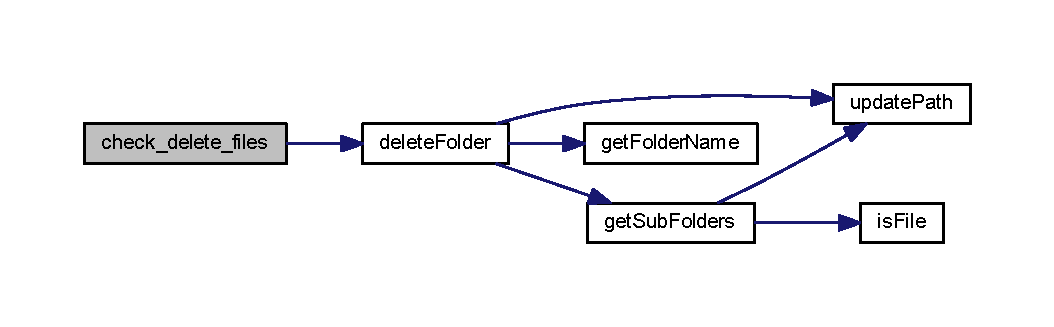
\includegraphics[width=350pt]{logic_8c_ac4ac4a95ff10cf3256c2a36d0e90d45e_cgraph}
\end{center}
\end{figure}


\hypertarget{logic_8c_aa39071f67e32c2002f72ce59c1e6fa11}{}\index{logic.\+c@{logic.\+c}!check\+\_\+mouse\+\_\+click@{check\+\_\+mouse\+\_\+click}}
\index{check\+\_\+mouse\+\_\+click@{check\+\_\+mouse\+\_\+click}!logic.\+c@{logic.\+c}}
\subsubsection[{check\+\_\+mouse\+\_\+click}]{\setlength{\rightskip}{0pt plus 5cm}int check\+\_\+mouse\+\_\+click (
\begin{DoxyParamCaption}
\item[{{\bf mouse\+\_\+state}}]{current\+\_\+mouse\+\_\+state}
\end{DoxyParamCaption}
)}\label{logic_8c_aa39071f67e32c2002f72ce59c1e6fa11}
Does verifications when the mouse is clicked once 
\begin{DoxyParams}{Parameters}
{\em current\+\_\+mouse\+\_\+state} & \\
\hline
\end{DoxyParams}
\begin{DoxyReturn}{Returns}

\end{DoxyReturn}


Definition at line 19 of file logic.\+c.



Here is the call graph for this function\+:\nopagebreak
\begin{figure}[H]
\begin{center}
\leavevmode
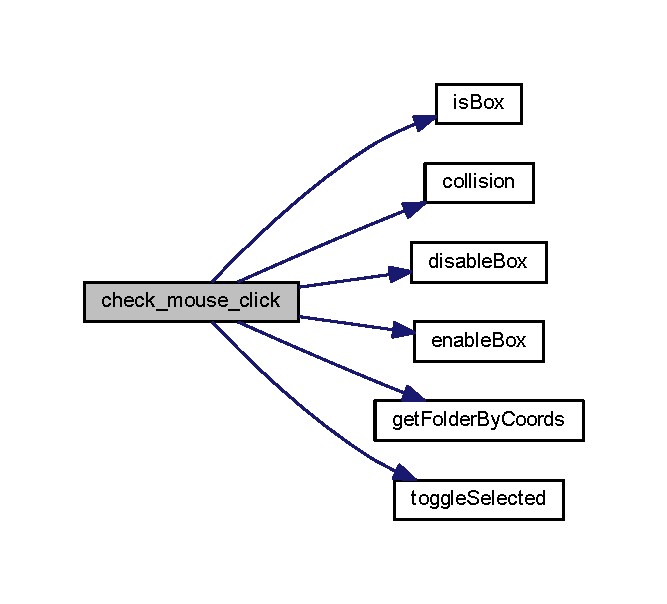
\includegraphics[width=320pt]{logic_8c_aa39071f67e32c2002f72ce59c1e6fa11_cgraph}
\end{center}
\end{figure}


\hypertarget{logic_8c_ab16ca2694321ab91f2f0a0b332c0df58}{}\index{logic.\+c@{logic.\+c}!check\+\_\+mouse\+\_\+double\+\_\+click@{check\+\_\+mouse\+\_\+double\+\_\+click}}
\index{check\+\_\+mouse\+\_\+double\+\_\+click@{check\+\_\+mouse\+\_\+double\+\_\+click}!logic.\+c@{logic.\+c}}
\subsubsection[{check\+\_\+mouse\+\_\+double\+\_\+click}]{\setlength{\rightskip}{0pt plus 5cm}int check\+\_\+mouse\+\_\+double\+\_\+click (
\begin{DoxyParamCaption}
\item[{{\bf mouse\+\_\+state}}]{current\+\_\+mouse\+\_\+state}
\end{DoxyParamCaption}
)}\label{logic_8c_ab16ca2694321ab91f2f0a0b332c0df58}
Does verifications when the mouse is clicked twice in less than 0.\+25 seconds (double click) 
\begin{DoxyParams}{Parameters}
{\em current\+\_\+mouse\+\_\+state} & \\
\hline
\end{DoxyParams}
\begin{DoxyReturn}{Returns}

\end{DoxyReturn}


Definition at line 83 of file logic.\+c.



Here is the call graph for this function\+:\nopagebreak
\begin{figure}[H]
\begin{center}
\leavevmode
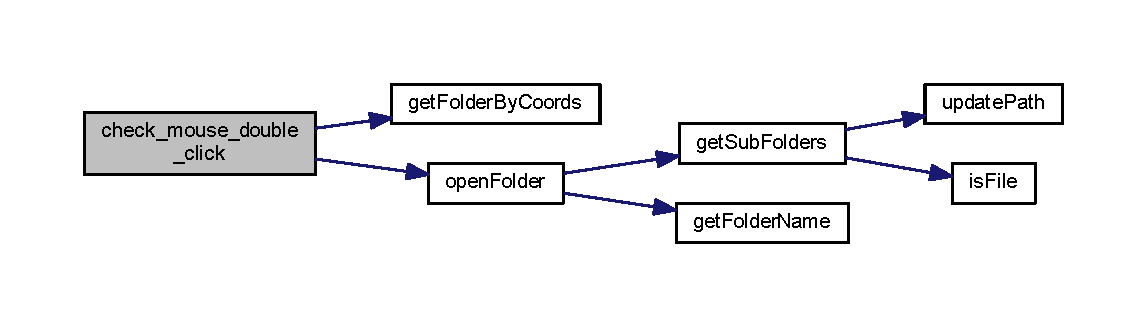
\includegraphics[width=350pt]{logic_8c_ab16ca2694321ab91f2f0a0b332c0df58_cgraph}
\end{center}
\end{figure}


\hypertarget{logic_8c_a737abc4763c06db503f514a639fea08c}{}\index{logic.\+c@{logic.\+c}!check\+\_\+rename\+\_\+folder@{check\+\_\+rename\+\_\+folder}}
\index{check\+\_\+rename\+\_\+folder@{check\+\_\+rename\+\_\+folder}!logic.\+c@{logic.\+c}}
\subsubsection[{check\+\_\+rename\+\_\+folder}]{\setlength{\rightskip}{0pt plus 5cm}void check\+\_\+rename\+\_\+folder (
\begin{DoxyParamCaption}
{}
\end{DoxyParamCaption}
)}\label{logic_8c_a737abc4763c06db503f514a639fea08c}


Definition at line 97 of file logic.\+c.



Here is the call graph for this function\+:\nopagebreak
\begin{figure}[H]
\begin{center}
\leavevmode
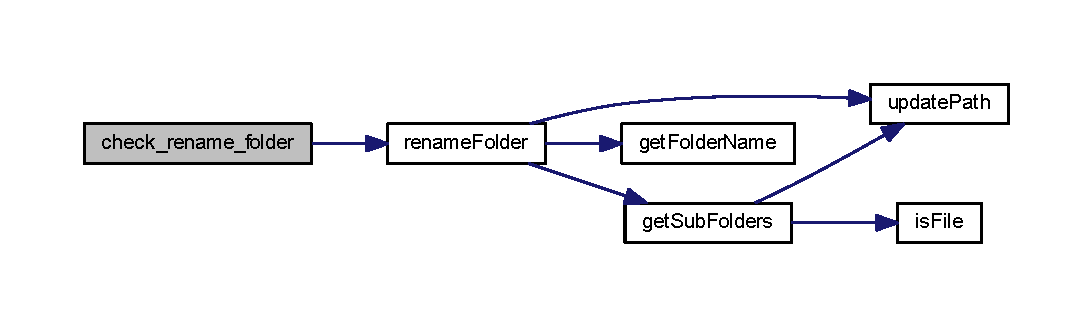
\includegraphics[width=350pt]{logic_8c_a737abc4763c06db503f514a639fea08c_cgraph}
\end{center}
\end{figure}


\hypertarget{logic_8c_a0a12179d687ca2d67e72e78268f7cc2c}{}\index{logic.\+c@{logic.\+c}!collision@{collision}}
\index{collision@{collision}!logic.\+c@{logic.\+c}}
\subsubsection[{collision}]{\setlength{\rightskip}{0pt plus 5cm}int collision (
\begin{DoxyParamCaption}
\item[{{\bf mouse\+\_\+state}}]{mouse, }
\item[{{\bf Button}}]{a}
\end{DoxyParamCaption}
)}\label{logic_8c_a0a12179d687ca2d67e72e78268f7cc2c}
Handles mouse collisions 
\begin{DoxyParams}{Parameters}
{\em mouse} & \\
\hline
{\em a} & \\
\hline
\end{DoxyParams}
\begin{DoxyReturn}{Returns}

\end{DoxyReturn}


Definition at line 8 of file logic.\+c.

\hypertarget{logic_8c_a530fba246396179676ecb402fb2d2e4a}{}\index{logic.\+c@{logic.\+c}!delete\+Folder@{delete\+Folder}}
\index{delete\+Folder@{delete\+Folder}!logic.\+c@{logic.\+c}}
\subsubsection[{delete\+Folder}]{\setlength{\rightskip}{0pt plus 5cm}void delete\+Folder (
\begin{DoxyParamCaption}
\item[{int}]{index}
\end{DoxyParamCaption}
)}\label{logic_8c_a530fba246396179676ecb402fb2d2e4a}
Deletes a folder with a certain index 

Definition at line 198 of file logic.\+c.



Here is the call graph for this function\+:\nopagebreak
\begin{figure}[H]
\begin{center}
\leavevmode
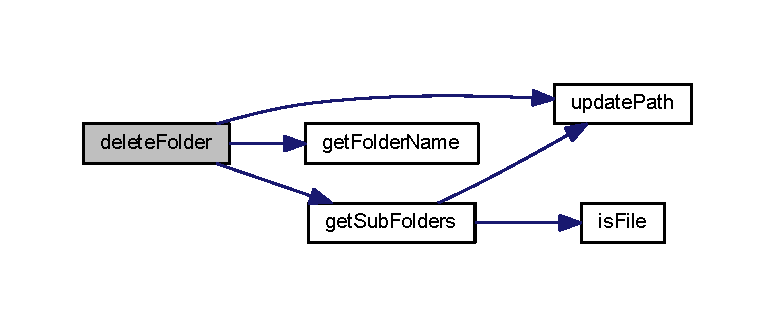
\includegraphics[width=350pt]{logic_8c_a530fba246396179676ecb402fb2d2e4a_cgraph}
\end{center}
\end{figure}


\hypertarget{logic_8c_a0d8e78acd24989789082f4306f903596}{}\index{logic.\+c@{logic.\+c}!disable\+Box@{disable\+Box}}
\index{disable\+Box@{disable\+Box}!logic.\+c@{logic.\+c}}
\subsubsection[{disable\+Box}]{\setlength{\rightskip}{0pt plus 5cm}void disable\+Box (
\begin{DoxyParamCaption}
{}
\end{DoxyParamCaption}
)}\label{logic_8c_a0d8e78acd24989789082f4306f903596}
Disables box 

Definition at line 160 of file logic.\+c.

\hypertarget{logic_8c_a017ced8b7330e5d2522c9718de024750}{}\index{logic.\+c@{logic.\+c}!enable\+Box@{enable\+Box}}
\index{enable\+Box@{enable\+Box}!logic.\+c@{logic.\+c}}
\subsubsection[{enable\+Box}]{\setlength{\rightskip}{0pt plus 5cm}void enable\+Box (
\begin{DoxyParamCaption}
\item[{int}]{type, }
\item[{char $\ast$}]{title, }
\item[{char $\ast$}]{text}
\end{DoxyParamCaption}
)}\label{logic_8c_a017ced8b7330e5d2522c9718de024750}
Enables box 

Definition at line 167 of file logic.\+c.

\hypertarget{logic_8c_a158bfa83c4b1dd186a3a89151b687e01}{}\index{logic.\+c@{logic.\+c}!get\+Box\+Text@{get\+Box\+Text}}
\index{get\+Box\+Text@{get\+Box\+Text}!logic.\+c@{logic.\+c}}
\subsubsection[{get\+Box\+Text}]{\setlength{\rightskip}{0pt plus 5cm}char$\ast$ get\+Box\+Text (
\begin{DoxyParamCaption}
{}
\end{DoxyParamCaption}
)}\label{logic_8c_a158bfa83c4b1dd186a3a89151b687e01}
Gets a box input 

Definition at line 181 of file logic.\+c.

\hypertarget{logic_8c_ac767299fe51a7511dc7dcb8f41a1f4b9}{}\index{logic.\+c@{logic.\+c}!get\+Box\+Title@{get\+Box\+Title}}
\index{get\+Box\+Title@{get\+Box\+Title}!logic.\+c@{logic.\+c}}
\subsubsection[{get\+Box\+Title}]{\setlength{\rightskip}{0pt plus 5cm}char$\ast$ get\+Box\+Title (
\begin{DoxyParamCaption}
{}
\end{DoxyParamCaption}
)}\label{logic_8c_ac767299fe51a7511dc7dcb8f41a1f4b9}


Definition at line 176 of file logic.\+c.

\hypertarget{logic_8c_aa5aa39c1f1818cfbd5141e37c3a9e5c0}{}\index{logic.\+c@{logic.\+c}!get\+Char\+By\+Number@{get\+Char\+By\+Number}}
\index{get\+Char\+By\+Number@{get\+Char\+By\+Number}!logic.\+c@{logic.\+c}}
\subsubsection[{get\+Char\+By\+Number}]{\setlength{\rightskip}{0pt plus 5cm}char get\+Char\+By\+Number (
\begin{DoxyParamCaption}
\item[{unsigned long}]{input}
\end{DoxyParamCaption}
)}\label{logic_8c_aa5aa39c1f1818cfbd5141e37c3a9e5c0}


Definition at line 357 of file logic.\+c.

\hypertarget{logic_8c_aaa9525bb143ec0e36c7b6eda42881715}{}\index{logic.\+c@{logic.\+c}!get\+Delete\+Flag@{get\+Delete\+Flag}}
\index{get\+Delete\+Flag@{get\+Delete\+Flag}!logic.\+c@{logic.\+c}}
\subsubsection[{get\+Delete\+Flag}]{\setlength{\rightskip}{0pt plus 5cm}int get\+Delete\+Flag (
\begin{DoxyParamCaption}
{}
\end{DoxyParamCaption}
)}\label{logic_8c_aaa9525bb143ec0e36c7b6eda42881715}
Returns delete flag 

Definition at line 132 of file logic.\+c.

\hypertarget{logic_8c_a4b7468f1ca81496cf0ee00452194e81f}{}\index{logic.\+c@{logic.\+c}!get\+Directories@{get\+Directories}}
\index{get\+Directories@{get\+Directories}!logic.\+c@{logic.\+c}}
\subsubsection[{get\+Directories}]{\setlength{\rightskip}{0pt plus 5cm}{\bf Directory}$\ast$ get\+Directories (
\begin{DoxyParamCaption}
{}
\end{DoxyParamCaption}
)}\label{logic_8c_a4b7468f1ca81496cf0ee00452194e81f}
Returns current folders of the current directory 

Definition at line 334 of file logic.\+c.

\hypertarget{logic_8c_a65b0f047568e3d106306bd405b5be72b}{}\index{logic.\+c@{logic.\+c}!get\+Folder\+By\+Coords@{get\+Folder\+By\+Coords}}
\index{get\+Folder\+By\+Coords@{get\+Folder\+By\+Coords}!logic.\+c@{logic.\+c}}
\subsubsection[{get\+Folder\+By\+Coords}]{\setlength{\rightskip}{0pt plus 5cm}int get\+Folder\+By\+Coords (
\begin{DoxyParamCaption}
\item[{int}]{x, }
\item[{int}]{y}
\end{DoxyParamCaption}
)}\label{logic_8c_a65b0f047568e3d106306bd405b5be72b}
Gets folder index by coordinates 

Definition at line 343 of file logic.\+c.

\hypertarget{logic_8c_a31ba4de847c8b9762dfe9fdbb08ef4f1}{}\index{logic.\+c@{logic.\+c}!get\+Folder\+Name@{get\+Folder\+Name}}
\index{get\+Folder\+Name@{get\+Folder\+Name}!logic.\+c@{logic.\+c}}
\subsubsection[{get\+Folder\+Name}]{\setlength{\rightskip}{0pt plus 5cm}char$\ast$ get\+Folder\+Name (
\begin{DoxyParamCaption}
\item[{int}]{index}
\end{DoxyParamCaption}
)}\label{logic_8c_a31ba4de847c8b9762dfe9fdbb08ef4f1}
Returns a folder\textquotesingle{}s name with a certain index 

Definition at line 288 of file logic.\+c.

\hypertarget{logic_8c_a4ea80b22f633b3030dec0db2269ada1d}{}\index{logic.\+c@{logic.\+c}!get\+Folder\+Selected@{get\+Folder\+Selected}}
\index{get\+Folder\+Selected@{get\+Folder\+Selected}!logic.\+c@{logic.\+c}}
\subsubsection[{get\+Folder\+Selected}]{\setlength{\rightskip}{0pt plus 5cm}int get\+Folder\+Selected (
\begin{DoxyParamCaption}
{}
\end{DoxyParamCaption}
)}\label{logic_8c_a4ea80b22f633b3030dec0db2269ada1d}
Returns index of the folder currently selected 

Definition at line 308 of file logic.\+c.



Here is the call graph for this function\+:\nopagebreak
\begin{figure}[H]
\begin{center}
\leavevmode
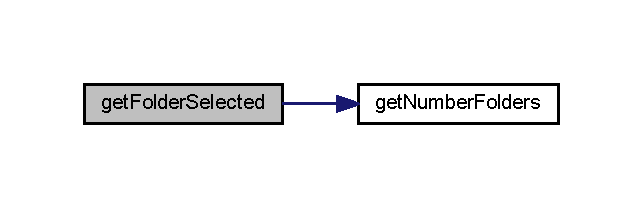
\includegraphics[width=308pt]{logic_8c_a4ea80b22f633b3030dec0db2269ada1d_cgraph}
\end{center}
\end{figure}


\hypertarget{logic_8c_a00fee6141a63232b663143211aacc392}{}\index{logic.\+c@{logic.\+c}!get\+Number\+Folders@{get\+Number\+Folders}}
\index{get\+Number\+Folders@{get\+Number\+Folders}!logic.\+c@{logic.\+c}}
\subsubsection[{get\+Number\+Folders}]{\setlength{\rightskip}{0pt plus 5cm}int get\+Number\+Folders (
\begin{DoxyParamCaption}
{}
\end{DoxyParamCaption}
)}\label{logic_8c_a00fee6141a63232b663143211aacc392}
Returns the number of folders 

Definition at line 338 of file logic.\+c.

\hypertarget{logic_8c_a551b12c420e086648c320df4fa034130}{}\index{logic.\+c@{logic.\+c}!get\+Path@{get\+Path}}
\index{get\+Path@{get\+Path}!logic.\+c@{logic.\+c}}
\subsubsection[{get\+Path}]{\setlength{\rightskip}{0pt plus 5cm}char$\ast$ get\+Path (
\begin{DoxyParamCaption}
{}
\end{DoxyParamCaption}
)}\label{logic_8c_a551b12c420e086648c320df4fa034130}
Returns the current path 

Definition at line 330 of file logic.\+c.

\hypertarget{logic_8c_a62436370dd4c3bd2452cef7f4fd7b7f0}{}\index{logic.\+c@{logic.\+c}!get\+Rename\+Flag@{get\+Rename\+Flag}}
\index{get\+Rename\+Flag@{get\+Rename\+Flag}!logic.\+c@{logic.\+c}}
\subsubsection[{get\+Rename\+Flag}]{\setlength{\rightskip}{0pt plus 5cm}int get\+Rename\+Flag (
\begin{DoxyParamCaption}
{}
\end{DoxyParamCaption}
)}\label{logic_8c_a62436370dd4c3bd2452cef7f4fd7b7f0}


Definition at line 144 of file logic.\+c.

\hypertarget{logic_8c_af25edb24b597453fb95c3c2080569bd5}{}\index{logic.\+c@{logic.\+c}!get\+Sub\+Folders@{get\+Sub\+Folders}}
\index{get\+Sub\+Folders@{get\+Sub\+Folders}!logic.\+c@{logic.\+c}}
\subsubsection[{get\+Sub\+Folders}]{\setlength{\rightskip}{0pt plus 5cm}int get\+Sub\+Folders (
\begin{DoxyParamCaption}
\item[{char $\ast$}]{foldername}
\end{DoxyParamCaption}
)}\label{logic_8c_af25edb24b597453fb95c3c2080569bd5}
Gets a folder subfolders, and stores them in a static array to be used later 

Definition at line 431 of file logic.\+c.



Here is the call graph for this function\+:\nopagebreak
\begin{figure}[H]
\begin{center}
\leavevmode
\includegraphics[width=262pt]{logic_8c_af25edb24b597453fb95c3c2080569bd5_cgraph}
\end{center}
\end{figure}


\hypertarget{logic_8c_a87d8b4ed67ed030ef2f6f3faeb7aa6df}{}\index{logic.\+c@{logic.\+c}!get\+Title@{get\+Title}}
\index{get\+Title@{get\+Title}!logic.\+c@{logic.\+c}}
\subsubsection[{get\+Title}]{\setlength{\rightskip}{0pt plus 5cm}char$\ast$ get\+Title (
\begin{DoxyParamCaption}
{}
\end{DoxyParamCaption}
)}\label{logic_8c_a87d8b4ed67ed030ef2f6f3faeb7aa6df}


Definition at line 193 of file logic.\+c.

\hypertarget{logic_8c_a283e5fd540509ad3e89cd63bb7f6e999}{}\index{logic.\+c@{logic.\+c}!get\+Turn\+Off\+Flag@{get\+Turn\+Off\+Flag}}
\index{get\+Turn\+Off\+Flag@{get\+Turn\+Off\+Flag}!logic.\+c@{logic.\+c}}
\subsubsection[{get\+Turn\+Off\+Flag}]{\setlength{\rightskip}{0pt plus 5cm}int get\+Turn\+Off\+Flag (
\begin{DoxyParamCaption}
{}
\end{DoxyParamCaption}
)}\label{logic_8c_a283e5fd540509ad3e89cd63bb7f6e999}
Returns turn off flag 

Definition at line 136 of file logic.\+c.

\hypertarget{logic_8c_a27d3ba5afb772cc36c9a432c28975ace}{}\index{logic.\+c@{logic.\+c}!init\+Buttons@{init\+Buttons}}
\index{init\+Buttons@{init\+Buttons}!logic.\+c@{logic.\+c}}
\subsubsection[{init\+Buttons}]{\setlength{\rightskip}{0pt plus 5cm}void init\+Buttons (
\begin{DoxyParamCaption}
{}
\end{DoxyParamCaption}
)}\label{logic_8c_a27d3ba5afb772cc36c9a432c28975ace}
Initiates interface buttons 

Definition at line 71 of file logic.\+c.



Here is the call graph for this function\+:\nopagebreak
\begin{figure}[H]
\begin{center}
\leavevmode
\includegraphics[width=238pt]{logic_8c_a27d3ba5afb772cc36c9a432c28975ace_cgraph}
\end{center}
\end{figure}


\hypertarget{logic_8c_a7400b316b1eb9244af06ab06f37757f8}{}\index{logic.\+c@{logic.\+c}!is\+Box@{is\+Box}}
\index{is\+Box@{is\+Box}!logic.\+c@{logic.\+c}}
\subsubsection[{is\+Box}]{\setlength{\rightskip}{0pt plus 5cm}int is\+Box (
\begin{DoxyParamCaption}
{}
\end{DoxyParamCaption}
)}\label{logic_8c_a7400b316b1eb9244af06ab06f37757f8}
Returns whether a box is active or not 

Definition at line 185 of file logic.\+c.

\hypertarget{logic_8c_a0e1eda02d10d0930fa24e87170c111ff}{}\index{logic.\+c@{logic.\+c}!is\+Box\+Confirmed@{is\+Box\+Confirmed}}
\index{is\+Box\+Confirmed@{is\+Box\+Confirmed}!logic.\+c@{logic.\+c}}
\subsubsection[{is\+Box\+Confirmed}]{\setlength{\rightskip}{0pt plus 5cm}int is\+Box\+Confirmed (
\begin{DoxyParamCaption}
{}
\end{DoxyParamCaption}
)}\label{logic_8c_a0e1eda02d10d0930fa24e87170c111ff}
Returns whether a box is confirmed or not 

Definition at line 149 of file logic.\+c.

\hypertarget{logic_8c_abfbb060a687a19a5ecb65b761bb153c0}{}\index{logic.\+c@{logic.\+c}!is\+File@{is\+File}}
\index{is\+File@{is\+File}!logic.\+c@{logic.\+c}}
\subsubsection[{is\+File}]{\setlength{\rightskip}{0pt plus 5cm}int is\+File (
\begin{DoxyParamCaption}
\item[{char $\ast$}]{path}
\end{DoxyParamCaption}
)}\label{logic_8c_abfbb060a687a19a5ecb65b761bb153c0}
Returns whether it is a file or a folder by path 

Definition at line 407 of file logic.\+c.

\hypertarget{logic_8c_a4b6ed6ccee9c7d03c7f1c93b51debcb7}{}\index{logic.\+c@{logic.\+c}!is\+File\+By\+Index@{is\+File\+By\+Index}}
\index{is\+File\+By\+Index@{is\+File\+By\+Index}!logic.\+c@{logic.\+c}}
\subsubsection[{is\+File\+By\+Index}]{\setlength{\rightskip}{0pt plus 5cm}int is\+File\+By\+Index (
\begin{DoxyParamCaption}
\item[{int}]{index}
\end{DoxyParamCaption}
)}\label{logic_8c_a4b6ed6ccee9c7d03c7f1c93b51debcb7}
Returns whether it is a file or a folder by index 

Definition at line 400 of file logic.\+c.

\hypertarget{logic_8c_a34121a3403c30a9dd71f71624aaaf0e7}{}\index{logic.\+c@{logic.\+c}!is\+Folder\+Selected@{is\+Folder\+Selected}}
\index{is\+Folder\+Selected@{is\+Folder\+Selected}!logic.\+c@{logic.\+c}}
\subsubsection[{is\+Folder\+Selected}]{\setlength{\rightskip}{0pt plus 5cm}int is\+Folder\+Selected (
\begin{DoxyParamCaption}
\item[{int}]{index}
\end{DoxyParamCaption}
)}\label{logic_8c_a34121a3403c30a9dd71f71624aaaf0e7}
Returns whether a certain folder is selected or not 

Definition at line 292 of file logic.\+c.

\hypertarget{logic_8c_a7b844fdb59d5c51e10bceedf336b6429}{}\index{logic.\+c@{logic.\+c}!is\+Output@{is\+Output}}
\index{is\+Output@{is\+Output}!logic.\+c@{logic.\+c}}
\subsubsection[{is\+Output}]{\setlength{\rightskip}{0pt plus 5cm}int is\+Output (
\begin{DoxyParamCaption}
{}
\end{DoxyParamCaption}
)}\label{logic_8c_a7b844fdb59d5c51e10bceedf336b6429}
Returns whether a box is out/input 

Definition at line 189 of file logic.\+c.

\hypertarget{logic_8c_a6ea97012f3e7cfbdac36a77b25046e9b}{}\index{logic.\+c@{logic.\+c}!move\+Back@{move\+Back}}
\index{move\+Back@{move\+Back}!logic.\+c@{logic.\+c}}
\subsubsection[{move\+Back}]{\setlength{\rightskip}{0pt plus 5cm}int move\+Back (
\begin{DoxyParamCaption}
{}
\end{DoxyParamCaption}
)}\label{logic_8c_a6ea97012f3e7cfbdac36a77b25046e9b}
Returns to initial folder by pressing backspace 

Definition at line 303 of file logic.\+c.



Here is the call graph for this function\+:\nopagebreak
\begin{figure}[H]
\begin{center}
\leavevmode
\includegraphics[width=350pt]{logic_8c_a6ea97012f3e7cfbdac36a77b25046e9b_cgraph}
\end{center}
\end{figure}


\hypertarget{logic_8c_a602ddea367dab1b4fec0e9f96abbcf0f}{}\index{logic.\+c@{logic.\+c}!navigate\+Down@{navigate\+Down}}
\index{navigate\+Down@{navigate\+Down}!logic.\+c@{logic.\+c}}
\subsubsection[{navigate\+Down}]{\setlength{\rightskip}{0pt plus 5cm}int navigate\+Down (
\begin{DoxyParamCaption}
{}
\end{DoxyParamCaption}
)}\label{logic_8c_a602ddea367dab1b4fec0e9f96abbcf0f}
Allows down arrow key navigation 

Definition at line 274 of file logic.\+c.



Here is the call graph for this function\+:\nopagebreak
\begin{figure}[H]
\begin{center}
\leavevmode
\includegraphics[width=350pt]{logic_8c_a602ddea367dab1b4fec0e9f96abbcf0f_cgraph}
\end{center}
\end{figure}


\hypertarget{logic_8c_ab8591ddf31e5c4ab28c07160e84ee893}{}\index{logic.\+c@{logic.\+c}!navigate\+Left@{navigate\+Left}}
\index{navigate\+Left@{navigate\+Left}!logic.\+c@{logic.\+c}}
\subsubsection[{navigate\+Left}]{\setlength{\rightskip}{0pt plus 5cm}int navigate\+Left (
\begin{DoxyParamCaption}
{}
\end{DoxyParamCaption}
)}\label{logic_8c_ab8591ddf31e5c4ab28c07160e84ee893}
Allows left arrow key navigation 

Definition at line 237 of file logic.\+c.



Here is the call graph for this function\+:\nopagebreak
\begin{figure}[H]
\begin{center}
\leavevmode
\includegraphics[width=350pt]{logic_8c_ab8591ddf31e5c4ab28c07160e84ee893_cgraph}
\end{center}
\end{figure}


\hypertarget{logic_8c_a87b6ad8fb397f0e72cbf79c99c3c3b25}{}\index{logic.\+c@{logic.\+c}!navigate\+Right@{navigate\+Right}}
\index{navigate\+Right@{navigate\+Right}!logic.\+c@{logic.\+c}}
\subsubsection[{navigate\+Right}]{\setlength{\rightskip}{0pt plus 5cm}int navigate\+Right (
\begin{DoxyParamCaption}
{}
\end{DoxyParamCaption}
)}\label{logic_8c_a87b6ad8fb397f0e72cbf79c99c3c3b25}
Allows right arrow key navigation 

Definition at line 249 of file logic.\+c.



Here is the call graph for this function\+:\nopagebreak
\begin{figure}[H]
\begin{center}
\leavevmode
\includegraphics[width=350pt]{logic_8c_a87b6ad8fb397f0e72cbf79c99c3c3b25_cgraph}
\end{center}
\end{figure}


\hypertarget{logic_8c_ade9da36feece104d5099779b77e0370d}{}\index{logic.\+c@{logic.\+c}!navigate\+Up@{navigate\+Up}}
\index{navigate\+Up@{navigate\+Up}!logic.\+c@{logic.\+c}}
\subsubsection[{navigate\+Up}]{\setlength{\rightskip}{0pt plus 5cm}int navigate\+Up (
\begin{DoxyParamCaption}
{}
\end{DoxyParamCaption}
)}\label{logic_8c_ade9da36feece104d5099779b77e0370d}
Allows up arrow key navigation 

Definition at line 262 of file logic.\+c.



Here is the call graph for this function\+:\nopagebreak
\begin{figure}[H]
\begin{center}
\leavevmode
\includegraphics[width=350pt]{logic_8c_ade9da36feece104d5099779b77e0370d_cgraph}
\end{center}
\end{figure}


\hypertarget{logic_8c_a913ad8296c70b807df4fbf6302f8072a}{}\index{logic.\+c@{logic.\+c}!open\+Folder@{open\+Folder}}
\index{open\+Folder@{open\+Folder}!logic.\+c@{logic.\+c}}
\subsubsection[{open\+Folder}]{\setlength{\rightskip}{0pt plus 5cm}void open\+Folder (
\begin{DoxyParamCaption}
\item[{int}]{index}
\end{DoxyParamCaption}
)}\label{logic_8c_a913ad8296c70b807df4fbf6302f8072a}
Opens folder with a certain index 

Definition at line 155 of file logic.\+c.



Here is the call graph for this function\+:\nopagebreak
\begin{figure}[H]
\begin{center}
\leavevmode
\includegraphics[width=350pt]{logic_8c_a913ad8296c70b807df4fbf6302f8072a_cgraph}
\end{center}
\end{figure}


\hypertarget{logic_8c_a317bd44d55f4edc8580bbdbdc8a5f506}{}\index{logic.\+c@{logic.\+c}!open\+Folder\+By\+Enter@{open\+Folder\+By\+Enter}}
\index{open\+Folder\+By\+Enter@{open\+Folder\+By\+Enter}!logic.\+c@{logic.\+c}}
\subsubsection[{open\+Folder\+By\+Enter}]{\setlength{\rightskip}{0pt plus 5cm}int open\+Folder\+By\+Enter (
\begin{DoxyParamCaption}
{}
\end{DoxyParamCaption}
)}\label{logic_8c_a317bd44d55f4edc8580bbdbdc8a5f506}
Allows opening a folder by pressing Enter 

Definition at line 297 of file logic.\+c.



Here is the call graph for this function\+:\nopagebreak
\begin{figure}[H]
\begin{center}
\leavevmode
\includegraphics[width=350pt]{logic_8c_a317bd44d55f4edc8580bbdbdc8a5f506_cgraph}
\end{center}
\end{figure}


\hypertarget{logic_8c_a1e48323b0a3fdd311f7cd1988532ace8}{}\index{logic.\+c@{logic.\+c}!rename\+Folder@{rename\+Folder}}
\index{rename\+Folder@{rename\+Folder}!logic.\+c@{logic.\+c}}
\subsubsection[{rename\+Folder}]{\setlength{\rightskip}{0pt plus 5cm}void rename\+Folder (
\begin{DoxyParamCaption}
\item[{int}]{index}
\end{DoxyParamCaption}
)}\label{logic_8c_a1e48323b0a3fdd311f7cd1988532ace8}
Receives an index of a folder to rename and uses the text from the input box to do so 
\begin{DoxyParams}{Parameters}
{\em index} & \\
\hline
\end{DoxyParams}


Definition at line 212 of file logic.\+c.



Here is the call graph for this function\+:\nopagebreak
\begin{figure}[H]
\begin{center}
\leavevmode
\includegraphics[width=350pt]{logic_8c_a1e48323b0a3fdd311f7cd1988532ace8_cgraph}
\end{center}
\end{figure}


\hypertarget{logic_8c_a20a866a30fdbb32fc9bfc74dacd0b89c}{}\index{logic.\+c@{logic.\+c}!set\+Delete\+Flag@{set\+Delete\+Flag}}
\index{set\+Delete\+Flag@{set\+Delete\+Flag}!logic.\+c@{logic.\+c}}
\subsubsection[{set\+Delete\+Flag}]{\setlength{\rightskip}{0pt plus 5cm}void set\+Delete\+Flag (
\begin{DoxyParamCaption}
{}
\end{DoxyParamCaption}
)}\label{logic_8c_a20a866a30fdbb32fc9bfc74dacd0b89c}
Activates delete flag 

Definition at line 128 of file logic.\+c.

\hypertarget{logic_8c_a3b3c14dae824723e0e1b4720a370b3e6}{}\index{logic.\+c@{logic.\+c}!set\+Folder\+Coords@{set\+Folder\+Coords}}
\index{set\+Folder\+Coords@{set\+Folder\+Coords}!logic.\+c@{logic.\+c}}
\subsubsection[{set\+Folder\+Coords}]{\setlength{\rightskip}{0pt plus 5cm}void set\+Folder\+Coords (
\begin{DoxyParamCaption}
\item[{int}]{index, }
\item[{int}]{in\+X, }
\item[{int}]{in\+Y}
\end{DoxyParamCaption}
)}\label{logic_8c_a3b3c14dae824723e0e1b4720a370b3e6}
Sets folder coords 

Definition at line 319 of file logic.\+c.

\hypertarget{logic_8c_a6673774c3b7ef292567a5637f47a9579}{}\index{logic.\+c@{logic.\+c}!set\+Rename\+Flag@{set\+Rename\+Flag}}
\index{set\+Rename\+Flag@{set\+Rename\+Flag}!logic.\+c@{logic.\+c}}
\subsubsection[{set\+Rename\+Flag}]{\setlength{\rightskip}{0pt plus 5cm}void set\+Rename\+Flag (
\begin{DoxyParamCaption}
{}
\end{DoxyParamCaption}
)}\label{logic_8c_a6673774c3b7ef292567a5637f47a9579}
Sets rename flag to true 

Definition at line 140 of file logic.\+c.

\hypertarget{logic_8c_aa9f20f8c541306d3b93879d0a6d497e8}{}\index{logic.\+c@{logic.\+c}!toggle\+Selected@{toggle\+Selected}}
\index{toggle\+Selected@{toggle\+Selected}!logic.\+c@{logic.\+c}}
\subsubsection[{toggle\+Selected}]{\setlength{\rightskip}{0pt plus 5cm}void toggle\+Selected (
\begin{DoxyParamCaption}
\item[{int}]{index}
\end{DoxyParamCaption}
)}\label{logic_8c_aa9f20f8c541306d3b93879d0a6d497e8}
Selects/\+Unselects a certain folder 

Definition at line 324 of file logic.\+c.

\hypertarget{logic_8c_a5b0080e32e3cb075b00c7184ce3f5ad0}{}\index{logic.\+c@{logic.\+c}!update\+Path@{update\+Path}}
\index{update\+Path@{update\+Path}!logic.\+c@{logic.\+c}}
\subsubsection[{update\+Path}]{\setlength{\rightskip}{0pt plus 5cm}void update\+Path (
\begin{DoxyParamCaption}
\item[{char $\ast$}]{foldername}
\end{DoxyParamCaption}
)}\label{logic_8c_a5b0080e32e3cb075b00c7184ce3f5ad0}
Given a foldername this function updates the current path, if file doesn\textquotesingle{}t 
\begin{DoxyParams}{Parameters}
{\em foldername} & \\
\hline
\end{DoxyParams}


Definition at line 416 of file logic.\+c.

\hypertarget{logic_8c_a501609335890024a00bc939c19538b0f}{}\index{logic.\+c@{logic.\+c}!update\+Text\+Box@{update\+Text\+Box}}
\index{update\+Text\+Box@{update\+Text\+Box}!logic.\+c@{logic.\+c}}
\subsubsection[{update\+Text\+Box}]{\setlength{\rightskip}{0pt plus 5cm}void update\+Text\+Box (
\begin{DoxyParamCaption}
\item[{unsigned long}]{input}
\end{DoxyParamCaption}
)}\label{logic_8c_a501609335890024a00bc939c19538b0f}


Definition at line 390 of file logic.\+c.



Here is the call graph for this function\+:\nopagebreak
\begin{figure}[H]
\begin{center}
\leavevmode
\includegraphics[width=294pt]{logic_8c_a501609335890024a00bc939c19538b0f_cgraph}
\end{center}
\end{figure}



\hypertarget{logic_8h}{}\section{logic.\+h File Reference}
\label{logic_8h}\index{logic.\+h@{logic.\+h}}
{\ttfamily \#include \char`\"{}mouse.\+h\char`\"{}}\\*
{\ttfamily \#include $<$sys/types.\+h$>$}\\*
{\ttfamily \#include $<$dirent.\+h$>$}\\*
{\ttfamily \#include $<$stdlib.\+h$>$}\\*
{\ttfamily \#include $<$unistd.\+h$>$}\\*
{\ttfamily \#include $<$sys/stat.\+h$>$}\\*
\subsection*{Classes}
\begin{DoxyCompactItemize}
\item 
struct \hyperlink{struct_buttons}{Buttons}
\item 
struct \hyperlink{struct_directories}{Directories}
\item 
struct \hyperlink{structioboxes}{ioboxes}
\end{DoxyCompactItemize}
\subsection*{Typedefs}
\begin{DoxyCompactItemize}
\item 
typedef struct \hyperlink{struct_buttons}{Buttons} \hyperlink{logic_8h_a8dd5b76d2972cdce6fd4f1c7d8e175c5}{Button}
\item 
typedef struct \hyperlink{struct_directories}{Directories} \hyperlink{logic_8h_ad5e554666c5d1a199d39416c639f97f8}{Directory}
\item 
typedef struct \hyperlink{structioboxes}{ioboxes} \hyperlink{logic_8h_a33a5fb9138c64886656bb3badd773151}{iobox}
\end{DoxyCompactItemize}
\subsection*{Functions}
\begin{DoxyCompactItemize}
\item 
int \hyperlink{logic_8h_a0a12179d687ca2d67e72e78268f7cc2c}{collision} (\hyperlink{structmouse__state}{mouse\+\_\+state} mouse, \hyperlink{logic_8h_a8dd5b76d2972cdce6fd4f1c7d8e175c5}{Button} a)
\item 
int \hyperlink{logic_8h_aa39071f67e32c2002f72ce59c1e6fa11}{check\+\_\+mouse\+\_\+click} (\hyperlink{structmouse__state}{mouse\+\_\+state} \hyperlink{state_8h_a39d9a371f9aef2042923a96e2f855d5e}{current\+\_\+mouse\+\_\+state})
\item 
void \hyperlink{logic_8h_a27d3ba5afb772cc36c9a432c28975ace}{init\+Buttons} ()
\item 
int \hyperlink{logic_8h_ab16ca2694321ab91f2f0a0b332c0df58}{check\+\_\+mouse\+\_\+double\+\_\+click} (\hyperlink{structmouse__state}{mouse\+\_\+state} \hyperlink{state_8h_a39d9a371f9aef2042923a96e2f855d5e}{current\+\_\+mouse\+\_\+state})
\item 
int \hyperlink{logic_8h_ac4ac4a95ff10cf3256c2a36d0e90d45e}{check\+\_\+delete\+\_\+files} ()
\item 
void \hyperlink{logic_8h_a20a866a30fdbb32fc9bfc74dacd0b89c}{set\+Delete\+Flag} ()
\item 
int \hyperlink{logic_8h_aaa9525bb143ec0e36c7b6eda42881715}{get\+Delete\+Flag} ()
\item 
void \hyperlink{logic_8h_a6673774c3b7ef292567a5637f47a9579}{set\+Rename\+Flag} ()
\item 
void \hyperlink{logic_8h_a1e48323b0a3fdd311f7cd1988532ace8}{rename\+Folder} (int index)
\item 
int \hyperlink{logic_8h_a62436370dd4c3bd2452cef7f4fd7b7f0}{get\+Rename\+Flag} ()
\item 
int \hyperlink{logic_8h_a283e5fd540509ad3e89cd63bb7f6e999}{get\+Turn\+Off\+Flag} ()
\item 
int \hyperlink{logic_8h_a0e1eda02d10d0930fa24e87170c111ff}{is\+Box\+Confirmed} ()
\item 
void \hyperlink{logic_8h_a913ad8296c70b807df4fbf6302f8072a}{open\+Folder} (int index)
\item 
void \hyperlink{logic_8h_a0d8e78acd24989789082f4306f903596}{disable\+Box} ()
\item 
void \hyperlink{logic_8h_a017ced8b7330e5d2522c9718de024750}{enable\+Box} (int type, char $\ast$title, char $\ast$text)
\item 
char $\ast$ \hyperlink{logic_8h_a158bfa83c4b1dd186a3a89151b687e01}{get\+Box\+Text} ()
\item 
int \hyperlink{logic_8h_a7400b316b1eb9244af06ab06f37757f8}{is\+Box} ()
\item 
int \hyperlink{logic_8h_a7b844fdb59d5c51e10bceedf336b6429}{is\+Output} ()
\item 
void \hyperlink{logic_8h_a530fba246396179676ecb402fb2d2e4a}{delete\+Folder} (int index)
\item 
int \hyperlink{logic_8h_ab8591ddf31e5c4ab28c07160e84ee893}{navigate\+Left} ()
\item 
int \hyperlink{logic_8h_a87b6ad8fb397f0e72cbf79c99c3c3b25}{navigate\+Right} ()
\item 
int \hyperlink{logic_8h_ade9da36feece104d5099779b77e0370d}{navigate\+Up} ()
\item 
int \hyperlink{logic_8h_a602ddea367dab1b4fec0e9f96abbcf0f}{navigate\+Down} ()
\item 
char $\ast$ \hyperlink{logic_8h_a31ba4de847c8b9762dfe9fdbb08ef4f1}{get\+Folder\+Name} (int index)
\item 
int \hyperlink{logic_8h_a34121a3403c30a9dd71f71624aaaf0e7}{is\+Folder\+Selected} (int index)
\item 
int \hyperlink{logic_8h_a317bd44d55f4edc8580bbdbdc8a5f506}{open\+Folder\+By\+Enter} ()
\item 
int \hyperlink{logic_8h_a6ea97012f3e7cfbdac36a77b25046e9b}{move\+Back} ()
\item 
int \hyperlink{logic_8h_a4ea80b22f633b3030dec0db2269ada1d}{get\+Folder\+Selected} ()
\item 
void \hyperlink{logic_8h_a3b3c14dae824723e0e1b4720a370b3e6}{set\+Folder\+Coords} (int index, int in\+X, int in\+Y)
\item 
void \hyperlink{logic_8h_aa9f20f8c541306d3b93879d0a6d497e8}{toggle\+Selected} (int index)
\item 
char $\ast$ \hyperlink{logic_8h_a551b12c420e086648c320df4fa034130}{get\+Path} ()
\item 
\hyperlink{logic_8h_ad5e554666c5d1a199d39416c639f97f8}{Directory} $\ast$ \hyperlink{logic_8h_a4b7468f1ca81496cf0ee00452194e81f}{get\+Directories} ()
\item 
int \hyperlink{logic_8h_a00fee6141a63232b663143211aacc392}{get\+Number\+Folders} ()
\item 
int \hyperlink{logic_8h_a65b0f047568e3d106306bd405b5be72b}{get\+Folder\+By\+Coords} (int x, int y)
\item 
int \hyperlink{logic_8h_a4b6ed6ccee9c7d03c7f1c93b51debcb7}{is\+File\+By\+Index} (int index)
\item 
int \hyperlink{logic_8h_abfbb060a687a19a5ecb65b761bb153c0}{is\+File} (char $\ast$path)
\item 
void \hyperlink{logic_8h_a5b0080e32e3cb075b00c7184ce3f5ad0}{update\+Path} (char $\ast$foldername)
\item 
int \hyperlink{logic_8h_af25edb24b597453fb95c3c2080569bd5}{get\+Sub\+Folders} (char $\ast$foldername)
\end{DoxyCompactItemize}
\subsection*{Variables}
\begin{DoxyCompactItemize}
\item 
\hyperlink{logic_8h_ad5e554666c5d1a199d39416c639f97f8}{Directory} \hyperlink{logic_8h_a3373e62de40b1409be028a7cbe926cbd}{current\+Folders} \mbox{[}100\mbox{]}
\end{DoxyCompactItemize}


\subsection{Typedef Documentation}
\hypertarget{logic_8h_a8dd5b76d2972cdce6fd4f1c7d8e175c5}{}\index{logic.\+h@{logic.\+h}!Button@{Button}}
\index{Button@{Button}!logic.\+h@{logic.\+h}}
\subsubsection[{Button}]{\setlength{\rightskip}{0pt plus 5cm}typedef struct {\bf Buttons}  {\bf Button}}\label{logic_8h_a8dd5b76d2972cdce6fd4f1c7d8e175c5}
Struct to handle buttons of the interface \hypertarget{logic_8h_ad5e554666c5d1a199d39416c639f97f8}{}\index{logic.\+h@{logic.\+h}!Directory@{Directory}}
\index{Directory@{Directory}!logic.\+h@{logic.\+h}}
\subsubsection[{Directory}]{\setlength{\rightskip}{0pt plus 5cm}typedef struct {\bf Directories}  {\bf Directory}}\label{logic_8h_ad5e554666c5d1a199d39416c639f97f8}
Struct to handle directories \hypertarget{logic_8h_a33a5fb9138c64886656bb3badd773151}{}\index{logic.\+h@{logic.\+h}!iobox@{iobox}}
\index{iobox@{iobox}!logic.\+h@{logic.\+h}}
\subsubsection[{iobox}]{\setlength{\rightskip}{0pt plus 5cm}typedef struct {\bf ioboxes}  {\bf iobox}}\label{logic_8h_a33a5fb9138c64886656bb3badd773151}
Struct to handle I/\+O boxes 

\subsection{Function Documentation}
\hypertarget{logic_8h_ac4ac4a95ff10cf3256c2a36d0e90d45e}{}\index{logic.\+h@{logic.\+h}!check\+\_\+delete\+\_\+files@{check\+\_\+delete\+\_\+files}}
\index{check\+\_\+delete\+\_\+files@{check\+\_\+delete\+\_\+files}!logic.\+h@{logic.\+h}}
\subsubsection[{check\+\_\+delete\+\_\+files}]{\setlength{\rightskip}{0pt plus 5cm}int check\+\_\+delete\+\_\+files (
\begin{DoxyParamCaption}
{}
\end{DoxyParamCaption}
)}\label{logic_8h_ac4ac4a95ff10cf3256c2a36d0e90d45e}
Deletes selected folder/file 

Definition at line 112 of file logic.\+c.



Here is the call graph for this function\+:\nopagebreak
\begin{figure}[H]
\begin{center}
\leavevmode
\includegraphics[width=350pt]{logic_8h_ac4ac4a95ff10cf3256c2a36d0e90d45e_cgraph}
\end{center}
\end{figure}


\hypertarget{logic_8h_aa39071f67e32c2002f72ce59c1e6fa11}{}\index{logic.\+h@{logic.\+h}!check\+\_\+mouse\+\_\+click@{check\+\_\+mouse\+\_\+click}}
\index{check\+\_\+mouse\+\_\+click@{check\+\_\+mouse\+\_\+click}!logic.\+h@{logic.\+h}}
\subsubsection[{check\+\_\+mouse\+\_\+click}]{\setlength{\rightskip}{0pt plus 5cm}int check\+\_\+mouse\+\_\+click (
\begin{DoxyParamCaption}
\item[{{\bf mouse\+\_\+state}}]{current\+\_\+mouse\+\_\+state}
\end{DoxyParamCaption}
)}\label{logic_8h_aa39071f67e32c2002f72ce59c1e6fa11}
Does verifications when the mouse is clicked once 
\begin{DoxyParams}{Parameters}
{\em current\+\_\+mouse\+\_\+state} & \\
\hline
\end{DoxyParams}
\begin{DoxyReturn}{Returns}

\end{DoxyReturn}


Definition at line 19 of file logic.\+c.



Here is the call graph for this function\+:\nopagebreak
\begin{figure}[H]
\begin{center}
\leavevmode
\includegraphics[width=320pt]{logic_8h_aa39071f67e32c2002f72ce59c1e6fa11_cgraph}
\end{center}
\end{figure}


\hypertarget{logic_8h_ab16ca2694321ab91f2f0a0b332c0df58}{}\index{logic.\+h@{logic.\+h}!check\+\_\+mouse\+\_\+double\+\_\+click@{check\+\_\+mouse\+\_\+double\+\_\+click}}
\index{check\+\_\+mouse\+\_\+double\+\_\+click@{check\+\_\+mouse\+\_\+double\+\_\+click}!logic.\+h@{logic.\+h}}
\subsubsection[{check\+\_\+mouse\+\_\+double\+\_\+click}]{\setlength{\rightskip}{0pt plus 5cm}int check\+\_\+mouse\+\_\+double\+\_\+click (
\begin{DoxyParamCaption}
\item[{{\bf mouse\+\_\+state}}]{current\+\_\+mouse\+\_\+state}
\end{DoxyParamCaption}
)}\label{logic_8h_ab16ca2694321ab91f2f0a0b332c0df58}
Does verifications when the mouse is clicked twice in less than 0.\+25 seconds (double click) 
\begin{DoxyParams}{Parameters}
{\em current\+\_\+mouse\+\_\+state} & \\
\hline
\end{DoxyParams}
\begin{DoxyReturn}{Returns}

\end{DoxyReturn}


Definition at line 83 of file logic.\+c.



Here is the call graph for this function\+:\nopagebreak
\begin{figure}[H]
\begin{center}
\leavevmode
\includegraphics[width=350pt]{logic_8h_ab16ca2694321ab91f2f0a0b332c0df58_cgraph}
\end{center}
\end{figure}


\hypertarget{logic_8h_a0a12179d687ca2d67e72e78268f7cc2c}{}\index{logic.\+h@{logic.\+h}!collision@{collision}}
\index{collision@{collision}!logic.\+h@{logic.\+h}}
\subsubsection[{collision}]{\setlength{\rightskip}{0pt plus 5cm}int collision (
\begin{DoxyParamCaption}
\item[{{\bf mouse\+\_\+state}}]{mouse, }
\item[{{\bf Button}}]{a}
\end{DoxyParamCaption}
)}\label{logic_8h_a0a12179d687ca2d67e72e78268f7cc2c}
Handles mouse collisions 
\begin{DoxyParams}{Parameters}
{\em mouse} & \\
\hline
{\em a} & \\
\hline
\end{DoxyParams}
\begin{DoxyReturn}{Returns}

\end{DoxyReturn}


Definition at line 8 of file logic.\+c.

\hypertarget{logic_8h_a530fba246396179676ecb402fb2d2e4a}{}\index{logic.\+h@{logic.\+h}!delete\+Folder@{delete\+Folder}}
\index{delete\+Folder@{delete\+Folder}!logic.\+h@{logic.\+h}}
\subsubsection[{delete\+Folder}]{\setlength{\rightskip}{0pt plus 5cm}void delete\+Folder (
\begin{DoxyParamCaption}
\item[{int}]{index}
\end{DoxyParamCaption}
)}\label{logic_8h_a530fba246396179676ecb402fb2d2e4a}
Deletes a folder with a certain index 

Definition at line 198 of file logic.\+c.



Here is the call graph for this function\+:\nopagebreak
\begin{figure}[H]
\begin{center}
\leavevmode
\includegraphics[width=350pt]{logic_8h_a530fba246396179676ecb402fb2d2e4a_cgraph}
\end{center}
\end{figure}


\hypertarget{logic_8h_a0d8e78acd24989789082f4306f903596}{}\index{logic.\+h@{logic.\+h}!disable\+Box@{disable\+Box}}
\index{disable\+Box@{disable\+Box}!logic.\+h@{logic.\+h}}
\subsubsection[{disable\+Box}]{\setlength{\rightskip}{0pt plus 5cm}void disable\+Box (
\begin{DoxyParamCaption}
{}
\end{DoxyParamCaption}
)}\label{logic_8h_a0d8e78acd24989789082f4306f903596}
Disables box 

Definition at line 160 of file logic.\+c.

\hypertarget{logic_8h_a017ced8b7330e5d2522c9718de024750}{}\index{logic.\+h@{logic.\+h}!enable\+Box@{enable\+Box}}
\index{enable\+Box@{enable\+Box}!logic.\+h@{logic.\+h}}
\subsubsection[{enable\+Box}]{\setlength{\rightskip}{0pt plus 5cm}void enable\+Box (
\begin{DoxyParamCaption}
\item[{int}]{type, }
\item[{char $\ast$}]{title, }
\item[{char $\ast$}]{text}
\end{DoxyParamCaption}
)}\label{logic_8h_a017ced8b7330e5d2522c9718de024750}
Enables box 

Definition at line 167 of file logic.\+c.

\hypertarget{logic_8h_a158bfa83c4b1dd186a3a89151b687e01}{}\index{logic.\+h@{logic.\+h}!get\+Box\+Text@{get\+Box\+Text}}
\index{get\+Box\+Text@{get\+Box\+Text}!logic.\+h@{logic.\+h}}
\subsubsection[{get\+Box\+Text}]{\setlength{\rightskip}{0pt plus 5cm}char$\ast$ get\+Box\+Text (
\begin{DoxyParamCaption}
{}
\end{DoxyParamCaption}
)}\label{logic_8h_a158bfa83c4b1dd186a3a89151b687e01}
Gets a box input 

Definition at line 181 of file logic.\+c.

\hypertarget{logic_8h_aaa9525bb143ec0e36c7b6eda42881715}{}\index{logic.\+h@{logic.\+h}!get\+Delete\+Flag@{get\+Delete\+Flag}}
\index{get\+Delete\+Flag@{get\+Delete\+Flag}!logic.\+h@{logic.\+h}}
\subsubsection[{get\+Delete\+Flag}]{\setlength{\rightskip}{0pt plus 5cm}int get\+Delete\+Flag (
\begin{DoxyParamCaption}
{}
\end{DoxyParamCaption}
)}\label{logic_8h_aaa9525bb143ec0e36c7b6eda42881715}
Returns delete flag 

Definition at line 132 of file logic.\+c.

\hypertarget{logic_8h_a4b7468f1ca81496cf0ee00452194e81f}{}\index{logic.\+h@{logic.\+h}!get\+Directories@{get\+Directories}}
\index{get\+Directories@{get\+Directories}!logic.\+h@{logic.\+h}}
\subsubsection[{get\+Directories}]{\setlength{\rightskip}{0pt plus 5cm}{\bf Directory}$\ast$ get\+Directories (
\begin{DoxyParamCaption}
{}
\end{DoxyParamCaption}
)}\label{logic_8h_a4b7468f1ca81496cf0ee00452194e81f}
Returns current folders of the current directory 

Definition at line 334 of file logic.\+c.

\hypertarget{logic_8h_a65b0f047568e3d106306bd405b5be72b}{}\index{logic.\+h@{logic.\+h}!get\+Folder\+By\+Coords@{get\+Folder\+By\+Coords}}
\index{get\+Folder\+By\+Coords@{get\+Folder\+By\+Coords}!logic.\+h@{logic.\+h}}
\subsubsection[{get\+Folder\+By\+Coords}]{\setlength{\rightskip}{0pt plus 5cm}int get\+Folder\+By\+Coords (
\begin{DoxyParamCaption}
\item[{int}]{x, }
\item[{int}]{y}
\end{DoxyParamCaption}
)}\label{logic_8h_a65b0f047568e3d106306bd405b5be72b}
Gets folder index by coordinates 

Definition at line 343 of file logic.\+c.

\hypertarget{logic_8h_a31ba4de847c8b9762dfe9fdbb08ef4f1}{}\index{logic.\+h@{logic.\+h}!get\+Folder\+Name@{get\+Folder\+Name}}
\index{get\+Folder\+Name@{get\+Folder\+Name}!logic.\+h@{logic.\+h}}
\subsubsection[{get\+Folder\+Name}]{\setlength{\rightskip}{0pt plus 5cm}char$\ast$ get\+Folder\+Name (
\begin{DoxyParamCaption}
\item[{int}]{index}
\end{DoxyParamCaption}
)}\label{logic_8h_a31ba4de847c8b9762dfe9fdbb08ef4f1}
Returns a folder\textquotesingle{}s name with a certain index 

Definition at line 288 of file logic.\+c.

\hypertarget{logic_8h_a4ea80b22f633b3030dec0db2269ada1d}{}\index{logic.\+h@{logic.\+h}!get\+Folder\+Selected@{get\+Folder\+Selected}}
\index{get\+Folder\+Selected@{get\+Folder\+Selected}!logic.\+h@{logic.\+h}}
\subsubsection[{get\+Folder\+Selected}]{\setlength{\rightskip}{0pt plus 5cm}int get\+Folder\+Selected (
\begin{DoxyParamCaption}
{}
\end{DoxyParamCaption}
)}\label{logic_8h_a4ea80b22f633b3030dec0db2269ada1d}
Returns index of the folder currently selected 

Definition at line 308 of file logic.\+c.



Here is the call graph for this function\+:\nopagebreak
\begin{figure}[H]
\begin{center}
\leavevmode
\includegraphics[width=308pt]{logic_8h_a4ea80b22f633b3030dec0db2269ada1d_cgraph}
\end{center}
\end{figure}


\hypertarget{logic_8h_a00fee6141a63232b663143211aacc392}{}\index{logic.\+h@{logic.\+h}!get\+Number\+Folders@{get\+Number\+Folders}}
\index{get\+Number\+Folders@{get\+Number\+Folders}!logic.\+h@{logic.\+h}}
\subsubsection[{get\+Number\+Folders}]{\setlength{\rightskip}{0pt plus 5cm}int get\+Number\+Folders (
\begin{DoxyParamCaption}
{}
\end{DoxyParamCaption}
)}\label{logic_8h_a00fee6141a63232b663143211aacc392}
Returns the number of folders 

Definition at line 338 of file logic.\+c.

\hypertarget{logic_8h_a551b12c420e086648c320df4fa034130}{}\index{logic.\+h@{logic.\+h}!get\+Path@{get\+Path}}
\index{get\+Path@{get\+Path}!logic.\+h@{logic.\+h}}
\subsubsection[{get\+Path}]{\setlength{\rightskip}{0pt plus 5cm}char$\ast$ get\+Path (
\begin{DoxyParamCaption}
{}
\end{DoxyParamCaption}
)}\label{logic_8h_a551b12c420e086648c320df4fa034130}
Returns the current path 

Definition at line 330 of file logic.\+c.

\hypertarget{logic_8h_a62436370dd4c3bd2452cef7f4fd7b7f0}{}\index{logic.\+h@{logic.\+h}!get\+Rename\+Flag@{get\+Rename\+Flag}}
\index{get\+Rename\+Flag@{get\+Rename\+Flag}!logic.\+h@{logic.\+h}}
\subsubsection[{get\+Rename\+Flag}]{\setlength{\rightskip}{0pt plus 5cm}int get\+Rename\+Flag (
\begin{DoxyParamCaption}
{}
\end{DoxyParamCaption}
)}\label{logic_8h_a62436370dd4c3bd2452cef7f4fd7b7f0}


Definition at line 144 of file logic.\+c.

\hypertarget{logic_8h_af25edb24b597453fb95c3c2080569bd5}{}\index{logic.\+h@{logic.\+h}!get\+Sub\+Folders@{get\+Sub\+Folders}}
\index{get\+Sub\+Folders@{get\+Sub\+Folders}!logic.\+h@{logic.\+h}}
\subsubsection[{get\+Sub\+Folders}]{\setlength{\rightskip}{0pt plus 5cm}int get\+Sub\+Folders (
\begin{DoxyParamCaption}
\item[{char $\ast$}]{foldername}
\end{DoxyParamCaption}
)}\label{logic_8h_af25edb24b597453fb95c3c2080569bd5}
Gets a folder subfolders, and stores them in a static array to be used later 

Definition at line 431 of file logic.\+c.



Here is the call graph for this function\+:\nopagebreak
\begin{figure}[H]
\begin{center}
\leavevmode
\includegraphics[width=262pt]{logic_8h_af25edb24b597453fb95c3c2080569bd5_cgraph}
\end{center}
\end{figure}


\hypertarget{logic_8h_a283e5fd540509ad3e89cd63bb7f6e999}{}\index{logic.\+h@{logic.\+h}!get\+Turn\+Off\+Flag@{get\+Turn\+Off\+Flag}}
\index{get\+Turn\+Off\+Flag@{get\+Turn\+Off\+Flag}!logic.\+h@{logic.\+h}}
\subsubsection[{get\+Turn\+Off\+Flag}]{\setlength{\rightskip}{0pt plus 5cm}int get\+Turn\+Off\+Flag (
\begin{DoxyParamCaption}
{}
\end{DoxyParamCaption}
)}\label{logic_8h_a283e5fd540509ad3e89cd63bb7f6e999}
Returns turn off flag 

Definition at line 136 of file logic.\+c.

\hypertarget{logic_8h_a27d3ba5afb772cc36c9a432c28975ace}{}\index{logic.\+h@{logic.\+h}!init\+Buttons@{init\+Buttons}}
\index{init\+Buttons@{init\+Buttons}!logic.\+h@{logic.\+h}}
\subsubsection[{init\+Buttons}]{\setlength{\rightskip}{0pt plus 5cm}void init\+Buttons (
\begin{DoxyParamCaption}
{}
\end{DoxyParamCaption}
)}\label{logic_8h_a27d3ba5afb772cc36c9a432c28975ace}
Initiates interface buttons 

Definition at line 71 of file logic.\+c.



Here is the call graph for this function\+:\nopagebreak
\begin{figure}[H]
\begin{center}
\leavevmode
\includegraphics[width=238pt]{logic_8h_a27d3ba5afb772cc36c9a432c28975ace_cgraph}
\end{center}
\end{figure}


\hypertarget{logic_8h_a7400b316b1eb9244af06ab06f37757f8}{}\index{logic.\+h@{logic.\+h}!is\+Box@{is\+Box}}
\index{is\+Box@{is\+Box}!logic.\+h@{logic.\+h}}
\subsubsection[{is\+Box}]{\setlength{\rightskip}{0pt plus 5cm}int is\+Box (
\begin{DoxyParamCaption}
{}
\end{DoxyParamCaption}
)}\label{logic_8h_a7400b316b1eb9244af06ab06f37757f8}
Returns whether a box is active or not 

Definition at line 185 of file logic.\+c.

\hypertarget{logic_8h_a0e1eda02d10d0930fa24e87170c111ff}{}\index{logic.\+h@{logic.\+h}!is\+Box\+Confirmed@{is\+Box\+Confirmed}}
\index{is\+Box\+Confirmed@{is\+Box\+Confirmed}!logic.\+h@{logic.\+h}}
\subsubsection[{is\+Box\+Confirmed}]{\setlength{\rightskip}{0pt plus 5cm}int is\+Box\+Confirmed (
\begin{DoxyParamCaption}
{}
\end{DoxyParamCaption}
)}\label{logic_8h_a0e1eda02d10d0930fa24e87170c111ff}
Returns whether a box is confirmed or not 

Definition at line 149 of file logic.\+c.

\hypertarget{logic_8h_abfbb060a687a19a5ecb65b761bb153c0}{}\index{logic.\+h@{logic.\+h}!is\+File@{is\+File}}
\index{is\+File@{is\+File}!logic.\+h@{logic.\+h}}
\subsubsection[{is\+File}]{\setlength{\rightskip}{0pt plus 5cm}int is\+File (
\begin{DoxyParamCaption}
\item[{char $\ast$}]{path}
\end{DoxyParamCaption}
)}\label{logic_8h_abfbb060a687a19a5ecb65b761bb153c0}
Returns whether it is a file or a folder by path 

Definition at line 407 of file logic.\+c.

\hypertarget{logic_8h_a4b6ed6ccee9c7d03c7f1c93b51debcb7}{}\index{logic.\+h@{logic.\+h}!is\+File\+By\+Index@{is\+File\+By\+Index}}
\index{is\+File\+By\+Index@{is\+File\+By\+Index}!logic.\+h@{logic.\+h}}
\subsubsection[{is\+File\+By\+Index}]{\setlength{\rightskip}{0pt plus 5cm}int is\+File\+By\+Index (
\begin{DoxyParamCaption}
\item[{int}]{index}
\end{DoxyParamCaption}
)}\label{logic_8h_a4b6ed6ccee9c7d03c7f1c93b51debcb7}
Returns whether it is a file or a folder by index 

Definition at line 400 of file logic.\+c.

\hypertarget{logic_8h_a34121a3403c30a9dd71f71624aaaf0e7}{}\index{logic.\+h@{logic.\+h}!is\+Folder\+Selected@{is\+Folder\+Selected}}
\index{is\+Folder\+Selected@{is\+Folder\+Selected}!logic.\+h@{logic.\+h}}
\subsubsection[{is\+Folder\+Selected}]{\setlength{\rightskip}{0pt plus 5cm}int is\+Folder\+Selected (
\begin{DoxyParamCaption}
\item[{int}]{index}
\end{DoxyParamCaption}
)}\label{logic_8h_a34121a3403c30a9dd71f71624aaaf0e7}
Returns whether a certain folder is selected or not 

Definition at line 292 of file logic.\+c.

\hypertarget{logic_8h_a7b844fdb59d5c51e10bceedf336b6429}{}\index{logic.\+h@{logic.\+h}!is\+Output@{is\+Output}}
\index{is\+Output@{is\+Output}!logic.\+h@{logic.\+h}}
\subsubsection[{is\+Output}]{\setlength{\rightskip}{0pt plus 5cm}int is\+Output (
\begin{DoxyParamCaption}
{}
\end{DoxyParamCaption}
)}\label{logic_8h_a7b844fdb59d5c51e10bceedf336b6429}
Returns whether a box is out/input 

Definition at line 189 of file logic.\+c.

\hypertarget{logic_8h_a6ea97012f3e7cfbdac36a77b25046e9b}{}\index{logic.\+h@{logic.\+h}!move\+Back@{move\+Back}}
\index{move\+Back@{move\+Back}!logic.\+h@{logic.\+h}}
\subsubsection[{move\+Back}]{\setlength{\rightskip}{0pt plus 5cm}int move\+Back (
\begin{DoxyParamCaption}
{}
\end{DoxyParamCaption}
)}\label{logic_8h_a6ea97012f3e7cfbdac36a77b25046e9b}
Returns to initial folder by pressing backspace 

Definition at line 303 of file logic.\+c.



Here is the call graph for this function\+:\nopagebreak
\begin{figure}[H]
\begin{center}
\leavevmode
\includegraphics[width=350pt]{logic_8h_a6ea97012f3e7cfbdac36a77b25046e9b_cgraph}
\end{center}
\end{figure}


\hypertarget{logic_8h_a602ddea367dab1b4fec0e9f96abbcf0f}{}\index{logic.\+h@{logic.\+h}!navigate\+Down@{navigate\+Down}}
\index{navigate\+Down@{navigate\+Down}!logic.\+h@{logic.\+h}}
\subsubsection[{navigate\+Down}]{\setlength{\rightskip}{0pt plus 5cm}int navigate\+Down (
\begin{DoxyParamCaption}
{}
\end{DoxyParamCaption}
)}\label{logic_8h_a602ddea367dab1b4fec0e9f96abbcf0f}
Allows down arrow key navigation 

Definition at line 274 of file logic.\+c.



Here is the call graph for this function\+:\nopagebreak
\begin{figure}[H]
\begin{center}
\leavevmode
\includegraphics[width=350pt]{logic_8h_a602ddea367dab1b4fec0e9f96abbcf0f_cgraph}
\end{center}
\end{figure}


\hypertarget{logic_8h_ab8591ddf31e5c4ab28c07160e84ee893}{}\index{logic.\+h@{logic.\+h}!navigate\+Left@{navigate\+Left}}
\index{navigate\+Left@{navigate\+Left}!logic.\+h@{logic.\+h}}
\subsubsection[{navigate\+Left}]{\setlength{\rightskip}{0pt plus 5cm}int navigate\+Left (
\begin{DoxyParamCaption}
{}
\end{DoxyParamCaption}
)}\label{logic_8h_ab8591ddf31e5c4ab28c07160e84ee893}
Allows left arrow key navigation 

Definition at line 237 of file logic.\+c.



Here is the call graph for this function\+:\nopagebreak
\begin{figure}[H]
\begin{center}
\leavevmode
\includegraphics[width=350pt]{logic_8h_ab8591ddf31e5c4ab28c07160e84ee893_cgraph}
\end{center}
\end{figure}


\hypertarget{logic_8h_a87b6ad8fb397f0e72cbf79c99c3c3b25}{}\index{logic.\+h@{logic.\+h}!navigate\+Right@{navigate\+Right}}
\index{navigate\+Right@{navigate\+Right}!logic.\+h@{logic.\+h}}
\subsubsection[{navigate\+Right}]{\setlength{\rightskip}{0pt plus 5cm}int navigate\+Right (
\begin{DoxyParamCaption}
{}
\end{DoxyParamCaption}
)}\label{logic_8h_a87b6ad8fb397f0e72cbf79c99c3c3b25}
Allows right arrow key navigation 

Definition at line 249 of file logic.\+c.



Here is the call graph for this function\+:\nopagebreak
\begin{figure}[H]
\begin{center}
\leavevmode
\includegraphics[width=350pt]{logic_8h_a87b6ad8fb397f0e72cbf79c99c3c3b25_cgraph}
\end{center}
\end{figure}


\hypertarget{logic_8h_ade9da36feece104d5099779b77e0370d}{}\index{logic.\+h@{logic.\+h}!navigate\+Up@{navigate\+Up}}
\index{navigate\+Up@{navigate\+Up}!logic.\+h@{logic.\+h}}
\subsubsection[{navigate\+Up}]{\setlength{\rightskip}{0pt plus 5cm}int navigate\+Up (
\begin{DoxyParamCaption}
{}
\end{DoxyParamCaption}
)}\label{logic_8h_ade9da36feece104d5099779b77e0370d}
Allows up arrow key navigation 

Definition at line 262 of file logic.\+c.



Here is the call graph for this function\+:\nopagebreak
\begin{figure}[H]
\begin{center}
\leavevmode
\includegraphics[width=350pt]{logic_8h_ade9da36feece104d5099779b77e0370d_cgraph}
\end{center}
\end{figure}


\hypertarget{logic_8h_a913ad8296c70b807df4fbf6302f8072a}{}\index{logic.\+h@{logic.\+h}!open\+Folder@{open\+Folder}}
\index{open\+Folder@{open\+Folder}!logic.\+h@{logic.\+h}}
\subsubsection[{open\+Folder}]{\setlength{\rightskip}{0pt plus 5cm}void open\+Folder (
\begin{DoxyParamCaption}
\item[{int}]{index}
\end{DoxyParamCaption}
)}\label{logic_8h_a913ad8296c70b807df4fbf6302f8072a}
Opens folder with a certain index 

Definition at line 155 of file logic.\+c.



Here is the call graph for this function\+:\nopagebreak
\begin{figure}[H]
\begin{center}
\leavevmode
\includegraphics[width=350pt]{logic_8h_a913ad8296c70b807df4fbf6302f8072a_cgraph}
\end{center}
\end{figure}


\hypertarget{logic_8h_a317bd44d55f4edc8580bbdbdc8a5f506}{}\index{logic.\+h@{logic.\+h}!open\+Folder\+By\+Enter@{open\+Folder\+By\+Enter}}
\index{open\+Folder\+By\+Enter@{open\+Folder\+By\+Enter}!logic.\+h@{logic.\+h}}
\subsubsection[{open\+Folder\+By\+Enter}]{\setlength{\rightskip}{0pt plus 5cm}int open\+Folder\+By\+Enter (
\begin{DoxyParamCaption}
{}
\end{DoxyParamCaption}
)}\label{logic_8h_a317bd44d55f4edc8580bbdbdc8a5f506}
Allows opening a folder by pressing Enter 

Definition at line 297 of file logic.\+c.



Here is the call graph for this function\+:\nopagebreak
\begin{figure}[H]
\begin{center}
\leavevmode
\includegraphics[width=350pt]{logic_8h_a317bd44d55f4edc8580bbdbdc8a5f506_cgraph}
\end{center}
\end{figure}


\hypertarget{logic_8h_a1e48323b0a3fdd311f7cd1988532ace8}{}\index{logic.\+h@{logic.\+h}!rename\+Folder@{rename\+Folder}}
\index{rename\+Folder@{rename\+Folder}!logic.\+h@{logic.\+h}}
\subsubsection[{rename\+Folder}]{\setlength{\rightskip}{0pt plus 5cm}void rename\+Folder (
\begin{DoxyParamCaption}
\item[{int}]{index}
\end{DoxyParamCaption}
)}\label{logic_8h_a1e48323b0a3fdd311f7cd1988532ace8}
Receives an index of a folder to rename and uses the text from the input box to do so 
\begin{DoxyParams}{Parameters}
{\em index} & \\
\hline
\end{DoxyParams}


Definition at line 212 of file logic.\+c.



Here is the call graph for this function\+:\nopagebreak
\begin{figure}[H]
\begin{center}
\leavevmode
\includegraphics[width=350pt]{logic_8h_a1e48323b0a3fdd311f7cd1988532ace8_cgraph}
\end{center}
\end{figure}


\hypertarget{logic_8h_a20a866a30fdbb32fc9bfc74dacd0b89c}{}\index{logic.\+h@{logic.\+h}!set\+Delete\+Flag@{set\+Delete\+Flag}}
\index{set\+Delete\+Flag@{set\+Delete\+Flag}!logic.\+h@{logic.\+h}}
\subsubsection[{set\+Delete\+Flag}]{\setlength{\rightskip}{0pt plus 5cm}void set\+Delete\+Flag (
\begin{DoxyParamCaption}
{}
\end{DoxyParamCaption}
)}\label{logic_8h_a20a866a30fdbb32fc9bfc74dacd0b89c}
Activates delete flag 

Definition at line 128 of file logic.\+c.

\hypertarget{logic_8h_a3b3c14dae824723e0e1b4720a370b3e6}{}\index{logic.\+h@{logic.\+h}!set\+Folder\+Coords@{set\+Folder\+Coords}}
\index{set\+Folder\+Coords@{set\+Folder\+Coords}!logic.\+h@{logic.\+h}}
\subsubsection[{set\+Folder\+Coords}]{\setlength{\rightskip}{0pt plus 5cm}void set\+Folder\+Coords (
\begin{DoxyParamCaption}
\item[{int}]{index, }
\item[{int}]{in\+X, }
\item[{int}]{in\+Y}
\end{DoxyParamCaption}
)}\label{logic_8h_a3b3c14dae824723e0e1b4720a370b3e6}
Sets folder coords 

Definition at line 319 of file logic.\+c.

\hypertarget{logic_8h_a6673774c3b7ef292567a5637f47a9579}{}\index{logic.\+h@{logic.\+h}!set\+Rename\+Flag@{set\+Rename\+Flag}}
\index{set\+Rename\+Flag@{set\+Rename\+Flag}!logic.\+h@{logic.\+h}}
\subsubsection[{set\+Rename\+Flag}]{\setlength{\rightskip}{0pt plus 5cm}void set\+Rename\+Flag (
\begin{DoxyParamCaption}
{}
\end{DoxyParamCaption}
)}\label{logic_8h_a6673774c3b7ef292567a5637f47a9579}
Sets rename flag to true 

Definition at line 140 of file logic.\+c.

\hypertarget{logic_8h_aa9f20f8c541306d3b93879d0a6d497e8}{}\index{logic.\+h@{logic.\+h}!toggle\+Selected@{toggle\+Selected}}
\index{toggle\+Selected@{toggle\+Selected}!logic.\+h@{logic.\+h}}
\subsubsection[{toggle\+Selected}]{\setlength{\rightskip}{0pt plus 5cm}void toggle\+Selected (
\begin{DoxyParamCaption}
\item[{int}]{index}
\end{DoxyParamCaption}
)}\label{logic_8h_aa9f20f8c541306d3b93879d0a6d497e8}
Selects/\+Unselects a certain folder 

Definition at line 324 of file logic.\+c.

\hypertarget{logic_8h_a5b0080e32e3cb075b00c7184ce3f5ad0}{}\index{logic.\+h@{logic.\+h}!update\+Path@{update\+Path}}
\index{update\+Path@{update\+Path}!logic.\+h@{logic.\+h}}
\subsubsection[{update\+Path}]{\setlength{\rightskip}{0pt plus 5cm}void update\+Path (
\begin{DoxyParamCaption}
\item[{char $\ast$}]{foldername}
\end{DoxyParamCaption}
)}\label{logic_8h_a5b0080e32e3cb075b00c7184ce3f5ad0}
Given a foldername this function updates the current path, if file doesn\textquotesingle{}t 
\begin{DoxyParams}{Parameters}
{\em foldername} & \\
\hline
\end{DoxyParams}


Definition at line 416 of file logic.\+c.



\subsection{Variable Documentation}
\hypertarget{logic_8h_a3373e62de40b1409be028a7cbe926cbd}{}\index{logic.\+h@{logic.\+h}!current\+Folders@{current\+Folders}}
\index{current\+Folders@{current\+Folders}!logic.\+h@{logic.\+h}}
\subsubsection[{current\+Folders}]{\setlength{\rightskip}{0pt plus 5cm}{\bf Directory} current\+Folders\mbox{[}100\mbox{]}}\label{logic_8h_a3373e62de40b1409be028a7cbe926cbd}


Definition at line 65 of file logic.\+h.


\hypertarget{main_8c}{}\section{main.\+c File Reference}
\label{main_8c}\index{main.\+c@{main.\+c}}
{\ttfamily \#include $<$minix/drivers.\+h$>$}\\*
{\ttfamily \#include \char`\"{}state.\+h\char`\"{}}\\*
\subsection*{Functions}
\begin{DoxyCompactItemize}
\item 
int \hyperlink{main_8c_a3c04138a5bfe5d72780bb7e82a18e627}{main} (int argc, char $\ast$$\ast$argv)
\end{DoxyCompactItemize}


\subsection{Function Documentation}
\hypertarget{main_8c_a3c04138a5bfe5d72780bb7e82a18e627}{}\index{main.\+c@{main.\+c}!main@{main}}
\index{main@{main}!main.\+c@{main.\+c}}
\subsubsection[{main}]{\setlength{\rightskip}{0pt plus 5cm}int main (
\begin{DoxyParamCaption}
\item[{int}]{argc, }
\item[{char $\ast$$\ast$}]{argv}
\end{DoxyParamCaption}
)}\label{main_8c_a3c04138a5bfe5d72780bb7e82a18e627}
Main function 
\begin{DoxyParams}{Parameters}
{\em argc} & \\
\hline
{\em argv} & \\
\hline
\end{DoxyParams}
\begin{DoxyReturn}{Returns}

\end{DoxyReturn}


Definition at line 13 of file main.\+c.



Here is the call graph for this function\+:
\nopagebreak
\begin{figure}[H]
\begin{center}
\leavevmode
\includegraphics[width=350pt]{main_8c_a3c04138a5bfe5d72780bb7e82a18e627_cgraph}
\end{center}
\end{figure}



\hypertarget{mouse_8c}{}\section{mouse.\+c File Reference}
\label{mouse_8c}\index{mouse.\+c@{mouse.\+c}}
{\ttfamily \#include \char`\"{}mouse.\+h\char`\"{}}\\*
{\ttfamily \#include $<$stdlib.\+h$>$}\\*
{\ttfamily \#include $<$string.\+h$>$}\\*
{\ttfamily \#include $<$sys/types.\+h$>$}\\*
{\ttfamily \#include $<$sys/stat.\+h$>$}\\*
{\ttfamily \#include $<$unistd.\+h$>$}\\*
\subsection*{Functions}
\begin{DoxyCompactItemize}
\item 
void \hyperlink{mouse_8c_ad511c347b6ff8bc7793fd53e59d7af56}{set\+Tolerance} (int val)
\item 
void \hyperlink{mouse_8c_afbe85e75895d0c21ccdeca473cd4310d}{set\+Length} (int val)
\item 
void \hyperlink{mouse_8c_a366965083bf733d3dcb930f023b3b66f}{set\+Gesture} ()
\item 
void \hyperlink{mouse_8c_a3add575c994af48186b546df3e9e557a}{set\+Max\+Packets} (int max)
\item 
int \hyperlink{mouse_8c_a51e6ee02a5c0a7e618abde7250cd0841}{mouse\+\_\+subscribe\+\_\+int} (void)
\item 
int \hyperlink{mouse_8c_a685ad2706aca36d9869a30a19b9f446a}{mouse\+\_\+unsubscribe\+\_\+int} ()
\item 
const char $\ast$ \hyperlink{mouse_8c_a98a09d6b95fb0fa32210f041f0af87d4}{byte\+\_\+to\+\_\+binary} (int x)
\item 
void \hyperlink{mouse_8c_a9e85b58f01bb20b937e1dbd65967dbed}{update\+State} (\hyperlink{structmouse__state}{mouse\+\_\+state} $\ast$this\+\_\+state)
\item 
int \hyperlink{mouse_8c_a0046a20b64dc041791299bb0dfa217e5}{mouse\+\_\+int\+\_\+handler} (\hyperlink{structmouse__state}{mouse\+\_\+state} $\ast$this\+\_\+state)
\item 
void \hyperlink{mouse_8c_a3694967142c09b45485a3dfe642f3322}{print\+\_\+packet} ()
\item 
int \hyperlink{mouse_8c_a58b93efb6a8f4663e3483eff76868253}{gesture\+\_\+state\+\_\+machine} ()
\item 
void \hyperlink{mouse_8c_ac8471a77a592a1fbe4b3af45fa93098a}{read\+\_\+config} ()
\item 
void \hyperlink{mouse_8c_a86ad7fbf111820c4cba8e88efe97ca63}{print\+\_\+mouse\+\_\+config} ()
\item 
int \hyperlink{mouse_8c_ad7dfd406cb30b866f8a6593c32396780}{kbc\+\_\+write} (unsigned long port, unsigned char byte)
\item 
int \hyperlink{mouse_8c_ac750edce7c5a652ab8314780b68751eb}{kbc\+\_\+read} (unsigned long port, unsigned char $\ast$byte)
\item 
int \hyperlink{mouse_8c_aeb383501440759d264265b9a378ffacd}{kbc\+\_\+input} (char kbc\+\_\+command)
\item 
int \hyperlink{mouse_8c_a2338d14ae57d95731567ba696d97e08a}{kbc\+\_\+output} ()
\item 
int \hyperlink{mouse_8c_a5a255b0a98660461ff9453eeae4821b4}{issue\+\_\+command\+\_\+mouse} (unsigned char command, unsigned char argument)
\end{DoxyCompactItemize}


\subsection{Function Documentation}
\hypertarget{mouse_8c_a98a09d6b95fb0fa32210f041f0af87d4}{}\index{mouse.\+c@{mouse.\+c}!byte\+\_\+to\+\_\+binary@{byte\+\_\+to\+\_\+binary}}
\index{byte\+\_\+to\+\_\+binary@{byte\+\_\+to\+\_\+binary}!mouse.\+c@{mouse.\+c}}
\subsubsection[{byte\+\_\+to\+\_\+binary}]{\setlength{\rightskip}{0pt plus 5cm}const char$\ast$ byte\+\_\+to\+\_\+binary (
\begin{DoxyParamCaption}
\item[{int}]{x}
\end{DoxyParamCaption}
)}\label{mouse_8c_a98a09d6b95fb0fa32210f041f0af87d4}


Definition at line 53 of file mouse.\+c.

\hypertarget{mouse_8c_a58b93efb6a8f4663e3483eff76868253}{}\index{mouse.\+c@{mouse.\+c}!gesture\+\_\+state\+\_\+machine@{gesture\+\_\+state\+\_\+machine}}
\index{gesture\+\_\+state\+\_\+machine@{gesture\+\_\+state\+\_\+machine}!mouse.\+c@{mouse.\+c}}
\subsubsection[{gesture\+\_\+state\+\_\+machine}]{\setlength{\rightskip}{0pt plus 5cm}int gesture\+\_\+state\+\_\+machine (
\begin{DoxyParamCaption}
{}
\end{DoxyParamCaption}
)}\label{mouse_8c_a58b93efb6a8f4663e3483eff76868253}
Nota importante\+: Sempre que h� valores negativos no dx e dy n�o os consegui ler correctamente, aparecendo sempre -\/255 tanto movendo para a esquerda como para baixo. Portanto, para testar esta fun��o com a tolerancia vertical ter� de o fazer movendo o rato para cima, pois para baixo como os valores eram sempre -\/255 decidi ignorar. Para a esquerda ele detecta que houve movimento negativo simplesmente e faz reset, portanto tamb�m funciona nesse caso. 

Definition at line 168 of file mouse.\+c.

\hypertarget{mouse_8c_a5a255b0a98660461ff9453eeae4821b4}{}\index{mouse.\+c@{mouse.\+c}!issue\+\_\+command\+\_\+mouse@{issue\+\_\+command\+\_\+mouse}}
\index{issue\+\_\+command\+\_\+mouse@{issue\+\_\+command\+\_\+mouse}!mouse.\+c@{mouse.\+c}}
\subsubsection[{issue\+\_\+command\+\_\+mouse}]{\setlength{\rightskip}{0pt plus 5cm}int issue\+\_\+command\+\_\+mouse (
\begin{DoxyParamCaption}
\item[{unsigned char}]{command, }
\item[{unsigned char}]{argument}
\end{DoxyParamCaption}
)}\label{mouse_8c_a5a255b0a98660461ff9453eeae4821b4}


Definition at line 342 of file mouse.\+c.



Here is the call graph for this function\+:\nopagebreak
\begin{figure}[H]
\begin{center}
\leavevmode
\includegraphics[width=296pt]{mouse_8c_a5a255b0a98660461ff9453eeae4821b4_cgraph}
\end{center}
\end{figure}


\hypertarget{mouse_8c_aeb383501440759d264265b9a378ffacd}{}\index{mouse.\+c@{mouse.\+c}!kbc\+\_\+input@{kbc\+\_\+input}}
\index{kbc\+\_\+input@{kbc\+\_\+input}!mouse.\+c@{mouse.\+c}}
\subsubsection[{kbc\+\_\+input}]{\setlength{\rightskip}{0pt plus 5cm}int kbc\+\_\+input (
\begin{DoxyParamCaption}
\item[{char}]{kbc\+\_\+command}
\end{DoxyParamCaption}
)}\label{mouse_8c_aeb383501440759d264265b9a378ffacd}


Definition at line 299 of file mouse.\+c.



Here is the call graph for this function\+:\nopagebreak
\begin{figure}[H]
\begin{center}
\leavevmode
\includegraphics[width=234pt]{mouse_8c_aeb383501440759d264265b9a378ffacd_cgraph}
\end{center}
\end{figure}


\hypertarget{mouse_8c_a2338d14ae57d95731567ba696d97e08a}{}\index{mouse.\+c@{mouse.\+c}!kbc\+\_\+output@{kbc\+\_\+output}}
\index{kbc\+\_\+output@{kbc\+\_\+output}!mouse.\+c@{mouse.\+c}}
\subsubsection[{kbc\+\_\+output}]{\setlength{\rightskip}{0pt plus 5cm}int kbc\+\_\+output (
\begin{DoxyParamCaption}
{}
\end{DoxyParamCaption}
)}\label{mouse_8c_a2338d14ae57d95731567ba696d97e08a}


Definition at line 322 of file mouse.\+c.

\hypertarget{mouse_8c_ac750edce7c5a652ab8314780b68751eb}{}\index{mouse.\+c@{mouse.\+c}!kbc\+\_\+read@{kbc\+\_\+read}}
\index{kbc\+\_\+read@{kbc\+\_\+read}!mouse.\+c@{mouse.\+c}}
\subsubsection[{kbc\+\_\+read}]{\setlength{\rightskip}{0pt plus 5cm}int kbc\+\_\+read (
\begin{DoxyParamCaption}
\item[{unsigned long}]{port, }
\item[{unsigned char $\ast$}]{byte}
\end{DoxyParamCaption}
)}\label{mouse_8c_ac750edce7c5a652ab8314780b68751eb}


Definition at line 286 of file mouse.\+c.

\hypertarget{mouse_8c_ad7dfd406cb30b866f8a6593c32396780}{}\index{mouse.\+c@{mouse.\+c}!kbc\+\_\+write@{kbc\+\_\+write}}
\index{kbc\+\_\+write@{kbc\+\_\+write}!mouse.\+c@{mouse.\+c}}
\subsubsection[{kbc\+\_\+write}]{\setlength{\rightskip}{0pt plus 5cm}int kbc\+\_\+write (
\begin{DoxyParamCaption}
\item[{unsigned long}]{port, }
\item[{unsigned char}]{byte}
\end{DoxyParamCaption}
)}\label{mouse_8c_ad7dfd406cb30b866f8a6593c32396780}


Definition at line 275 of file mouse.\+c.

\hypertarget{mouse_8c_a0046a20b64dc041791299bb0dfa217e5}{}\index{mouse.\+c@{mouse.\+c}!mouse\+\_\+int\+\_\+handler@{mouse\+\_\+int\+\_\+handler}}
\index{mouse\+\_\+int\+\_\+handler@{mouse\+\_\+int\+\_\+handler}!mouse.\+c@{mouse.\+c}}
\subsubsection[{mouse\+\_\+int\+\_\+handler}]{\setlength{\rightskip}{0pt plus 5cm}int mouse\+\_\+int\+\_\+handler (
\begin{DoxyParamCaption}
\item[{{\bf mouse\+\_\+state} $\ast$}]{this\+\_\+state}
\end{DoxyParamCaption}
)}\label{mouse_8c_a0046a20b64dc041791299bb0dfa217e5}


Definition at line 86 of file mouse.\+c.



Here is the call graph for this function\+:\nopagebreak
\begin{figure}[H]
\begin{center}
\leavevmode
\includegraphics[width=350pt]{mouse_8c_a0046a20b64dc041791299bb0dfa217e5_cgraph}
\end{center}
\end{figure}


\hypertarget{mouse_8c_a51e6ee02a5c0a7e618abde7250cd0841}{}\index{mouse.\+c@{mouse.\+c}!mouse\+\_\+subscribe\+\_\+int@{mouse\+\_\+subscribe\+\_\+int}}
\index{mouse\+\_\+subscribe\+\_\+int@{mouse\+\_\+subscribe\+\_\+int}!mouse.\+c@{mouse.\+c}}
\subsubsection[{mouse\+\_\+subscribe\+\_\+int}]{\setlength{\rightskip}{0pt plus 5cm}int mouse\+\_\+subscribe\+\_\+int (
\begin{DoxyParamCaption}
{}
\end{DoxyParamCaption}
)}\label{mouse_8c_a51e6ee02a5c0a7e618abde7250cd0841}
Subscribes mouse interrupts 

Definition at line 39 of file mouse.\+c.

\hypertarget{mouse_8c_a685ad2706aca36d9869a30a19b9f446a}{}\index{mouse.\+c@{mouse.\+c}!mouse\+\_\+unsubscribe\+\_\+int@{mouse\+\_\+unsubscribe\+\_\+int}}
\index{mouse\+\_\+unsubscribe\+\_\+int@{mouse\+\_\+unsubscribe\+\_\+int}!mouse.\+c@{mouse.\+c}}
\subsubsection[{mouse\+\_\+unsubscribe\+\_\+int}]{\setlength{\rightskip}{0pt plus 5cm}int mouse\+\_\+unsubscribe\+\_\+int (
\begin{DoxyParamCaption}
{}
\end{DoxyParamCaption}
)}\label{mouse_8c_a685ad2706aca36d9869a30a19b9f446a}
Unsubscribes mouse interrupts 

Definition at line 46 of file mouse.\+c.

\hypertarget{mouse_8c_a86ad7fbf111820c4cba8e88efe97ca63}{}\index{mouse.\+c@{mouse.\+c}!print\+\_\+mouse\+\_\+config@{print\+\_\+mouse\+\_\+config}}
\index{print\+\_\+mouse\+\_\+config@{print\+\_\+mouse\+\_\+config}!mouse.\+c@{mouse.\+c}}
\subsubsection[{print\+\_\+mouse\+\_\+config}]{\setlength{\rightskip}{0pt plus 5cm}void print\+\_\+mouse\+\_\+config (
\begin{DoxyParamCaption}
{}
\end{DoxyParamCaption}
)}\label{mouse_8c_a86ad7fbf111820c4cba8e88efe97ca63}
Prints mouse configuration 

Definition at line 239 of file mouse.\+c.

\hypertarget{mouse_8c_a3694967142c09b45485a3dfe642f3322}{}\index{mouse.\+c@{mouse.\+c}!print\+\_\+packet@{print\+\_\+packet}}
\index{print\+\_\+packet@{print\+\_\+packet}!mouse.\+c@{mouse.\+c}}
\subsubsection[{print\+\_\+packet}]{\setlength{\rightskip}{0pt plus 5cm}void print\+\_\+packet (
\begin{DoxyParamCaption}
{}
\end{DoxyParamCaption}
)}\label{mouse_8c_a3694967142c09b45485a3dfe642f3322}


Definition at line 137 of file mouse.\+c.

\hypertarget{mouse_8c_ac8471a77a592a1fbe4b3af45fa93098a}{}\index{mouse.\+c@{mouse.\+c}!read\+\_\+config@{read\+\_\+config}}
\index{read\+\_\+config@{read\+\_\+config}!mouse.\+c@{mouse.\+c}}
\subsubsection[{read\+\_\+config}]{\setlength{\rightskip}{0pt plus 5cm}void read\+\_\+config (
\begin{DoxyParamCaption}
{}
\end{DoxyParamCaption}
)}\label{mouse_8c_ac8471a77a592a1fbe4b3af45fa93098a}


Definition at line 224 of file mouse.\+c.



Here is the call graph for this function\+:\nopagebreak
\begin{figure}[H]
\begin{center}
\leavevmode
\includegraphics[width=248pt]{mouse_8c_ac8471a77a592a1fbe4b3af45fa93098a_cgraph}
\end{center}
\end{figure}


\hypertarget{mouse_8c_a366965083bf733d3dcb930f023b3b66f}{}\index{mouse.\+c@{mouse.\+c}!set\+Gesture@{set\+Gesture}}
\index{set\+Gesture@{set\+Gesture}!mouse.\+c@{mouse.\+c}}
\subsubsection[{set\+Gesture}]{\setlength{\rightskip}{0pt plus 5cm}void set\+Gesture (
\begin{DoxyParamCaption}
{}
\end{DoxyParamCaption}
)}\label{mouse_8c_a366965083bf733d3dcb930f023b3b66f}


Definition at line 31 of file mouse.\+c.

\hypertarget{mouse_8c_afbe85e75895d0c21ccdeca473cd4310d}{}\index{mouse.\+c@{mouse.\+c}!set\+Length@{set\+Length}}
\index{set\+Length@{set\+Length}!mouse.\+c@{mouse.\+c}}
\subsubsection[{set\+Length}]{\setlength{\rightskip}{0pt plus 5cm}void set\+Length (
\begin{DoxyParamCaption}
\item[{int}]{val}
\end{DoxyParamCaption}
)}\label{mouse_8c_afbe85e75895d0c21ccdeca473cd4310d}


Definition at line 27 of file mouse.\+c.

\hypertarget{mouse_8c_a3add575c994af48186b546df3e9e557a}{}\index{mouse.\+c@{mouse.\+c}!set\+Max\+Packets@{set\+Max\+Packets}}
\index{set\+Max\+Packets@{set\+Max\+Packets}!mouse.\+c@{mouse.\+c}}
\subsubsection[{set\+Max\+Packets}]{\setlength{\rightskip}{0pt plus 5cm}void set\+Max\+Packets (
\begin{DoxyParamCaption}
\item[{int}]{max}
\end{DoxyParamCaption}
)}\label{mouse_8c_a3add575c994af48186b546df3e9e557a}


Definition at line 35 of file mouse.\+c.

\hypertarget{mouse_8c_ad511c347b6ff8bc7793fd53e59d7af56}{}\index{mouse.\+c@{mouse.\+c}!set\+Tolerance@{set\+Tolerance}}
\index{set\+Tolerance@{set\+Tolerance}!mouse.\+c@{mouse.\+c}}
\subsubsection[{set\+Tolerance}]{\setlength{\rightskip}{0pt plus 5cm}void set\+Tolerance (
\begin{DoxyParamCaption}
\item[{int}]{val}
\end{DoxyParamCaption}
)}\label{mouse_8c_ad511c347b6ff8bc7793fd53e59d7af56}


Definition at line 24 of file mouse.\+c.

\hypertarget{mouse_8c_a9e85b58f01bb20b937e1dbd65967dbed}{}\index{mouse.\+c@{mouse.\+c}!update\+State@{update\+State}}
\index{update\+State@{update\+State}!mouse.\+c@{mouse.\+c}}
\subsubsection[{update\+State}]{\setlength{\rightskip}{0pt plus 5cm}void update\+State (
\begin{DoxyParamCaption}
\item[{{\bf mouse\+\_\+state} $\ast$}]{this\+\_\+state}
\end{DoxyParamCaption}
)}\label{mouse_8c_a9e85b58f01bb20b937e1dbd65967dbed}


Definition at line 67 of file mouse.\+c.



Here is the call graph for this function\+:\nopagebreak
\begin{figure}[H]
\begin{center}
\leavevmode
\includegraphics[width=244pt]{mouse_8c_a9e85b58f01bb20b937e1dbd65967dbed_cgraph}
\end{center}
\end{figure}



\hypertarget{mouse_8h}{}\section{mouse.\+h File Reference}
\label{mouse_8h}\index{mouse.\+h@{mouse.\+h}}
{\ttfamily \#include $<$minix/syslib.\+h$>$}\\*
{\ttfamily \#include $<$minix/drivers.\+h$>$}\\*
{\ttfamily \#include \char`\"{}headers.\+h\char`\"{}}\\*
{\ttfamily \#include \char`\"{}timer.\+h\char`\"{}}\\*
{\ttfamily \#include \char`\"{}video\+\_\+gr.\+h\char`\"{}}\\*
\subsection*{Classes}
\begin{DoxyCompactItemize}
\item 
struct \hyperlink{structmouse__state}{mouse\+\_\+state}
\end{DoxyCompactItemize}
\subsection*{Functions}
\begin{DoxyCompactItemize}
\item 
void \hyperlink{mouse_8h_ad511c347b6ff8bc7793fd53e59d7af56}{set\+Tolerance} (int val)
\item 
void \hyperlink{mouse_8h_afbe85e75895d0c21ccdeca473cd4310d}{set\+Length} (int val)
\item 
void \hyperlink{mouse_8h_a366965083bf733d3dcb930f023b3b66f}{set\+Gesture} ()
\item 
void \hyperlink{mouse_8h_a3add575c994af48186b546df3e9e557a}{set\+Max\+Packets} (int max)
\item 
void \hyperlink{mouse_8h_a3694967142c09b45485a3dfe642f3322}{print\+\_\+packet} ()
\item 
void \hyperlink{mouse_8h_ac8471a77a592a1fbe4b3af45fa93098a}{read\+\_\+config} ()
\item 
void \hyperlink{mouse_8h_a86ad7fbf111820c4cba8e88efe97ca63}{print\+\_\+mouse\+\_\+config} ()
\item 
int \hyperlink{mouse_8h_a58b93efb6a8f4663e3483eff76868253}{gesture\+\_\+state\+\_\+machine} ()
\item 
int \hyperlink{mouse_8h_aeeb82392bcbada700e9001a2454198a5}{mouse\+\_\+int\+\_\+handler} ()
\item 
int \hyperlink{mouse_8h_a99506573209b197b84ee22a228b89fbd}{mouse\+\_\+subscribe\+\_\+int} ()
\item 
int \hyperlink{mouse_8h_a685ad2706aca36d9869a30a19b9f446a}{mouse\+\_\+unsubscribe\+\_\+int} ()
\item 
int \hyperlink{mouse_8h_a5a255b0a98660461ff9453eeae4821b4}{issue\+\_\+command\+\_\+mouse} (unsigned char command, unsigned char argument)
\item 
void \hyperlink{mouse_8h_a6070aa93dde00a013222c78812762d2b}{interruption\+\_\+loop} ()
\item 
int \hyperlink{mouse_8h_aeb383501440759d264265b9a378ffacd}{kbc\+\_\+input} (char kbc\+\_\+command)
\item 
int \hyperlink{mouse_8h_a2338d14ae57d95731567ba696d97e08a}{kbc\+\_\+output} ()
\end{DoxyCompactItemize}


\subsection{Function Documentation}
\hypertarget{mouse_8h_a58b93efb6a8f4663e3483eff76868253}{}\index{mouse.\+h@{mouse.\+h}!gesture\+\_\+state\+\_\+machine@{gesture\+\_\+state\+\_\+machine}}
\index{gesture\+\_\+state\+\_\+machine@{gesture\+\_\+state\+\_\+machine}!mouse.\+h@{mouse.\+h}}
\subsubsection[{gesture\+\_\+state\+\_\+machine}]{\setlength{\rightskip}{0pt plus 5cm}int gesture\+\_\+state\+\_\+machine (
\begin{DoxyParamCaption}
{}
\end{DoxyParamCaption}
)}\label{mouse_8h_a58b93efb6a8f4663e3483eff76868253}
Nota importante\+: Sempre que h� valores negativos no dx e dy n�o os consegui ler correctamente, aparecendo sempre -\/255 tanto movendo para a esquerda como para baixo. Portanto, para testar esta fun��o com a tolerancia vertical ter� de o fazer movendo o rato para cima, pois para baixo como os valores eram sempre -\/255 decidi ignorar. Para a esquerda ele detecta que houve movimento negativo simplesmente e faz reset, portanto tamb�m funciona nesse caso. 

Definition at line 168 of file mouse.\+c.

\hypertarget{mouse_8h_a6070aa93dde00a013222c78812762d2b}{}\index{mouse.\+h@{mouse.\+h}!interruption\+\_\+loop@{interruption\+\_\+loop}}
\index{interruption\+\_\+loop@{interruption\+\_\+loop}!mouse.\+h@{mouse.\+h}}
\subsubsection[{interruption\+\_\+loop}]{\setlength{\rightskip}{0pt plus 5cm}void interruption\+\_\+loop (
\begin{DoxyParamCaption}
{}
\end{DoxyParamCaption}
)}\label{mouse_8h_a6070aa93dde00a013222c78812762d2b}
\hypertarget{mouse_8h_a5a255b0a98660461ff9453eeae4821b4}{}\index{mouse.\+h@{mouse.\+h}!issue\+\_\+command\+\_\+mouse@{issue\+\_\+command\+\_\+mouse}}
\index{issue\+\_\+command\+\_\+mouse@{issue\+\_\+command\+\_\+mouse}!mouse.\+h@{mouse.\+h}}
\subsubsection[{issue\+\_\+command\+\_\+mouse}]{\setlength{\rightskip}{0pt plus 5cm}int issue\+\_\+command\+\_\+mouse (
\begin{DoxyParamCaption}
\item[{unsigned char}]{command, }
\item[{unsigned char}]{argument}
\end{DoxyParamCaption}
)}\label{mouse_8h_a5a255b0a98660461ff9453eeae4821b4}


Definition at line 342 of file mouse.\+c.



Here is the call graph for this function\+:\nopagebreak
\begin{figure}[H]
\begin{center}
\leavevmode
\includegraphics[width=296pt]{mouse_8h_a5a255b0a98660461ff9453eeae4821b4_cgraph}
\end{center}
\end{figure}


\hypertarget{mouse_8h_aeb383501440759d264265b9a378ffacd}{}\index{mouse.\+h@{mouse.\+h}!kbc\+\_\+input@{kbc\+\_\+input}}
\index{kbc\+\_\+input@{kbc\+\_\+input}!mouse.\+h@{mouse.\+h}}
\subsubsection[{kbc\+\_\+input}]{\setlength{\rightskip}{0pt plus 5cm}int kbc\+\_\+input (
\begin{DoxyParamCaption}
\item[{char}]{kbc\+\_\+command}
\end{DoxyParamCaption}
)}\label{mouse_8h_aeb383501440759d264265b9a378ffacd}


Definition at line 299 of file mouse.\+c.



Here is the call graph for this function\+:\nopagebreak
\begin{figure}[H]
\begin{center}
\leavevmode
\includegraphics[width=234pt]{mouse_8h_aeb383501440759d264265b9a378ffacd_cgraph}
\end{center}
\end{figure}


\hypertarget{mouse_8h_a2338d14ae57d95731567ba696d97e08a}{}\index{mouse.\+h@{mouse.\+h}!kbc\+\_\+output@{kbc\+\_\+output}}
\index{kbc\+\_\+output@{kbc\+\_\+output}!mouse.\+h@{mouse.\+h}}
\subsubsection[{kbc\+\_\+output}]{\setlength{\rightskip}{0pt plus 5cm}int kbc\+\_\+output (
\begin{DoxyParamCaption}
{}
\end{DoxyParamCaption}
)}\label{mouse_8h_a2338d14ae57d95731567ba696d97e08a}


Definition at line 322 of file mouse.\+c.

\hypertarget{mouse_8h_aeeb82392bcbada700e9001a2454198a5}{}\index{mouse.\+h@{mouse.\+h}!mouse\+\_\+int\+\_\+handler@{mouse\+\_\+int\+\_\+handler}}
\index{mouse\+\_\+int\+\_\+handler@{mouse\+\_\+int\+\_\+handler}!mouse.\+h@{mouse.\+h}}
\subsubsection[{mouse\+\_\+int\+\_\+handler}]{\setlength{\rightskip}{0pt plus 5cm}int mouse\+\_\+int\+\_\+handler (
\begin{DoxyParamCaption}
{}
\end{DoxyParamCaption}
)}\label{mouse_8h_aeeb82392bcbada700e9001a2454198a5}
Handles mouse interrupts \hypertarget{mouse_8h_a99506573209b197b84ee22a228b89fbd}{}\index{mouse.\+h@{mouse.\+h}!mouse\+\_\+subscribe\+\_\+int@{mouse\+\_\+subscribe\+\_\+int}}
\index{mouse\+\_\+subscribe\+\_\+int@{mouse\+\_\+subscribe\+\_\+int}!mouse.\+h@{mouse.\+h}}
\subsubsection[{mouse\+\_\+subscribe\+\_\+int}]{\setlength{\rightskip}{0pt plus 5cm}int mouse\+\_\+subscribe\+\_\+int (
\begin{DoxyParamCaption}
{}
\end{DoxyParamCaption}
)}\label{mouse_8h_a99506573209b197b84ee22a228b89fbd}
Subscribes mouse interrupts 

Definition at line 39 of file mouse.\+c.

\hypertarget{mouse_8h_a685ad2706aca36d9869a30a19b9f446a}{}\index{mouse.\+h@{mouse.\+h}!mouse\+\_\+unsubscribe\+\_\+int@{mouse\+\_\+unsubscribe\+\_\+int}}
\index{mouse\+\_\+unsubscribe\+\_\+int@{mouse\+\_\+unsubscribe\+\_\+int}!mouse.\+h@{mouse.\+h}}
\subsubsection[{mouse\+\_\+unsubscribe\+\_\+int}]{\setlength{\rightskip}{0pt plus 5cm}int mouse\+\_\+unsubscribe\+\_\+int (
\begin{DoxyParamCaption}
{}
\end{DoxyParamCaption}
)}\label{mouse_8h_a685ad2706aca36d9869a30a19b9f446a}
Unsubscribes mouse interrupts 

Definition at line 46 of file mouse.\+c.

\hypertarget{mouse_8h_a86ad7fbf111820c4cba8e88efe97ca63}{}\index{mouse.\+h@{mouse.\+h}!print\+\_\+mouse\+\_\+config@{print\+\_\+mouse\+\_\+config}}
\index{print\+\_\+mouse\+\_\+config@{print\+\_\+mouse\+\_\+config}!mouse.\+h@{mouse.\+h}}
\subsubsection[{print\+\_\+mouse\+\_\+config}]{\setlength{\rightskip}{0pt plus 5cm}void print\+\_\+mouse\+\_\+config (
\begin{DoxyParamCaption}
{}
\end{DoxyParamCaption}
)}\label{mouse_8h_a86ad7fbf111820c4cba8e88efe97ca63}
Prints mouse configuration 

Definition at line 239 of file mouse.\+c.

\hypertarget{mouse_8h_a3694967142c09b45485a3dfe642f3322}{}\index{mouse.\+h@{mouse.\+h}!print\+\_\+packet@{print\+\_\+packet}}
\index{print\+\_\+packet@{print\+\_\+packet}!mouse.\+h@{mouse.\+h}}
\subsubsection[{print\+\_\+packet}]{\setlength{\rightskip}{0pt plus 5cm}void print\+\_\+packet (
\begin{DoxyParamCaption}
{}
\end{DoxyParamCaption}
)}\label{mouse_8h_a3694967142c09b45485a3dfe642f3322}


Definition at line 137 of file mouse.\+c.

\hypertarget{mouse_8h_ac8471a77a592a1fbe4b3af45fa93098a}{}\index{mouse.\+h@{mouse.\+h}!read\+\_\+config@{read\+\_\+config}}
\index{read\+\_\+config@{read\+\_\+config}!mouse.\+h@{mouse.\+h}}
\subsubsection[{read\+\_\+config}]{\setlength{\rightskip}{0pt plus 5cm}void read\+\_\+config (
\begin{DoxyParamCaption}
{}
\end{DoxyParamCaption}
)}\label{mouse_8h_ac8471a77a592a1fbe4b3af45fa93098a}


Definition at line 224 of file mouse.\+c.



Here is the call graph for this function\+:\nopagebreak
\begin{figure}[H]
\begin{center}
\leavevmode
\includegraphics[width=248pt]{mouse_8h_ac8471a77a592a1fbe4b3af45fa93098a_cgraph}
\end{center}
\end{figure}


\hypertarget{mouse_8h_a366965083bf733d3dcb930f023b3b66f}{}\index{mouse.\+h@{mouse.\+h}!set\+Gesture@{set\+Gesture}}
\index{set\+Gesture@{set\+Gesture}!mouse.\+h@{mouse.\+h}}
\subsubsection[{set\+Gesture}]{\setlength{\rightskip}{0pt plus 5cm}void set\+Gesture (
\begin{DoxyParamCaption}
{}
\end{DoxyParamCaption}
)}\label{mouse_8h_a366965083bf733d3dcb930f023b3b66f}


Definition at line 31 of file mouse.\+c.

\hypertarget{mouse_8h_afbe85e75895d0c21ccdeca473cd4310d}{}\index{mouse.\+h@{mouse.\+h}!set\+Length@{set\+Length}}
\index{set\+Length@{set\+Length}!mouse.\+h@{mouse.\+h}}
\subsubsection[{set\+Length}]{\setlength{\rightskip}{0pt plus 5cm}void set\+Length (
\begin{DoxyParamCaption}
\item[{int}]{val}
\end{DoxyParamCaption}
)}\label{mouse_8h_afbe85e75895d0c21ccdeca473cd4310d}


Definition at line 27 of file mouse.\+c.

\hypertarget{mouse_8h_a3add575c994af48186b546df3e9e557a}{}\index{mouse.\+h@{mouse.\+h}!set\+Max\+Packets@{set\+Max\+Packets}}
\index{set\+Max\+Packets@{set\+Max\+Packets}!mouse.\+h@{mouse.\+h}}
\subsubsection[{set\+Max\+Packets}]{\setlength{\rightskip}{0pt plus 5cm}void set\+Max\+Packets (
\begin{DoxyParamCaption}
\item[{int}]{max}
\end{DoxyParamCaption}
)}\label{mouse_8h_a3add575c994af48186b546df3e9e557a}


Definition at line 35 of file mouse.\+c.

\hypertarget{mouse_8h_ad511c347b6ff8bc7793fd53e59d7af56}{}\index{mouse.\+h@{mouse.\+h}!set\+Tolerance@{set\+Tolerance}}
\index{set\+Tolerance@{set\+Tolerance}!mouse.\+h@{mouse.\+h}}
\subsubsection[{set\+Tolerance}]{\setlength{\rightskip}{0pt plus 5cm}void set\+Tolerance (
\begin{DoxyParamCaption}
\item[{int}]{val}
\end{DoxyParamCaption}
)}\label{mouse_8h_ad511c347b6ff8bc7793fd53e59d7af56}


Definition at line 24 of file mouse.\+c.


\hypertarget{pixmap_8c}{}\section{pixmap.\+c File Reference}
\label{pixmap_8c}\index{pixmap.\+c@{pixmap.\+c}}

\hypertarget{read__xpm_8c}{}\section{read\+\_\+xpm.\+c File Reference}
\label{read__xpm_8c}\index{read\+\_\+xpm.\+c@{read\+\_\+xpm.\+c}}
{\ttfamily \#include $<$stdio.\+h$>$}\\*
{\ttfamily \#include $<$stdlib.\+h$>$}\\*
{\ttfamily \#include $<$string.\+h$>$}\\*
{\ttfamily \#include \char`\"{}read\+\_\+xpm.\+h\char`\"{}}\\*
\subsection*{Macros}
\begin{DoxyCompactItemize}
\item 
\#define \hyperlink{read__xpm_8c_ac854e8352d97c69bdfe247573593ba3b}{V\+R\+A\+M\+\_\+\+P\+H\+Y\+S\+\_\+\+A\+D\+D\+R}~0x\+E0000000
\item 
\#define \hyperlink{read__xpm_8c_a327c2a8d523460fa45ca05492a003d56}{H\+R\+E\+S}~1024
\item 
\#define \hyperlink{read__xpm_8c_acf2cfe6990fa35811b2a0b2f4b77bbdb}{V\+R\+E\+S}~768
\item 
\#define \hyperlink{read__xpm_8c_a35faf89171af20cd21088c37d62bb7ee}{B\+I\+T\+S\+\_\+\+P\+E\+R\+\_\+\+P\+I\+X\+E\+L}~8
\end{DoxyCompactItemize}
\subsection*{Functions}
\begin{DoxyCompactItemize}
\item 
char $\ast$ \hyperlink{read__xpm_8c_a05b2c5e4dbcaffa701703b50a2111783}{read\+\_\+xpm} (char $\ast$map\mbox{[}$\,$\mbox{]}, int $\ast$wd, int $\ast$ht)
\end{DoxyCompactItemize}


\subsection{Macro Definition Documentation}
\hypertarget{read__xpm_8c_a35faf89171af20cd21088c37d62bb7ee}{}\index{read\+\_\+xpm.\+c@{read\+\_\+xpm.\+c}!B\+I\+T\+S\+\_\+\+P\+E\+R\+\_\+\+P\+I\+X\+E\+L@{B\+I\+T\+S\+\_\+\+P\+E\+R\+\_\+\+P\+I\+X\+E\+L}}
\index{B\+I\+T\+S\+\_\+\+P\+E\+R\+\_\+\+P\+I\+X\+E\+L@{B\+I\+T\+S\+\_\+\+P\+E\+R\+\_\+\+P\+I\+X\+E\+L}!read\+\_\+xpm.\+c@{read\+\_\+xpm.\+c}}
\subsubsection[{B\+I\+T\+S\+\_\+\+P\+E\+R\+\_\+\+P\+I\+X\+E\+L}]{\setlength{\rightskip}{0pt plus 5cm}\#define B\+I\+T\+S\+\_\+\+P\+E\+R\+\_\+\+P\+I\+X\+E\+L~8}\label{read__xpm_8c_a35faf89171af20cd21088c37d62bb7ee}


Definition at line 14 of file read\+\_\+xpm.\+c.

\hypertarget{read__xpm_8c_a327c2a8d523460fa45ca05492a003d56}{}\index{read\+\_\+xpm.\+c@{read\+\_\+xpm.\+c}!H\+R\+E\+S@{H\+R\+E\+S}}
\index{H\+R\+E\+S@{H\+R\+E\+S}!read\+\_\+xpm.\+c@{read\+\_\+xpm.\+c}}
\subsubsection[{H\+R\+E\+S}]{\setlength{\rightskip}{0pt plus 5cm}\#define H\+R\+E\+S~1024}\label{read__xpm_8c_a327c2a8d523460fa45ca05492a003d56}


Definition at line 12 of file read\+\_\+xpm.\+c.

\hypertarget{read__xpm_8c_ac854e8352d97c69bdfe247573593ba3b}{}\index{read\+\_\+xpm.\+c@{read\+\_\+xpm.\+c}!V\+R\+A\+M\+\_\+\+P\+H\+Y\+S\+\_\+\+A\+D\+D\+R@{V\+R\+A\+M\+\_\+\+P\+H\+Y\+S\+\_\+\+A\+D\+D\+R}}
\index{V\+R\+A\+M\+\_\+\+P\+H\+Y\+S\+\_\+\+A\+D\+D\+R@{V\+R\+A\+M\+\_\+\+P\+H\+Y\+S\+\_\+\+A\+D\+D\+R}!read\+\_\+xpm.\+c@{read\+\_\+xpm.\+c}}
\subsubsection[{V\+R\+A\+M\+\_\+\+P\+H\+Y\+S\+\_\+\+A\+D\+D\+R}]{\setlength{\rightskip}{0pt plus 5cm}\#define V\+R\+A\+M\+\_\+\+P\+H\+Y\+S\+\_\+\+A\+D\+D\+R~0x\+E0000000}\label{read__xpm_8c_ac854e8352d97c69bdfe247573593ba3b}
\begin{DoxyAuthor}{Author}
Joao Cardoso (\href{mailto:jcard@fe.up.pt}{\tt jcard@fe.\+up.\+pt}) ???? Added by \href{mailto:pfs@fe.up.pt}{\tt pfs@fe.\+up.\+pt} 
\end{DoxyAuthor}


Definition at line 11 of file read\+\_\+xpm.\+c.

\hypertarget{read__xpm_8c_acf2cfe6990fa35811b2a0b2f4b77bbdb}{}\index{read\+\_\+xpm.\+c@{read\+\_\+xpm.\+c}!V\+R\+E\+S@{V\+R\+E\+S}}
\index{V\+R\+E\+S@{V\+R\+E\+S}!read\+\_\+xpm.\+c@{read\+\_\+xpm.\+c}}
\subsubsection[{V\+R\+E\+S}]{\setlength{\rightskip}{0pt plus 5cm}\#define V\+R\+E\+S~768}\label{read__xpm_8c_acf2cfe6990fa35811b2a0b2f4b77bbdb}


Definition at line 13 of file read\+\_\+xpm.\+c.



\subsection{Function Documentation}
\hypertarget{read__xpm_8c_a05b2c5e4dbcaffa701703b50a2111783}{}\index{read\+\_\+xpm.\+c@{read\+\_\+xpm.\+c}!read\+\_\+xpm@{read\+\_\+xpm}}
\index{read\+\_\+xpm@{read\+\_\+xpm}!read\+\_\+xpm.\+c@{read\+\_\+xpm.\+c}}
\subsubsection[{read\+\_\+xpm}]{\setlength{\rightskip}{0pt plus 5cm}char$\ast$ read\+\_\+xpm (
\begin{DoxyParamCaption}
\item[{char $\ast$}]{map\mbox{[}$\,$\mbox{]}, }
\item[{int $\ast$}]{wd, }
\item[{int $\ast$}]{ht}
\end{DoxyParamCaption}
)}\label{read__xpm_8c_a05b2c5e4dbcaffa701703b50a2111783}
Reads a xpm image 

Definition at line 17 of file read\+\_\+xpm.\+c.


\hypertarget{read__xpm_8h}{}\section{read\+\_\+xpm.\+h File Reference}
\label{read__xpm_8h}\index{read\+\_\+xpm.\+h@{read\+\_\+xpm.\+h}}
\subsection*{Functions}
\begin{DoxyCompactItemize}
\item 
char $\ast$ \hyperlink{read__xpm_8h_a05b2c5e4dbcaffa701703b50a2111783}{read\+\_\+xpm} (char $\ast$map\mbox{[}$\,$\mbox{]}, int $\ast$wd, int $\ast$ht)
\end{DoxyCompactItemize}


\subsection{Function Documentation}
\hypertarget{read__xpm_8h_a05b2c5e4dbcaffa701703b50a2111783}{}\index{read\+\_\+xpm.\+h@{read\+\_\+xpm.\+h}!read\+\_\+xpm@{read\+\_\+xpm}}
\index{read\+\_\+xpm@{read\+\_\+xpm}!read\+\_\+xpm.\+h@{read\+\_\+xpm.\+h}}
\subsubsection[{read\+\_\+xpm}]{\setlength{\rightskip}{0pt plus 5cm}char$\ast$ read\+\_\+xpm (
\begin{DoxyParamCaption}
\item[{char $\ast$}]{map\mbox{[}$\,$\mbox{]}, }
\item[{int $\ast$}]{wd, }
\item[{int $\ast$}]{ht}
\end{DoxyParamCaption}
)}\label{read__xpm_8h_a05b2c5e4dbcaffa701703b50a2111783}
Reads a xpm image 

Definition at line 17 of file read\+\_\+xpm.\+c.


\hypertarget{rtc_8c}{}\section{rtc.\+c File Reference}
\label{rtc_8c}\index{rtc.\+c@{rtc.\+c}}
{\ttfamily \#include \char`\"{}rtc.\+h\char`\"{}}\\*
\subsection*{Functions}
\begin{DoxyCompactItemize}
\item 
int \hyperlink{rtc_8c_abd8de825e876e8ef94c64ac616f68a11}{rtc\+\_\+subscribe\+\_\+int} ()
\item 
int \hyperlink{rtc_8c_ab8f17bf5280c908c8b199a90fefcc758}{rtc\+\_\+unsubscribe\+\_\+int} ()
\item 
void \hyperlink{rtc_8c_a034f488c6df70db512b9c1a0b9e571c9}{get\+\_\+clock} (\hyperlink{structrtc__state}{rtc\+\_\+state} $\ast$current\+\_\+clock\+\_\+state)
\item 
unsigned int \hyperlink{rtc_8c_a0da83a3605c8b0816e952a4d41fa168a}{B\+C\+D\+To\+Decimal} (unsigned int bcd\+Byte)
\item 
void \hyperlink{rtc_8c_a788e56085fe57e083210ad3c8887ecb1}{wait\+\_\+valid\+\_\+rtc} (void)
\item 
void \hyperlink{rtc_8c_a486f22824bd83c5308a0d70ffac6f758}{enable} ()
\item 
void \hyperlink{rtc_8c_a8cfbbe53c1cf6e3054736daea3044c0f}{disable} ()
\end{DoxyCompactItemize}


\subsection{Function Documentation}
\hypertarget{rtc_8c_a0da83a3605c8b0816e952a4d41fa168a}{}\index{rtc.\+c@{rtc.\+c}!B\+C\+D\+To\+Decimal@{B\+C\+D\+To\+Decimal}}
\index{B\+C\+D\+To\+Decimal@{B\+C\+D\+To\+Decimal}!rtc.\+c@{rtc.\+c}}
\subsubsection[{B\+C\+D\+To\+Decimal}]{\setlength{\rightskip}{0pt plus 5cm}unsigned int B\+C\+D\+To\+Decimal (
\begin{DoxyParamCaption}
\item[{unsigned int}]{bcd\+Byte}
\end{DoxyParamCaption}
)}\label{rtc_8c_a0da83a3605c8b0816e952a4d41fa168a}
Converts B\+C\+D format into Decimal 

Definition at line 60 of file rtc.\+c.

\hypertarget{rtc_8c_a8cfbbe53c1cf6e3054736daea3044c0f}{}\index{rtc.\+c@{rtc.\+c}!disable@{disable}}
\index{disable@{disable}!rtc.\+c@{rtc.\+c}}
\subsubsection[{disable}]{\setlength{\rightskip}{0pt plus 5cm}void disable (
\begin{DoxyParamCaption}
{}
\end{DoxyParamCaption}
)}\label{rtc_8c_a8cfbbe53c1cf6e3054736daea3044c0f}
Disables R\+T\+C 

Definition at line 84 of file rtc.\+c.

\hypertarget{rtc_8c_a486f22824bd83c5308a0d70ffac6f758}{}\index{rtc.\+c@{rtc.\+c}!enable@{enable}}
\index{enable@{enable}!rtc.\+c@{rtc.\+c}}
\subsubsection[{enable}]{\setlength{\rightskip}{0pt plus 5cm}void enable (
\begin{DoxyParamCaption}
{}
\end{DoxyParamCaption}
)}\label{rtc_8c_a486f22824bd83c5308a0d70ffac6f758}
Enables R\+T\+C 

Definition at line 78 of file rtc.\+c.

\hypertarget{rtc_8c_a034f488c6df70db512b9c1a0b9e571c9}{}\index{rtc.\+c@{rtc.\+c}!get\+\_\+clock@{get\+\_\+clock}}
\index{get\+\_\+clock@{get\+\_\+clock}!rtc.\+c@{rtc.\+c}}
\subsubsection[{get\+\_\+clock}]{\setlength{\rightskip}{0pt plus 5cm}void get\+\_\+clock (
\begin{DoxyParamCaption}
\item[{{\bf rtc\+\_\+state} $\ast$}]{current\+\_\+clock\+\_\+state}
\end{DoxyParamCaption}
)}\label{rtc_8c_a034f488c6df70db512b9c1a0b9e571c9}
Gets computer clock 

Definition at line 20 of file rtc.\+c.



Here is the call graph for this function\+:\nopagebreak
\begin{figure}[H]
\begin{center}
\leavevmode
\includegraphics[width=344pt]{rtc_8c_a034f488c6df70db512b9c1a0b9e571c9_cgraph}
\end{center}
\end{figure}


\hypertarget{rtc_8c_abd8de825e876e8ef94c64ac616f68a11}{}\index{rtc.\+c@{rtc.\+c}!rtc\+\_\+subscribe\+\_\+int@{rtc\+\_\+subscribe\+\_\+int}}
\index{rtc\+\_\+subscribe\+\_\+int@{rtc\+\_\+subscribe\+\_\+int}!rtc.\+c@{rtc.\+c}}
\subsubsection[{rtc\+\_\+subscribe\+\_\+int}]{\setlength{\rightskip}{0pt plus 5cm}int rtc\+\_\+subscribe\+\_\+int (
\begin{DoxyParamCaption}
{}
\end{DoxyParamCaption}
)}\label{rtc_8c_abd8de825e876e8ef94c64ac616f68a11}


Definition at line 5 of file rtc.\+c.

\hypertarget{rtc_8c_ab8f17bf5280c908c8b199a90fefcc758}{}\index{rtc.\+c@{rtc.\+c}!rtc\+\_\+unsubscribe\+\_\+int@{rtc\+\_\+unsubscribe\+\_\+int}}
\index{rtc\+\_\+unsubscribe\+\_\+int@{rtc\+\_\+unsubscribe\+\_\+int}!rtc.\+c@{rtc.\+c}}
\subsubsection[{rtc\+\_\+unsubscribe\+\_\+int}]{\setlength{\rightskip}{0pt plus 5cm}int rtc\+\_\+unsubscribe\+\_\+int (
\begin{DoxyParamCaption}
{}
\end{DoxyParamCaption}
)}\label{rtc_8c_ab8f17bf5280c908c8b199a90fefcc758}


Definition at line 13 of file rtc.\+c.

\hypertarget{rtc_8c_a788e56085fe57e083210ad3c8887ecb1}{}\index{rtc.\+c@{rtc.\+c}!wait\+\_\+valid\+\_\+rtc@{wait\+\_\+valid\+\_\+rtc}}
\index{wait\+\_\+valid\+\_\+rtc@{wait\+\_\+valid\+\_\+rtc}!rtc.\+c@{rtc.\+c}}
\subsubsection[{wait\+\_\+valid\+\_\+rtc}]{\setlength{\rightskip}{0pt plus 5cm}void wait\+\_\+valid\+\_\+rtc (
\begin{DoxyParamCaption}
\item[{void}]{}
\end{DoxyParamCaption}
)}\label{rtc_8c_a788e56085fe57e083210ad3c8887ecb1}
Validates time after changing hour 

Definition at line 67 of file rtc.\+c.



Here is the call graph for this function\+:\nopagebreak
\begin{figure}[H]
\begin{center}
\leavevmode
\includegraphics[width=238pt]{rtc_8c_a788e56085fe57e083210ad3c8887ecb1_cgraph}
\end{center}
\end{figure}



\hypertarget{rtc_8h}{}\section{rtc.\+h File Reference}
\label{rtc_8h}\index{rtc.\+h@{rtc.\+h}}
{\ttfamily \#include \char`\"{}headers.\+h\char`\"{}}\\*
{\ttfamily \#include $<$minix/syslib.\+h$>$}\\*
{\ttfamily \#include $<$minix/drivers.\+h$>$}\\*
{\ttfamily \#include $<$minix/com.\+h$>$}\\*
{\ttfamily \#include $<$minix/sysutil.\+h$>$}\\*
\subsection*{Classes}
\begin{DoxyCompactItemize}
\item 
struct \hyperlink{structrtc__state}{rtc\+\_\+state}
\end{DoxyCompactItemize}
\subsection*{Functions}
\begin{DoxyCompactItemize}
\item 
unsigned int \hyperlink{rtc_8h_a0da83a3605c8b0816e952a4d41fa168a}{B\+C\+D\+To\+Decimal} (unsigned int bcd\+Byte)
\item 
void \hyperlink{rtc_8h_a1d3b9e2f6a84979d50519ae6cdfe6361}{print\+\_\+time} ()
\item 
void \hyperlink{rtc_8h_a034f488c6df70db512b9c1a0b9e571c9}{get\+\_\+clock} (\hyperlink{structrtc__state}{rtc\+\_\+state} $\ast$current\+\_\+clock\+\_\+state)
\item 
void \hyperlink{rtc_8h_a788e56085fe57e083210ad3c8887ecb1}{wait\+\_\+valid\+\_\+rtc} (void)
\item 
void \hyperlink{rtc_8h_a486f22824bd83c5308a0d70ffac6f758}{enable} ()
\item 
void \hyperlink{rtc_8h_a8cfbbe53c1cf6e3054736daea3044c0f}{disable} ()
\end{DoxyCompactItemize}


\subsection{Function Documentation}
\hypertarget{rtc_8h_a0da83a3605c8b0816e952a4d41fa168a}{}\index{rtc.\+h@{rtc.\+h}!B\+C\+D\+To\+Decimal@{B\+C\+D\+To\+Decimal}}
\index{B\+C\+D\+To\+Decimal@{B\+C\+D\+To\+Decimal}!rtc.\+h@{rtc.\+h}}
\subsubsection[{B\+C\+D\+To\+Decimal}]{\setlength{\rightskip}{0pt plus 5cm}unsigned int B\+C\+D\+To\+Decimal (
\begin{DoxyParamCaption}
\item[{unsigned int}]{bcd\+Byte}
\end{DoxyParamCaption}
)}\label{rtc_8h_a0da83a3605c8b0816e952a4d41fa168a}
Converts B\+C\+D format into Decimal 

Definition at line 60 of file rtc.\+c.

\hypertarget{rtc_8h_a8cfbbe53c1cf6e3054736daea3044c0f}{}\index{rtc.\+h@{rtc.\+h}!disable@{disable}}
\index{disable@{disable}!rtc.\+h@{rtc.\+h}}
\subsubsection[{disable}]{\setlength{\rightskip}{0pt plus 5cm}void disable (
\begin{DoxyParamCaption}
{}
\end{DoxyParamCaption}
)}\label{rtc_8h_a8cfbbe53c1cf6e3054736daea3044c0f}
Disables R\+T\+C 

Definition at line 84 of file rtc.\+c.

\hypertarget{rtc_8h_a486f22824bd83c5308a0d70ffac6f758}{}\index{rtc.\+h@{rtc.\+h}!enable@{enable}}
\index{enable@{enable}!rtc.\+h@{rtc.\+h}}
\subsubsection[{enable}]{\setlength{\rightskip}{0pt plus 5cm}void enable (
\begin{DoxyParamCaption}
{}
\end{DoxyParamCaption}
)}\label{rtc_8h_a486f22824bd83c5308a0d70ffac6f758}
Enables R\+T\+C 

Definition at line 78 of file rtc.\+c.

\hypertarget{rtc_8h_a034f488c6df70db512b9c1a0b9e571c9}{}\index{rtc.\+h@{rtc.\+h}!get\+\_\+clock@{get\+\_\+clock}}
\index{get\+\_\+clock@{get\+\_\+clock}!rtc.\+h@{rtc.\+h}}
\subsubsection[{get\+\_\+clock}]{\setlength{\rightskip}{0pt plus 5cm}void get\+\_\+clock (
\begin{DoxyParamCaption}
\item[{{\bf rtc\+\_\+state} $\ast$}]{current\+\_\+clock\+\_\+state}
\end{DoxyParamCaption}
)}\label{rtc_8h_a034f488c6df70db512b9c1a0b9e571c9}
Gets computer clock 

Definition at line 20 of file rtc.\+c.



Here is the call graph for this function\+:\nopagebreak
\begin{figure}[H]
\begin{center}
\leavevmode
\includegraphics[width=344pt]{rtc_8h_a034f488c6df70db512b9c1a0b9e571c9_cgraph}
\end{center}
\end{figure}


\hypertarget{rtc_8h_a1d3b9e2f6a84979d50519ae6cdfe6361}{}\index{rtc.\+h@{rtc.\+h}!print\+\_\+time@{print\+\_\+time}}
\index{print\+\_\+time@{print\+\_\+time}!rtc.\+h@{rtc.\+h}}
\subsubsection[{print\+\_\+time}]{\setlength{\rightskip}{0pt plus 5cm}void print\+\_\+time (
\begin{DoxyParamCaption}
{}
\end{DoxyParamCaption}
)}\label{rtc_8h_a1d3b9e2f6a84979d50519ae6cdfe6361}
Prints time \hypertarget{rtc_8h_a788e56085fe57e083210ad3c8887ecb1}{}\index{rtc.\+h@{rtc.\+h}!wait\+\_\+valid\+\_\+rtc@{wait\+\_\+valid\+\_\+rtc}}
\index{wait\+\_\+valid\+\_\+rtc@{wait\+\_\+valid\+\_\+rtc}!rtc.\+h@{rtc.\+h}}
\subsubsection[{wait\+\_\+valid\+\_\+rtc}]{\setlength{\rightskip}{0pt plus 5cm}void wait\+\_\+valid\+\_\+rtc (
\begin{DoxyParamCaption}
\item[{void}]{}
\end{DoxyParamCaption}
)}\label{rtc_8h_a788e56085fe57e083210ad3c8887ecb1}
Validates time after changing hour 

Definition at line 67 of file rtc.\+c.



Here is the call graph for this function\+:\nopagebreak
\begin{figure}[H]
\begin{center}
\leavevmode
\includegraphics[width=238pt]{rtc_8h_a788e56085fe57e083210ad3c8887ecb1_cgraph}
\end{center}
\end{figure}



\hypertarget{sprite_8c}{}\section{sprite.\+c File Reference}
\label{sprite_8c}\index{sprite.\+c@{sprite.\+c}}
{\ttfamily \#include \char`\"{}sprite.\+h\char`\"{}}\\*
{\ttfamily \#include \char`\"{}stdlib.\+h\char`\"{}}\\*
{\ttfamily \#include \char`\"{}video\+\_\+gr.\+h\char`\"{}}\\*
\subsection*{Functions}
\begin{DoxyCompactItemize}
\item 
\hyperlink{struct_sprite}{Sprite} $\ast$ \hyperlink{sprite_8c_aa4253e3c15ef1fb16e04b687d32c6f4e}{initialize\+\_\+sprite} (char $\ast$xpm\mbox{[}$\,$\mbox{]}, int $\ast$width2, int $\ast$height2)
\item 
void \hyperlink{sprite_8c_abaa8006487ae3af58d131f0e34c5a3d9}{destroy\+\_\+sprite} (\hyperlink{struct_sprite}{Sprite} $\ast$Sp)
\item 
void \hyperlink{sprite_8c_a691f3ea004e32d6b8773872b3cbcf620}{draw\+\_\+sprite} (unsigned short xi, unsigned short yi, char $\ast$xpm\mbox{[}$\,$\mbox{]})
\item 
void \hyperlink{sprite_8c_aedbe780f71c8f924022265095a0796d3}{draw\+\_\+transp\+\_\+sprite} (unsigned short xi, unsigned short yi, char $\ast$xpm\mbox{[}$\,$\mbox{]})
\end{DoxyCompactItemize}


\subsection{Function Documentation}
\hypertarget{sprite_8c_abaa8006487ae3af58d131f0e34c5a3d9}{}\index{sprite.\+c@{sprite.\+c}!destroy\+\_\+sprite@{destroy\+\_\+sprite}}
\index{destroy\+\_\+sprite@{destroy\+\_\+sprite}!sprite.\+c@{sprite.\+c}}
\subsubsection[{destroy\+\_\+sprite}]{\setlength{\rightskip}{0pt plus 5cm}void destroy\+\_\+sprite (
\begin{DoxyParamCaption}
\item[{{\bf Sprite} $\ast$}]{Sp}
\end{DoxyParamCaption}
)}\label{sprite_8c_abaa8006487ae3af58d131f0e34c5a3d9}
Deallocates the memory used by a certain sprite 

Definition at line 21 of file sprite.\+c.

\hypertarget{sprite_8c_a691f3ea004e32d6b8773872b3cbcf620}{}\index{sprite.\+c@{sprite.\+c}!draw\+\_\+sprite@{draw\+\_\+sprite}}
\index{draw\+\_\+sprite@{draw\+\_\+sprite}!sprite.\+c@{sprite.\+c}}
\subsubsection[{draw\+\_\+sprite}]{\setlength{\rightskip}{0pt plus 5cm}void draw\+\_\+sprite (
\begin{DoxyParamCaption}
\item[{unsigned short}]{xi, }
\item[{unsigned short}]{yi, }
\item[{char $\ast$}]{xpm\mbox{[}$\,$\mbox{]}}
\end{DoxyParamCaption}
)}\label{sprite_8c_a691f3ea004e32d6b8773872b3cbcf620}
Draws a sprite 

Definition at line 31 of file sprite.\+c.



Here is the call graph for this function\+:\nopagebreak
\begin{figure}[H]
\begin{center}
\leavevmode
\includegraphics[width=350pt]{sprite_8c_a691f3ea004e32d6b8773872b3cbcf620_cgraph}
\end{center}
\end{figure}


\hypertarget{sprite_8c_aedbe780f71c8f924022265095a0796d3}{}\index{sprite.\+c@{sprite.\+c}!draw\+\_\+transp\+\_\+sprite@{draw\+\_\+transp\+\_\+sprite}}
\index{draw\+\_\+transp\+\_\+sprite@{draw\+\_\+transp\+\_\+sprite}!sprite.\+c@{sprite.\+c}}
\subsubsection[{draw\+\_\+transp\+\_\+sprite}]{\setlength{\rightskip}{0pt plus 5cm}void draw\+\_\+transp\+\_\+sprite (
\begin{DoxyParamCaption}
\item[{unsigned short}]{xi, }
\item[{unsigned short}]{yi, }
\item[{char $\ast$}]{xpm\mbox{[}$\,$\mbox{]}}
\end{DoxyParamCaption}
)}\label{sprite_8c_aedbe780f71c8f924022265095a0796d3}
Draws a transparent sprite 

Definition at line 46 of file sprite.\+c.



Here is the call graph for this function\+:\nopagebreak
\begin{figure}[H]
\begin{center}
\leavevmode
\includegraphics[width=350pt]{sprite_8c_aedbe780f71c8f924022265095a0796d3_cgraph}
\end{center}
\end{figure}


\hypertarget{sprite_8c_aa4253e3c15ef1fb16e04b687d32c6f4e}{}\index{sprite.\+c@{sprite.\+c}!initialize\+\_\+sprite@{initialize\+\_\+sprite}}
\index{initialize\+\_\+sprite@{initialize\+\_\+sprite}!sprite.\+c@{sprite.\+c}}
\subsubsection[{initialize\+\_\+sprite}]{\setlength{\rightskip}{0pt plus 5cm}{\bf Sprite}$\ast$ initialize\+\_\+sprite (
\begin{DoxyParamCaption}
\item[{char $\ast$}]{xpm\mbox{[}$\,$\mbox{]}, }
\item[{int $\ast$}]{width2, }
\item[{int $\ast$}]{height2}
\end{DoxyParamCaption}
)}\label{sprite_8c_aa4253e3c15ef1fb16e04b687d32c6f4e}
Initializes a sprite by allocating memory and reading it 

Definition at line 5 of file sprite.\+c.



Here is the call graph for this function\+:\nopagebreak
\begin{figure}[H]
\begin{center}
\leavevmode
\includegraphics[width=258pt]{sprite_8c_aa4253e3c15ef1fb16e04b687d32c6f4e_cgraph}
\end{center}
\end{figure}



\hypertarget{sprite_8h}{}\section{sprite.\+h File Reference}
\label{sprite_8h}\index{sprite.\+h@{sprite.\+h}}
\subsection*{Classes}
\begin{DoxyCompactItemize}
\item 
struct \hyperlink{struct_sprite}{Sprite}
\end{DoxyCompactItemize}
\subsection*{Functions}
\begin{DoxyCompactItemize}
\item 
\hyperlink{struct_sprite}{Sprite} $\ast$ \hyperlink{sprite_8h_aa4253e3c15ef1fb16e04b687d32c6f4e}{initialize\+\_\+sprite} (char $\ast$xpm\mbox{[}$\,$\mbox{]}, int $\ast$width2, int $\ast$height2)
\item 
void \hyperlink{sprite_8h_abaa8006487ae3af58d131f0e34c5a3d9}{destroy\+\_\+sprite} (\hyperlink{struct_sprite}{Sprite} $\ast$Sp)
\item 
void \hyperlink{sprite_8h_a691f3ea004e32d6b8773872b3cbcf620}{draw\+\_\+sprite} (unsigned short xi, unsigned short yi, char $\ast$xpm\mbox{[}$\,$\mbox{]})
\item 
void \hyperlink{sprite_8h_aedbe780f71c8f924022265095a0796d3}{draw\+\_\+transp\+\_\+sprite} (unsigned short xi, unsigned short yi, char $\ast$xpm\mbox{[}$\,$\mbox{]})
\end{DoxyCompactItemize}


\subsection{Function Documentation}
\hypertarget{sprite_8h_abaa8006487ae3af58d131f0e34c5a3d9}{}\index{sprite.\+h@{sprite.\+h}!destroy\+\_\+sprite@{destroy\+\_\+sprite}}
\index{destroy\+\_\+sprite@{destroy\+\_\+sprite}!sprite.\+h@{sprite.\+h}}
\subsubsection[{destroy\+\_\+sprite}]{\setlength{\rightskip}{0pt plus 5cm}void destroy\+\_\+sprite (
\begin{DoxyParamCaption}
\item[{{\bf Sprite} $\ast$}]{Sp}
\end{DoxyParamCaption}
)}\label{sprite_8h_abaa8006487ae3af58d131f0e34c5a3d9}
Deallocates the memory used by a certain sprite 

Definition at line 21 of file sprite.\+c.

\hypertarget{sprite_8h_a691f3ea004e32d6b8773872b3cbcf620}{}\index{sprite.\+h@{sprite.\+h}!draw\+\_\+sprite@{draw\+\_\+sprite}}
\index{draw\+\_\+sprite@{draw\+\_\+sprite}!sprite.\+h@{sprite.\+h}}
\subsubsection[{draw\+\_\+sprite}]{\setlength{\rightskip}{0pt plus 5cm}void draw\+\_\+sprite (
\begin{DoxyParamCaption}
\item[{unsigned short}]{xi, }
\item[{unsigned short}]{yi, }
\item[{char $\ast$}]{xpm\mbox{[}$\,$\mbox{]}}
\end{DoxyParamCaption}
)}\label{sprite_8h_a691f3ea004e32d6b8773872b3cbcf620}
Draws a sprite 

Definition at line 31 of file sprite.\+c.



Here is the call graph for this function\+:\nopagebreak
\begin{figure}[H]
\begin{center}
\leavevmode
\includegraphics[width=350pt]{sprite_8h_a691f3ea004e32d6b8773872b3cbcf620_cgraph}
\end{center}
\end{figure}


\hypertarget{sprite_8h_aedbe780f71c8f924022265095a0796d3}{}\index{sprite.\+h@{sprite.\+h}!draw\+\_\+transp\+\_\+sprite@{draw\+\_\+transp\+\_\+sprite}}
\index{draw\+\_\+transp\+\_\+sprite@{draw\+\_\+transp\+\_\+sprite}!sprite.\+h@{sprite.\+h}}
\subsubsection[{draw\+\_\+transp\+\_\+sprite}]{\setlength{\rightskip}{0pt plus 5cm}void draw\+\_\+transp\+\_\+sprite (
\begin{DoxyParamCaption}
\item[{unsigned short}]{xi, }
\item[{unsigned short}]{yi, }
\item[{char $\ast$}]{xpm\mbox{[}$\,$\mbox{]}}
\end{DoxyParamCaption}
)}\label{sprite_8h_aedbe780f71c8f924022265095a0796d3}
Draws a transparent sprite 

Definition at line 46 of file sprite.\+c.



Here is the call graph for this function\+:\nopagebreak
\begin{figure}[H]
\begin{center}
\leavevmode
\includegraphics[width=350pt]{sprite_8h_aedbe780f71c8f924022265095a0796d3_cgraph}
\end{center}
\end{figure}


\hypertarget{sprite_8h_aa4253e3c15ef1fb16e04b687d32c6f4e}{}\index{sprite.\+h@{sprite.\+h}!initialize\+\_\+sprite@{initialize\+\_\+sprite}}
\index{initialize\+\_\+sprite@{initialize\+\_\+sprite}!sprite.\+h@{sprite.\+h}}
\subsubsection[{initialize\+\_\+sprite}]{\setlength{\rightskip}{0pt plus 5cm}{\bf Sprite}$\ast$ initialize\+\_\+sprite (
\begin{DoxyParamCaption}
\item[{char $\ast$}]{xpm\mbox{[}$\,$\mbox{]}, }
\item[{int $\ast$}]{width2, }
\item[{int $\ast$}]{height2}
\end{DoxyParamCaption}
)}\label{sprite_8h_aa4253e3c15ef1fb16e04b687d32c6f4e}
Initializes a sprite by allocating memory and reading it 

Definition at line 5 of file sprite.\+c.



Here is the call graph for this function\+:\nopagebreak
\begin{figure}[H]
\begin{center}
\leavevmode
\includegraphics[width=258pt]{sprite_8h_aa4253e3c15ef1fb16e04b687d32c6f4e_cgraph}
\end{center}
\end{figure}



\hypertarget{state_8c}{}\section{state.\+c File Reference}
\label{state_8c}\index{state.\+c@{state.\+c}}
{\ttfamily \#include \char`\"{}state.\+h\char`\"{}}\\*
\subsection*{Functions}
\begin{DoxyCompactItemize}
\item 
void \hyperlink{state_8c_a02fd73d861ef2e4aabb38c0c9ff82947}{init} ()
\item 
void \hyperlink{state_8c_a684b4d91247c64a37a7b9c42fd00cb08}{subscribe\+\_\+devices} ()
\item 
void \hyperlink{state_8c_a259bd513403db8f7e4e7bc806e2ed640}{unsubscribe\+\_\+devices} ()
\item 
void \hyperlink{state_8c_a192a0a30e5705be3b2800eb7172aa6d4}{update\+Screen} ()
\item 
void \hyperlink{state_8c_a368d4e320b5af9c53f2d69cad2e0b113}{play\+Intro} ()
\item 
void \hyperlink{state_8c_ab94f5f63b51aaf8d19e6918639188ba5}{kbc\+\_\+consequences} (int output)
\item 
void \hyperlink{state_8c_a3f42aa0300d46fea0fbeccf487f47ba7}{mouse\+\_\+consequences} (int output)
\item 
int \hyperlink{state_8c_abc3e3d6009223609dc366720373a7d94}{loop} ()
\item 
void \hyperlink{state_8c_ab1c1e585f63ecd4610bab2b1e32cf336}{minix\+Boot\+Animation} (unsigned int time)
\end{DoxyCompactItemize}


\subsection{Function Documentation}
\hypertarget{state_8c_a02fd73d861ef2e4aabb38c0c9ff82947}{}\index{state.\+c@{state.\+c}!init@{init}}
\index{init@{init}!state.\+c@{state.\+c}}
\subsubsection[{init}]{\setlength{\rightskip}{0pt plus 5cm}void init (
\begin{DoxyParamCaption}
{}
\end{DoxyParamCaption}
)}\label{state_8c_a02fd73d861ef2e4aabb38c0c9ff82947}
Initiates program -\/ Subscribes the devices used; Gets subfolders; Sets background and allocates necessary memory 

Definition at line 3 of file state.\+c.



Here is the call graph for this function\+:\nopagebreak
\begin{figure}[H]
\begin{center}
\leavevmode
\includegraphics[width=350pt]{state_8c_a02fd73d861ef2e4aabb38c0c9ff82947_cgraph}
\end{center}
\end{figure}


\hypertarget{state_8c_ab94f5f63b51aaf8d19e6918639188ba5}{}\index{state.\+c@{state.\+c}!kbc\+\_\+consequences@{kbc\+\_\+consequences}}
\index{kbc\+\_\+consequences@{kbc\+\_\+consequences}!state.\+c@{state.\+c}}
\subsubsection[{kbc\+\_\+consequences}]{\setlength{\rightskip}{0pt plus 5cm}void kbc\+\_\+consequences (
\begin{DoxyParamCaption}
\item[{int}]{output}
\end{DoxyParamCaption}
)}\label{state_8c_ab94f5f63b51aaf8d19e6918639188ba5}
Handles keyboard functionalities 

Definition at line 58 of file state.\+c.



Here is the call graph for this function\+:\nopagebreak
\begin{figure}[H]
\begin{center}
\leavevmode
\includegraphics[width=350pt]{state_8c_ab94f5f63b51aaf8d19e6918639188ba5_cgraph}
\end{center}
\end{figure}


\hypertarget{state_8c_abc3e3d6009223609dc366720373a7d94}{}\index{state.\+c@{state.\+c}!loop@{loop}}
\index{loop@{loop}!state.\+c@{state.\+c}}
\subsubsection[{loop}]{\setlength{\rightskip}{0pt plus 5cm}int loop (
\begin{DoxyParamCaption}
{}
\end{DoxyParamCaption}
)}\label{state_8c_abc3e3d6009223609dc366720373a7d94}


Definition at line 128 of file state.\+c.



Here is the call graph for this function\+:\nopagebreak
\begin{figure}[H]
\begin{center}
\leavevmode
\includegraphics[height=550pt]{state_8c_abc3e3d6009223609dc366720373a7d94_cgraph}
\end{center}
\end{figure}


\hypertarget{state_8c_ab1c1e585f63ecd4610bab2b1e32cf336}{}\index{state.\+c@{state.\+c}!minix\+Boot\+Animation@{minix\+Boot\+Animation}}
\index{minix\+Boot\+Animation@{minix\+Boot\+Animation}!state.\+c@{state.\+c}}
\subsubsection[{minix\+Boot\+Animation}]{\setlength{\rightskip}{0pt plus 5cm}void minix\+Boot\+Animation (
\begin{DoxyParamCaption}
\item[{unsigned int}]{time}
\end{DoxyParamCaption}
)}\label{state_8c_ab1c1e585f63ecd4610bab2b1e32cf336}


Definition at line 233 of file state.\+c.



Here is the call graph for this function\+:\nopagebreak
\begin{figure}[H]
\begin{center}
\leavevmode
\includegraphics[width=350pt]{state_8c_ab1c1e585f63ecd4610bab2b1e32cf336_cgraph}
\end{center}
\end{figure}


\hypertarget{state_8c_a3f42aa0300d46fea0fbeccf487f47ba7}{}\index{state.\+c@{state.\+c}!mouse\+\_\+consequences@{mouse\+\_\+consequences}}
\index{mouse\+\_\+consequences@{mouse\+\_\+consequences}!state.\+c@{state.\+c}}
\subsubsection[{mouse\+\_\+consequences}]{\setlength{\rightskip}{0pt plus 5cm}void mouse\+\_\+consequences (
\begin{DoxyParamCaption}
\item[{int}]{output}
\end{DoxyParamCaption}
)}\label{state_8c_a3f42aa0300d46fea0fbeccf487f47ba7}
Handles keyboard functionalities 

Definition at line 104 of file state.\+c.



Here is the call graph for this function\+:\nopagebreak
\begin{figure}[H]
\begin{center}
\leavevmode
\includegraphics[width=350pt]{state_8c_a3f42aa0300d46fea0fbeccf487f47ba7_cgraph}
\end{center}
\end{figure}


\hypertarget{state_8c_a368d4e320b5af9c53f2d69cad2e0b113}{}\index{state.\+c@{state.\+c}!play\+Intro@{play\+Intro}}
\index{play\+Intro@{play\+Intro}!state.\+c@{state.\+c}}
\subsubsection[{play\+Intro}]{\setlength{\rightskip}{0pt plus 5cm}void play\+Intro (
\begin{DoxyParamCaption}
{}
\end{DoxyParamCaption}
)}\label{state_8c_a368d4e320b5af9c53f2d69cad2e0b113}
Draws boot images 

Definition at line 51 of file state.\+c.



Here is the call graph for this function\+:\nopagebreak
\begin{figure}[H]
\begin{center}
\leavevmode
\includegraphics[width=350pt]{state_8c_a368d4e320b5af9c53f2d69cad2e0b113_cgraph}
\end{center}
\end{figure}


\hypertarget{state_8c_a684b4d91247c64a37a7b9c42fd00cb08}{}\index{state.\+c@{state.\+c}!subscribe\+\_\+devices@{subscribe\+\_\+devices}}
\index{subscribe\+\_\+devices@{subscribe\+\_\+devices}!state.\+c@{state.\+c}}
\subsubsection[{subscribe\+\_\+devices}]{\setlength{\rightskip}{0pt plus 5cm}void subscribe\+\_\+devices (
\begin{DoxyParamCaption}
{}
\end{DoxyParamCaption}
)}\label{state_8c_a684b4d91247c64a37a7b9c42fd00cb08}
Subscribe mouse, keyboard and timer 

Definition at line 14 of file state.\+c.



Here is the call graph for this function\+:\nopagebreak
\begin{figure}[H]
\begin{center}
\leavevmode
\includegraphics[width=350pt]{state_8c_a684b4d91247c64a37a7b9c42fd00cb08_cgraph}
\end{center}
\end{figure}


\hypertarget{state_8c_a259bd513403db8f7e4e7bc806e2ed640}{}\index{state.\+c@{state.\+c}!unsubscribe\+\_\+devices@{unsubscribe\+\_\+devices}}
\index{unsubscribe\+\_\+devices@{unsubscribe\+\_\+devices}!state.\+c@{state.\+c}}
\subsubsection[{unsubscribe\+\_\+devices}]{\setlength{\rightskip}{0pt plus 5cm}void unsubscribe\+\_\+devices (
\begin{DoxyParamCaption}
{}
\end{DoxyParamCaption}
)}\label{state_8c_a259bd513403db8f7e4e7bc806e2ed640}
Unsubscribes mouse, keyboard and timer 

Definition at line 29 of file state.\+c.



Here is the call graph for this function\+:\nopagebreak
\begin{figure}[H]
\begin{center}
\leavevmode
\includegraphics[width=350pt]{state_8c_a259bd513403db8f7e4e7bc806e2ed640_cgraph}
\end{center}
\end{figure}


\hypertarget{state_8c_a192a0a30e5705be3b2800eb7172aa6d4}{}\index{state.\+c@{state.\+c}!update\+Screen@{update\+Screen}}
\index{update\+Screen@{update\+Screen}!state.\+c@{state.\+c}}
\subsubsection[{update\+Screen}]{\setlength{\rightskip}{0pt plus 5cm}void update\+Screen (
\begin{DoxyParamCaption}
{}
\end{DoxyParamCaption}
)}\label{state_8c_a192a0a30e5705be3b2800eb7172aa6d4}
Updates screen -\/ Cleans screen, draws menus, folders, files and out/input boxes. Allocates necessary memory 

Definition at line 37 of file state.\+c.



Here is the call graph for this function\+:\nopagebreak
\begin{figure}[H]
\begin{center}
\leavevmode
\includegraphics[width=350pt]{state_8c_a192a0a30e5705be3b2800eb7172aa6d4_cgraph}
\end{center}
\end{figure}



\hypertarget{state_8h}{}\section{state.\+h File Reference}
\label{state_8h}\index{state.\+h@{state.\+h}}
{\ttfamily \#include $<$minix/drivers.\+h$>$}\\*
{\ttfamily \#include \char`\"{}keyboard.\+h\char`\"{}}\\*
{\ttfamily \#include \char`\"{}read\+\_\+xpm.\+h\char`\"{}}\\*
{\ttfamily \#include \char`\"{}timer.\+h\char`\"{}}\\*
{\ttfamily \#include \char`\"{}mouse.\+h\char`\"{}}\\*
{\ttfamily \#include \char`\"{}interface.\+h\char`\"{}}\\*
{\ttfamily \#include \char`\"{}rtc.\+h\char`\"{}}\\*
{\ttfamily \#include \char`\"{}video\+\_\+gr.\+h\char`\"{}}\\*
{\ttfamily \#include \char`\"{}sprite.\+h\char`\"{}}\\*
{\ttfamily \#include \char`\"{}logic.\+h\char`\"{}}\\*
\subsection*{Functions}
\begin{DoxyCompactItemize}
\item 
void \hyperlink{state_8h_a02fd73d861ef2e4aabb38c0c9ff82947}{init} ()
\item 
int \hyperlink{state_8h_abc3e3d6009223609dc366720373a7d94}{loop} ()
\item 
void \hyperlink{state_8h_a684b4d91247c64a37a7b9c42fd00cb08}{subscribe\+\_\+devices} ()
\item 
void \hyperlink{state_8h_a259bd513403db8f7e4e7bc806e2ed640}{unsubscribe\+\_\+devices} ()
\item 
void \hyperlink{state_8h_a192a0a30e5705be3b2800eb7172aa6d4}{update\+Screen} ()
\item 
void \hyperlink{state_8h_a368d4e320b5af9c53f2d69cad2e0b113}{play\+Intro} ()
\item 
void \hyperlink{state_8h_ab94f5f63b51aaf8d19e6918639188ba5}{kbc\+\_\+consequences} (int output)
\item 
void \hyperlink{state_8h_a3f42aa0300d46fea0fbeccf487f47ba7}{mouse\+\_\+consequences} (int output)
\end{DoxyCompactItemize}
\subsection*{Variables}
\begin{DoxyCompactItemize}
\item 
\hyperlink{structmouse__state}{mouse\+\_\+state} \hyperlink{state_8h_a39d9a371f9aef2042923a96e2f855d5e}{current\+\_\+mouse\+\_\+state}
\item 
\hyperlink{structrtc__state}{rtc\+\_\+state} \hyperlink{state_8h_aab5669abb2a76b898c30b667998b6f1e}{current\+\_\+rtc\+\_\+state}
\end{DoxyCompactItemize}


\subsection{Function Documentation}
\hypertarget{state_8h_a02fd73d861ef2e4aabb38c0c9ff82947}{}\index{state.\+h@{state.\+h}!init@{init}}
\index{init@{init}!state.\+h@{state.\+h}}
\subsubsection[{init}]{\setlength{\rightskip}{0pt plus 5cm}void init (
\begin{DoxyParamCaption}
{}
\end{DoxyParamCaption}
)}\label{state_8h_a02fd73d861ef2e4aabb38c0c9ff82947}
Initiates program -\/ Subscribes the devices used; Gets subfolders; Sets background and allocates necessary memory 

Definition at line 3 of file state.\+c.



Here is the call graph for this function\+:\nopagebreak
\begin{figure}[H]
\begin{center}
\leavevmode
\includegraphics[width=350pt]{state_8h_a02fd73d861ef2e4aabb38c0c9ff82947_cgraph}
\end{center}
\end{figure}


\hypertarget{state_8h_ab94f5f63b51aaf8d19e6918639188ba5}{}\index{state.\+h@{state.\+h}!kbc\+\_\+consequences@{kbc\+\_\+consequences}}
\index{kbc\+\_\+consequences@{kbc\+\_\+consequences}!state.\+h@{state.\+h}}
\subsubsection[{kbc\+\_\+consequences}]{\setlength{\rightskip}{0pt plus 5cm}void kbc\+\_\+consequences (
\begin{DoxyParamCaption}
\item[{int}]{output}
\end{DoxyParamCaption}
)}\label{state_8h_ab94f5f63b51aaf8d19e6918639188ba5}
Handles keyboard functionalities 

Definition at line 58 of file state.\+c.



Here is the call graph for this function\+:\nopagebreak
\begin{figure}[H]
\begin{center}
\leavevmode
\includegraphics[width=350pt]{state_8h_ab94f5f63b51aaf8d19e6918639188ba5_cgraph}
\end{center}
\end{figure}


\hypertarget{state_8h_abc3e3d6009223609dc366720373a7d94}{}\index{state.\+h@{state.\+h}!loop@{loop}}
\index{loop@{loop}!state.\+h@{state.\+h}}
\subsubsection[{loop}]{\setlength{\rightskip}{0pt plus 5cm}int loop (
\begin{DoxyParamCaption}
{}
\end{DoxyParamCaption}
)}\label{state_8h_abc3e3d6009223609dc366720373a7d94}


Definition at line 128 of file state.\+c.



Here is the call graph for this function\+:\nopagebreak
\begin{figure}[H]
\begin{center}
\leavevmode
\includegraphics[height=550pt]{state_8h_abc3e3d6009223609dc366720373a7d94_cgraph}
\end{center}
\end{figure}


\hypertarget{state_8h_a3f42aa0300d46fea0fbeccf487f47ba7}{}\index{state.\+h@{state.\+h}!mouse\+\_\+consequences@{mouse\+\_\+consequences}}
\index{mouse\+\_\+consequences@{mouse\+\_\+consequences}!state.\+h@{state.\+h}}
\subsubsection[{mouse\+\_\+consequences}]{\setlength{\rightskip}{0pt plus 5cm}void mouse\+\_\+consequences (
\begin{DoxyParamCaption}
\item[{int}]{output}
\end{DoxyParamCaption}
)}\label{state_8h_a3f42aa0300d46fea0fbeccf487f47ba7}
Handles keyboard functionalities 

Definition at line 104 of file state.\+c.



Here is the call graph for this function\+:\nopagebreak
\begin{figure}[H]
\begin{center}
\leavevmode
\includegraphics[width=350pt]{state_8h_a3f42aa0300d46fea0fbeccf487f47ba7_cgraph}
\end{center}
\end{figure}


\hypertarget{state_8h_a368d4e320b5af9c53f2d69cad2e0b113}{}\index{state.\+h@{state.\+h}!play\+Intro@{play\+Intro}}
\index{play\+Intro@{play\+Intro}!state.\+h@{state.\+h}}
\subsubsection[{play\+Intro}]{\setlength{\rightskip}{0pt plus 5cm}void play\+Intro (
\begin{DoxyParamCaption}
{}
\end{DoxyParamCaption}
)}\label{state_8h_a368d4e320b5af9c53f2d69cad2e0b113}
Draws boot images 

Definition at line 51 of file state.\+c.



Here is the call graph for this function\+:\nopagebreak
\begin{figure}[H]
\begin{center}
\leavevmode
\includegraphics[width=350pt]{state_8h_a368d4e320b5af9c53f2d69cad2e0b113_cgraph}
\end{center}
\end{figure}


\hypertarget{state_8h_a684b4d91247c64a37a7b9c42fd00cb08}{}\index{state.\+h@{state.\+h}!subscribe\+\_\+devices@{subscribe\+\_\+devices}}
\index{subscribe\+\_\+devices@{subscribe\+\_\+devices}!state.\+h@{state.\+h}}
\subsubsection[{subscribe\+\_\+devices}]{\setlength{\rightskip}{0pt plus 5cm}void subscribe\+\_\+devices (
\begin{DoxyParamCaption}
{}
\end{DoxyParamCaption}
)}\label{state_8h_a684b4d91247c64a37a7b9c42fd00cb08}
Subscribe mouse, keyboard and timer 

Definition at line 14 of file state.\+c.



Here is the call graph for this function\+:\nopagebreak
\begin{figure}[H]
\begin{center}
\leavevmode
\includegraphics[width=350pt]{state_8h_a684b4d91247c64a37a7b9c42fd00cb08_cgraph}
\end{center}
\end{figure}


\hypertarget{state_8h_a259bd513403db8f7e4e7bc806e2ed640}{}\index{state.\+h@{state.\+h}!unsubscribe\+\_\+devices@{unsubscribe\+\_\+devices}}
\index{unsubscribe\+\_\+devices@{unsubscribe\+\_\+devices}!state.\+h@{state.\+h}}
\subsubsection[{unsubscribe\+\_\+devices}]{\setlength{\rightskip}{0pt plus 5cm}void unsubscribe\+\_\+devices (
\begin{DoxyParamCaption}
{}
\end{DoxyParamCaption}
)}\label{state_8h_a259bd513403db8f7e4e7bc806e2ed640}
Unsubscribes mouse, keyboard and timer 

Definition at line 29 of file state.\+c.



Here is the call graph for this function\+:\nopagebreak
\begin{figure}[H]
\begin{center}
\leavevmode
\includegraphics[width=350pt]{state_8h_a259bd513403db8f7e4e7bc806e2ed640_cgraph}
\end{center}
\end{figure}


\hypertarget{state_8h_a192a0a30e5705be3b2800eb7172aa6d4}{}\index{state.\+h@{state.\+h}!update\+Screen@{update\+Screen}}
\index{update\+Screen@{update\+Screen}!state.\+h@{state.\+h}}
\subsubsection[{update\+Screen}]{\setlength{\rightskip}{0pt plus 5cm}void update\+Screen (
\begin{DoxyParamCaption}
{}
\end{DoxyParamCaption}
)}\label{state_8h_a192a0a30e5705be3b2800eb7172aa6d4}
Updates screen -\/ Cleans screen, draws menus, folders, files and out/input boxes. Allocates necessary memory 

Definition at line 37 of file state.\+c.



Here is the call graph for this function\+:\nopagebreak
\begin{figure}[H]
\begin{center}
\leavevmode
\includegraphics[width=350pt]{state_8h_a192a0a30e5705be3b2800eb7172aa6d4_cgraph}
\end{center}
\end{figure}




\subsection{Variable Documentation}
\hypertarget{state_8h_a39d9a371f9aef2042923a96e2f855d5e}{}\index{state.\+h@{state.\+h}!current\+\_\+mouse\+\_\+state@{current\+\_\+mouse\+\_\+state}}
\index{current\+\_\+mouse\+\_\+state@{current\+\_\+mouse\+\_\+state}!state.\+h@{state.\+h}}
\subsubsection[{current\+\_\+mouse\+\_\+state}]{\setlength{\rightskip}{0pt plus 5cm}{\bf mouse\+\_\+state} current\+\_\+mouse\+\_\+state}\label{state_8h_a39d9a371f9aef2042923a96e2f855d5e}


Definition at line 18 of file state.\+h.

\hypertarget{state_8h_aab5669abb2a76b898c30b667998b6f1e}{}\index{state.\+h@{state.\+h}!current\+\_\+rtc\+\_\+state@{current\+\_\+rtc\+\_\+state}}
\index{current\+\_\+rtc\+\_\+state@{current\+\_\+rtc\+\_\+state}!state.\+h@{state.\+h}}
\subsubsection[{current\+\_\+rtc\+\_\+state}]{\setlength{\rightskip}{0pt plus 5cm}{\bf rtc\+\_\+state} current\+\_\+rtc\+\_\+state}\label{state_8h_aab5669abb2a76b898c30b667998b6f1e}


Definition at line 20 of file state.\+h.


\hypertarget{test5_8c}{}\section{test5.\+c File Reference}
\label{test5_8c}\index{test5.\+c@{test5.\+c}}
{\ttfamily \#include \char`\"{}test5.\+h\char`\"{}}\\*
{\ttfamily \#include \char`\"{}keyboard.\+h\char`\"{}}\\*
{\ttfamily \#include \char`\"{}read\+\_\+xpm.\+h\char`\"{}}\\*
{\ttfamily \#include \char`\"{}timer.\+h\char`\"{}}\\*
{\ttfamily \#include \char`\"{}interface.\+h\char`\"{}}\\*
{\ttfamily \#include \char`\"{}sprite.\+h\char`\"{}}\\*
\subsection*{Functions}
\begin{DoxyCompactItemize}
\item 
void $\ast$ \hyperlink{group__video__gr_ga6e39c6cb8202eb0246f40572deef605a}{test\+\_\+init} (unsigned short mode, unsigned short delay)
\begin{DoxyCompactList}\small\item\em Tests initialization of video card in graphics mode. \end{DoxyCompactList}\item 
int \hyperlink{group__video__gr_ga41ec579061f8d7e2dc435e94efaac75e}{test\+\_\+square} (unsigned short x, unsigned short y, unsigned short size, unsigned long color)
\begin{DoxyCompactList}\small\item\em Tests drawing a square with a given color. \end{DoxyCompactList}\item 
int \hyperlink{group__video__gr_gaddb118e00aa3152b6b6445f77a95b189}{test\+\_\+line} (unsigned short xi, unsigned short yi, unsigned short xf, unsigned short yf, unsigned long color)
\begin{DoxyCompactList}\small\item\em Tests drawing a line segment with specifed end points and color. \end{DoxyCompactList}\item 
int \hyperlink{group__video__gr_ga4dfc8ee51e363da1ecfe9fba1210bdb2}{test\+\_\+xpm} (unsigned short xi, unsigned short yi, char $\ast$xpm\mbox{[}$\,$\mbox{]})
\begin{DoxyCompactList}\small\item\em Tests drawing X\+P\+M on the screen at specified coordinates. \end{DoxyCompactList}\item 
int \hyperlink{group__video__gr_ga07be3b073d0119c528934e24c0312c87}{test\+\_\+move} (unsigned short xi, unsigned short yi, char $\ast$xpm\mbox{[}$\,$\mbox{]}, unsigned short hor, short delta, unsigned short time)
\begin{DoxyCompactList}\small\item\em Tests moving sprite on the screen along horizontal/vertical axes. \end{DoxyCompactList}\item 
int \hyperlink{group__video__gr_ga8ef5b4814293ba5d60d1d9cfaa648680}{test\+\_\+controller} ()
\end{DoxyCompactItemize}

\hypertarget{test5_8h}{}\section{test5.\+h File Reference}
\label{test5_8h}\index{test5.\+h@{test5.\+h}}
\subsection*{Functions}
\begin{DoxyCompactItemize}
\item 
void $\ast$ \hyperlink{group__video__gr_ga6e39c6cb8202eb0246f40572deef605a}{test\+\_\+init} (unsigned short mode, unsigned short delay)
\begin{DoxyCompactList}\small\item\em Tests initialization of video card in graphics mode. \end{DoxyCompactList}\item 
int \hyperlink{group__video__gr_ga41ec579061f8d7e2dc435e94efaac75e}{test\+\_\+square} (unsigned short x, unsigned short y, unsigned short size, unsigned long color)
\begin{DoxyCompactList}\small\item\em Tests drawing a square with a given color. \end{DoxyCompactList}\item 
int \hyperlink{group__video__gr_gaddb118e00aa3152b6b6445f77a95b189}{test\+\_\+line} (unsigned short xi, unsigned short yi, unsigned short xf, unsigned short yf, unsigned long color)
\begin{DoxyCompactList}\small\item\em Tests drawing a line segment with specifed end points and color. \end{DoxyCompactList}\item 
int \hyperlink{group__video__gr_ga4dfc8ee51e363da1ecfe9fba1210bdb2}{test\+\_\+xpm} (unsigned short xi, unsigned short yi, char $\ast$xpm\mbox{[}$\,$\mbox{]})
\begin{DoxyCompactList}\small\item\em Tests drawing X\+P\+M on the screen at specified coordinates. \end{DoxyCompactList}\item 
int \hyperlink{group__video__gr_ga07be3b073d0119c528934e24c0312c87}{test\+\_\+move} (unsigned short xi, unsigned short yi, char $\ast$xpm\mbox{[}$\,$\mbox{]}, unsigned short hor, short delta, unsigned short time)
\begin{DoxyCompactList}\small\item\em Tests moving sprite on the screen along horizontal/vertical axes. \end{DoxyCompactList}\item 
int \hyperlink{group__video__gr_ga8ef5b4814293ba5d60d1d9cfaa648680}{test\+\_\+controller} ()
\end{DoxyCompactItemize}

\hypertarget{timer_8c}{}\section{timer.\+c File Reference}
\label{timer_8c}\index{timer.\+c@{timer.\+c}}
{\ttfamily \#include $<$minix/syslib.\+h$>$}\\*
{\ttfamily \#include $<$minix/drivers.\+h$>$}\\*
{\ttfamily \#include \char`\"{}i8254.\+h\char`\"{}}\\*
{\ttfamily \#include \char`\"{}timer.\+h\char`\"{}}\\*
\subsection*{Functions}
\begin{DoxyCompactItemize}
\item 
int \hyperlink{group__timer_gada4efbb5c88275795526fc45f0814aa3}{timer\+\_\+set\+\_\+square} (unsigned long timer, unsigned long freq)
\begin{DoxyCompactList}\small\item\em Configures a timer to generate a square wave. \end{DoxyCompactList}\item 
int \hyperlink{group__timer_ga4c5d9f47323eda494cfd826f6d62eec9}{timer\+\_\+subscribe\+\_\+int} (void)
\begin{DoxyCompactList}\small\item\em Subscribes and enables Timer 0 interrupts. \end{DoxyCompactList}\item 
int \hyperlink{group__timer_gab9eea51549744bca5c5c923b388bb4ee}{timer\+\_\+unsubscribe\+\_\+int} ()
\begin{DoxyCompactList}\small\item\em Unsubscribes Timer 0 interrupts. \end{DoxyCompactList}\item 
void \hyperlink{group__timer_ga10fc9c867b15c7da6649311c9987cd17}{timer\+\_\+int\+\_\+handler} ()
\begin{DoxyCompactList}\small\item\em Timer 0 interrupt handler. \end{DoxyCompactList}\item 
void \hyperlink{timer_8c_a460edbaf26ab4efc74c0bf455317f57a}{reset\+\_\+cronometer} ()
\item 
void \hyperlink{timer_8c_aaea5b3f618e439b47273f9547f8ee72f}{reset\+\_\+counter} ()
\item 
int \hyperlink{timer_8c_aa44db83dc50df091c2f5177a750511c7}{get\+\_\+seconds} ()
\item 
int \hyperlink{timer_8c_a75543692071e8869de9c2fc41a470b24}{get\+\_\+counter} ()
\item 
int \hyperlink{group__timer_ga8eb3357bc05265afc4bea5bbbb480a53}{timer\+\_\+get\+\_\+conf} (unsigned long timer, unsigned char $\ast$st)
\begin{DoxyCompactList}\small\item\em Reads the input timer configuration via read-\/back command. \end{DoxyCompactList}\item 
int \hyperlink{group__timer_ga9ca64a3f3f048936d961d656d6829200}{timer\+\_\+display\+\_\+conf} (unsigned char conf)
\begin{DoxyCompactList}\small\item\em Shows timer configuration. \end{DoxyCompactList}\item 
int \hyperlink{group__timer_ga2e596aede5a7bfc4a6f4382779bf0d7d}{timer\+\_\+test\+\_\+square} (unsigned long freq)
\begin{DoxyCompactList}\small\item\em Tests programming timer in square wave mode. \end{DoxyCompactList}\item 
int \hyperlink{group__timer_ga459859709b7cc1ee37899fa48cce6a6e}{timer\+\_\+test\+\_\+int} (unsigned long time)
\begin{DoxyCompactList}\small\item\em Tests Timer 0 interrupt handling. \end{DoxyCompactList}\item 
int \hyperlink{group__timer_ga363e72d1c055d859746cb3305a68af6d}{timer\+\_\+test\+\_\+config} (unsigned long timer)
\begin{DoxyCompactList}\small\item\em Tests display of timer config. \end{DoxyCompactList}\end{DoxyCompactItemize}


\subsection{Function Documentation}
\hypertarget{timer_8c_a75543692071e8869de9c2fc41a470b24}{}\index{timer.\+c@{timer.\+c}!get\+\_\+counter@{get\+\_\+counter}}
\index{get\+\_\+counter@{get\+\_\+counter}!timer.\+c@{timer.\+c}}
\subsubsection[{get\+\_\+counter}]{\setlength{\rightskip}{0pt plus 5cm}int get\+\_\+counter (
\begin{DoxyParamCaption}
{}
\end{DoxyParamCaption}
)}\label{timer_8c_a75543692071e8869de9c2fc41a470b24}


Definition at line 58 of file timer.\+c.

\hypertarget{timer_8c_aa44db83dc50df091c2f5177a750511c7}{}\index{timer.\+c@{timer.\+c}!get\+\_\+seconds@{get\+\_\+seconds}}
\index{get\+\_\+seconds@{get\+\_\+seconds}!timer.\+c@{timer.\+c}}
\subsubsection[{get\+\_\+seconds}]{\setlength{\rightskip}{0pt plus 5cm}int get\+\_\+seconds (
\begin{DoxyParamCaption}
{}
\end{DoxyParamCaption}
)}\label{timer_8c_aa44db83dc50df091c2f5177a750511c7}


Definition at line 54 of file timer.\+c.

\hypertarget{timer_8c_aaea5b3f618e439b47273f9547f8ee72f}{}\index{timer.\+c@{timer.\+c}!reset\+\_\+counter@{reset\+\_\+counter}}
\index{reset\+\_\+counter@{reset\+\_\+counter}!timer.\+c@{timer.\+c}}
\subsubsection[{reset\+\_\+counter}]{\setlength{\rightskip}{0pt plus 5cm}void reset\+\_\+counter (
\begin{DoxyParamCaption}
{}
\end{DoxyParamCaption}
)}\label{timer_8c_aaea5b3f618e439b47273f9547f8ee72f}


Definition at line 48 of file timer.\+c.

\hypertarget{timer_8c_a460edbaf26ab4efc74c0bf455317f57a}{}\index{timer.\+c@{timer.\+c}!reset\+\_\+cronometer@{reset\+\_\+cronometer}}
\index{reset\+\_\+cronometer@{reset\+\_\+cronometer}!timer.\+c@{timer.\+c}}
\subsubsection[{reset\+\_\+cronometer}]{\setlength{\rightskip}{0pt plus 5cm}void reset\+\_\+cronometer (
\begin{DoxyParamCaption}
{}
\end{DoxyParamCaption}
)}\label{timer_8c_a460edbaf26ab4efc74c0bf455317f57a}


Definition at line 44 of file timer.\+c.


\hypertarget{timer_8h}{}\section{timer.\+h File Reference}
\label{timer_8h}\index{timer.\+h@{timer.\+h}}
\subsection*{Functions}
\begin{DoxyCompactItemize}
\item 
void \hyperlink{timer_8h_a460edbaf26ab4efc74c0bf455317f57a}{reset\+\_\+cronometer} ()
\item 
int \hyperlink{timer_8h_aa44db83dc50df091c2f5177a750511c7}{get\+\_\+seconds} ()
\item 
int \hyperlink{timer_8h_a75543692071e8869de9c2fc41a470b24}{get\+\_\+counter} ()
\item 
int \hyperlink{group__timer_gada4efbb5c88275795526fc45f0814aa3}{timer\+\_\+set\+\_\+square} (unsigned long timer, unsigned long freq)
\begin{DoxyCompactList}\small\item\em Configures a timer to generate a square wave. \end{DoxyCompactList}\item 
int \hyperlink{group__timer_ga4c5d9f47323eda494cfd826f6d62eec9}{timer\+\_\+subscribe\+\_\+int} (void)
\begin{DoxyCompactList}\small\item\em Subscribes and enables Timer 0 interrupts. \end{DoxyCompactList}\item 
int \hyperlink{group__timer_gab9eea51549744bca5c5c923b388bb4ee}{timer\+\_\+unsubscribe\+\_\+int} ()
\begin{DoxyCompactList}\small\item\em Unsubscribes Timer 0 interrupts. \end{DoxyCompactList}\item 
void \hyperlink{group__timer_ga10fc9c867b15c7da6649311c9987cd17}{timer\+\_\+int\+\_\+handler} ()
\begin{DoxyCompactList}\small\item\em Timer 0 interrupt handler. \end{DoxyCompactList}\item 
int \hyperlink{group__timer_ga8eb3357bc05265afc4bea5bbbb480a53}{timer\+\_\+get\+\_\+conf} (unsigned long timer, unsigned char $\ast$st)
\begin{DoxyCompactList}\small\item\em Reads the input timer configuration via read-\/back command. \end{DoxyCompactList}\item 
int \hyperlink{group__timer_ga9ca64a3f3f048936d961d656d6829200}{timer\+\_\+display\+\_\+conf} (unsigned char conf)
\begin{DoxyCompactList}\small\item\em Shows timer configuration. \end{DoxyCompactList}\item 
int \hyperlink{group__timer_ga2e596aede5a7bfc4a6f4382779bf0d7d}{timer\+\_\+test\+\_\+square} (unsigned long freq)
\begin{DoxyCompactList}\small\item\em Tests programming timer in square wave mode. \end{DoxyCompactList}\item 
int \hyperlink{group__timer_ga459859709b7cc1ee37899fa48cce6a6e}{timer\+\_\+test\+\_\+int} (unsigned long time)
\begin{DoxyCompactList}\small\item\em Tests Timer 0 interrupt handling. \end{DoxyCompactList}\item 
int \hyperlink{group__timer_ga363e72d1c055d859746cb3305a68af6d}{timer\+\_\+test\+\_\+config} (unsigned long timer)
\begin{DoxyCompactList}\small\item\em Tests display of timer config. \end{DoxyCompactList}\end{DoxyCompactItemize}


\subsection{Function Documentation}
\hypertarget{timer_8h_a75543692071e8869de9c2fc41a470b24}{}\index{timer.\+h@{timer.\+h}!get\+\_\+counter@{get\+\_\+counter}}
\index{get\+\_\+counter@{get\+\_\+counter}!timer.\+h@{timer.\+h}}
\subsubsection[{get\+\_\+counter}]{\setlength{\rightskip}{0pt plus 5cm}int get\+\_\+counter (
\begin{DoxyParamCaption}
{}
\end{DoxyParamCaption}
)}\label{timer_8h_a75543692071e8869de9c2fc41a470b24}


Definition at line 58 of file timer.\+c.

\hypertarget{timer_8h_aa44db83dc50df091c2f5177a750511c7}{}\index{timer.\+h@{timer.\+h}!get\+\_\+seconds@{get\+\_\+seconds}}
\index{get\+\_\+seconds@{get\+\_\+seconds}!timer.\+h@{timer.\+h}}
\subsubsection[{get\+\_\+seconds}]{\setlength{\rightskip}{0pt plus 5cm}int get\+\_\+seconds (
\begin{DoxyParamCaption}
{}
\end{DoxyParamCaption}
)}\label{timer_8h_aa44db83dc50df091c2f5177a750511c7}


Definition at line 54 of file timer.\+c.

\hypertarget{timer_8h_a460edbaf26ab4efc74c0bf455317f57a}{}\index{timer.\+h@{timer.\+h}!reset\+\_\+cronometer@{reset\+\_\+cronometer}}
\index{reset\+\_\+cronometer@{reset\+\_\+cronometer}!timer.\+h@{timer.\+h}}
\subsubsection[{reset\+\_\+cronometer}]{\setlength{\rightskip}{0pt plus 5cm}void reset\+\_\+cronometer (
\begin{DoxyParamCaption}
{}
\end{DoxyParamCaption}
)}\label{timer_8h_a460edbaf26ab4efc74c0bf455317f57a}


Definition at line 44 of file timer.\+c.


\hypertarget{vbe_8c}{}\section{vbe.\+c File Reference}
\label{vbe_8c}\index{vbe.\+c@{vbe.\+c}}
{\ttfamily \#include $<$minix/syslib.\+h$>$}\\*
{\ttfamily \#include $<$minix/drivers.\+h$>$}\\*
{\ttfamily \#include $<$machine/int86.\+h$>$}\\*
{\ttfamily \#include \char`\"{}vbe.\+h\char`\"{}}\\*
{\ttfamily \#include \char`\"{}lmlib.\+h\char`\"{}}\\*
\subsection*{Macros}
\begin{DoxyCompactItemize}
\item 
\#define \hyperlink{vbe_8c_a0007120a310d0ec70307f51f43eb81a3}{L\+I\+N\+E\+A\+R\+\_\+\+M\+O\+D\+E\+L\+\_\+\+B\+I\+T}~14
\item 
\#define \hyperlink{vbe_8c_a68b87c2339cb305d66b69b5551b96c73}{P\+B2\+B\+A\+S\+E}(x)~(((x) $>$$>$ 4) \& 0x0\+F000)
\item 
\#define \hyperlink{vbe_8c_a70c65ed4c6d71865daa96d31befb33fd}{P\+B2\+O\+F\+F}(x)~((x) \& 0x0\+F\+F\+F\+F)
\end{DoxyCompactItemize}
\subsection*{Functions}
\begin{DoxyCompactItemize}
\item 
int \hyperlink{group__vbe_ga4ef3234e41f2050bc094a22049b69e45}{vbe\+\_\+get\+\_\+mode\+\_\+info} (unsigned short mode, vbe\+\_\+mode\+\_\+info\+\_\+t $\ast$vmi\+\_\+p)
\begin{DoxyCompactList}\small\item\em Returns information on the input V\+B\+E mode, including screen dimensions, color depth and V\+R\+A\+M physical address. \end{DoxyCompactList}\item 
int \hyperlink{vbe_8c_a2f3d06d07ed60a6feeecd16176c7a887}{vbe\+\_\+get\+\_\+info} (Vbe\+Info\+Block\+\_\+t $\ast$v\+\_\+info, int $\ast$pointer)
\end{DoxyCompactItemize}


\subsection{Macro Definition Documentation}
\hypertarget{vbe_8c_a0007120a310d0ec70307f51f43eb81a3}{}\index{vbe.\+c@{vbe.\+c}!L\+I\+N\+E\+A\+R\+\_\+\+M\+O\+D\+E\+L\+\_\+\+B\+I\+T@{L\+I\+N\+E\+A\+R\+\_\+\+M\+O\+D\+E\+L\+\_\+\+B\+I\+T}}
\index{L\+I\+N\+E\+A\+R\+\_\+\+M\+O\+D\+E\+L\+\_\+\+B\+I\+T@{L\+I\+N\+E\+A\+R\+\_\+\+M\+O\+D\+E\+L\+\_\+\+B\+I\+T}!vbe.\+c@{vbe.\+c}}
\subsubsection[{L\+I\+N\+E\+A\+R\+\_\+\+M\+O\+D\+E\+L\+\_\+\+B\+I\+T}]{\setlength{\rightskip}{0pt plus 5cm}\#define L\+I\+N\+E\+A\+R\+\_\+\+M\+O\+D\+E\+L\+\_\+\+B\+I\+T~14}\label{vbe_8c_a0007120a310d0ec70307f51f43eb81a3}


Definition at line 8 of file vbe.\+c.

\hypertarget{vbe_8c_a68b87c2339cb305d66b69b5551b96c73}{}\index{vbe.\+c@{vbe.\+c}!P\+B2\+B\+A\+S\+E@{P\+B2\+B\+A\+S\+E}}
\index{P\+B2\+B\+A\+S\+E@{P\+B2\+B\+A\+S\+E}!vbe.\+c@{vbe.\+c}}
\subsubsection[{P\+B2\+B\+A\+S\+E}]{\setlength{\rightskip}{0pt plus 5cm}\#define P\+B2\+B\+A\+S\+E(
\begin{DoxyParamCaption}
\item[{}]{x}
\end{DoxyParamCaption}
)~(((x) $>$$>$ 4) \& 0x0\+F000)}\label{vbe_8c_a68b87c2339cb305d66b69b5551b96c73}


Definition at line 10 of file vbe.\+c.

\hypertarget{vbe_8c_a70c65ed4c6d71865daa96d31befb33fd}{}\index{vbe.\+c@{vbe.\+c}!P\+B2\+O\+F\+F@{P\+B2\+O\+F\+F}}
\index{P\+B2\+O\+F\+F@{P\+B2\+O\+F\+F}!vbe.\+c@{vbe.\+c}}
\subsubsection[{P\+B2\+O\+F\+F}]{\setlength{\rightskip}{0pt plus 5cm}\#define P\+B2\+O\+F\+F(
\begin{DoxyParamCaption}
\item[{}]{x}
\end{DoxyParamCaption}
)~((x) \& 0x0\+F\+F\+F\+F)}\label{vbe_8c_a70c65ed4c6d71865daa96d31befb33fd}


Definition at line 11 of file vbe.\+c.



\subsection{Function Documentation}
\hypertarget{vbe_8c_a2f3d06d07ed60a6feeecd16176c7a887}{}\index{vbe.\+c@{vbe.\+c}!vbe\+\_\+get\+\_\+info@{vbe\+\_\+get\+\_\+info}}
\index{vbe\+\_\+get\+\_\+info@{vbe\+\_\+get\+\_\+info}!vbe.\+c@{vbe.\+c}}
\subsubsection[{vbe\+\_\+get\+\_\+info}]{\setlength{\rightskip}{0pt plus 5cm}int vbe\+\_\+get\+\_\+info (
\begin{DoxyParamCaption}
\item[{Vbe\+Info\+Block\+\_\+t $\ast$}]{v\+\_\+info, }
\item[{int $\ast$}]{pointer}
\end{DoxyParamCaption}
)}\label{vbe_8c_a2f3d06d07ed60a6feeecd16176c7a887}


Definition at line 43 of file vbe.\+c.



Here is the call graph for this function\+:\nopagebreak
\begin{figure}[H]
\begin{center}
\leavevmode
\includegraphics[width=240pt]{vbe_8c_a2f3d06d07ed60a6feeecd16176c7a887_cgraph}
\end{center}
\end{figure}



\hypertarget{vbe_8h}{}\section{vbe.\+h File Reference}
\label{vbe_8h}\index{vbe.\+h@{vbe.\+h}}
{\ttfamily \#include $<$stdint.\+h$>$}\\*
\subsection*{Classes}
\begin{DoxyCompactItemize}
\item 
struct \hyperlink{struct____attribute____}{\+\_\+\+\_\+attribute\+\_\+\+\_\+}
\item 
struct \hyperlink{struct____attribute____}{\+\_\+\+\_\+attribute\+\_\+\+\_\+}
\end{DoxyCompactItemize}
\subsection*{Functions}
\begin{DoxyCompactItemize}
\item 
int \hyperlink{group__vbe_ga4ef3234e41f2050bc094a22049b69e45}{vbe\+\_\+get\+\_\+mode\+\_\+info} (unsigned short mode, vbe\+\_\+mode\+\_\+info\+\_\+t $\ast$vmi\+\_\+p)
\begin{DoxyCompactList}\small\item\em Returns information on the input V\+B\+E mode, including screen dimensions, color depth and V\+R\+A\+M physical address. \end{DoxyCompactList}\end{DoxyCompactItemize}

\hypertarget{video__gr_8c}{}\section{video\+\_\+gr.\+c File Reference}
\label{video__gr_8c}\index{video\+\_\+gr.\+c@{video\+\_\+gr.\+c}}
{\ttfamily \#include $<$minix/syslib.\+h$>$}\\*
{\ttfamily \#include $<$minix/drivers.\+h$>$}\\*
{\ttfamily \#include $<$machine/int86.\+h$>$}\\*
{\ttfamily \#include $<$sys/mman.\+h$>$}\\*
{\ttfamily \#include $<$sys/types.\+h$>$}\\*
{\ttfamily \#include \char`\"{}vbe.\+h\char`\"{}}\\*
\subsection*{Macros}
\begin{DoxyCompactItemize}
\item 
\#define \hyperlink{video__gr_8c_ac854e8352d97c69bdfe247573593ba3b}{V\+R\+A\+M\+\_\+\+P\+H\+Y\+S\+\_\+\+A\+D\+D\+R}~0x\+E0000000
\item 
\#define \hyperlink{video__gr_8c_abf6f66114c31b8f87c80534ca695a00b}{H\+\_\+\+R\+E\+S}~1024
\item 
\#define \hyperlink{video__gr_8c_aac2466862bcfc18231c38fe1eacc22e3}{V\+\_\+\+R\+E\+S}~768
\item 
\#define \hyperlink{video__gr_8c_a35faf89171af20cd21088c37d62bb7ee}{B\+I\+T\+S\+\_\+\+P\+E\+R\+\_\+\+P\+I\+X\+E\+L}~8
\end{DoxyCompactItemize}
\subsection*{Functions}
\begin{DoxyCompactItemize}
\item 
unsigned \hyperlink{group__video__gr_ga62a06f3a0dc2bfe74941b60f3f0e4294}{get\+H\+R\+E\+S} ()
\item 
unsigned \hyperlink{group__video__gr_ga200a747d2cbe6ff688b650fa5972dcec}{get\+V\+R\+E\+S} ()
\item 
unsigned int \hyperlink{video__gr_8c_accd11b97cbe02e658083a97f1eb46ed7}{get\+Video\+Mem\+Size} ()
\item 
void $\ast$ \hyperlink{group__video__gr_gacef21667c79365d57a084bed994c2189}{vg\+\_\+init} (unsigned short mode)
\begin{DoxyCompactList}\small\item\em Initializes the video module in graphics mode. \end{DoxyCompactList}\item 
int \hyperlink{video__gr_8c_a8399aae2d2f8a89099f6724e54b5cc42}{vg\+\_\+set\+\_\+pixel} (unsigned long x, unsigned long y, unsigned long color)
\item 
int \hyperlink{group__video__gr_ga225408a4d744af43112aa410a92d303b}{vg\+\_\+fill} (unsigned long color)
\item 
void \hyperlink{video__gr_8c_a79fb5e869c1712e57057bfa9875c10f8}{flip\+Display} ()
\item 
void \hyperlink{video__gr_8c_a705763ba4b0edbc99f7948780a2fd031}{set\+Display} (char $\ast$buffer)
\item 
char $\ast$ \hyperlink{video__gr_8c_a1cd7727ad0fc3fe3ffbbb98cd9115c1c}{get\+Buffer} ()
\item 
int \hyperlink{video__gr_8c_a9677ee1d2ff56c4791a196feca494fdf}{draw\+\_\+line} (unsigned short xi, unsigned short yi, unsigned short xf, unsigned short yf, unsigned long color)
\item 
int \hyperlink{video__gr_8c_ad84bc9bf7b3634e87401ccbd26153935}{draw\+\_\+rectangle} (unsigned short x, unsigned short y, unsigned short width, unsigned short height, unsigned long color)
\item 
int \hyperlink{group__video__gr_ga021afd3327df962eafa769b82ed8e9a2}{draw\+\_\+solid\+\_\+rectangle} (unsigned short x, unsigned short y, unsigned short width, unsigned short height, unsigned long color)
\item 
int \hyperlink{video__gr_8c_a11dba15680d97efad5ac51abdac1eb63}{draw\+\_\+map} (unsigned short xi, unsigned short yi, int n\+\_\+columns, int n\+\_\+rows, char $\ast$pixmap)
\item 
int \hyperlink{video__gr_8c_aeac38e0c4152dd54143e87088d044240}{draw\+\_\+transparent\+\_\+map} (unsigned short xi, unsigned short yi, int n\+\_\+columns, int n\+\_\+rows, char $\ast$pixmap)
\item 
void \hyperlink{video__gr_8c_af1fc6aaea69bec89457fa76d945b90f0}{vt\+\_\+blank} ()
\item 
void \hyperlink{video__gr_8c_ae8da92089ef7516ba9b8cdc89a978219}{display\+\_\+\+V\+B\+E\+\_\+controller\+\_\+info} ()
\item 
int \hyperlink{group__video__gr_ga42f593e6656f1a978315aff02b1bcebf}{vg\+\_\+exit} ()
\begin{DoxyCompactList}\small\item\em Returns to default Minix 3 text mode (0x03\+: 25 x 80, 16 colors) \end{DoxyCompactList}\end{DoxyCompactItemize}


\subsection{Macro Definition Documentation}
\hypertarget{video__gr_8c_a35faf89171af20cd21088c37d62bb7ee}{}\index{video\+\_\+gr.\+c@{video\+\_\+gr.\+c}!B\+I\+T\+S\+\_\+\+P\+E\+R\+\_\+\+P\+I\+X\+E\+L@{B\+I\+T\+S\+\_\+\+P\+E\+R\+\_\+\+P\+I\+X\+E\+L}}
\index{B\+I\+T\+S\+\_\+\+P\+E\+R\+\_\+\+P\+I\+X\+E\+L@{B\+I\+T\+S\+\_\+\+P\+E\+R\+\_\+\+P\+I\+X\+E\+L}!video\+\_\+gr.\+c@{video\+\_\+gr.\+c}}
\subsubsection[{B\+I\+T\+S\+\_\+\+P\+E\+R\+\_\+\+P\+I\+X\+E\+L}]{\setlength{\rightskip}{0pt plus 5cm}\#define B\+I\+T\+S\+\_\+\+P\+E\+R\+\_\+\+P\+I\+X\+E\+L~8}\label{video__gr_8c_a35faf89171af20cd21088c37d62bb7ee}


Definition at line 21 of file video\+\_\+gr.\+c.

\hypertarget{video__gr_8c_abf6f66114c31b8f87c80534ca695a00b}{}\index{video\+\_\+gr.\+c@{video\+\_\+gr.\+c}!H\+\_\+\+R\+E\+S@{H\+\_\+\+R\+E\+S}}
\index{H\+\_\+\+R\+E\+S@{H\+\_\+\+R\+E\+S}!video\+\_\+gr.\+c@{video\+\_\+gr.\+c}}
\subsubsection[{H\+\_\+\+R\+E\+S}]{\setlength{\rightskip}{0pt plus 5cm}\#define H\+\_\+\+R\+E\+S~1024}\label{video__gr_8c_abf6f66114c31b8f87c80534ca695a00b}


Definition at line 19 of file video\+\_\+gr.\+c.

\hypertarget{video__gr_8c_aac2466862bcfc18231c38fe1eacc22e3}{}\index{video\+\_\+gr.\+c@{video\+\_\+gr.\+c}!V\+\_\+\+R\+E\+S@{V\+\_\+\+R\+E\+S}}
\index{V\+\_\+\+R\+E\+S@{V\+\_\+\+R\+E\+S}!video\+\_\+gr.\+c@{video\+\_\+gr.\+c}}
\subsubsection[{V\+\_\+\+R\+E\+S}]{\setlength{\rightskip}{0pt plus 5cm}\#define V\+\_\+\+R\+E\+S~768}\label{video__gr_8c_aac2466862bcfc18231c38fe1eacc22e3}


Definition at line 20 of file video\+\_\+gr.\+c.

\hypertarget{video__gr_8c_ac854e8352d97c69bdfe247573593ba3b}{}\index{video\+\_\+gr.\+c@{video\+\_\+gr.\+c}!V\+R\+A\+M\+\_\+\+P\+H\+Y\+S\+\_\+\+A\+D\+D\+R@{V\+R\+A\+M\+\_\+\+P\+H\+Y\+S\+\_\+\+A\+D\+D\+R}}
\index{V\+R\+A\+M\+\_\+\+P\+H\+Y\+S\+\_\+\+A\+D\+D\+R@{V\+R\+A\+M\+\_\+\+P\+H\+Y\+S\+\_\+\+A\+D\+D\+R}!video\+\_\+gr.\+c@{video\+\_\+gr.\+c}}
\subsubsection[{V\+R\+A\+M\+\_\+\+P\+H\+Y\+S\+\_\+\+A\+D\+D\+R}]{\setlength{\rightskip}{0pt plus 5cm}\#define V\+R\+A\+M\+\_\+\+P\+H\+Y\+S\+\_\+\+A\+D\+D\+R~0x\+E0000000}\label{video__gr_8c_ac854e8352d97c69bdfe247573593ba3b}


Definition at line 18 of file video\+\_\+gr.\+c.



\subsection{Function Documentation}
\hypertarget{video__gr_8c_ae8da92089ef7516ba9b8cdc89a978219}{}\index{video\+\_\+gr.\+c@{video\+\_\+gr.\+c}!display\+\_\+\+V\+B\+E\+\_\+controller\+\_\+info@{display\+\_\+\+V\+B\+E\+\_\+controller\+\_\+info}}
\index{display\+\_\+\+V\+B\+E\+\_\+controller\+\_\+info@{display\+\_\+\+V\+B\+E\+\_\+controller\+\_\+info}!video\+\_\+gr.\+c@{video\+\_\+gr.\+c}}
\subsubsection[{display\+\_\+\+V\+B\+E\+\_\+controller\+\_\+info}]{\setlength{\rightskip}{0pt plus 5cm}void display\+\_\+\+V\+B\+E\+\_\+controller\+\_\+info (
\begin{DoxyParamCaption}
{}
\end{DoxyParamCaption}
)}\label{video__gr_8c_ae8da92089ef7516ba9b8cdc89a978219}


Definition at line 248 of file video\+\_\+gr.\+c.



Here is the call graph for this function\+:\nopagebreak
\begin{figure}[H]
\begin{center}
\leavevmode
\includegraphics[width=350pt]{video__gr_8c_ae8da92089ef7516ba9b8cdc89a978219_cgraph}
\end{center}
\end{figure}


\hypertarget{video__gr_8c_a9677ee1d2ff56c4791a196feca494fdf}{}\index{video\+\_\+gr.\+c@{video\+\_\+gr.\+c}!draw\+\_\+line@{draw\+\_\+line}}
\index{draw\+\_\+line@{draw\+\_\+line}!video\+\_\+gr.\+c@{video\+\_\+gr.\+c}}
\subsubsection[{draw\+\_\+line}]{\setlength{\rightskip}{0pt plus 5cm}int draw\+\_\+line (
\begin{DoxyParamCaption}
\item[{unsigned short}]{xi, }
\item[{unsigned short}]{yi, }
\item[{unsigned short}]{xf, }
\item[{unsigned short}]{yf, }
\item[{unsigned long}]{color}
\end{DoxyParamCaption}
)}\label{video__gr_8c_a9677ee1d2ff56c4791a196feca494fdf}


Definition at line 167 of file video\+\_\+gr.\+c.



Here is the call graph for this function\+:\nopagebreak
\begin{figure}[H]
\begin{center}
\leavevmode
\includegraphics[width=244pt]{video__gr_8c_a9677ee1d2ff56c4791a196feca494fdf_cgraph}
\end{center}
\end{figure}


\hypertarget{video__gr_8c_a11dba15680d97efad5ac51abdac1eb63}{}\index{video\+\_\+gr.\+c@{video\+\_\+gr.\+c}!draw\+\_\+map@{draw\+\_\+map}}
\index{draw\+\_\+map@{draw\+\_\+map}!video\+\_\+gr.\+c@{video\+\_\+gr.\+c}}
\subsubsection[{draw\+\_\+map}]{\setlength{\rightskip}{0pt plus 5cm}int draw\+\_\+map (
\begin{DoxyParamCaption}
\item[{unsigned short}]{xi, }
\item[{unsigned short}]{yi, }
\item[{int}]{n\+\_\+columns, }
\item[{int}]{n\+\_\+rows, }
\item[{char $\ast$}]{pixmap}
\end{DoxyParamCaption}
)}\label{video__gr_8c_a11dba15680d97efad5ac51abdac1eb63}


Definition at line 206 of file video\+\_\+gr.\+c.

\hypertarget{video__gr_8c_ad84bc9bf7b3634e87401ccbd26153935}{}\index{video\+\_\+gr.\+c@{video\+\_\+gr.\+c}!draw\+\_\+rectangle@{draw\+\_\+rectangle}}
\index{draw\+\_\+rectangle@{draw\+\_\+rectangle}!video\+\_\+gr.\+c@{video\+\_\+gr.\+c}}
\subsubsection[{draw\+\_\+rectangle}]{\setlength{\rightskip}{0pt plus 5cm}int draw\+\_\+rectangle (
\begin{DoxyParamCaption}
\item[{unsigned short}]{x, }
\item[{unsigned short}]{y, }
\item[{unsigned short}]{width, }
\item[{unsigned short}]{height, }
\item[{unsigned long}]{color}
\end{DoxyParamCaption}
)}\label{video__gr_8c_ad84bc9bf7b3634e87401ccbd26153935}


Definition at line 135 of file video\+\_\+gr.\+c.



Here is the call graph for this function\+:\nopagebreak
\begin{figure}[H]
\begin{center}
\leavevmode
\includegraphics[width=350pt]{video__gr_8c_ad84bc9bf7b3634e87401ccbd26153935_cgraph}
\end{center}
\end{figure}


\hypertarget{video__gr_8c_aeac38e0c4152dd54143e87088d044240}{}\index{video\+\_\+gr.\+c@{video\+\_\+gr.\+c}!draw\+\_\+transparent\+\_\+map@{draw\+\_\+transparent\+\_\+map}}
\index{draw\+\_\+transparent\+\_\+map@{draw\+\_\+transparent\+\_\+map}!video\+\_\+gr.\+c@{video\+\_\+gr.\+c}}
\subsubsection[{draw\+\_\+transparent\+\_\+map}]{\setlength{\rightskip}{0pt plus 5cm}int draw\+\_\+transparent\+\_\+map (
\begin{DoxyParamCaption}
\item[{unsigned short}]{xi, }
\item[{unsigned short}]{yi, }
\item[{int}]{n\+\_\+columns, }
\item[{int}]{n\+\_\+rows, }
\item[{char $\ast$}]{pixmap}
\end{DoxyParamCaption}
)}\label{video__gr_8c_aeac38e0c4152dd54143e87088d044240}


Definition at line 224 of file video\+\_\+gr.\+c.



Here is the call graph for this function\+:\nopagebreak
\begin{figure}[H]
\begin{center}
\leavevmode
\includegraphics[width=302pt]{video__gr_8c_aeac38e0c4152dd54143e87088d044240_cgraph}
\end{center}
\end{figure}


\hypertarget{video__gr_8c_a79fb5e869c1712e57057bfa9875c10f8}{}\index{video\+\_\+gr.\+c@{video\+\_\+gr.\+c}!flip\+Display@{flip\+Display}}
\index{flip\+Display@{flip\+Display}!video\+\_\+gr.\+c@{video\+\_\+gr.\+c}}
\subsubsection[{flip\+Display}]{\setlength{\rightskip}{0pt plus 5cm}void flip\+Display (
\begin{DoxyParamCaption}
{}
\end{DoxyParamCaption}
)}\label{video__gr_8c_a79fb5e869c1712e57057bfa9875c10f8}


Definition at line 118 of file video\+\_\+gr.\+c.

\hypertarget{video__gr_8c_a1cd7727ad0fc3fe3ffbbb98cd9115c1c}{}\index{video\+\_\+gr.\+c@{video\+\_\+gr.\+c}!get\+Buffer@{get\+Buffer}}
\index{get\+Buffer@{get\+Buffer}!video\+\_\+gr.\+c@{video\+\_\+gr.\+c}}
\subsubsection[{get\+Buffer}]{\setlength{\rightskip}{0pt plus 5cm}char$\ast$ get\+Buffer (
\begin{DoxyParamCaption}
{}
\end{DoxyParamCaption}
)}\label{video__gr_8c_a1cd7727ad0fc3fe3ffbbb98cd9115c1c}


Definition at line 127 of file video\+\_\+gr.\+c.

\hypertarget{video__gr_8c_accd11b97cbe02e658083a97f1eb46ed7}{}\index{video\+\_\+gr.\+c@{video\+\_\+gr.\+c}!get\+Video\+Mem\+Size@{get\+Video\+Mem\+Size}}
\index{get\+Video\+Mem\+Size@{get\+Video\+Mem\+Size}!video\+\_\+gr.\+c@{video\+\_\+gr.\+c}}
\subsubsection[{get\+Video\+Mem\+Size}]{\setlength{\rightskip}{0pt plus 5cm}unsigned int get\+Video\+Mem\+Size (
\begin{DoxyParamCaption}
{}
\end{DoxyParamCaption}
)}\label{video__gr_8c_accd11b97cbe02e658083a97f1eb46ed7}


Definition at line 47 of file video\+\_\+gr.\+c.

\hypertarget{video__gr_8c_a705763ba4b0edbc99f7948780a2fd031}{}\index{video\+\_\+gr.\+c@{video\+\_\+gr.\+c}!set\+Display@{set\+Display}}
\index{set\+Display@{set\+Display}!video\+\_\+gr.\+c@{video\+\_\+gr.\+c}}
\subsubsection[{set\+Display}]{\setlength{\rightskip}{0pt plus 5cm}void set\+Display (
\begin{DoxyParamCaption}
\item[{char $\ast$}]{buffer}
\end{DoxyParamCaption}
)}\label{video__gr_8c_a705763ba4b0edbc99f7948780a2fd031}


Definition at line 122 of file video\+\_\+gr.\+c.

\hypertarget{video__gr_8c_a8399aae2d2f8a89099f6724e54b5cc42}{}\index{video\+\_\+gr.\+c@{video\+\_\+gr.\+c}!vg\+\_\+set\+\_\+pixel@{vg\+\_\+set\+\_\+pixel}}
\index{vg\+\_\+set\+\_\+pixel@{vg\+\_\+set\+\_\+pixel}!video\+\_\+gr.\+c@{video\+\_\+gr.\+c}}
\subsubsection[{vg\+\_\+set\+\_\+pixel}]{\setlength{\rightskip}{0pt plus 5cm}int vg\+\_\+set\+\_\+pixel (
\begin{DoxyParamCaption}
\item[{unsigned long}]{x, }
\item[{unsigned long}]{y, }
\item[{unsigned long}]{color}
\end{DoxyParamCaption}
)}\label{video__gr_8c_a8399aae2d2f8a89099f6724e54b5cc42}


Definition at line 101 of file video\+\_\+gr.\+c.

\hypertarget{video__gr_8c_af1fc6aaea69bec89457fa76d945b90f0}{}\index{video\+\_\+gr.\+c@{video\+\_\+gr.\+c}!vt\+\_\+blank@{vt\+\_\+blank}}
\index{vt\+\_\+blank@{vt\+\_\+blank}!video\+\_\+gr.\+c@{video\+\_\+gr.\+c}}
\subsubsection[{vt\+\_\+blank}]{\setlength{\rightskip}{0pt plus 5cm}void vt\+\_\+blank (
\begin{DoxyParamCaption}
{}
\end{DoxyParamCaption}
)}\label{video__gr_8c_af1fc6aaea69bec89457fa76d945b90f0}


Definition at line 237 of file video\+\_\+gr.\+c.



Here is the call graph for this function\+:\nopagebreak
\begin{figure}[H]
\begin{center}
\leavevmode
\includegraphics[width=238pt]{video__gr_8c_af1fc6aaea69bec89457fa76d945b90f0_cgraph}
\end{center}
\end{figure}



\hypertarget{video__gr_8h}{}\section{video\+\_\+gr.\+h File Reference}
\label{video__gr_8h}\index{video\+\_\+gr.\+h@{video\+\_\+gr.\+h}}
\subsection*{Functions}
\begin{DoxyCompactItemize}
\item 
void $\ast$ \hyperlink{group__video__gr_gacef21667c79365d57a084bed994c2189}{vg\+\_\+init} (unsigned short mode)
\begin{DoxyCompactList}\small\item\em Initializes the video module in graphics mode. \end{DoxyCompactList}\item 
int \hyperlink{group__video__gr_ga42f593e6656f1a978315aff02b1bcebf}{vg\+\_\+exit} (void)
\begin{DoxyCompactList}\small\item\em Returns to default Minix 3 text mode (0x03\+: 25 x 80, 16 colors) \end{DoxyCompactList}\item 
int \hyperlink{group__video__gr_ga225408a4d744af43112aa410a92d303b}{vg\+\_\+fill} (unsigned long color)
\item 
int \hyperlink{group__video__gr_ga021afd3327df962eafa769b82ed8e9a2}{draw\+\_\+solid\+\_\+rectangle} (unsigned short x, unsigned short y, unsigned short width, unsigned short height, unsigned long color)
\item 
unsigned \hyperlink{group__video__gr_ga62a06f3a0dc2bfe74941b60f3f0e4294}{get\+H\+R\+E\+S} ()
\item 
unsigned \hyperlink{group__video__gr_ga200a747d2cbe6ff688b650fa5972dcec}{get\+V\+R\+E\+S} ()
\end{DoxyCompactItemize}

%--- End generated contents ---

% Index
\backmatter
\newpage
\phantomsection
\clearemptydoublepage
\addcontentsline{toc}{chapter}{Index}
\printindex

\end{document}
